%===============================================================================
% LaTeX sjabloon voor de bachelorproef toegepaste informatica aan HOGENT
% Meer info op https://github.com/HoGentTIN/latex-hogent-report
%===============================================================================

\documentclass[dutch,dit,thesis]{hogentreport}

% TODO:
% - If necessary, replace the option `dit`' with your own department!
%   Valid entries are dbo, dbt, dgz, dit, dlo, dog, dsa, soa
% - If you write your thesis in English (remark: only possible after getting
%   explicit approval!), remove the option "dutch," or replace with "english".

\usepackage{lipsum} % For blind text, can be removed after adding actual content
\usepackage{array}
\usepackage{listings}

\lstdefinelanguage{Python}{
	keywords=[1]{},
	keywordstyle=[1]\color{Bittersweet},
	keywords=[2]{}, % ML-typen
	keywordstyle=[2]\color{purple},	
	keywords=[3]{}, 
	keywordstyle=[3]\color{violet},
	keywords=[4]{},
	keywordstyle=[4]\color{RoyalBlue},
	keywords=[5]{},
	keywordstyle=[5]\color{Aquamarine}\bfseries,
	keywords=[6]{},
	keywordstyle=[6]\color{OliveGreen}\bfseries,
	keywords=[7]{},
	keywordstyle=[7]\color{PineGreen},
	keywords=[8]{pickuplatitude, pickuplongitude, dropofflatitude, dropofflongitude}, %input
	keywordstyle=[8]\color{Periwinkle},
	identifierstyle=\color{black},
	sensitive=false,
	comment=[l]{//},
	morecomment=[s]{/*}{*/},
	commentstyle=\color{red}\ttfamily,
	stringstyle=\color{Sepia}\ttfamily,
	morestring=[b]',
	morestring=[b]"
}


\lstset{ %
	backgroundcolor=\color{white},   
	basicstyle=\footnotesize,        
	breakatwhitespace=false,         
	breaklines=true,                 
	captionpos=b,                    
	commentstyle=\color{commentsColor}\textit,
	deletekeywords={...},            % if you want to delete keywords from the given language
	escapeinside={\%*}{*)},          % if you want to add LaTeX within your code
	extendedchars=true,              % lets you use non-ASCII characters; for 8-bits encodings only, does not work with UTF-8
	frame=tb,	                   	   % adds a frame around the code
	keepspaces=true,                 % keeps spaces in text, useful for keeping indentation of code (possibly needs columns=flexible)
	keywordstyle=\color{keywordsColor},       % keyword style
	language=Python,                 % the language of the code (can be overrided per snippet)
	otherkeywords={*,...},           % if you want to add more keywords to the set
	numbers=left,                    % where to put the line-numbers; possible values are (none, left, right)
	numbersep=5pt,                   % how far the line-numbers are from the code
	numberstyle=\tiny\color{commentsColor}, % the style that is used for the line-numbers
	rulecolor=\color{black},         % if not set, the frame-color may be changed on line-breaks within not-black text (e.g. comments (green here))
	showspaces=false,                % show spaces everywhere adding particular underscores; it overrides 'showstringspaces'
	showstringspaces=false,          % underline spaces within strings only
	showtabs=false,                  % show tabs within strings adding particular underscores
	stepnumber=1,                    % the step between two line-numbers. If it's 1, each line will be numbered
	stringstyle=\color{stringColor}, % string literal style
	tabsize=2,	                   % sets default tabsize to 2 spaces
	title=\lstname,                  % show the filename of files included with \lstinputlisting; also try caption instead of title
	columns=fixed                    % Using fixed column width (for e.g. nice alignment)
}

%% Pictures to include in the text can be put in the graphics/ folder
\graphicspath{{graphics/}}

%% For source code highlighting, requires pygments to be installed
%% Compile with the -shell-escape flag!
\usepackage[section]{minted}
\usemintedstyle{solarized-light}
\definecolor{bg}{RGB}{253,246,227} %% Set the background color of the codeframe

%% Change this line to edit the line numbering style:
\renewcommand{\theFancyVerbLine}{\ttfamily\scriptsize\arabic{FancyVerbLine}}

%% Macro definition to load external java source files with \javacode{filename}:
\newmintedfile[javacode]{java}{
    bgcolor=bg,
    fontfamily=tt,
    linenos=true,
    numberblanklines=true,
    numbersep=5pt,
    gobble=0,
    framesep=2mm,
    funcnamehighlighting=true,
    tabsize=4,
    obeytabs=false,
    breaklines=true,
    mathescape=false
    samepage=false,
    showspaces=false,
    showtabs =false,
    texcl=false,
}

% Other packages not already included can be imported here

%%---------- Document metadata -------------------------------------------------
% TODO: Replace this with your own information
\author{Dylan Cluyse}
\supervisor{Mevr. L. De Mol}
\cosupervisor{J. Decorte; J. Van Damme;}
\title[De ontwikkeling van een LLM-gedreven prototype voor geautomatiseerde en gepersonaliseerde tekstvereenvoudiging.]%
    {Scholieren met dyslexie van de derde graad middelbaar onderwijs ondersteunen bij het intensief lezen van wetenschappelijke artikelen via geautomatiseerde en gepersonaliseerde tekstvereenvoudiging}
\academicyear{\advance\year by -1 \the\year--\advance\year by 1 \the\year}
\examperiod{1}
\degreesought{\IfLanguageName{dutch}{Professionele bachelor in de toegepaste informatica}{Bachelor of applied computer science}}
\partialthesis{false} %% To display 'in partial fulfilment'
%\institution{Internshipcompany BVBA.}

%% Add global exceptions to the hyphenation here
\hyphenation{back-slash}

%% The bibliography (style and settings are  found in hogentthesis.cls)
\addbibresource{bachproef.bib}            %% Bibliography file
\addbibresource{../voorstel/voorstel.bib} %% Bibliography research proposal
\defbibheading{bibempty}{}

%% Prevent empty pages for right-handed chapter starts in twoside mode
\renewcommand{\cleardoublepage}{\clearpage}

\renewcommand{\arraystretch}{1.2}

%% Content starts here.
\begin{document}

%---------- Front matter -------------------------------------------------------

\frontmatter

\hypersetup{pageanchor=false} %% Disable page numbering references
%% Render a Dutch outer title page if the main language is English
\IfLanguageName{english}{%
    %% If necessary, information can be changed here
    \degreesought{Professionele Bachelor toegepaste informatica}%
    \begin{otherlanguage}{dutch}%
       \maketitle%
    \end{otherlanguage}%
}{}

%% Generates title page content
\maketitle
\hypersetup{pageanchor=true}

%%=============================================================================
%% Voorwoord
%%=============================================================================

\chapter*{\IfLanguageName{dutch}{Woord vooraf}{Preface}}%
\label{ch:voorwoord}

%% TODO:
%% Het voorwoord is het enige deel van de bachelorproef waar je vanuit je
%% eigen standpunt (``ik-vorm'') mag schrijven. Je kan hier bv. motiveren
%% waarom jij het onderwerp wil bespreken.
%% Vergeet ook niet te bedanken wie je geholpen/gesteund/... heeft

\lipsum[1-2]

% todo aanvullen naargelang wat het hart zegt

Deze scriptie en het bijhorende onderzoek zou niet tot stand zijn gekomen zonder de waardevolle bijdragen van diverse individuen die mij hebben ondersteund en gestimuleerd tijdens mijn onderzoek. Ik wil graag mijn oprechte dank betuigen aan deze personen.

Ten eerste, wil ik mijn promotor Lena De Mol bedanken voor haar uitmuntende begeleiding tijdens het onderzoek. Haar affiniteit voor technologie, taal en onderwijs heeft een perfecte match gevormd met mijn onderzoeksgebied.

Daarnaast wil ik graag Johan Decorte en Jana Van Damme bedanken voor hun deskundige inbreng op de vakgebieden. Elke wekelijkse sessie met Johan bracht nieuwe inzichten in hoe ik het technologische component van mijn onderzoek kon aanpakken. Dit heeft mijn ambitie alleen maar vergroot. Ook wil ik Jana Van Damme bedanken voor haar begeleiding en \textit{follow-up} op het gebied van logopedie. Haar expertise heeft mijn horizon verbreed in dit vakgebied.

Ik wil ook graag Emmanuel Vercruysse en Johannes Nijs van Hogeschool Vives en Sofie Smet en Sophie Vyncke van Arteveldehogeschool bedanken voor hun bijdragen aan de referentieteksten voor het experiment. Emmanuel en Sophie hebben mij met veel plezier geholpen, ondanks hun drukke agenda's, en Johannes en Sofie hebben de taak op zich genomen tijdens de paasvakantie.

Tot slot, wil ik mijn vriendin Lobke bedanken voor haar constante steun en aanmoediging tijdens het hele onderzoeksproces.

Ik wil graag benadrukken dat deze personen van onschatbare waarde zijn geweest voor het succes van mijn onderzoek en mijn eindresultaat. Hun inzet en toewijding hebben ertoe bijgedragen dat ik deze scriptie met trots kan presenteren.
%%=============================================================================
%% Samenvatting
%%=============================================================================

% TODO: De "abstract" of samenvatting is een kernachtige (~ 1 blz. voor een
% thesis) synthese van het document.
%
% Een goede abstract biedt een kernachtig antwoord op volgende vragen:
%
% 1. Waarover gaat de bachelorproef?
% 2. Waarom heb je er over geschreven?
% 3. Hoe heb je het onderzoek uitgevoerd?
% 4. Wat waren de resultaten? Wat blijkt uit je onderzoek?
% 5. Wat betekenen je resultaten? Wat is de relevantie voor het werkveld?
%
% Daarom bestaat een abstract uit volgende componenten:
%
% - inleiding + kaderen thema
% - probleemstelling
% - (centrale) onderzoeksvraag
% - onderzoeksdoelstelling
% - methodologie
% - resultaten (beperk tot de belangrijkste, relevant voor de onderzoeksvraag)
% - conclusies, aanbevelingen, beperkingen
%
% LET OP! Een samenvatting is GEEN voorwoord!

%%---------- Nederlandse samenvatting -----------------------------------------
%
% TODO: Als je je bachelorproef in het Engels schrijft, moet je eerst een
% Nederlandse samenvatting invoegen. Haal daarvoor onderstaande code uit
% commentaar.
% Wie zijn bachelorproef in het Nederlands schrijft, kan dit negeren, de inhoud
% wordt niet in het document ingevoegd.

\IfLanguageName{english}{%
\selectlanguage{dutch}
\chapter*{Samenvatting}
\lipsum[1-4]
\selectlanguage{english}
}{}

%%---------- Samenvatting -----------------------------------------------------
% De samenvatting in de hoofdtaal van het document

\chapter*{\IfLanguageName{dutch}{Samenvatting}{Abstract}}

Ingewikkelde woordenschat en zinsbouw hinderen scholieren met dyslexie in de derde graad van het middelbaar onderwijs bij het begrijpend lezen van wetenschappelijke artikelen. Gepersonaliseerde \textit{manual text simplification} (ATS) helpt deze scholieren bij hun leesbegrip. Daarnaast kan artificiële intelligentie (AI) dit proces automatiseren om de werkdruk bij leraren en scholieren te verminderen. Dit onderzoek achterhaalt met welke technologische en logopedische aspecten AI-ontwikkelaars rekening moeten houden bij de ontwikkeling van een AI-toepassing voor geautomatiseerde en gepersonaliseerde tekstvereenvoudiging. Hiervoor stelt het onderzoek de volgende onderzoeksvraag op: "Hoe kan een wetenschappelijk artikel automatisch worden vereenvoudigd, gericht op de unieke noden van scholieren met dyslexie in het derde graad middelbaar onderwijs?". Een requirementsanalyse achterhaalt de benodigde functionaliteiten om gepersonaliseerde en geautomatiseerde tekstvereenvoudiging mogelijk te maken. Vervolgens wijst de vergelijkende studie uit welk taalmodel ontwikkelaars kunnen inzetten om de taak van gepersonaliseerde en geautomatiseerde tekstvereenvoudiging mogelijk te maken. De requirementsanalyse wijst uit dat toepassingen om wetenschappelijke artikelen te vereenvoudigen, gemaakt zijn voor een centrale doelgroep en geen rekening houden met de unieke noden van een scholier met dyslexie in het derde graad middelbaar onderwijs. Toepassingen voor gepersonaliseerde \textit{automated text simplification} zijn mogelijk, maar ontwikkelaars moeten meer inzetten op de unieke noden van deze scholieren.


%---------- Inhoud, lijst figuren, ... -----------------------------------------

\tableofcontents

% In a list of figures, the complete caption will be included. To prevent this,
% ALWAYS add a short description in the caption!
%
%  \caption[short description]{elaborate description}
%
% If you do, only the short description will be used in the list of figures

\listoffigures

% If you included tables and/or source code listings, uncomment the appropriate
% lines.
\listoftables
\listoflistings

% Als je een lijst van afkortingen of termen wil toevoegen, dan hoort die
% hier thuis. Gebruik bijvoorbeeld de ``glossaries'' package.
% https://www.overleaf.com/learn/latex/Glossaries
\glossary{}

%---------- Kern ---------------------------------------------------------------

\mainmatter{}

% De eerste hoofdstukken van een bachelorproef zijn meestal een inleiding op
% het onderwerp, literatuurstudie en verantwoording methodologie.
% Aarzel niet om een meer beschrijvende titel aan deze hoofdstukken te geven of
% om bijvoorbeeld de inleiding en/of stand van zaken over meerdere hoofdstukken
% te verspreiden!

%%=============================================================================
%% Inleiding
%%=============================================================================

\chapter{\IfLanguageName{dutch}{Inleiding}{Introduction}}%
\label{ch:inleiding}

Iedereen wordt dagelijks geconfronteerd met lezen. Deze vaardigheid strekt zich uit tot elk aspect van ons dagelijks leven. Dit geldt des te meer in het onderwijs, waar leraren worden aangemoedigd om diverse leesmaterialen te gebruiken om lesinhouden op een authentieke manier over te brengen. Wetenschappelijke artikelen kunnen ingezet worden als leesvoer voor scholieren in de derde graad van het middelbaar onderwijs, maar de leesgraad van deze artikelen brengt een nieuwe uitdaging voor zowel scholieren als leerkrachten met zich mee. 

\medspace

Het Amerikaanse onderwijs stampte C.R.E.A.T.E.\footnote{https://teachcreate.org/} uit de grond. Dit initiatief zet scholieren tussen 12 en 18 jaar aan om wetenschappelijke artikelen te lezen in plaats van enkel boeken. Daarmee komen zij in direct contact met wetenschappelijk onderzoek om meer grip te krijgen hoe wetenschappers experimenten uitvoeren, plannen en resultaten analyseren en interpreteren. Vlaamse gelijkaardige initiatieven bestaan niet, maar de lerarenopleidingen benadrukken het gebruik van divers didactisch leesmateriaal in de klas. Volgens het M-decreet en de leerplannen van het katholiek\footnote{https://pro.katholiekonderwijs.vlaanderen/basisoptie-stem/ondersteunend-materiaal} en het gemeenschapsonderwijs\footnote{https://g-o.be/stem/} worden Vlaamse leerkrachten geadviseerd om hun lessen op een toegankelijke manier aanbieden, zodat alle scholieren ongeacht leesachterstand worden meegenomen in het verhaal. 

\medspace

Vlaanderen is met een jaarlijks budget van 32 miljoen een pionier in Europa op het gebied van artificiële intelligentie (AI) op de werkvloer \autocite{Crevits2022}. Zo stampte de Vlaamse overheid verschillende AI-projecten uit de grond, om Vlaamse AI-ontwikkelingen te ondersteunen en om AI-softwarebedrijven te inspireren. Het amai!-project\footnote{https://amai.vlaanderen/} brengt AI-softwarebedrijven uit diverse domeinen samen, waaronder het onderwijs. Zij doelen op een automatisering van processen om de werkdruk bij leerkrachten te verminderen, door middel van real-time ondertiteling in de klas en een taalassistent voor leerkrachten in meertalige klasgroepen.


\section{\IfLanguageName{dutch}{Probleemstelling}{Problem Statement}}%
\label{sec:probleemstelling}

In 79 geïndustrialiseerde landen wordt de driejaarlijkse PISA-test afgenomen om de leesvaardigheid en wetenschappelijke geletterdheid van 15-jarige scholieren te meten. Uit de PISA-test van 2018 blijkt dat deze doelgroep in Vlaanderen zich echter negatief uit over leesplezier en daarmee de slechtst scorende doelgroep is van alle bevraagde landen. Zoals aangegeven in Figuur \ref{img:oeso-leesplezier} beschouwt bijna de helft van de bevraagden intensief lezen als tijdverspilling en slechts 17\% beschouwt lezen als een hobby. Dit is een dalende trend, want voordien lag deze trend hoger dan 20\%. Boeiende topics uit vakliteratuur zoals Humo, Trends of EOS magazines kunnen belemmerd worden door deze vorm van media bij deze doelgroep.

\begin{figure}[H]
	\begin{center}
		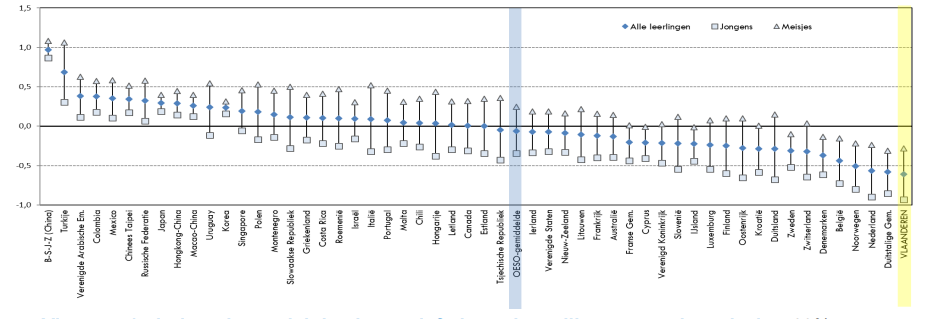
\includegraphics[width=\linewidth]{img/oeso-graphic-leesplezier.png}
	\end{center}
	\caption{Figuur van \textcite{DeMeyer2019}}
	\label{img:oeso-leesplezier}
\end{figure}

\medspace

% TODO dit toevoegen na einde van eerste zin: 

Intensief leesbegrip valt niet te omzeilen in onze huidige samenleving, maar dit leesbegrip verschilt enorm in het middelbaar onderwijs. Zo benadrukt de inspectie van \textcite{Vlaanderen2020} dat intensief lezen een essentiële vaardigheid is en een direct effect kan hebben op vakken buiten Nederlands, zoals bij het lezen van vraagstukken bij wiskundige vakken, of het begrijpen van vakjargon bij STEM-vakken. 

\medspace 

Een doelgroep die extra met intensief leesbegrip geconfronteerd wordt, zijn scholieren met dyslexie. Onderzoeken van \textcite{Bonte2020, VanDerMeer2022} schatten dat ongeveer 15\% van de Vlaamse scholieren in het middelbaar onderwijs een vorm van dyslexie heeft. Zo kunnen scholieren met dyslexie bij het intensief lezen geconfronteerd worden op een moeizame en stroeve automatisering bij het lezen en spellen. Hoewel scholieren met dyslexie ondersteuning kunnen krijgen, mag de impact van leesstoornissen niet onderschat worden. De gevolgen hiervan kunnen zich namelijk doorzetten na het middelbaar onderwijs. Leesvaardigheid blijft daarmee cruciaal voor succes op school en in het werkveld. Scholieren met dyslexie kunnen hebben met spelling, wat kan leiden tot onzekerheid en stress. Daarnaast zijn vooroordelen nog steeds een probleem en kunnen ze leiden tot stigmatisering. Echter toont onderzoek aan dat scholieren met dyslexie doorzettingsvermogen hebben en goede probleemoplossers zijn \autocite{Ghesquiere2018, Lissens2020, Bonte2020}. 

\medspace

Het leerplan voor STEM-vakken stimuleert het gebruik van wetenschappelijke artikelen, maar houdt niet altijd rekening met de bijhorende complexe leesgraad. De ingewikkelde woordenschat en syntax in wetenschappelijke artikelen kunnen een hindernis vormen voor de begrijpelijkheid van een tekst, waardoor scholieren met dyslexie de kerninhoud moeilijk kunnen doorgronden. Het handmatig vereenvoudigen van wetenschappelijke artikelen echter planning, tijd en energie van leerkrachten in de derde graad middelbaar onderwijs opslorpen. Het Vlaamse middelbaar onderwijs staat onder druk en docenten hebben moeite om met deze werkdruk boven water te blijven. 

\medspace

Nu is AI technologisch hoogstaand om tekstvereenvoudiging te automatiseren en om een baanbrekende oplossing aan te bieden aan het middelbaar onderwijs. Soortgelijke technologieën worden echter amper toegepast in het onderwijs. Er is terughoudendheid door enerzijds ouders van leerlingen \autocite{Martens2021a}, anderzijds door de weinige ontwikkelingen in schoolgerelateerde AI-software. Dit terwijl AI-ondersteuning in het onderwijs wel degelijk een positief effect heeft \autocite{Belpaeme2018, Kraft2020}. 

\medspace

Recente technologieën bieden reeds mogelijkheden tot tekstvereenvoudiging aan, maar zijn voorlopig enkel in commandline of met scripts ter beschikking. Voor het gebruik van taalmodellen of API's is uitgebreide informaticakennis nodig, waarover de meeste scholieren en leraren niet beschikken. Anderzijds zijn de huidige online tools te beperkt en eerder gericht op samenvatten; wat niet noodzakelijk bijdraagt tot een eenvoudigere tekst. Er is nood aan een intuïtieve en gebruikersvriendelijke toepassing die taalmodellen of API's kan integreren en aanpassen naargelang de specifieke behoeften van een student met dyslexie. Zo kan dit enerzijds ook de werkdruk bij leerkrachten verminderen, anderzijds om scholieren in de derde graad te ondersteunen bij het lezen van complexe wetenschappelijke artikelen. 

\section{\IfLanguageName{dutch}{Onderzoeksvraag}{Research question}}%
\label{sec:onderzoeksvraag}

Dit onderzoek beschrijft het gebruik van artificiële intelligentie in de vorm van tekstvereenvoudiging, als advies voor implementatie in het onderwijs. Specifiek om scholieren met dyslexie in de derde graad van het middelbaar onderwijs te ondersteunen bij het intensief lezen van wetenschappelijke artikelen. Hiervoor is de volgende onderzoeksvraag opgesteld: 

\begin{itemize}
	\item Hoe kan een wetenschappelijke artikel automatisch vereenvoudigd worden, gericht op de unieke noden van scholieren met dyslexie in de derde graad middelbaar onderwijs?
\end{itemize}

Om deze onderzoeksvraag te kunnen beantwoorden, moet een antwoord gezocht worden op de volgende deelvragen:

\begin{enumerate}
	% 1
	\item Welke specifieke noden hebben scholieren met dyslexie van de derde graad middelbaar onderwijs bij het begrijpen van complexere teksten? Aanvullend hierop: 
	\begin{itemize}
		\item Wat zijn de specifieke kenmerken van wetenschappelijke artikelen?
	\end{itemize} 
	% 2
	\item Welke aanpakken zijn er voor geautomatiseerde tekstvereenvoudiging?
	\begin{itemize}
		\item Hoe worden teksten handmatig vereenvoudigd voor scholieren met dyslexie?
		\item Welke toepassingen, tools en modellen zijn er beschikbaar om Nederlandse geautomatiseerde tekstvereenvoudiging met AI mogelijk te maken?
		\item Hoe kunnen geautomatiseerde tekstvereenvoudiging en gepersonaliseerde tekstvereenvoudiging gecombineerd worden?
	\end{itemize}
	%3 
	\item Met welke valkuilen bij taalverwerking met AI moeten ontwikkelaars rekening houden?
	%4 
	\item Welke functies ontbreken AI-toepassingen om geautomatiseerde tekstvereenvoudiging mogelijk te maken voor scholieren met dyslexie in de derde graad middelbaar onderwijs? 
	\begin{itemize}
		\item Welke manuele methoden voor tekstverereenvoudiging komen niet in deze tools voor?"
	\end{itemize}
	% 5
	\item Welke taalmodellen of LLM's zijn geschikt voor automatische tekstvereenvoudiging voor vereenvoudigde wetenschappelijke artikelen voor scholieren met dyslexie in de derde graad van het middelbaar onderwijs met dezelfde of gelijkaardige kwaliteiten als manuele tekstvereenvoudiging?
	% 6
	\item Hoe kan een intuïtieve lokale webtoepassing worden ontwikkeld die zowel scholieren met dyslexie als leerkrachten helpt bij het vereenvoudigen van wetenschappelijke artikelen met behoud van semantiek, jargon en zinsstructuren?
\end{enumerate}


\section{\IfLanguageName{dutch}{Onderzoeksdoelstelling}{Research objective}}%
\label{sec:onderzoeksdoelstelling}

Het onderzoek heeft als doel om de technologische en logopedische aspecten te identificeren die AI-ontwikkelaars in overweging moeten nemen bij het creëren van een op maat gemaakte AI-toepassing voor geautomatiseerde tekstvereenvoudiging, specifiek ontwikkeld voor scholieren in de derde graad. Het resultaat van dit onderzoek is een prototype voor een AI-toepassing voor tekstvereenvoudiging in de vorm van een webtool. De webtool heeft twee functies. Enerzijds kan de tool de inhoud van wetenschappelijke artikelen vereenvoudigen op basis van de specifieke behoeften van scholieren met dyslexie in de derde graad van het middelbaar onderwijs. Anderzijds biedt de tool een geautomatiseerde benadering voor lectoren om wetenschappelijke artikelen te vereenvoudigen op basis van geselecteerde parameters en deze vervolgens in een bruikbaar formaat (pdf of word) terug te geven. De invoer bij dit prototype is een wetenschappelijk artikel in tekst- of PDF-formaat.


\section{\IfLanguageName{dutch}{Opzet van deze bachelorproef}{Structure of this bachelor thesis}}%
\label{sec:opzet-bachelorproef}

De rest van deze bachelorproef is als volgt opgebouwd:

In Hoofdstuk~\ref{ch:stand-van-zaken} wordt een overzicht gegeven van de stand van zaken binnen het onderzoeksdomein, op basis van een literatuurstudie.

In Hoofdstuk~\ref{ch:methodologie} wordt de methodologie toegelicht en worden de gebruikte onderzoekstechnieken besproken om een antwoord te kunnen formuleren op de onderzoeksvragen. Eerst wordt er een requirementsanalyse uitgevoerd, gevolgd door de ontwikkeling van een prototype voor tekstvereenvoudiging.

\begin{enumerate}
	% 1
	\item Welke specifieke noden hebben scholieren met dyslexie van de derde graad middelbaar onderwijs bij het begrijpen van complexere teksten? Aanvullend hierop: 
	\begin{itemize}
		\item Wat zijn de specifieke kenmerken van wetenschappelijke artikelen?
	\end{itemize} 
	% 2
	\item Welke aanpakken zijn er voor geautomatiseerde tekstvereenvoudiging?
	\begin{itemize}
		\item Hoe worden teksten handmatig vereenvoudigd voor scholieren met dyslexie?
		\item Welke toepassingen, tools en modellen zijn er beschikbaar om Nederlandse geautomatiseerde tekstvereenvoudiging met AI mogelijk te maken?
		\item Hoe kunnen geautomatiseerde tekstvereenvoudiging en gepersonaliseerde tekstvereenvoudiging gecombineerd worden?
	\end{itemize}
	%3 
	\item Met welke valkuilen bij taalverwerking met AI moeten ontwikkelaars rekening houden?
	%4 
	\item Welke functies ontbreken AI-toepassingen om geautomatiseerde tekstvereenvoudiging mogelijk te maken voor scholieren met dyslexie in de derde graad middelbaar onderwijs? 
	\begin{itemize}
		\item Welke manuele methoden voor tekstverereenvoudiging komen niet in deze tools voor?"
	\end{itemize}
	% 5
	\item Welke taalmodellen of LLM's zijn geschikt voor automatische tekstvereenvoudiging voor vereenvoudigde wetenschappelijke artikelen voor scholieren met dyslexie in de derde graad van het middelbaar onderwijs met dezelfde of gelijkaardige kwaliteiten als manuele tekstvereenvoudiging?
	% 6
	\item Hoe kan een intuïtieve lokale webtoepassing worden ontwikkeld die zowel scholieren met dyslexie als leerkrachten helpt bij het vereenvoudigen van wetenschappelijke artikelen met behoud van semantiek, jargon en zinsstructuren?
\end{enumerate}

In Hoofdstuk~\ref{ch:discussie} worden de resultaten gegeven op dit onderzoek. In Hoofdstuk~\ref{ch:conclusie}, tenslotte, wordt de conclusie gegeven en een antwoord geformuleerd op de onderzoeksvragen. Daarbij wordt ook een aanzet gegeven voor toekomstig onderzoek binnen dit domein.
\chapter{\IfLanguageName{dutch}{Stand van zaken}{State of the art}}%
\label{ch:stand-van-zaken}

\section{Onderzoeken rond dyslexie}

Lezen is een essentieel onderdeel van ons dagelijks leven en speelt een belangrijke rol in onze communicatie en begrip. Dyslexie kan het functioneren in het dagelijks leven belemmeren. Het begrijpen van de noden en hindernissen voor een scholier met dyslexie is van belang om deze doelgroep te ondersteunen en hun kwaliteit van lezen te verbeteren. Deze sectie zal ingaan op de unieke noden en bespreken hoe mensen met dyslexie kunnen worden geholpen bij het lezen. De volgende onderzoeksvraag wordt in deze sectie beantwoordt: "Welke specifieke noden hebben scholieren met dyslexie van de derde graad middelbaar onderwijs bij het begrijpen van complexere teksten?"

\subsection{Centraal zicht op dyslexie}

Lezen is onnatuurlijk en volgens de geschiedenis van de mens een recent begrip. Pas 5000 jaar geleden werd de geschreven taal bedacht. Mensen worden niet met leesvaardigheid geboren, maar leren dit zelf aan en daarvoor moet het brein heringericht worden \autocite{Bonte2020, VanDerMeer2022}. Dyslexie betekent letterlijk 'beperkt lezen'. Het voorlezen kan radend, langzaam en letter-voor-letter verlopen. Goede woordenschat ontwikkeling of vaak voorlezen is een beschermende factor tegen dyslexie \textcite{Vellutino2004, Bonte2020}. Onderzoeken halen drie verschillende types van dyslexie aan, namelijk fonologische dyslexie, \textit{surface dyslexia} en \textit{deep dyslexia}. Dezelfde onderzoeken wijzen erop dat een overlap van kenmerken over de drie types heen mogelijk is \autocite{Rello2012, Vellutino2004}.

% De visuele cortex is een hersengebied dat instaat voor de aanschouwelijke waarneming en herkenning van objecten, zoals meubels of letters. Lezen traint dit gebied bij het herkennen van letters, maar dit is niet evident en vordering bij letterherkenning gebeurt pas na meerdere pogingen. 

\subsection{Centraal zicht op de doelgroep}

% De transparantie van de taal beïnvloedt volgens \textcite{APA2013} de prevalentie van dyslexie in een taalgebied. Spaans, Italiaans en Chinees zijn transparant en hebben een sterkere grafeem-foneem en foneem-grafeem koppeling. Zo is bijvoorbeeld slechts 1\% van de Chinese sprekers dyslectisch. Engels is een minder transparante taal waar klanken op verschillende manieren geschreven kunnen worden, bijvoorbeeld \textit{eight} en \textit{late}. De prevalentie van dyslexie ligt met 20\% dan ook hoger in Engelstalige landen. 

Onderzoek naar dyslexie richt zich vaak op kinderen in het kleuter- en lager onderwijs om de diagnose op jonge leeftijd vast te stellen en de meest geschikte ondersteuning te bieden. Een zwakke ondersteuning kan een sneeuwbaleffect veroorzaken, waarbij de uitdagingen van dyslexie worden meegedragen naar volgende levensfasen. Volgens onderzoek van \textcite{Lissens2020} wordt de leeftijdsgroep van jongvolwassenen en ouderen vaak over het hoofd gezien. Mensen met dyslexie ervaren moeilijkheden bij het lezen en schrijven en worden sociaal niet altijd begrepen. De onderzoeksresultaten bij een experiment van \textcite{VanVreckem2015} met zeventien kinderen wijst uit dat er een geïndividualiseerde analyse op maat nodig is bij begrijpend lezen. Onvoldoende beheerste leerstof en leesstrategieën per kind moet achterhaald worden om zo specifieke begeleiding te kunnen bieden. 

\subsection{Mogelijke drempels voor mensen met fonologische dyslexie.}

Mensen met fonologische dyslexie kunnen verschillende drempels ervaren, waaronder trage woordbenoeming, hardnekkig letter-voor-letter lezen, problemen met woordherkenning en -herinnering, letter- en klankvorming, homofonische of pseudo-homofonische woordenschat en begripsproblemen \autocite{Bonte2020, RiveroContreras2021, Zhang2021}. Het oefenen van pseudowoorden en het herkennen van woorden kan volgens \textcite{Filipak2020} helpen, evenals het gebruik van educatieve apps en software, e-books en luisterboeken, woordspelletjes en puzzels en tekst-naar-spraak technologie. Visuele ondersteuning met film en afbeeldingen kan het leesbegrip verbeteren en het gebruik van een grote woordenschat en redeneervermogen kan nuttig zijn. Schriftelijke expressie kan echter problematisch zijn.

\subsection{Bewezen effecten van tekstvereenvoudiging -en aanpassing bij scholieren met dyslexie}

Dyslexie kan zich op verschillende manieren uiten bij elke leeftijdsgroep. Een ondersteunende toepassing moet met een individuele analyse van de specifieke behoeften en uitdagingen van elke leerling in gedachten worden ontworpen \autocite{Gooding2022}. Instructies moeten op een begrijpelijke en geïndividualiseerde manier worden gepresenteerd om de leerlingen te helpen bij het begrijpen en toepassen van de informatie. Het is belangrijk om te erkennen dat dyslexie zich bij verschillende kinderen op verschillende manieren kan uiten. Een bijkomende stoornis heeft bijvoorbeeld geen impact op de spellingprestaties van een kind. Het is daarom belangrijk om een toepassing te ontwerpen met de diversiteit van dyslexie in het achterhoofd.

\begin{figure}[H]
	\begin{center}
		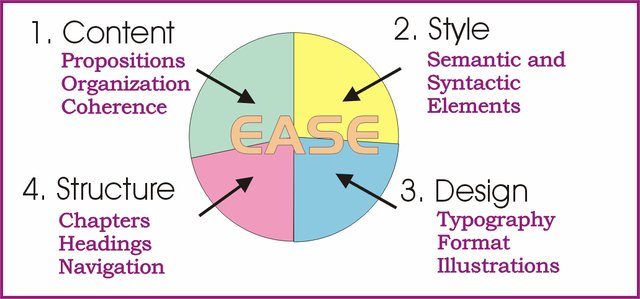
\includegraphics[width=9cm]{img/text-simplification-reading-ease.png}
	\end{center}
	\caption{Afbeelding van \textcite{Dubay2004}}
\end{figure}


\subsubsection{Lexicale wijzigingen}

Het onderzoek van \textcite{RiveroContreras2021} wijst uit dat teksten aanpassen, zoals lexicaal vereenvoudigen en samenvatten, een significant effect heeft op de leessnelheid en woordherkenning van een kind met visuele dysfunctie. Het experiment van \textcite{Rello2013a} wijst uit dat frequente woordenschat een significant verminderend effect heeft op de ontcijfertijd bij mensen met dyslexie significant vermindert wanneer de tekst een frequent woordgebruik toepast. De ontcijfertijd bij deelnemers met dyslexie waren significant lager bij het gebruik van frequente woordenschat dan bij minder frequente woordenschat.

\begin{figure}
	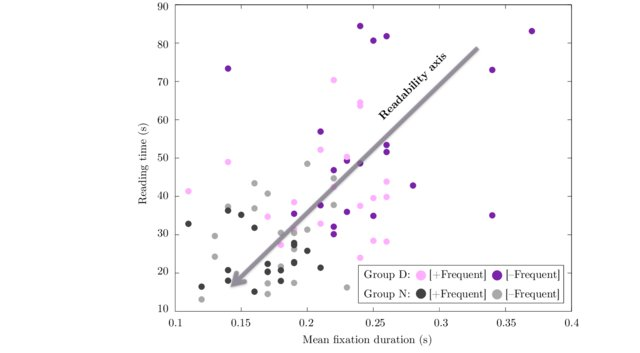
\includegraphics[width=\linewidth]{img/readability-mean-fixation-duration.png}
	\caption{Afbeelding van \textcite{Rello2013a}. Volgens de richting van de pijl wordt de ideale situatie benaderd, gekenmerkt door doelwaarden. Deze waarden worden bereikt door mensen zonder dyslexie onder optimale omstandigheden. Het gebruik van vaak voorkomende woorden vermindert de decodeertijd en verbetert de leesbaarheid voor mensen met dyslexie.}
\end{figure}

Bevraagden met dyslexie kunnen minder leesfouten maken bij een tekst met een verminderde lexicale complexiteit volgens \textcite{Gala2016}. De leessnelheid bij de kinderen lag hoger zonder een invloed op het begrip van de tekst. Het experiment benadrukt dat de bevraagden moeite hadden bij het lezen van woorden met meer dan zeven karakters. Daarnaast zorgden onregelmatige en infrequente lettergreepcombinaties voor moeilijkheden bij de bevraagde kinderen met dyslexie.

\subsubsection{Grammatische en syntactische wijzigingen}

Onderzoek rond de effecten op syntactische vereenvoudiging bij kinderen en scholieren met dyslexie zijn in schaarse hoeveelheid. Het aanpassen causale structuren bij kinderen en jongeren met een lage leesgraad had een significant effect op het leestempo en de foutenmarge van de bevraagden uit het experiment van \textcite{Linderholm2000}. Bij de revisies werden coherentieonderbrekingen werden hersteld door extra uitleg te voorzien, alsook door tekstgebeurtenissen in een temporele of tijdsafhankelijke volgorde te plaatsen. Zowel vaardige als minder vaardige lezers hadden baat bij de revisies. Verbale parafrasering heeft geen significant effect op lezers met dyslexie volgens \textcite{Rello2013c}. De bevraagden waren 13 tot en met 37 jaar oud met een gemiddelde leeftijd van 21 jaar. Het tekstformaat bleef ongewijzigd, maar lettertypes werden wel aangepast. 

\subsubsection{Wijzigingen op formaat en structuur}

Geassisteerd samenvatten bevoordeelt de leesbaarheid van een scholier met dyslexie volgens het experiment van \textcite{Nandhini2013}. De geassisteerde samenvatting is gebaseerd op onaangepaste zinnen afkomstig uit de oorspronkelijke tekst. Het ontwerp bij dit experiment haalt de belangrijkste zinnen onaangepast uit de oorspronkelijke tekst, herorganiseerd deze volgens de structuur van de oorspronkelijke tekst en presenteert deze aan de lezer. Al werd de logische structuur van de gepresenteerde zinnen in vraag gesteld, de leesbaarheid van de bevraagden was significant beter dan bij de oorspronkelijke tekst zonder een nadelig effect op de verstaanbaarheid van de bevraagden.

\subsubsection{Tekstweergave voor scholieren met dyslexie}

Uit experimenten op oogfixaties bleek dat scholieren met dyslexie gevoeliger zijn voor veranderingen in visuele parameters zoals lettertype, karakterafstand, tekst- en achtergrondkleur en grijswaarden. \textcite{Rello2015} beveelt een lichtgrijze achtergrond aan en een zwart lettertype op een gele achtergrond als beste kleurencombinatie. Zachtgele, -groene of lichtblauwe achtergrondkleuren verbeteren de leeservaring van scholieren met dyslexie in lager en middelbaar onderwijs \autocite{Bezem2016, Rello2017}. Het is belangrijk dat de eindgebruiker zelf een kleurschema kan kiezen. Minimalistische ontwerpen met pictogrammen en statische inhoud kunnen mensen met dyslexie helpen zich te concentreren op belangrijke informatie volgens \textcite{Anthony2020}. Afbeeldingen en schema's hebben ook een positief effect op de leesbaarheid van tekst \autocite{Rello2012b}. Er zijn geen duidelijke aanbevelingen voor grijswaarden en de keuze kan afhankelijk zijn van individuele voorkeuren. Bij het leren schrijven worden letters vaak in spiegelbeeld geschreven, wat nadelig kan zijn voor de leestijd van scholieren met dyslexie \autocite{Bonte2020, Romanovska2021}. Het lettertype en de grootte kunnen de leessnelheid en decodeertijd van scholieren met dyslexie beïnvloeden. Onderzoek toont aan dat een lettergrootte groter dan 14pt en een sans-serif, \textit{monospaced} of \textit{roman} lettertype de leessnelheid vergroten. Het gebruik van lettertypes zoals OpenDys heeft geen effect op lezers met of zonder dyslexie, terwijl cursieve lettertypes worden afgeraden \autocite{Rello2013b, Rello2015}.

\begin{figure}[H]
	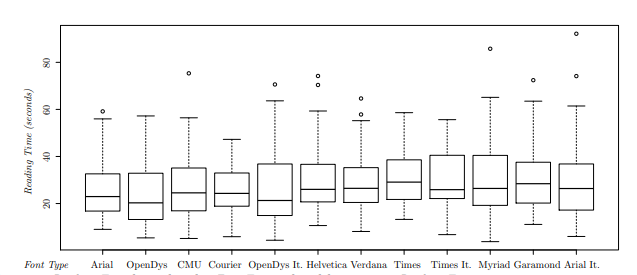
\includegraphics{img/fonts-readability.png}
	\caption{Afbeelding uit \textcite{Rello2013b}. Verticaal wordt de gemiddelde mening van de bevraagden weergegeven. Horizontaal worden de lettertypes gerangschikt op gemiddelde leestijd van alle bevraagden. Dit onderzoek wijst uit dat Arial, CMU, Helvetica en Times de populaire keuzes zijn. Arial en CMU behoren hierbij tot de drie best scorende lettertypes rond gemiddeld leestempo.}
\end{figure}

\subsection{Conclusie}

Op basis van de literatuurstudie kan besloten worden dat het aanpassen van teksten een significant effect heeft op de leessnelheid en woordherkenning van jongeren met dyslexie. Het vereenvoudigen van de lexicon en het toepassen van frequente woorden zorgt voor een verminderde decodeertijd en verbetert de leesbaarheid van teksten. Bevraagden met dyslexie hebben minder moeite met het lezen van teksten met verminderde lexicale complexiteit en geassisteerd samenvatten van teksten verbetert de leesbaarheid. Ook het aanpassen van de tekstweergave, zoals het gebruik van zachtgele, -groene of lichtblauwe achtergrondkleuren, kan de leeservaring van scholieren met dyslexie verbeteren. Het onderzoek rond de effecten op syntactische vereenvoudiging bij kinderen en jongeren met dyslexie is echter beperkt.

\section{Wetenschappelijke artikelen}

Wetenschappelijke artikelen volgen een uniform IMRAD-formaat en worden gebruikt als leermiddel voor jongeren in het middelbaar en hoger onderwijs. Het lezen van deze artikelen brengt uitdagingen met zich mee vanwege de verschillen in syntax en woordenschat. Docenten kunnen dit aanpakken in de derde graad van het middelbaar onderwijs door te benadrukken wat de specifieke kenmerken van wetenschappelijke artikelen zijn. In deze sectie wordt de volgende onderzoeksvraag beantwoordt: "Wat zijn de specifieke kenmerken van wetenschappelijke artikelen?"

\subsection{Wetenschappelijke geletterdheid in Vlaanderen}

De \textit{Programme for International Student Assessment} of PISA-test\footnote{https://www.pisa.ugent.be/resultaten/pisa-2022} van OESO is een driejaarlijkse test bij vijftienjarigen. Deze test bestudeert de wiskundige en wetenschappelijke geletterdheid\footnote{“Het beheersen van vaardigheden om als kritische burger om te gaan met wetenschappelijke onderwerpen en ideeën.” volgens \textcite{DeMeyer2019}} van 15-jarigen in geïndustrialiseerde landen, wat op ongeveer 79 landen komt. 4822 Vlaamse scholieren van vijftien jaar namen deel aan deze test. Dit onderzoek baseert op de cijfers van 2018, aangezien de testen van 2022 pas eind 2023 worden gepresenteerd. Deze testen houden echter geen rekening met leer- en leesstoornissen, waaronder dyslexie en dyscalculie. Het is echter nodig om deze cijfers mee te geven, om een idee te geven waar de doelgroep staat voor de start van de derde graad middelbaar onderwijs. 

De PISA-test\footnote{https://www.pisa.ugent.be/resultaten/pisa-2022} is een driejaarlijkse test bij vijftienjarigen in ongeveer 79 geïndustrialiseerde landen die de wiskundige en wetenschappelijke geletterdheid meet. 4822 Vlaamse scholieren van vijftien jaar namen deel aan deze test, gebaseerd op de cijfers van 2018. Leer- en leesstoornissen worden niet meegenomen in deze testen, maar bieden een perspectief op de leesvaardigheid en wetenschappelijke geletterdheid van scholieren van vijftien jaar.

\begin{figure}[H]
	\begin{center}
		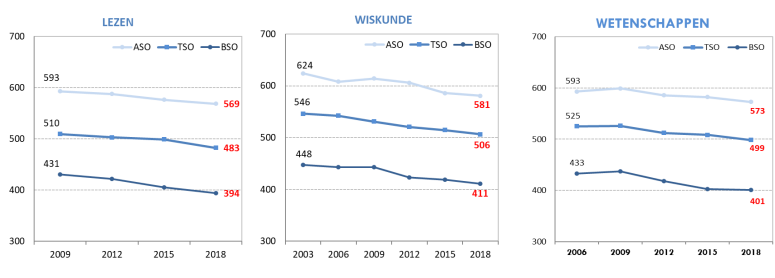
\includegraphics[width=\linewidth]{img/oeso-graphic-pisa-trend-samenvatting.png}
	\end{center}
	\caption{Figuur van \textcite{DeMeyer2019}. Op alle PISA-domeinen scoren de Vlaamse vijftienjarigen in ASO, BSO en TSO significant slechter dan de eerste metingen. \textcite{DeMeyer2019} noemen dit een achteruitgang in alle onderwijsvormen.}
\end{figure}

\begin{figure}[H]
	\begin{center}
		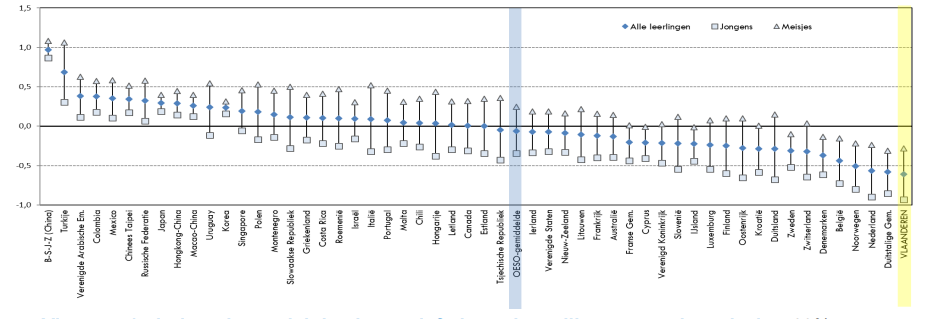
\includegraphics[width=\linewidth]{img/oeso-graphic-leesplezier.png}
	\end{center}
	\caption{Figuur van \textcite{DeMeyer2019}. Het leesplezier van Vlaamse 15-jarigen. Zij uitten zich uiterst negatief op stellingen over leesplezier. Volgens de enquète vond de helft van de scholieren begrijpend lezen enkel tijdsverlies en slechts 17\% gaf aan dat lezen één van hun favoriete hobby's is. Er is wel een significant verschil tussen de mening van jongens en meisjes, waar jongens negatiever antwoorden op lezen.}
\end{figure}

\begin{figure}[H]
	\begin{center}
		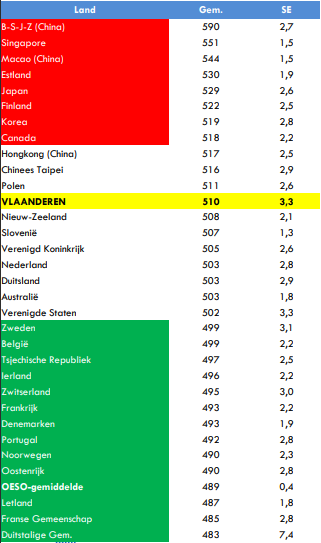
\includegraphics[width=5cm]{img/oeso-graphic-wetenschappelijke-geletterdheid-2.png}
	\end{center}
	\caption{Figuur van \textcite{DeMeyer2019}. De wetenschappelijke geletterdheid bij vijftienjarigen op internationaal niveau. Vlaanderen scoort significant slechter dan acht deelnemende landen.}
\end{figure}


\subsection{Trends rond wetenschappelijke artikelen}
% inleiding over het formaat van teksten

De leesgraad van wetenschappelijke teksten volgt al sinds de tweede helft van de twintigste eeuw een stijgende trend \autocite{Hayes1992}. Meerdere onderzoeken in de voorbije tien jaar besluiten dat de complexe woordenschat en zinsbouw deze wetenschappelijke artikelen ontoegankelijk maakt voor doelgroepen naast onderzoekers \autocite{Ball2017, PlavenSigray2017, Jones2019}. 

% \textcite{Ball2017}

\textcite{PlavenSigray2017} onderzoekt de verschillende trends waarom wetenschappelijke artikelen alsmaar moeilijker te lezen worden. De relatie tussen de leesbaarheid van een abstract werd vergeleken met het jaar waarin het wetenschappelijk artikel werd gepubliceerd. De \textit{Flesch-Reading-Ease} of FRE score werd gebruikt om de leesgraad van een wetenschappelijk artikel te beoordelen. Om te bevestigen dat de relatie tussen de complexiteit van een abstract overeenstemt met die van de volledige tekstinhoud, werden er vergelijkingen gemaakt met zes verschillende wetenschappelijke journalen. De overeenkomst tussen de leesgraad van het abstract en de overige tekstinhoud in een wetenschappelijk artikel werd eerder bevestigd door \textcite{Dronberger1975}. Dat onderzoek benadrukte dat een abstract complexer werd geschreven, vergeleken met de rest van een wetenschappelijk artikel.

\begin{figure}[H]
	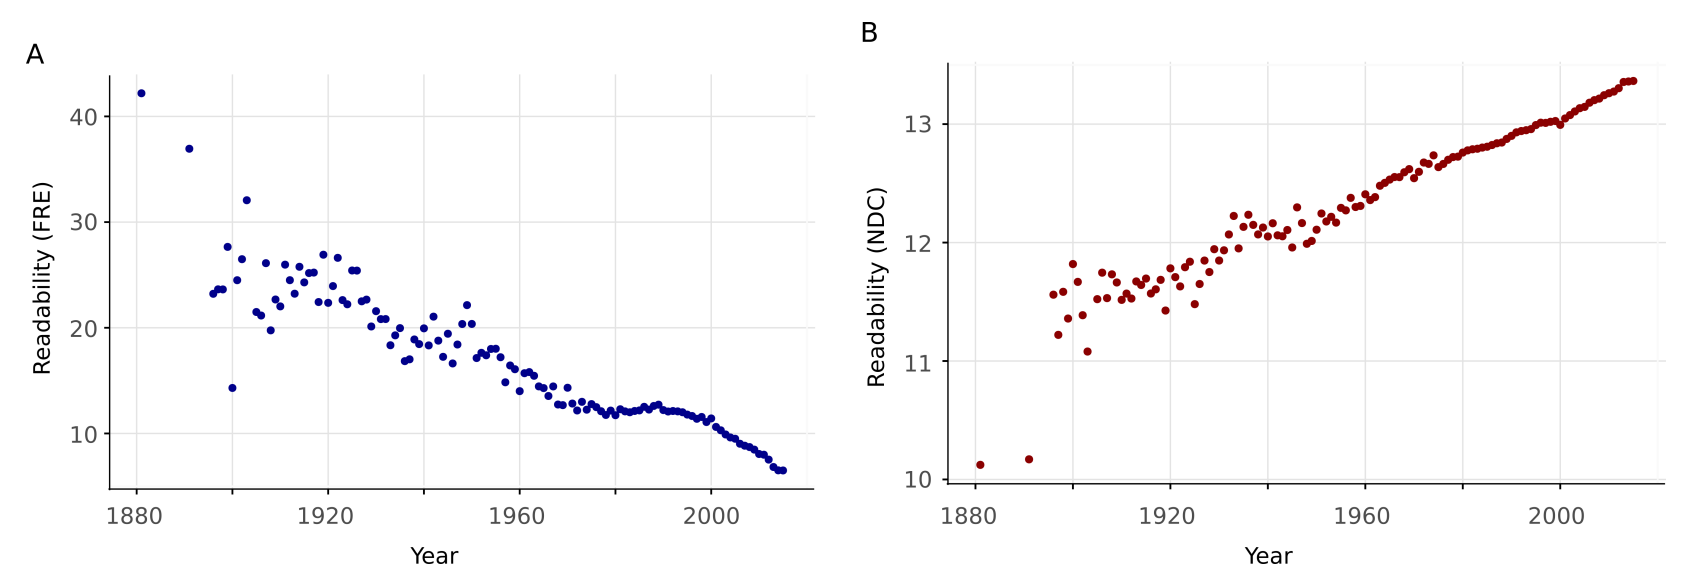
\includegraphics[width=\linewidth]{img/fre-ndc.png}
	\caption{Afbeelding uit \textcite{PlavenSigray2017}. Links wordt de evolutie per FRE-score getoond. Hoe hoger de score, hoe hoger de gemiddelde complexiteit van een tekst. Rechts wordt de evolutie volgens de NDC-score getoond. Hoe hoger de score, hoe lager de gemiddelde complexiteit van een tekst. Het onderzoek schat dat nu een kwart van alle wetenschappelijke artikelen gebruik maken van Engels op het niveau van een masterstudent, ofwel een FRE onder nul.}
\end{figure}

\begin{figure}[H]
	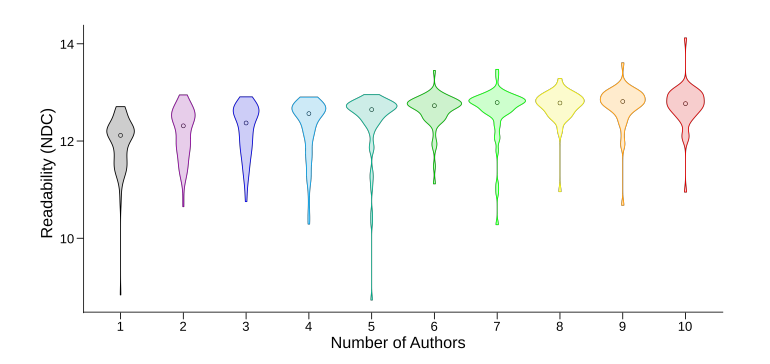
\includegraphics[width=\linewidth]{img/ndc-number-of-authors.png}
	\caption{Afbeelding uit \textcite{PlavenSigray2017}. Horizontaal worden het aantal auteurs per wetenschappelijk artikel aangeduidt. Verticaal wordt de gemiddelde NDC-score weergegeven. HOe hoger de NDC-score, hoe hoger de vereiste leesgraad om de tekst te kunnen lezen.}
\end{figure}

De hoge leesgraad van wetenschappelijke artikelen beperkt volgens \textcite{PlavenSigray2017} twee aspecten: de toegankelijkheid en de herproduceerbaarheid.

\subsubsection{Toegankelijkheid}

Bronnen worden minder toegankelijk tot het algemene publiek. Wetenschappelijke artikels worden enkel toegankelijk tot mensen die wetenschappelijk geletterd zijn of een leesgraad daarboven hebben. \textcite{Ennals2010} zegt dat wetenschap ons de nauwkeurige kennis moet geven, omdat mensen zich zorgen maken dat moderne samenlevingen minder streng worden met feitelijke waarheden en deze vervangen door \textit{post-facts} die waar lijken te klinken. Wetenschappelijke inhoud moet volgens hem zo toegankelijk mogelijk worden gemaakt, zodat een zo breed mogelijk publiek de kern begrijpt.

\subsubsection{Reproduceerbaarheid}

Onbegrijpelijke en ontoegankelijke zinsstructuren hinderen ook vakexperten. Het herschrijven van abstracten vergroot de begrijpbaarheid bij academici volgens \textcite{Hartley1999, Snow2010}. De wetenschap bouwt voort op betrouwbare ontdekkingen en het reproduceren van experimenten is een belangrijke manier voor wetenschappers om vertrouwen te krijgen in hun besluiten. De inhoud van het wetenschappelijke artikel moet gecontroleerd kunnen worden. Voor de reproduceerbaarheid van onderzoeken is het volgens \textcite{McNutt2014} belangrijk dat de methodologie en resultaten begrijpelijk zijn. Een lage leesgraad en duidelijke zinsbouw beperkt het aantal misopvattingen en verwarringen bij onderzoekers. Experimenten uit \textcite{Hubbard2017} wijzen erop dat de bevraagde onderzoekers zowel de methodologie als de resultaten de twee componenten vonden die een hoge leesgraad vergden. 

% https://psychology.ucsd.edu/undergraduate-program/undergraduate-resources/academic-writing-resources/writing-research-papers/research-paper-structure.html#:~:text=A%20complete%20research%20paper%20in,%2C%20Discussion%2C%20and%20References%20sections.&text=Many%20will%20also%20contain%20Figures,have%20an%20Appendix%20or%20Appendices.

\subsection{Woordenschat en vakjargon}

Complexe processen, methoden en ideeën worden in wetenschappelijke artikelen verwoord met gebruik van grammatische embeddings, doordachte en abstracte woordenschat en naamwoordstijlen. De kenmerken van academische taal variëren afhankelijk van de discipline, het onderwerp en de vorm, maar er zijn gemeenschappelijke kenmerken die wetenschappelijke taal onderscheiden van taal van een lagere leesgraad. \autocite{Ennals2010, Snow2010}

Wetenschappelijke artikelen dienen volgens \textcite{PlavenSigray2017} in eerste instantie als uitwisseling van kennis tussen vakexperten. Daarnaast moet er rekening worden gehouden met de lengte wat een nadelig effect heeft op de beschikbare uitleg voor deze terminologie.

\textcite{Snow2010} beklemtoont dat deze zaken in het onderwijs moeten betrokken worden. STEM-vakken of vakken waar deze wetenschappelijke artikelen aan bod komen, moeten stil staan bij voldoende uitleg over de toegepaste grammatica en woordenschat voorzien tijdens de lessen.

\begin{figure}[H]
	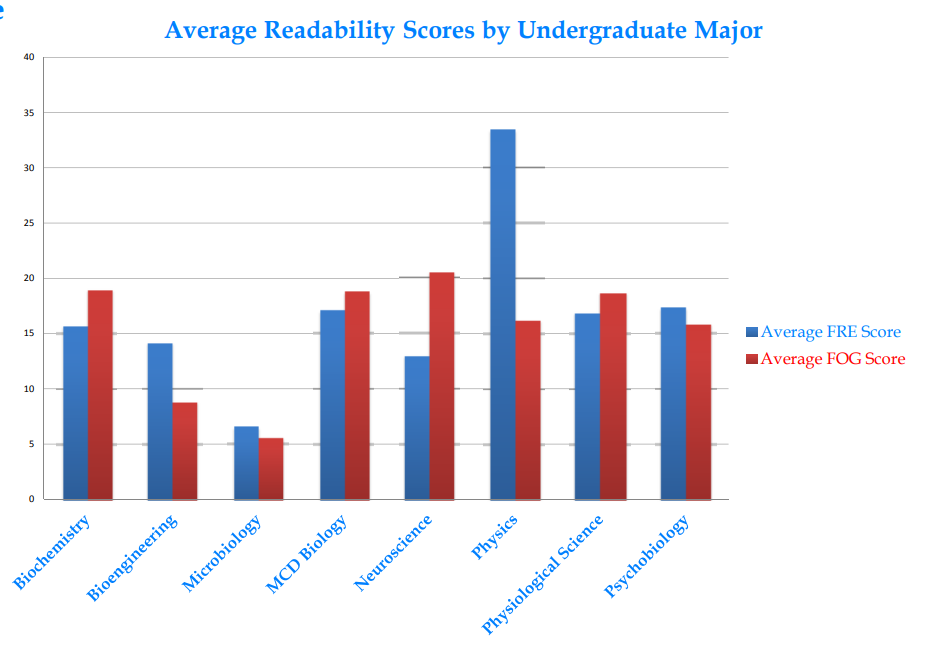
\includegraphics[width=5cm]{img/fre-fog-per-sector.png}
	\caption{Afbeelding van \textcite{Murdos2014} Volgens deze grafiek scoren de wetenschappelijke artikels rond fysica gemiddeld het best op de FRE-score. Al scoren de wetenschappelijke artikels rond microbiologie gemiddeld het zwakst op de FRE-score, ze scoren gemiddeld beter op de FOG-score.}
\end{figure}

\subsection{Aanpak voor het lezen van wetenschappelijke artikelen}

Als reactie op een satirisch artikel van \textcite{Ruben2016}, bracht \textcite{Pain2016} het onderwerp bij wetenschappers aan het licht om zo verschillende tactieken te verzamelen om wetenschappelijke artikelen te begrijpen. Sommige wetenschappers zoeken direct onbekende woorden op of raadplegen extra informatiebronnen, terwijl andere wetenschappers hoofdstukken overslaan. Het is belangrijk om een balans te vinden tussen het begrijpen van de inhoud en het efficiënt gebruiken van de tijd. Sommige wetenschappers geven toe dat ze het soms opgeven als het te moeilijk wordt of als de literatuur net niet relevant is voor hun onderzoek. {Pain2016} bouwt verder op deze adviezen en bouwt een stappenplan op hoe (startende) lezers wetenschappelijke artikelen kunnen aanpakken.

\begin{enumerate}
	\item Lees de samenvatting en conclusie om een idee te krijgen van het doel en de uitkomst van het onderzoek.
	\item De figuren en tabellen in het artikel zijn cruciaal omdat deze een snelle en duidelijke weergave geven van de belangrijkste bevindingen.
	\item Focus op de nodige informatie en ga vervolgens terug om de technische details te begrijpen.
	\item Let op de beperkingen en interpretatie van de resultaten. Controleer of de onderzoeksvraag en -methode adequaat zijn.
	\item Controleer of de referenties relevant zijn en zoek naar andere artikelen over hetzelfde onderwerp.
	\item Overweeg welke stukken prikkelend, nieuw en relevant zijn voor eigen onderzoeksvragen en hypotheses.
	\item Maak aantekeningen en schrijf tijdens het lezen, zodat de lezer actief betrokken is bij het lezen van het artikel.
\end{enumerate}

Wetenschappelijke artikelen vereisen een selectieve leesstijl volgens de bevraagde onderzoekers in \textcite{Hubbard2017}. Bepaalde delen van een artikel worden geprioriteerd, zoals de abstract. De abstract en de discussie bepaalt of het artikel de moeite waard is voor de onderzoeker om te lezen. Sommige bevraagden adviseren om de methodologie te negeren en direct over te gaan naar de discussie of resultaten, terwijl andere onderzoekers aanbevelen om eerst de hypothesen van een artikel te achterhalen. Een artikel wordt nadrukkelijk meermaals gelezen, waarbij de lezer steeds in meer detail leest. Kritisch lezen is belangrijk, waarbij de conclusies worden beoordeeld en de data voor zichzelf spreekt. Er is geen standaardaanpak volgens \textcite{Hubbard2017}, maar de bevraagde onderzoekers bevelen tactieken aan zoals selectief, kritisch en met een specifiek doel voor ogen lezen.

\subsection{Conclusie}

Het lezen van wetenschappelijke artikelen kan overweldigend zijn, vooral bij onbekende vakgebieden, lange artikelen en technisch vakjargon. Nieuwe versies van een wetenschappelijk artikel moeten meer doelgroepen toelaten om over voldoende achtergrondinformatie te beschikken. De gebruikte syntax, woordenschat en compact formaat sluiten aan bij de mogelijke struikelblokken voor ee scholier met dyslexie in de derde graad van het middelbaar onderwijs. 

\section{Tekstvereenvoudiging}

Vereenvoudigde teksten worden geschreven om leerlingen te ondersteunen bij het begrijpen van specifieke taalkenmerken, het beperken van de hoeveelheid nieuwe woordenschat en het beheersen van de complexiteit van de tekst. Deskundigen zijn van mening dat vereenvoudigde teksten nuttig zijn voor startende en gevorderde lezers \autocite{Louwerse2007}. Samenvattingen van teksten bieden een oplossing om een snel zicht te krijgen over (lange) documenten, of om de kerninhoud van een tekst die al gelezen is opnieuw te prikkelen \autocite{McCombes2022}. Vereenvoudigen kan handmatig door de docent gebeuren, maar recente technologische ontwikkelingen laten de automatisatie van dit proces toe met een gelijkwaardig eindresultaat. Deze sectie beantwoordt de volgende onderzoeksvraag: "Welke aanpakken zijn er voor geautomatiseerde tekstvereenvoudiging?". Aansluitend hierop wordt de volgende subvraag beantwoordt: "Hoe worden teksten handmatig vereenvoudigd voor scholieren met dyslexie?"

\subsection{Manuele tekstvereenvoudiging}

Wetenschappelijke artikelen moeten informatie begrijpelijk weergeven voor een breed publiek, waaronder de scholieren die deze artikelen voorgeschoteld krijgen. Teksten vereenvoudigen heeft volgens \textcite{Crossley2012} drie algemene doelen, namelijk het illustreren van een specifiek taalkenmerk, ongekende woordenschat voor een doelgroep aan te passen en de hoeveelheid gegeven informatie onder controle te houden. \textcite{Crossley2012} wijst op twee soorten van handmatige tekstvereenvoudiging. Intuïtieve tekstvereenvoudiging is een methode waar de auteur die de transformatie uitvoert, wordt beïnvloed door persoonlijke vermoedens over wat een tekst beter leesbaar maakt. Structurele vereenvoudiging daarentegen vervangt vermoedens door het gebruik van woordenlijsten en leesbaarheidsformules zoals Flesch Reading Ease (FRE), Gunning Fog (FOG), SMOG-Cro (SMOG) en de Coleman-Liau Index (CLI).

\subsubsection{Lengte en formaat}

Een samenvatting verkort de lengte van een tekst. Kernzinnen en trefwoorden worden eerst handmatig in een tekst gemarkeerd en vervolgens op een nieuw blad geschreven. De kernzinnen worden achterhaald door enerzijds woord- en zoektermfrequentie en anderzijds door het stellen van algemene vragen over het artikel. Trefwoorden achterhalen gebeurt gelijkaardig en deze zijn regelmatig af te leiden uit de inhoudstafel en titels. Voor deze twee methoden moet de persoon die een samenvatting maakt al vooraf de tekst meermaals gelezen hebben. Een alternatief op markeren is het parafraseren van de tekst. De geparafraseerde tekst is semantisch identiek, maar het neemt een andere syntax, structuur en woordenschat aan \autocite{Rijkhoff2022}.

Volgens \textcite{Hahn2000} kan een samenvatting informatief, indicatief of kritisch zijn. Informatieve samenvattingen vervangen de oorspronkelijke tekst. Hoofd- en bijzaken zijn betrokken in de samengevatte tekst. Indicatieve samenvattingen behouden enkel een tekst met links die een lezer doorverwijzen naar andere bronnen. Kritische samenvattingen of \textit{reviews} bestaan uit de kerninhoud van de oorspronkelijke tekst en een opiniestuk over die specifieke kerninhoud. Tekstvereenvoudiging omvat conceptuele of semantische vereenvoudiging door complexe concepten op te splitsen en duidelijke taal te gebruiken, pragmatische vereenvoudiging en het aanpassen van de alinea-indeling door middel van opsommingen. Het doel is om de tekst begrijpelijk te maken zonder betekenis of nauwkeurigheid te verliezen. Een opsomming of oplijsting benadrukt belangrijke punten en maakt een duidelijke structuur van een mogelijks complexe tekst \autocite{Siddharthan2014, Hale2022}. Pragmatische vereenvoudiging zet metaforen, \textit{short language} of \textit{slang} en idiomen om naar een letterlijke en duidelijke tekst \autocite{JavoureyDrevet2022}.

Verder haalt \textcite{Hahn2000} ook het onderscheid tussen een generieke en een gebruikersgerichte samenvatting. Een generieke samenvatting staat niet stil bij speciale noden of interesses van de eindgebruiker in tegenstelling tot een gebruikersgerichte samenvatting waarbij er wel met sleutelwoorden of thema's in een tekst wordt rekening gehouden. \textcite{Hahn2000} haalt aan dat technologieën zoals \textit{full-text-search} en gepersonaliseerde informatiefiltering het belang van gebruikersgerichte samenvatting naar voor duwen. De opbouw van een gebruikersgerichte samenvatting omvat drie fasen volgens \textcite{Hahn2000}. Allereerst wordt de brontekst geanalyseerd. Daarna worden de kernpunten in een tekst aangeduid. Deze kernpunten kunnen verschillen per auteur. Ten slotte worden de punten samengevoegd tot één uitvoertekst.

Volgens \textcite{Hollenkamp2020, McCombes2022} moet een samengevat wetenschappelijk artikel drie vragen kunnen beantwoorden: 

\begin{itemize}
	\item Waarom werd het onderzoek verricht? Welke achtergrondinformatie en context nam de onderzoeker in acht. Daarnaast moeten de geformuleerde hypotheses aan bod komen.
	\item Wat werd er geëxperimenteerd? Alle gebruikte methoden en resultaten moeten in een samenvatting terug te vinden zijn en enkel de noodzakelijke kwalitatieve waarden mogen aan bod komen.
	\item Welke conclusies trekken de onderzoeker(s) uit het onderzoek? De implicaties en beperkingen tijdens het onderzoek, alsook de aanradingen moeten in de samenvattingen aan bod komen.
\end{itemize}

Vervolgens kan tekst naar een ander formaat worden omgezet, zoals \textit{post-itnotes}, \textit{postcards} of emails, om het begrijpelijker te maken. Dit wordt vooral ingezet in het lager onderwijs. De schrijf- en vertelstijl moet consistent blijven in het nieuwe formaat. Ten slotte moeten verwijswoorden worden aangepast om de tekst toegankelijker te maken voor meertalige lezers. Bijvoorbeeld door eenvoudige verwijswoorden zoals 'zij' of namen te gebruiken \autocite{Rijkhoff2022}. 

\subsubsection{Pedagogische en onderwijsgerelateerde kritieken}

Het onderzoek van \textcite{Crossley2012} wijst het bevorderend effect van de unieke aanpakken per docent uit. Iedere docent heeft een eigen intuïtie of afweging waarop teksten kunnen worden vereenvoudigd. Er is geen uniform formaat waarin een tekst kan worden vereenvoudigd. 

\subsection{Natural Language Processing}

Tekstvereenvoudiging is het proces waarin het technisch leesniveau en/of woordgebruik van een geschreven tekst wordt verminderd. Het resultaat van deze fase is een tekst die korter en aangenamer is, zonder het verlies van de kerninhoud. Binnen machinaal leren (ML) is tekstvereenvoudiging een zijtak van natuurlijke taalverwerking. \autocite{Siddharthan2006} Volgens \autocite{Siddharthan2014} bestaat een complete en geautomatiseerde tekstvereenvoudiging uit vier verschillende vereenvoudigingen. \textit{Natural Language Processing} (NLP) of natuurlijke taalverwerking is een brede term die zich richt op het verwerken en analyseren van menselijke taal door computers \autocite{Eisenstein2019}. NLP omvat verschillende technieken, zoals tekstanalyse, taalherkenning en -generatie, spraakherkenning en -synthese, en semantische analyse. Computers zijn in staat om op een menselijke manier te communiceren en begrijpen wat er wordt gezegd. De volgende begrippen worden aangehaald in \textcite{Sohom2019, Eisenstein2019} en zijn fundamenteel voor de concepten die volgen.

\subsubsection{Tokenisation}

Tokenisatie} splitst de stam of basisvorm van woorden in een tekst. Gebruikelijk zetten ontwikkelaars deze stap in om een woordenschat voor een taalmodel op te bouwen. Bij tokenisatie wordt er geen rekening gehouden met de betekenis achter ieder woord. Tokeniseren kan volgens \textcite{Menzli2023} op vier manieren:

\begin{itemize}
	\item Word-level tokenisation of WTL splitst de tekst op per woord.
	\item Character-level tokenisation of CLT splitst de tekst per karakter. 'Slimmer' wordt s-l-i-m-m-e-r. Deze vorm achterhaalt de semantiek van een tekst beter en laat de het. Nadelig hebben de karakters op zich weinig betekenis, alsook maakt deze vorm de inputlengte groter. \autocite{Ribeiro2018}
	\item Subword-level tokenisation splitst de tekst op in stukken op basis van de woordfrequentie. Veelvoorkomende woorden worden hele woorden getokeniseerd, terwijl zeldzamere woorden opgesplitst worden in kleinere stukken die kunnen worden gebruikt. De rest van de woorden in de relevante dataset te creëren. Dit biedt een voordeel ten opzichte van word-level tokenisation omdat het een balans biedt tussen WLT en CLT \autocite{Iredale2022}.
	\item Sentence tokenization splitst de tekst op per zin. \textcite{Fardeen2021} haalt aan dat de tokenizer ineffectief is tegen afkortingen, maar dit is afhankelijk volgens de gebruikte dataset. 
\end{itemize}

\subsubsection{Lemmatiseren en parsen}

Lemmatiseren in NLP bouwt verder op \textit{stemming}, maar de betekenis van ieder woord wordt in acht genomen. Voor het lemmatiseren bestaan er Nederlandstalige modellen, waaronder JohnSnow\footnote{https://nlp.johnsnowlabs.com/2020/05/03/lemma\_nl.html}. Bij \textbf{omgekeerd lemmatiseren} wordt er een afgeleide achterhaald vanuit de stam. Bijvoorbeeld voor het werkwoord 'zijn' zou dit 'is', 'was' of 'ben' zijn. Voor zelfstandige naamwoorden, zoals 'hond', is dit dan enkelvoud of meervoud \autocite{Eisenstein2019}.

Bij een \textbf{parsing}-fase wordt er een label aan ieder woord of zinsdeel toegekend. Voorbeelden van labels zijn zelfstandig naamwoord, bijwoord, werkwoord, bijzin of stopwoord. Het herkennen van zinsdelen wordt \textit{chunking} genoemd. Parsing heeft een dubbelzinnigheidsprobleem, want een 'plant' staat niet gelijk aan de vervoeging van werkwoord 'planten' \autocite{Eisenstein2019}.

% Sentimentanalyse is het achterhalen van de mening of gevoelens uit een tekst. de stemming of mening van een tekst te achterhalen op basis van het onderwerp. is een tak van Natural Language Understanding of NLU die de stemming, mening of gevoelens van de schrijver of spreker probeert te achterhalen ten opzichte van het onderwerp. % Dit kan lastig zijn omdat niet elke tekst een duidelijk positief of negatief sentiment heeft. 

\subsubsection{Sequence labeling en part-of-speech tagging}

Een machine moet de betekenis achter ieder token kunnen vatten. Hier komt \textit{sequence labeling} aan de pas volgens \textcite{Eisenstein2019}. Elk woord in een tekst wordt gekoppeld aan een \textit{Part-of-Speech} (PoS) of \textit{Named-Entity-Recognition} (NER) label. Deze NLP-fase achterhaalt de structuur van een tekst. PoS-tagging richt zich op grammaticale categorieën van woorden, terwijl NER-labeling instaat voor het herkennen van specifieke entiteiten in een tekst. Bij PoS-tagging worden de woorden in een zin geanalyseerd. Elk woord wordt gekoppeld aan een grammaticale categorie, zoals een zelfstandig naamwoord, werkwoord, bijvoeglijk naamwoord of bijwoord. \textit{PoS-tagging} helpt bij het achterhalen van de syntactische structuur van een zin. Deze taak komt van pas bij parsing en machinevertaling. \textit{PoS-tagging} wordt aanschouwelijk gemaakt op \ref{fig:pos}. Namen van personen, organisaties en locaties worden herkend en geclassificeerd met NER-labeling. Met NER-labeling wordt volgens \textcite{Jurafsky2014} specifieke informatie uit tekst gehaald, zoals het identificeren van de namen van personen, plaatsen of bedrijven die in nieuwsartikelen worden genoemd, of het extraheren van belangrijke data of getallen uit financiële rapporten. Dit wordt aanschouwelijk gemaakt \ref{fig:ner}. \textcite{Li2018} benoemt vier vormen voor NER-labeling:

\begin{itemize}
		\item \textit{Dictionary-based NER labeling} gebruikt vooraf gedefinieerde woordenboeken die de namen van de entiteiten bevatten.
		\item \textit{Rule-based NER labeling} gebruikt vooraf gedefinieerde regels die gebaseerd zijn op syntactische of semantische patronen om de entiteiten te identificeren.
		\item \textit{Machine learning-based NER labeling} gebruikt statistische modellen zoals Hidden Markov Model (HMM) of Conditional Random Field (CRF) om te leren van gelabelde trainingsgegevens hoe ze entiteiten kunnen herkennen. Het gebruikt kenmerken zoals het woord zelf, omliggende PoS-labels en het hoofdlettergebruik om te beslissen welk label aan elk woord moet worden toegekend.
		\item Deep learning-based NER labeling gebruikt neurale netwerken zoals recurrent neural network (RNN) of convolutional neural network (CNN) om te leren van ongelabelde of gedeeltelijk gelabelde trainingsgegevens hoe ze entiteiten kunnen herkennen. Het gebruikt woordvectoren en niet-lineaire representaties om complexe relaties tussen woorden te modelleren.
\end{itemize}

\textcite{Poel2008} onderzocht \textit{PoS-tagging} met een neuraal netwerk voor Nederlandstalige teksten. Het model behaalde een nauwkeurigheid van 97,88\% voor bekende woorden en 41,67\% voor onbekende woorden. Het model gebruikte de Corpus Gesproken Nederlands (CGN) als trainingsdata.

\begin{figure}[H]
	\begin{center}
		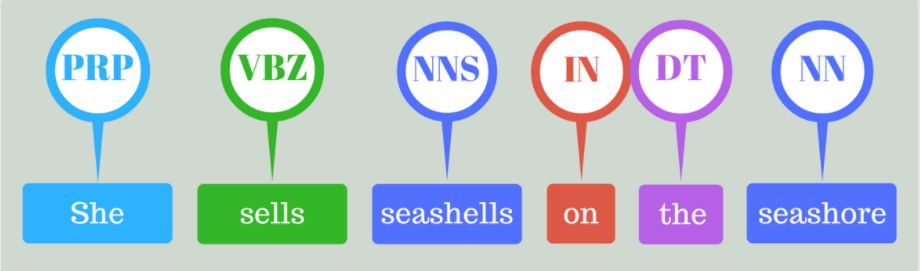
\includegraphics[width=10cm]{img/poslabeling.png}
	\end{center}
	\caption{Voorbeeld van PoS-labeling op de Engelstalige zin "She sells seashells on the seashore". Afbeelding van \textcite{Bilisci2021} }
	\label{fig:pos}
\end{figure}

\begin{figure}[H]
	\begin{center}
		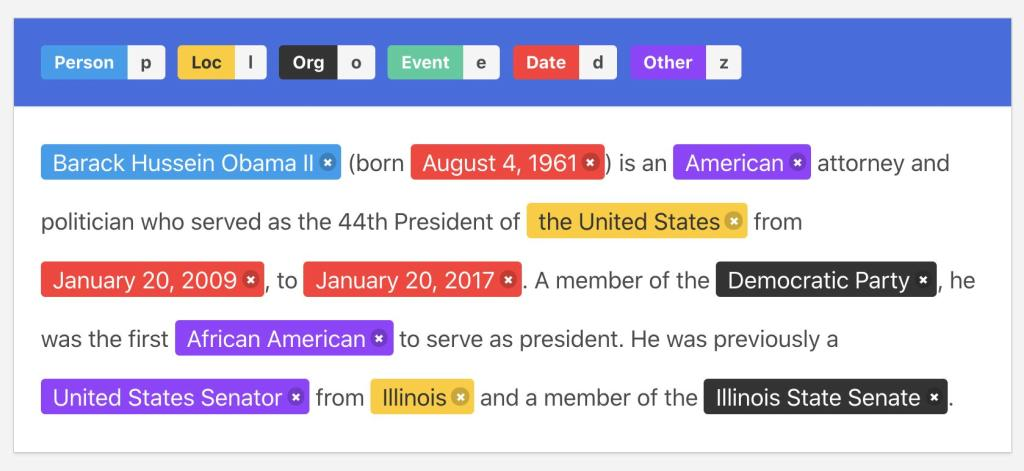
\includegraphics[width=10cm]{img/nerlabeling.jpg}
	\end{center}
	\caption{Voorbeeld van sequence labeling op de Engelstalige zin "She sells seashells on the seashore". Afbeelding van \textcite{Bilisci2021} }
	\label{fig:ner}
\end{figure}


\subsubsection{Prompt engineering}

Large Language Models of LLM's zoals GPT-3, BERT en T5 genereren tekst en karakters op basis van de probabiliteit of waarschijnlijke uitkomst van een gegeven input. Deze modellen maken gebruik van een neuraal netwerk om patronen in de input te herkennen en deze patronen te gebruiken om voorspellingen te doen over de uitvoer \autocite{Liu2020}. Iedereen kan volgens \textcite{McFarland2023} een input of prompt schrijven. Deze tools zoals chatbots zijn ontworpen om zo intuïtief mogelijk te zijn voor een algemeen doelpubliek. Prompt engineering is een steeds belangrijkere vaardigheid die nodig is om effectief te communiceren met LLM’s, zoals ChatGPT \autocite{Harwell2023}.

\begin{figure}
	\begin{center}
			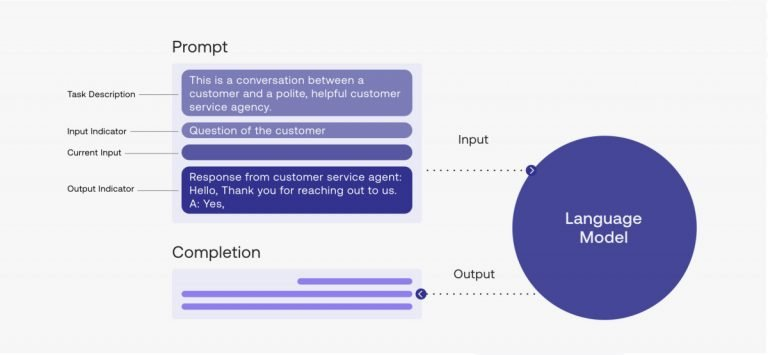
\includegraphics[width=8cm]{img/prompt-engineering-medium.png}
	\end{center}
	\caption{Afbeelding uit \textcite{McFarland2023}. Een illustratie over de werking en begeleiding van prompt engineering bij een taalmodel. }
\end{figure}

Deze prompts werken volgens \textcite{Liu2020} op dezelfde manier als bij mensen en kunnen worden gebruikt om werk te produceren dat is aangepast aan het doel. Text is momenteel het belangrijkste middel van communicatie tussen mens en AI.Een concrete en geoptimaliseerde prompt omvat een concrete scope, duidelijke vraagstelling, specifieke sleutelwoorden, de context en ten slotte gepersonaliseerde keuzes \autocite{McFarland2023}. Bij een zoekopdracht moeten voldoende parameters in de prompt worden opgenomen, zoals het type. Zo niet zal het model te algemeen blijven en mogelijks afwijken van de intentie van de gebruiker. Effectieve AI prompt engineering leidt tot hoogwaardige trainingsgegevens die het AI-model in staat stellen om nauwkeurige voorspellingen en beslissingen te maken \autocite{Liu2020}.

Prompt patterns is samen met prompt engineering naar boven gekomen en is vergelijkbaar met software patterns. Deze patronen zijn herbruikbare oplossingen voor veelvoorkomende problemen in een bepaalde context, waaronder vooral de interactie bij het werken met LLM's. \textcite{White2023} haalt vijf verschillende prompt patterns aan.

\begin{itemize}
\item	Intent-prompts waarbij een LLM een instructie krijgt met een specfiek verwacht antwoord.
\item	Restriction-prompts die het antwoord van een LLM inperkt. Deze pattern is noodzakelijk om een LLM binnen de lijnen te houden.
\item 	Contextualization-prompts verzekeren dat de output van een LLM relevant is. Een context wordt aan de LLM meegegeven.
\item	Expansion/reduction-prompts genereren een output dat beknopt is, maar met voldoende details. 
\end{itemize}

\subsubsection{Traditional en contextual word embeddings}

NLP-systemen en machines moeten woorden, grammatica en nuancering kunnen begrijpen. Embeddings transformeren woorden tot een numerieke representatie, waarop een machine deze representaties kan aanleren om nadien tekst te verwerken. Traditionele word embeddings bouwen een woordenschat op met unieke woorden. De betekenis achter ieder woord wordt niet opgevolgd. Voorbeelden van traditionele word embeddings zijn Word2Vec en Glove.

Contextual word embeddings lossen dit probleem op en houden rekening met de context waarin een woord wordt gebruikt. ELMo en BERT zijn voorbeelden van een model voor contextuele embedding. Deze vorm houdt de semantiek bij van een woord in een bepaalde context en is noodzakelijk wanneer een machine polysemantische woorden in een tekst moet begrijpen. Contextuele word embeddings worden vergkregen uit transformer-gebaseerde modellen. Ze worden verkregen door een volledige zin door te geven aan een pre-trained model.

BERT is een meertalig LLM, getraind op 110 miljoen parameters uit 104 verschillende talen\footnote{https://github.com/google-research/bert/blob/master/multilingual.md#list-of-languages}, waaronder Nederlands. Dit taalmodel kent alternatieven die verderbouwen op het oorspronkelijke BERT-model. Voor de Nederlandse taal zijn er twee, namelijk RobBERT en BERTje. Volgens (..) is RobBERT de krachtigste van de twee modellen, waar BERTje compacter is. Vervolgens bepaalt de \textit{Substitution Ranking} of SR-stap welke vervanging de beste is uit een set van kandidaten. SR gebeurt door gegenereerde substituties op basis van relevantie te rangschikken.

\section{De verschillende soorten tekstvereenvoudiging}

Tekstvereenvoudiging bestaat volgens \textcite{Siddharthan2014} uit vier soorten transformaties: lexicale, syntactische en semantische vereenvoudiging en samenvatten.

\begin{figure}[H]
	\begin{center}
			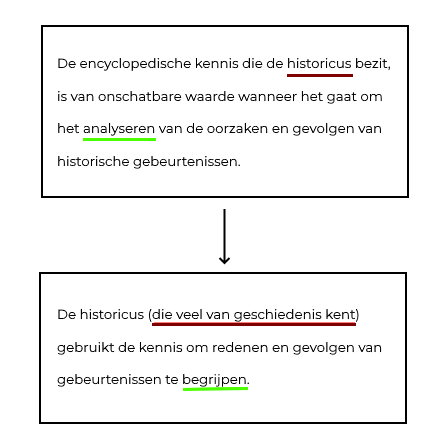
\includegraphics[width=5cm]{img/voorbeeld-manuele-vereenvoudiging.png}
	\end{center}
	\caption{Voorbeeld van tekstvereenvoudiging. Oorspronkelijke tekst uit Historia 5 bron toe te voegen}
\end{figure}

\subsection{Lexicale vereenvoudiging}

Bij \textit{lexical simplification} (LS) of lexicale vereenvoudiging worden complexe woorden vervangen door eenvoudigere synoniemen. Bijvoorbeeld, het woord 'adhesief' wordt vervangen door 'klevend'. \textcite{Kandula2010} haalt twee manieren aan om lexicale vereenvoudiging mogelijk te maken, namelijk het vervangen door een synoniem en het aanmaken of genereren van extra uitleg. De zinsstructuur verandert niet en er is garantie dat de kerninhoud en benadrukking in een tekst identiek blijft. Het doel van lexicale vereenvoudiging is om de moeilijkheidsgraad van de woordenschat in een zin of tekst te verlagen. 

\subsubsection{Complex Word Identification}

\textit{Complex word identification} of CWI is een gesuperviseerde NLP-taak. In een pipeline voor lexicale tekstvereenvoudiging is CWI de eerste stap. Moeilijke woorden of \textit{multi-word expressions} (MWE) in een tekst worden achterhaald  \autocite{Shardlow2013, Gooding2019}. Na CWI kan LS gebruikt worden om deze woorden te vervangen door eenvoudigere synoniemen of om verdere elaboratie te voorzien met behulp van voorbeelden of definities \autocite{Zeng2005, Kandula2010}. CWI is volgens \textcite{Shardlow2013} een cruciale stap, want een lage \textit{recall} van dit component zal een uitvoertekst geven waar moeilijke woorden niet worden vereenvoudigd. Het model zal moeilijke woorden laten staan.

\subsubsection{Substitutiegeneratie en ranking}

Substitutiegeneratie wordt gedaan door synoniemen te zoeken voor een doelwoord in lexicale databanken zoals WordNet, BERT, context2vec, nPIC of OOC. 

\begin{figure}[H]
	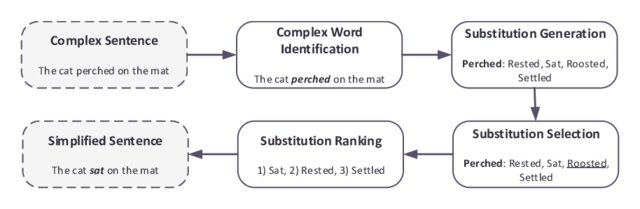
\includegraphics{img/lexical-simplification-pipeline.png}
	\caption{Afbeelding van \textcite{Althunayyan2021}. Deze pipeline wordt in meerdere onderzoeken rond lexicale vereenvoudiging toegepast, zoals \textcite{Paetzold2016, Bingel2018, Bulte2018}}
\end{figure}

% todo FrenLys

\subsection{Syntactische vereenvoudiging}

Syntactische vereenvoudiging verlaagt de leesgraad en complexiteit van een zin door de grammatica en zinsstructuur van een tekst aan te passen. Twee afzonderlijke zinnen kunnen samengevoegd worden tot één eenvoudigere zin. Zo worden complexe of onduidelijke zinsconstructies verminderd, terwijl de inhoud en betekenis van de tekst behouden blijft. Dergelijke transformaties zijn het vereenvoudigen van de syntax of door de zinnen korter te maken. Zinnen worden toegankelijker, zonder de kerninhoud of relevante inhoud te verliezen.

\textcite{Kandula2010} ontwikkelde een toepassing om medische informatie bij beschikbare biomedische bronnen te vereenvoudigen. Dit model verlaagt de leesgraad door syntactische vereenvoudiging op zinniveau toe te passen. Zinnen met meer dan tien woorden worden in het onderzoek als complex beschouwd en worden vereenvoudigd door drie modules. Na deze transformatie kan de oorspronkelijke zin ongewijzigd worden behouden of vervangen worden door twee of meer kortere zinnen. De architectuur van dit model omvat drie onderdelen: een \textit{Part of Speech (PoS) Tagger}, een \textit{Grammar Simplifier} en een \textit{Output Validator}. 

\begin{itemize}
	\item Voor de \textit{PoS Tagger}-fase gebruikten \textcite{Kandula2010} beschikbare functies uit het open-source pakket OpenNLP\footnote{https://opennlp.apache.org/}.
	\item De \textit{Grammar Simplifier} module splitst de lange zin in twee of meer kortere zinnen door POS-patronen te identificeren en een set transformatieregels toe te passen.
	\item De \textit{Output Validator} module controleert de output van de Grammar Simplifier op grammatica en leesbaarheid.
\end{itemize}  

\subsection{Tekstvereenvoudiging automatiseren}

Geautomatiseerde tekstvereenvoudiging is geen nieuw concept. Volgens onderzoeken van \textcite{Canning2000, Siddharthan2006} waren de eerste aanpakken op geautomatiseerde tekstvereenvoudiging gebouwd op rule-based modellen. Deze modellen bewerken de syntax door zinnen te splitsen, te verwijderen of de volgorde van de zinnen in een tekst aan te passen. Lexicale vereenvoudiging kwam hier niet aan de pas. Enkel bij recentere onderzoeken van \textcite{Coster2011, Bulte2018} werd het duidelijk hoe lexicale en syntactische vereenvoudiging gecombineerd kon worden.

\section{Samenvatten}

Lexicale, conceptuele en/of syntactische vereenvoudiging van teksten leidt niet altijd tot een kortere tekst. Technologieën zoals full-text-search en gepersonaliseerde informatiefiltering benadrukken het belang van gebruikersgerichte samenvatting. De architectuur van een samenvattingssysteem omvat drie fases: analyse van de brontekst, identificatie van kernpunten en het samenvoegen van de punten tot één uitvoertekst. Teksten machinaal samenvatten is geen nieuw concept en kan op twee manieren gebeuren: extraherend en abstraherend \autocite{Hahn2000, Dubay2004}.

% Teksten vereenvoudigen met lexicale, conceptuele en/of syntactische vereenvoudiging biedt geen garantie dat de tekstinhoud korter zal worden. Bij de drie soorten vereenvoudiging wordt er initieel enkel per zin gekeken. De vereenvoudiging houdt geen rekening met voorafgaande of opvolgende zinnen \autocite{Dubay2004}. Teksten machinaal samenvatten is geen nieuw concept. Het onderzoek van \textcite{Hahn2000} onderzoekt hoe teksten automatisch samengevat kunnen worden. Dit onderzoek haalt onder meer twee aanpakken aan hoe een machine teksten kan samenvatten, namelijk extraherend en abstraherend. Daarnaast reikt \textcite{Hahn2000} drie manieren aan welke inhoud er zeker in de samengevatte versie moet op te merken zijn.

% Generiek en gebruikersgerichte samenvatting
% Verder haalt \textcite{Hahn2000} ook het onderscheid tussen een generieke en een gebruikersgerichte samenvatting. Een generieke samenvatting staat niet stil bij speciale noden of interesses van de eindgebruiker. Daarnaast houdt een gebruikersgerichte samenvatting wel rekening met sleutelwoorden of thema's in een tekst. \textcite{Hahn2000} haalt aan dat technologieën zoals \textit{full-text-search} en gepersonaliseerde informatiefiltering het belang van gebruikersgerichte samenvatting naar voor duwen. \textcite{Hahn2000} omschrijft de architectuur van een samenvattingssysteem aan de hand van drie fases. Allereerst wordt de brontekst geanalyseerd. Daarna worden de \textit{salient points} of kernpunten in een tekst aangeduid. Deze punten zijn zinnen of tokens. Ten slotte worden de punten samengevoegd tot één uitvoertekst. De nadruk is verschillend per samenvattingsmethode.

\subsection{Extraherend samenvatten}

Bij extraherende samenvatting worden de belangrijkste zinnen gemarkeerd en opnieuw neergeschreven, maar dit kan leiden tot onsamenhangende uitvoertekst. Om de kernzinnen te achterhalen, zijn zes kenmerken volgens \textcite{Khan2014} essentieel, namelijk woordfrequentie, de plaats van een zin in de tekst, de \textit{cue method}, titels, de lengte van de zin, de gelijkenissen tussen de zin en de rest van het document, \textit{proper nouns} woordgebruik en ten slotte de afstand tussen \textit{text units} waarin entiteiten voorkomen. \textcite{Verma2020} onderzocht verschillende manieren om een tekst extraherend samen te vatten, waaronder graafgebaseerd extraherend samenvatten, maximal marginal relevance en meta-heuristic-gebaseerd samenvatten.

% Bij deze vorm worden de belangrijkste zinnen gemarkeerd en vervolgens opnieuw neergeschreven.  Dit is het equivalent van handmatig zinnen markeren en vervolgens op een blanco papier neerschrijven. Het nadeel hiervan is dat de uitvoertekst niet samenhangend kan zijn na het samenvatten. Kernzinnen achterhalen gebeurt bij geautomatiseerde samenvatting met zes features volgens \textcite{Khan2014}, namelijk de woordfrequentie, de plaats van een zin in de tekst, de \textit{cue method} of een woord dat de kerngedachte van een paragraaf benadrukt, titels, de lengte van de zin, de gelijkenissen tussen de zin en de rest van het document, het gebruik van \textit{proper nouns} en ten slotte de afstand tussen \textit{text units} waarin entiteiten voorkomen. De uitvoertekst kan coherentie en de oorspronkelijke structuur ontbreken. Dit maakt de uitvoertekst minder aangenaam om te lezen. \textcite{Verma2020} onderzocht de verschillende manieren waarop een tekst extraherend kan worden samengevat. Zij halen drie grote componenten aan, namelijk:

\subsubsection{Graafgebaseerd extraherend samenvatten}

De graafgebaseerde techniek van extraherend samenvatten vertegenwoordigt een document als een graaf van zinnen en gebruikt algoritmen om de belangrijkste zinnen te bepalen en redundantie te vermijden \autocite{Parveen2015}. Dit kan volgens \textcite{Parveen2015} zowel voor lange wetenschappelijke artikelen als korte nieuwsartikelen goede resultaten opleveren, vooral als coherentie en positionele informatie worden opgenomen. Het compacte SqueezeBERT-model kan ook worden ingezet voor real-time samenvatting, als een interessant alternatief op het grotere BERT-model, met bijna de helft van de grootte en minimale afbreuk in prestaties. Beide methoden kunnen de prestaties van NLP-downstream taken verbeteren \autocite{AbdelSalam2022}.

% Graafgebaseerd extraherend samenvatten is een techniek die een document voorstelt als een graaf, waarbij de knopen zinnen en bogen de relatie tussen de zinnen representeren. Deze algoritmen achterhalen de kernzinnen in een tekst. Bijvoorbeeld kan het PageRank-algoritme, dat vaak wordt gebruikt voor het rangschikken van webpagina's in zoekmachines, worden gebruikt om de zinnen in de grafiek te rangschikken op basis van hun belangrijkheid.

% \textcite{Parveen2015} raadt een graafgebaseerd systeem aan voor \textit{unsupervised learning}. Belangrijke zinnen worden met een lokaal minimum bepaald, alsook wordt redundantie vermeden. Deze methode kan significante resultaten opleveren bij het ophalen van kernzinnen uit zowel lange wetenschappelijke artikelen als korte nieuwsartikelen. Daarnaast vermeldt \textcite{Parveen2015} dat het systeem beter presteert wanneer coherentie wordt opgenomen en gecombineerd wordt met positionele informatie. % In toekomstig werk is \textcite{Parveen2015} van plan om meer taalkundige informatie in de entiteitsgrafiek op te nemen en beoordelingen van domeinexperts te verkrijgen om te zien of de redactiesamenvattingen als gouden samenvattingen kunnen worden gebruikt voor evaluatie.

% \textcite{AbdelSalam2022} voerden een vergelijkend onderzoek uit rond SqueezeBERT en BERT. De compacte architectuur van SqueezeBERT kan ingezet worden voor real-time samenvatting. Dit is volgens \textcite{AbdelSalam2022} een interessant alternatief op het BERT-model. In vergelijking heeft de voorgestelde SqueezeBERT slechts ongeveer 62 miljoen parameters, terwijl het prestatieniveau nog steeds boven de 90\% van het BERT-baseline model blijft. De evaluatie gebeurde aan de hand van de ROUGE-score. De onderzoekers besluiten dat SqueezeBERT een goed alternatief is, vooral door het trainen met bijna de helft van de grootte van het oorspronkelijke model en minimale afbreuk in de prestaties bij het samenvatten. Daarnaast kan het gebruik van efficiënte netwerken, zoals \textit{grouped convolutional layers}, de NLP-downstream taken verbeteren. 

% \textcite{AbdelSalam2022} haalt verder aan dat er potentie is voor een productieversie van een SqueezeBERT-samenvatter, die minder parameters heeft dan DistilBERT met ongeveer 20\% en dezelfde ROUGE-1 score behoudt, terwijl het iets hogere ROUGE-2 en ROUGE-L scores behaalt. Hoewel de SqueezeBERT en DistilBERT iets lagere scores produceren in vergelijking met het BERT-baseline model, heeft SqueezeBERT als voordeel dat het minder trainingstijd en minder parameters heeft dan het baseline model met ~48,44\%. 

\subsubsection{Maximal Marginal Relevance}

Traditionele samenvattingssystemen zijn gebaseerd op de architectuur van \textcite{Carbonell1998}, die gebruik maakt van de maximaal marginale relevantiescore (MMR) om de relevantie en diversiteit van gemarkeerde zinnen te bepalen. MMR zorgt ervoor dat de geselecteerde zinnen niet te veel overlappen in inhoud en relevantie. Onderzoekers hebben voorgesteld om het gulzige zoekalgoritme van MMR te vervangen door een globaal optimale formulering, wat een betere samenvatting oplevert, maar wel meer rekenkracht en tijd vereist. Evaluaties van deze methode tonen echter significant betere resultaten \textcite{McDonald2007, Lin2010}.

% Traditionele extraherende samenvattingssystemen bouwen verder op de door \textcite{Carbonell1998} ontworpen architectuur. Deze architectuur gebruikt een maximaal marginale relevantiescore of MMR. Deze architectuur houdt rekening met de diversiteit en de relevantie van de gemarkeerde zinnen. De relevantie van een zin in een tekst wordt bepaald door de mate waarin het taalmodel de belangrijkste informatie overbrengt van de tekst waarvan het afkomstig is. Om diversiteit aan tekstinhoud te waarborgen, wordt er gekeken naar de mate waarin de geselecteerde zinnen verschillen van de eerder geselecteerde zinnen in de samenvatting. Als een zin relevant is maar qua inhoud te veel overlapt met de eerder geselecteerde zinnen, dan heeft deze minder kans om in de geëxtraheerde samenvatting opgenomen te worden. Deze score kan doorgaans berekend worden met KeyBERT\footnote{https://maartengr.github.io/KeyBERT/api/mmr.html}.

% Extraherend samenvatten met de MMR-methode is de methode bij uitstek voor ML-toepassingen. Onderzoekers bouwen verder op de architectuur die beschreven staat in \textcite{Carbonell1998}. In \textcite{McDonald2007} stelt de onderzoeker voor om het gulzige zoekalgoritme van MMR te vervangen door een globaal optimale formulering, waarbij het MMR-framework wordt uitgedrukt als een knapzakprobleem of NP-volledig probleem. Daarmee wordt er gewezen naar een \textit{integer linear programming} (ILP) \textit{solver} die gebruikt kan worden om de wiskundige functie van MMR te maximaliseren. De MMR-methode hield voordien enkel rekening met relevantie en diversiteit, maar niet met de optimale combinatie van zinnen die in een samenvatting moet worden opgenomen. De aanpak van \textcite{McDonald2007} vereist echter meer rekenkracht en tijd dan de standaard MMR-methode, maar het experiment van \textcite{McDonald2007} haalde wel aan dat deze methode leidde tot significant betere resultaten. \textcite{Lin2010} evalueerde dit MMR-algoritme. Bij de evaluatie van deze architectuur benadrukte zij de significant betere resultaten. 

\subsubsection{Metaheuristiek-gebaseerd}

Metaheuristische samenvatting is een benadering die gebruik maakt van optimalisatie-algoritmen zoals genetische algoritmen, simulated annealing en zwermoptimalisatie om de belangrijkste zinnen in een tekst te vinden. Volgens \textcite{Premjith2015, Verma2020} zoeken deze algoritmen naar de beste combinatie van zinnen om de kerninformatie in de tekst te bevatten. De evaluatiefunctie kan verschillende criteria bevatten, zoals zinslengte, relevantie en verbanden, aldus \textcite{Rani2021}. Een beperking van deze methode is dat deze vaak vastloopt in een lokaal optimum en geen extremen of steilere hellingen op een zoekruimte aangeeft. Om de convergentie te versnellen, is het nodig om een optimalisatiestrategie te gebruiken die gebaseerd is op gradiënten.

% Metaheuristieke samenvatting maakt gebruik van metaheuristieke optimalisatie-algoritmen zoals genetische algoritmen, \textit{simulated annealing} of zwermoptimalisatie om de belangrijkste zinnen in een tekst te achterhalen. Deze algoritmen zoeken volgens  naar de beste combinatie van zinnen die de belangrijkste informatie in de tekst bevatten. De evaluatiefunctie in metaheuristieke samenvattingsalgoritmen kan gebaseerd zijn op verschillende criteria, zoals zinslengte, -relevantie en -verbanden.  benadrukt dat teksten samenvatten met een metaheuristieke methode regelmatig vastraakt in een lokaal optimum. Dit is een tekortkoming op andere methoden. Daarnaast wijst het onderzoek uit aan dat metaheuristieke methoden geen \textit{steepness} of extremen op een \textit{search space behaviour} aanduiden. Om de convergentie aanzienlijk te versnellen, moet er gebruik worden gemaakt van een optimalisatiestrategie gebaseerd op gradiënten. 

% gradienten: (een wiskundig concept dat de richting van de snelste toename aangeeft)
% convergentie: (het proces waarbij het algoritme naar de juiste oplossing toewerkt) -- Hierdoor wordt het algoritme efficiënter en sneller uitgevoerd.

\subsubsection{Experimenten over extraherend samenvatten}
% \subsubsection{title}

% todo https://medium.com/jatana/unsupervised-text-summarization-using-sentence-embeddings-adb15ce83db1 --> voorbeeld van een pipeline

\textcite{McKeown1999} voerden experimenten uit op extraherende samenvattingen van nieuwsartikelen. De resultaten wijzen erop dat deze vorm vatbaar is op vooroordelen of \textit{bias} van de auteur. De zinnen worden genomen zoals ze zijn. \textcite{Hahn2000} bouwde verder op dit experiment. Zij voerden een experiment uit met een mix van \textit{knowledge-rich} en \textit{knowledge-poor} methoden, met significant positieve resultaten tot gevolg. De nadruk bij extraherend samenvatten ligt in het kiezen van de \textit{salient text units}. Deze punten zijn typisch in de vorm van zinnen. Er is nood aan een manier om de lexicale en statistische relevantie van een zin te kunnen aanduiden. Hiervoor haalt \textcite{Hahn2000} twee manieren aan:

\begin{itemize}
	\item Een lineair gewicht model. Iedere teksteenheid wordt gewogen op factoren zoals de \textit{location weight} en het aantal voorkomens.
	\item Een gewicht model op basis van de statistische opvallendheid van een eenheid. Zo wordt er rekening gehouden met de aanwezigheid van een woord in (sub)titels.
\end{itemize}

% resultaten lineair gewicht model
% resultaten statistische opvallendheid

\textcite{Nallapati2017} wilden de nauwkeurigheid van deze modellen overbruggen. Dit doen ze met \textit{SummaRuNNer}\footnote{https://github.com/hpzhao/SummaRuNNer}, een oplossing voor het extraherend samenvatten van teksten met een neuraal netwerk. De toepassing werd opgebouwd met PyTorch in  en bestaat uit een combinatie van drie modellen: een recurrent neuraal netwerk, een convolutioneel recurrent neuraal netwerk en een \textit{hiërarchical attention network}.

\subsection{Abstraherend samenvatten}

Er zijn twee manieren om een tekst abstraherend samen te vatten: semantisch en structuurgebaseerd. De structuurgebaseerde benadering gebruikt regels om belangrijke informatie in de tekst te vinden en kan leiden tot samengevatte zinnen met lage linguïstische kwaliteit en grammaticale fouten. De semantisch-gebaseerde benadering gebruikt de betekenis van de tekst om korte en duidelijke samenvattingen te maken met minder redundante zinnen en betere linguïstische kwaliteit, hoewel een extra parsingfase nodig kan zijn. \textcite{Cao2022} heeft verder onderzoek gedaan naar deep learning methoden om automatisch abstraherende samenvattingen te genereren. Deep learning-modellen zoals RNN's, CNN's en Seq2Seq kunnen worden gebruikt voor abstraherend samenvatten door de betekenis van de tekst te begrijpen en belangrijke informatie over te brengen \autocite{Suleiman2020}. Het Pegasus-model, beschreven in \textcite{Zhang2020}, maakt gebruik van pre-trained modellen voor samenvatting met NLP en handelt gap-zinnen af, en is getraind en beoordeeld op verschillende soorten samenvattingstaken. LED of Longformer Encoder-Decoder is specifiek ontworpen om lange documenten te verwerken, waardoor het geschikt is voor het samenvatten van langere wetenschappelijke artikelen. % https://www.hindawi.com/journals/mpe/2020/9365340/

% \textit{Deep learning} voor abstraherend samenvatten kan met verschillende modellen zoals RNN’s (terugkerende neurale netwerken), CNN’s (convolutionele neurale netwerken) en sequence-to-sequence (Seq2Seq) modellen. Deze modellen kunnen leren om samenvattingen te maken door de betekenis van de tekst te begrijpen en nieuwe tekst te maken die de belangrijkste informatie overbrengt \autocite{Suleiman2020}. Om een abstraherende samenvatting met deep learning op te bouwen bestaan er verschillende modellen. Het Pegasus-model beschreven in \textcite{Zhang2020} handelt \textit{gap-sentences} af met pre-trained models voor samenvatting met NLP.  Dit model werd getrained en beoordeeld op samenvattingstaken zoals emails, patenten, rekeningen en ook wetenschappelijke artikelen \autocite{Zhang2020}.

\subsection{Hybride samenvatten}

In het best denkbare geval wordt abstraherende en extraherende samenvatting gecombineerd volgens \textcite{Hsu2018, Huang2019}. Zo omvat een pipeline voor hybride samenvatting twee onderdelen: een \textit{content selection} fase waarin de kernzinnen met extraherende samenvatting worden opgehaald en \textit{paraphrasing}-fase waarbij de gemarkeerde kernzinnen abstraherend worden samengevat. 

\subsection{Evaluatie}

Samenvattingen van lange documenten handmatig beoordelen vergt tijd en voldoende planning van een mens \autocite{Nenkova2004}. Met behulp van een vooraf geschreven samenvatting als referentietekst zorgen twee metrieken voor ondersteuning om een samenvatting automatisch te laten beoordelen. Samenvattingen beoordelen kan ook zonder referentietekst, al moeten verschillende factoren worden opgevolgd.

\subsubsection{Evaluatie met referentieteksten}

Bij het vergelijken van teksttransformaties worden vaak BLEU en ROUGE gebruikt, twee metrieken die de gelijkenis tussen machine-gegenereerde en referentieteksten meten gebaseerd op exacte \textit{token matches}. ROUGE volgens \textcite{Lin2004} is recall-gebaseerd en houdt geen rekening met synoniemen, maar er zijn ROUGE-modellen die dit wel doen. ROUGE-2 van \textcite{Ganesan2018} voorziet dictionaries van synoniemen, zodat er rekening wordt gehouden met synonieme zinnen. ROUGE-G van \textcite{ShafieiBavani2018} gebruikt graafalgoritmen om lexicale en semantische matching mogelijk te maken. BLEU is precision-gebaseerd is en een \textit{brevity penalty} introduceert om te korte teksten te voorkomen. Er zijn Python-bibliotheken beschikbaar voor zowel ROUGE\footnote{https://github.com/pltrdy/rouge} als BLEU\footnote{https://github.com/neural-dialogue-metrics/BLEU}.

\subsubsection{Evaluatie zonder referentieteksten}

Een samengevatte tekst beoordelen zonder een referentietekst vereist volgens \textcite{Steinberger2009} meer subjectiviteit en menselijke betrokkenheid dan met een referentietekst. Deze soort kan handmatig gebeuren, maar ook semi-automatisch. De type tekst, de lengte en de complexiteit van de oorspronkelijke tekst zijn factoren die in acht moeten worden genomen bij het beoordelen van de samengevatte tekst. Daar moet er worden gekeken naar het doelpubliek en het formaat. De tekst- en inhoudskwaliteit van de samengevatte tekst moet worden beoordeeld. De tekstkwaliteit is de grammaticale correctheid, niet-redundantie van zinnen en woordenschat en coherente structuur \autocite{McCombes2022}. De inhoudskwaliteit wijst op de informatie dat wordt opgenomen in de samengevatte tekst. Dit omvat de relevantie met de doelgroep bij kern- en bijzaken of misleidende informatie door een misinterpretatie van het systeem \autocite{McCombes2022}.


\subsection{Tekstvereenvoudigingstechnieken voor scholieren met dyslexie.}

In het onderzoek van \textcite{Bingel2018} wordt een systeem beschreven voor lexicale tekstvereenvoudiging, waarbij gebruik wordt gemaakt van een embeddings-gebaseerde aanpak voor substitution generation en een gesuperviseerd SR-model voor de selectie van synoniemen. Het systeem kan gepersonaliseerd worden op basis van gebruikersfeedback en maakt gebruik van een seed-dataset van complex-simple overeenkomsten. Het onderzoek van \textcite{DeBelder2010} richt zich op tekstvereenvoudiging voor kinderen van acht tot twaalf jaar en maakt gebruik van een methode voor lexicale en syntactische vereenvoudiging, terwijl \textcite{Bulte2018} een pipeline ontwikkelt om moeilijke woorden naar simpele synoniemen te vervangen, met behulp van een lexicale databank en LLM's.

% \textcite{Bingel2018} beschrijft een systeem voor dat gericht is op lexicale tekstvereenvoudiging en een embeddings-gebaseerde aanpak voor substitution generation. Tijdens de substitution selection maakt het systeem gebruik van een ongesuperviseerde boundary ranker om de synoniemen te filteren. De geselecteerde synoniemen worden vervolgens gerangschikt met behulp van een gesuperviseeerd SR-model. Daarnaast is het systeem in staat om het model te personaliseren op basis van gebruikersfeedback en maakt het gebruik van een seed-dataset van complex-simple overeenkomsten. Deze overeenkomsten houden rekening met de context van een woord in een zin en helpen bij de initiële vereenvoudiging van teksten. Alle gebruikersinformatie wordt met een PostgreSQL databank bijgehouden. Gebruikersinformatie wordt gekoppeld aan de demografische informatie informatie, om zo de ideale uitvoertekst te kunnen genereren. 

% Het onderzoek van \textcite{DeBelder2010} richt zich op tekstvereenvoudiging voor kinderen van acht tot twaalf jaar. Het onderzoek zet een methode op voor lexicale en syntactische vereenvoudiging. \textcite{Bulte2018} werkte het aspect rond lexicale vereenvoudiging verder uit. Het resultaat van dit onderzoek was een \textit{pipeline} ontworpen om moeilijke woordenschat naar simpele synoniemen te vervangen. Eerst ging de tekstinhoud door een \textit{preprocessing}-fase, samen met het uitvoeren van WSE. Daarna werd de moeilijkheidsgraad van ieder token overlopen. De moeilijkheidsgraad is gebaseerd op de frequentie in SONAR500\footnote{https://taalmaterialen.ivdnt.org/download/tstc-sonar-corpus/} een corpus met eenvoudige Nederlandstalige woorden, en ook de Wablieft-corpus, een archief van nieuwsartikelen in eenvoudig Nederlands. Synoniemen werden teruggevonden met Cornetto\footnote{https://github.com/emsrc/pycornetto}, een lexicale databank met Nederlandstalige woorden, samen met een \textit{reverse lemmatization} fase. Lexicale vereenvoudiging is ingewikkeld wanneer er geen eenvoudigere synoniemen zijn. In dat geval blijft een moeilijk woord voor wat het is. Voor deze toepassing maakten de onderzoekers gebruik van LLM's samen met Wikipedia annotaties. Deze annotaties bevestigden of de gegeven informatie correct is. De resultaten van deze toepassingen vallen in lijn met andere huidige toepassingen van hun soort. De onderzoekers benadrukken dat deze toepassing ook voor andere doelgroeppen met een lagere leesgraad kunnen dienen, zoals L2-lezers.

\begin{figure}[H]
	\begin{center}
			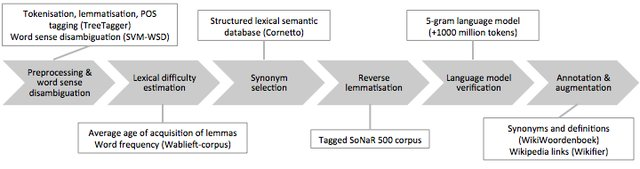
\includegraphics[width=9cm]{img/dutch-simplification-dyslexia-pipeline.png}
	\end{center}
	\caption{Afbeelding uit \textcite{Bulte2018}. Deze pipeline omvat de stappen die de toepassing aflegt. }
\end{figure}

\begin{figure}[H]
	\begin{center}
			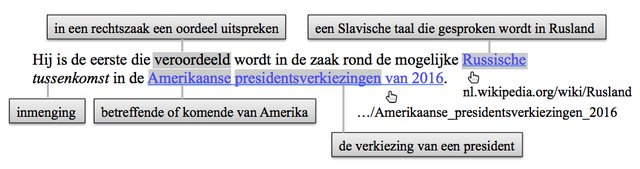
\includegraphics[width=9cm]{img/dutch-simplification-dyslexia-example.png}
	\end{center}
	\caption{Afbeelding uit \textcite{Bulte2018}. TODO}
\end{figure}


Al zijn er onderzoeken over lexicale, syntactische en semantische vereenvoudiging voor kinderen en scholieren met dyslexie, het aantal onderzoeken over samenvatten voor deze doelgroep is schaars. Zoals eerder aangehaald is er wel onderzoek gedaan naar de verschillende manieren om een tekst samen te vatten, maar er is geen toepassing of onderzoek dat dit concreet uitwerkt. 

\subsection{Conclusie}

Wetenschappelijke artikelen volgen een gelijke structuur. De inhoud in PDF- of afbeeldingvorm vergt voldoende cleaning-fasen. Het beoordelen van de samenvatting op basis van een referentietekst met de ROUGE-metriek wordt aangeraden, al kan deze beoordeling niet enkel machinaal gebeuren. Daarnaast is er input en bijsturing nodig van de mens omtrent een samenvatting op maat en de grammaticale, lexicale en semantische correctheid. Tools gericht op het lexicaal en adaptief vereenvoudigen van teksten voor kinderen en scholieren met dyslexie zijn reeds uitgewerkt. Methoden om menselijke en grammatisch correcte samenvatting op te bouwen zijn reeds beschikbaar. 

\section{Valkuilen en uitdagingen voor AI-ontwikkelaars bij tekstvereenvoudiging met AI}

AI en ML zijn volop in groei. NLP gebruikt AI en ML om menselijke taal te verwerken, terwijl NLU deze technologieën gebruikt om menselijke taal te begrijpen. Hoewel deze technologieën veelbelovend zijn, moeten AI-ontwikkelaars rekening houden met veelvoorkomende en genegligeerde uitdagingen en valkuilen \autocite{Sciforce2020, Roldos2020, Khurana2022}. Deze sectie beantwoordt de volgende onderzoeksvraag: "Met welke valkuilen bij taalverwerking met AI moeten ontwikkelaars rekening houden?"

\subsection{Uitdagingen voor softwarebedrijven}

NLP- en NLU-toepassingen behoren tot de duurste om te ontwikkelen, wat een obstakel kan vormen voor veel IT-professionals. Het gebrek aan NLP-expertise, de kwaliteit en kwantiteit van data, de integratie en deployment van modellen en de transparantie van modellen zijn allemaal factoren die bijdragen aan deze hoge kosten \autocite{IBM2022}. Software-ontwikkelaars verkiezen volgens  voor \textit{black-box} modellen bij de ontwikkeling en finetuning van een NLP-toepassing met AI. Al is het verschil qua nauwkeurigheid minimaal, de afweging wordt gemaakt bij de transparantie van het model. Na een transformatie wordt er niet aangegeven waarom specifieke transformaties werden uitgevoerd, bijvoorbeeld het vervangen van een woord door een eenvoudiger synoniem. White-box taalmodellen zijn er in schaarse hoeveelheden \autocite{Punardeep2020}. 

% Volgens het jaarlijks rapport van IBM behoren NLP en NLU-toepassingen tot de duurste soort om te ontwikkelen. Ongeveer 54\% van de bevraagde IT-professionals vond de bijhorende kosten een obstakel bij het starten van de ontwikkeling voor NLP-toepassingen. Professionals halen verschillende pijlers aan, waaronder de kwaliteit en kwantiteit van de data, het trainen van de data, het gebrek van NLP-experten, de integratie en deployment van de taalmodellen en ten slotte de transparantie van het model. Gespecialiseerde modellen zijn use-case afhankelijk wat ze niet voor iedere toepassing bruikbaar maakt. Als oplossing kunnen softwarebedrijven partnerships afsluiten, investeren in NLP-talent, klein starten en stelselmatig opschalen, cloud-gebaseerde oplossingen aanreiken of de transparantie van een model benadrukken in hun specifieke toepassing . Software-ontwikkelaars verkiezen volgens  voor \textit{black-box} modellen bij de ontwikkeling en finetuning van een NLP-toepassing met AI. Al is het verschil qua nauwkeurigheid minimaal, de afweging wordt gemaakt bij de transparantie van het model. Na een transformatie wordt er niet aangegeven waarom specifieke transformaties werden uitgevoerd, bijvoorbeeld het vervangen van een woord door een eenvoudiger synoniem. White-box modellen zijn er in schaarse hoeveelheden. 

\subsection{Ambiguïteit, synoniemen en homoniemen}

Homoniemen kunnen volgens \textcite{Roldos2020} problemen veroorzaken bij sequence labeling of het labelen van tokens in een doorlopende tekst. Bijvoorbeeld bij het woord ‘bank’ is het niet duidelijk voor de machine of het gaat over de geldinstelling of het meubel. Word Sense Disambiguation (WSD), PoS-tagging en contextual embeddings kunnen de betekenis van een woord achterhalen op basis van de context \autocite{Eisenstein2019, Liu2020}. Het gebruik van synoniemen en antoniemen in NLP-systemen kan verbeterd worden door het gebruik van candidate generation en synonym detection, en meertalige transformers zoals BERT bieden een oplossing voor het gebrek aan niet-Engelstalige toepassingen \autocite{Dandekar2016, Roldos2020}.

% Homoniemen kunnen echter roet in het eten gooien. Volgens heeft een machine moeite om de context van homoniemen te achterhalen. Bijvoorbeeld bij het woord ‘bank’ is het niet duidelijk voor de machine of het gaat over de geldinstelling of het meubel. \textit{Word Sense Disambiguation} of WSD achterhaalt de betekenis van een woord op basis van de context waarin een woord gebruikt wordt \autocite{Eisenstein2019}. Deze taak is nodig binnen NLP om rekening te houden met homoniemen. WSD implementeren kan dictionary-gebaseerd, gesuperviseerde, semi-gesuperviseerd of niet-gesuperviseerd. PoS-tagging kan dit probleem aanpakken volgens \textcite{Liu2020} als een oplossing op dit probleem, samen met het gebruik van contextual embeddings. Spacy biedt een sense2vec\footnote{https://github.com/explosion/sense2vec} aan.

% Bij het bouwen van NLP-systemen moeten zo veel mogelijke betekenissen en synoniemen van een woord worden opgenomen. Tekstanalysemodellen zijn niet foutloos, maar deze zullen synoniemen beter begrijpen als deze voldoende en relevante trainingsgegevens ontvangen \autocite{Roldos2020}. \textcite{Dandekar2016} reikt twee methoden aan: \textit{candidate generation} door gebruik te maken van word embeddings, historical user data of lexicale synoniemen. Dit kan ook gesuperviseerd met \textit{synonym detection}. Aanvullend kunnen antoniemen volgens \textcite{Dandekar2016} op eenzelfde manier worden achterhaald met NLP ML.

% Het onderzoek van \textcite{Sciforce2020} haalt aan dat het merendeel van NLP-toepassingen Engelstalige invoer gebruikt. Niet-Engelstalige toepassingen zijn zeldzaam. De opkomst van taalmodellen getrained op meertalige datasets en die meertalige transformers gebruiken, zoals BERT, biedt een oplossing op dit probleem en dempt de impact op ambiguïteit. \autocite{Roldos2020} % De taalmodel vertaalt eerst de oorspronkelijke tekst naar de gewenste taal, voordat de tekst wordt herwerkt. BERT maakt volgens  gebruik van meertalige transformers, wat de impact op verwarring kan dempen.

\subsection{Paternalisme en ethische overwegingen}

Tekstvereenvoudiging is bedoeld om gelijke kansen te bieden aan iedereen, maar ethische overwegingen en bewustzijn van de behoeften van de eindgebruiker zijn belangrijk bij het ontwikkelen van adaptieve tekstvereenvoudigingstoepassingen, zoals beschreven in onderzoeken van \textcite{Niemeijer2010, Xu2015, Gooding2022}. De eindgebruiker moet de keuze hebben om te kiezen welke delen van de tekst vereenvoudigd moeten worden, wat kan worden bereikt door synoniemen te kiezen of zinnen te markeren die moeilijk te begrijpen zijn.

% De doelstelling van ondersteunende toepassingen is om gelijke kansen te bieden aan iedere doelgroep. Tekstvereenvoudiging transformeert de oorspronkelijke tekst naar een tekst met een simpelere syntax, kortere zinnen, verminderde lexicale en semantische complexiteit en gereduceerd aantal zinnen. Volgens \textcite{Niemeijer2010} zijn de ethische overwegingen die samenhangen met tekstvereenvoudiging niet gemakkelijk te scheiden van de gebruikte technologie om het resultaat te bereiken. Het onderzoek van \textcite{Xu2015, Gooding2022} halen pijlers aan waarmee ontwikkelaars en softwarebedrijven rekening moeten houden bij de ontwikkeling van adaptieve en ondersteunende software voor tekstvereenvoudiging. Ontwikkelaars moeten zich meer bewust worden van de behoeften en verwachtingen van de eindgebruiker bij het ontwikkelen van een tekstvereenvoudigingstoepassing. Haar onderzoek benadrukt de paternalistische of afhankelijke aard van assisterende toepassingen. Tekstvereenvoudiging omvat vier transformaties, maar niet iedere transformatie is vereist voor iedere gebruiker. Een adaptieve tekstvereenvoudigingstoepassing moet de eindgebruiker een keuze aanbieden om aan te passen wat vereenvoudigd wordt, afhankelijk van specifieke behoeften. Om dit probleem op te lossen, is het belangrijk om de eindgebruiker, in dit geval scholieren met dyslexie in het derde graad middelbaar onderwijs, de keuze te geven. Zoals beschreven in \textcite{Gooding2022}, zijn er verschillende mogelijkheden. Bijvoorbeeld, de eindgebruiker moet de mogelijkheid hebben om te kiezen welke synoniemen de tekst lexicaal zullen aanpassen. Een alternatieve aanpak voor syntactische vereenvoudiging is om de scholier zelf zinnen te laten markeren die moeilijk te begrijpen zijn, zodat het systeem alleen de door de eindgebruiker aangegeven zinnen vereenvoudigt.

\subsection{Valkuilen bij prompt engineering}

% Iedereen is in staat om een conversatie met een chatbot op te bouwen. Het gebruik van de API voor een doelgericht en doordacht antwoord vergt echter planning bij de ontwikkelaar. \textcite{Miszczak2023} waarschuwt voor 'garbage-in garbage-out'. De kwaliteit van de input kan de kwaliteit van de output bepalen. \textcite{Jiang2023} benoemt de misopvatting bij de intentie van de gebruiker als de voornaamste uitdaging voor een taalmodel dat input vereist. Volgens Jiang kan dit te wijten zijn aan de gebruiker die een onvolledige prompt of een prompt met onvoldoende context op een concreet antwoord schrijft. Daarnaast kan een gebrek aan trainingsdata ook aan de oorzaak liggen van een onnauwkeurige uitvoertekst of bias in het taalmodel. Andere factoren die \textcite{Miszczak2023} aanhaalt, zijn de afwisselende probabiliteit van de outputtekst en de meegegeven parameters die het model beïnvloeden, zoals de temperature dat de creativiteit van het model beïnvloedt. Als oplossing kan de prompt als een conditionele expressie worden opgebouwd, zodat het taalmodel enkel met zekerheid een antwoord teruggeeft.

Het bouwen van een conversatie met een chatbot is voor iedereen mogelijk, maar het vereist doordachte input en planning bij de ontwikkelaar om kwalitatief hoogwaardige antwoorden te krijgen. Een onnauwkeurige prompt of gebrek aan trainingsdata kan leiden tot onjuiste output, terwijl het gebruik van conditionele expressies of finetunen van hyperparameters kan helpen de betrouwbaarheid van het antwoord te vergroten \autocite{Miszczak2023, Jiang2023}.

\subsection{Evaluatie en interpretatie}

ROUGE en BLEU zijn beperkt omdat ze geen rekening houden met semantiek, maar ROUGE-L, ROUGE-SU en METEOR wel \autocite{Raj2017, Tatman2019}. Menselijke evaluatie moet worden overwogen bij het onderzoeken van samenvattingsmethoden, en een mix van machinale en menselijke evaluatie is nodig volgens \textcite{Fabbri2020}. De onderzoekers stimuleren verder onderzoek naar nieuwe standaarden en best practices voor betrouwbare menselijke beoordeling op extraherende en abstraherende samenvattingen. De doelgroep waarvoor een tekst wordt samengevat, moeten nauw in het proces worden opgenomen \autocite{Iskender2021}.

\section{Beschikbare software voor tekstvereenvoudiging}

% inleiding voor welke software
Dyslexie is een veelvoorkomende aandoening die de lees- en schrijfvaardigheden van scholieren kan belemmeren. Om deze scholieren te ondersteunen, worden er verschillende softwareprogramma's en tools ontwikkeld. In dit hoofdstuk zal worden gekeken naar mogelijke nationale en internationale software die specifiek is ontworpen om scholieren met dyslexie te helpen bij het lezen van teksten. Er zal met name worden gekeken naar de beschikbare software in Vlaamse middelbare scholen, chatbots, zoals Bing AI en ChatGPT, en software die speciaal is ontwikkeld om dyslexie te ondersteunen bij het lezen. Deze sectie beantwoordt de volgende onderzoeksvraag: "Welke toepassingen, tools en modellen zijn er beschikbaar om Nederlandstalige geautomatiseerde tekstvereenvoudiging met AI mogelijk te maken?"

\subsection{Momenteel ingezet in het onderwijs}

In het middelbaar onderwijs wordt lees- en studieondersteuning voor scholieren met dyslexie enkel in de vorm van voorleessoftware voorzien \autocite{DeCraemer2018, OnderwijsVlaanderen2023}. \textcite{OnderwijsVlaanderen2023} leent licenties voor de volgende softwarepakketten uit SprintPlus, Kurzweil3000, Alinea Suite, IntoWords en TextAid. Naast luister- en schrijfopties kunnen scholieren deze toepassingen gebruiken om zinnen te markeren om deze zinnen vervolgens samen te vatten. Enkel de gemarkeerde zinnen worden betrokken in de samengevatte versie, dus de zinnen blijven lexicaal, syntactisch en semantisch identiek. Alle vermelde softwarepakketten bieden echter geen onafhankelijke samenvat- of vereenvoudigfunctie aan. \textcite{Tops2018} benadrukt de handige aspecten van deze software, maar deze software moet zo vroeg mogelijk in een schoolcarriére worden ingezet. Zo raken de scholieren snel vertrouwd met het gebruik, wat kan leiden tot een optimaal gebruik in verdere studies. Volgens \textcite{Tops2018} is het te laat om deze software pas in het hoger onderwijs te introduceren.

\subsection{Proof-of-concepts en online webapplicaties}

Online zijn er tools beschikbaar om teksten generiek samen te vatten. Resoomer, Paraphraser en Scholarcy zijn oorspronkelijk Engelstalige tools, met ondertussen de mogelijkheid om een abstraherende samenvatting te maken van Nederlandstalige teksten. De taalmodellen waar deze applicaties op werken, is niet gekend. Daarnaast zijn er ook geen API's beschikbaar om mee te werken. Gepersonaliseerde toepassingen zijn er in mindere mate. \textcite{Bingel2018} omschrijft een proof-of-concept voor een webtoepassing dat teksten vereenvoudigd, met oog op mensen met dyslexie. Deze software noemt nu Hero en bevindt zich in betafase.

Toepassingen om wetenschappelijke artikelen te vereenvoudigen zijn schaars, maar er zijn enkele gratis en betalende toepassingen beschikbaar. SciSpace\footnote{https://typeset.io/} is gratis. Scholarcy\footnote{https://www.scholarcy.com/?ref=theresanaiforthat} is betalend. 

\begin{figure}
	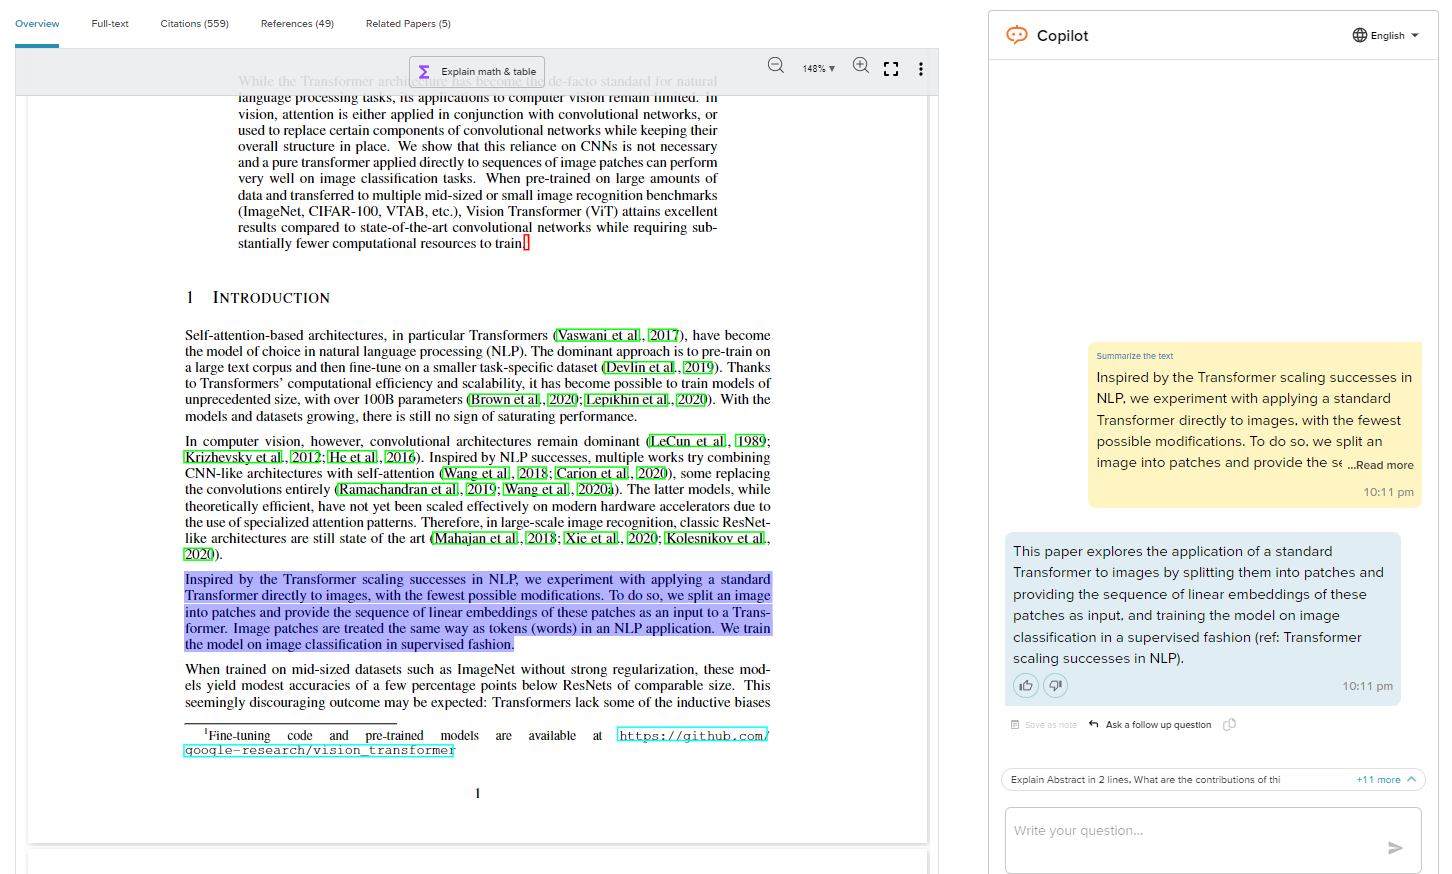
\includegraphics{img/typeset-example.png}
	\caption{Schermafbeelding van SciSpace}
\end{figure}

\section{GPT-3}
\textit{Generative Pretrained Transformer 3} of GPT-3 is een taalmodel ontworpen door OpenAI. Dit taalmodel gebruikt een tweestapsleerparadigma waarbij het eerst ongesuperviseerd wordt getraind met een taalmodelleringsdoel en daarna gesuperviseerd wordt gefinetuned. Over drie versies heen is het model aanzienlijk vergroot, van anderhalf miljard parameters bij GPT-2 naar 175 miljard parameters bij GPT-3. Het model is getraind op niet-gecategoriseerde data van het internet en gebruikt datasets waaronder Common Crawl, WebText2, Books1, Books2, and Wikipedia \autocite{Radford2019, Li2022}.

\begin{figure}[H]
	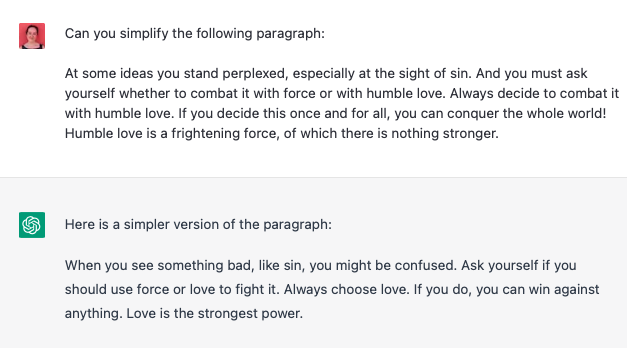
\includegraphics[width=10cm]{img/chatgpt-example-simplification-gooding.png}
	\caption{Afbeelding van Gooding 2022. De invoertekst is een paragraaf uit een niet-vermeld boek van de Russische schrijver Dostoevsky. Het resultaat van de meegegeven prompt is een transformatie dat iedere vorm van vooraf aangehaalde vereenvoudiging weergeeft. Lexicale, conceptuele en syntactische vereeenvoudiging worden op de invoertekst toegepast.}
\end{figure}

\begin{figure}[H]
	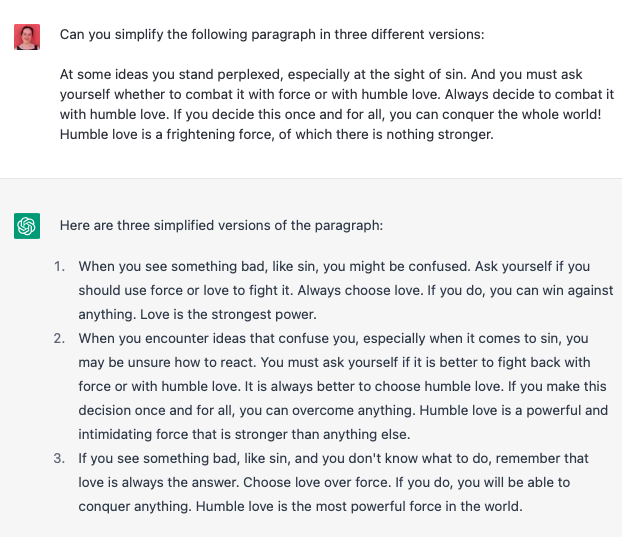
\includegraphics[width=10cm]{img/chatgpt-example-different-versions-gooding.png}
	\caption{Afbeelding van Gooding 2022. Gooding haalt verder aan dat modellen zoals ChatGPT op twee vlakken de leesbaarheid van een tekst kan bevorderen. Allereerst door het verlenen van verschillende mogelijke versies van een vereenvoudigingstaak.}
\end{figure}

\begin{figure}[H]
	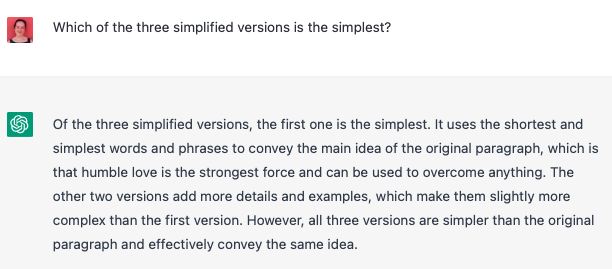
\includegraphics[width=10cm]{img/chatgpt-example-evaluation-gooding.png}
	\caption{Afbeelding van Gooding 2022.}
\end{figure}

\textcite{Lisowski2023} vergelijkt de twee OpenAI taalmodellen met een \textit{mixed-methods} onderzoek. Al blijken de twee heel gelijkaardig, het experiment benadrukt dat het ChatGPT-model gericht is op conversationele doeleinden met voorkeur als chatbot, terwijl GPT-3 een ML-model is bedoeld om met hoogstens één prompt te werken. De grootte van het GPT-3 model met 175 miljard parameters imposanter dan Chat-GPT. Daarnaast is de limiet bij het meest recente GPT-3 model is 4000 tokens. Verder haalt Lisowski aan dat de kwaliteit bij beide modellen sterk afhankelijk is van de invoer. De prompts moeten concreet genoeg zijn, om zo niet af te wijken van wat de gebruiker wilt \autocite{Lisowski2023}. Deze twee API's zijn nu vrij beschikbaar voor ontwikkelaars als betalende API \autocite{Brockman2023}.

\subsubsection{Beschikbare GPT-3 engines}

De documentatie van OpenAI\footnote{https://platform.openai.com/docs/} reikt vier verschillende engines voor het GPT-3 taalmodel aan, namelijk Davinci, Curie, Babbage en Ada. In Maart 2023 voegde een vijfde engine zich toe, namelijk GPT-3 Turbo wat de basis is achter Chat-GPT. Davinci-003 is het meest geavanceerde model dat alles kan wat de andere engines ook kunnen, met de meest menselijke antwoorden en geschikt voor taken zoals essays schrijven en code genereren. Curie is goed voor nuance maar minder menselijk dan Davinci, terwijl Ada en Babbage minder krachtig zijn en aangeraden worden voor eenvoudige taken zoals tekst aanvullen en sentiment analyse \autocite{Brockman2023}. 

\begin{figure}
	\begin{center}
		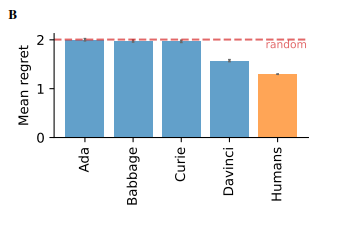
\includegraphics{img/chatgpt-engines-mean-regret.png}
		\caption{Afbeelding van \textcite{Binz2023}. Dit toont de \textit{mean regret} aan tussen de vier engines en de menselijke antwoorden.}
	\end{center}
\end{figure}

\subsubsection{Tools met GPT-3}

De mogelijkheden van OpenAI's ChatGPT en GPT-3 modellen zijn nog volop in ontwikkeling, maar er zijn al enkele vergelijkende onderzoeken uitgevoerd. Uit het experiment van \textcite{Goyal2022} blijkt dat \textit{zero-shot} samenvattingen met GPT-3 beter presteren dan \textit{fine-tuned} modellen. Daarnaast haalt \textcite{Mottesi2023} verschillende tools aan die gebruik maken van de GPT-3 API, waaronder Jasper AI en ChatSonic. Ook voor het onderwijs zijn er mogelijkheden, zoals de hoge toegankelijkheid en granulaire personalisatie van het GPT-3 model \autocite{Roose2023, Garg2022}. Echter, GPT-3 is niet geschikt voor alle taken, zoals sentimentanalyse en -classificatie, waarvoor een kleinschaliger taalmodel beter presteert \autocite{Li2022}. Bovendien is er aandacht voor de ecologische effecten van de grote omvang van deze modellen, waarvoor alternatieve oplossingen zoals het gebruik van Cloud-infrastructuur en geschikte model finetuning worden voorgesteld \autocite{Strubell2019, Simon2021}.

% Onderzoek naar OpenAI's ChatGPT en GPT-3 modellen bevindt zich in een vrij vroeg stadium, al zijn er wel enkele vergelijkende onderzoeken die de kracht en zwaktes van deze technologieën aantonen. Het experiment van \textcite{Goyal2022} achterhaalt het gebruik van \textit{zero-shot} samenvattingen buiten generieke samenvattingen. Het onderzoek staat stil bij de impact van prompt-gebaseerde modellen voor het automatisch samenvatten van nieuwsartikelen. Daarnaast maakte het onderzoek gebruik van text-davinci-002 als case study. Uit het experiment besluiten de onderzoekers dat \textit{zero-shot} samenvattingen met GPT-3 beter presteren dan \textit{fine-tuned} modellen, en dat bestaande automatische metrieken zoals BLEU, ROUGE en BERTScore niet geschikt zijn om \textit{zero-shot} samenvattingen te beoordelen. Verder blijkt dat zero-shot samenvattingen meer coherentie en relevantie hebben voor trefwoord-gebaseerde samenvattingen, terwijl aspect-gebaseerde samenvattingen nog vaak blijven te falen.

% \textcite{Mottesi2023} haalt lees- en schrijftools aan die gebruik maken van de GPT-3 API. Jasper AI is een chatbot bestemd voor customer support en een virtueel assistent voor e-commerce. ChatSonic is een tool gericht om social media posts of nieuwsartikelen te generere op basis van een kernzin of kernwoord. Verschillende artikels vermelden de mogelijkheden voor het gebruik van GPT-3 en ChatGPT in het onderwijs. \textcite{Roose2023} haalt zo de hoge toegankelijkheid, engagement bij scholieren en granulaire personalisatie aan dat het GPT-3 model toe in staat is. \textcite{Garg2022} ziet in GPT-3 en ChatGPT een portaalfunctie, om scholieren te helpen bij het opzoeken van nieuwe informatie tijdens de les en bij het instuderen.

% \textcite{Li2022} benadrukt dat GPT-3 voor simpele taken \textit{overkill} is. Taken buiten het genereren van teksten, zoals sentimentanalyse en -classificatie, worden beter met een kleinschaliger taalmodel, zoals BERT en verwante modellen, uitgevoerd. Deze keuze beïnvloedt het budget, want GPT-3 is een API waar per token wordt betaald, terwijl BERT gratis en open-source is. \textcite{Strubell2019, Simon2021} halen de ecologische effecten aan van ontwikkelaars die te snel voor deze modellen grijpen. Er is een bewezen effect kleinere modellen, gebruik van Cloud-infrastructuur en ten slotte een geschikte model finetuning bijdragen tot efficiëntere alsook minder klimaatbelastende effect.

\subsubsection{Vergelijking met andere taalmodellen}

De architectuur tussen GPT-3 en BERT is volgens \textcite{Mottesi2023} het meest opvallende verschil. GPT-3 is een autoregressief model en houdt daarmee enkel rekening met de linkercontext bij het voorspellen of genereren van tekst. BERT daarentegen is bidirectioneel en neemt zowel de linker- als de rechtercontext in overweging. De bidirectionele werking is geschikt voor sentimentanalyse waarbij begrip van de volledige zincontext noodzakelijk is. GPT-3 heeft toegang tot meer informatie (45TB) dan BERT (3TB), wat het een voordeel kan geven bij het samenvatten of het vertalen. Ten slotte zijn er ook verschillen in grootte. Hoewel beide modellen erg groot zijn, GPT-3 is aanzienlijk groter dan de voorganger vanwege de uitgebreide trainingsdatasetgrootte \autocite{Brown2020}.

LLaMa of Large Language Model Meta AI is een generatief taalmodel met potentieel dat sterker is dan GPT-3 en soortgelijke modellen, terwijl het van tien keer minder parameters gebruik maakt, maar is nog niet beschikbaar als online webtoepassing of API \autocite{Hern2023, Touvron2023}.


\begin{figure}[H]
	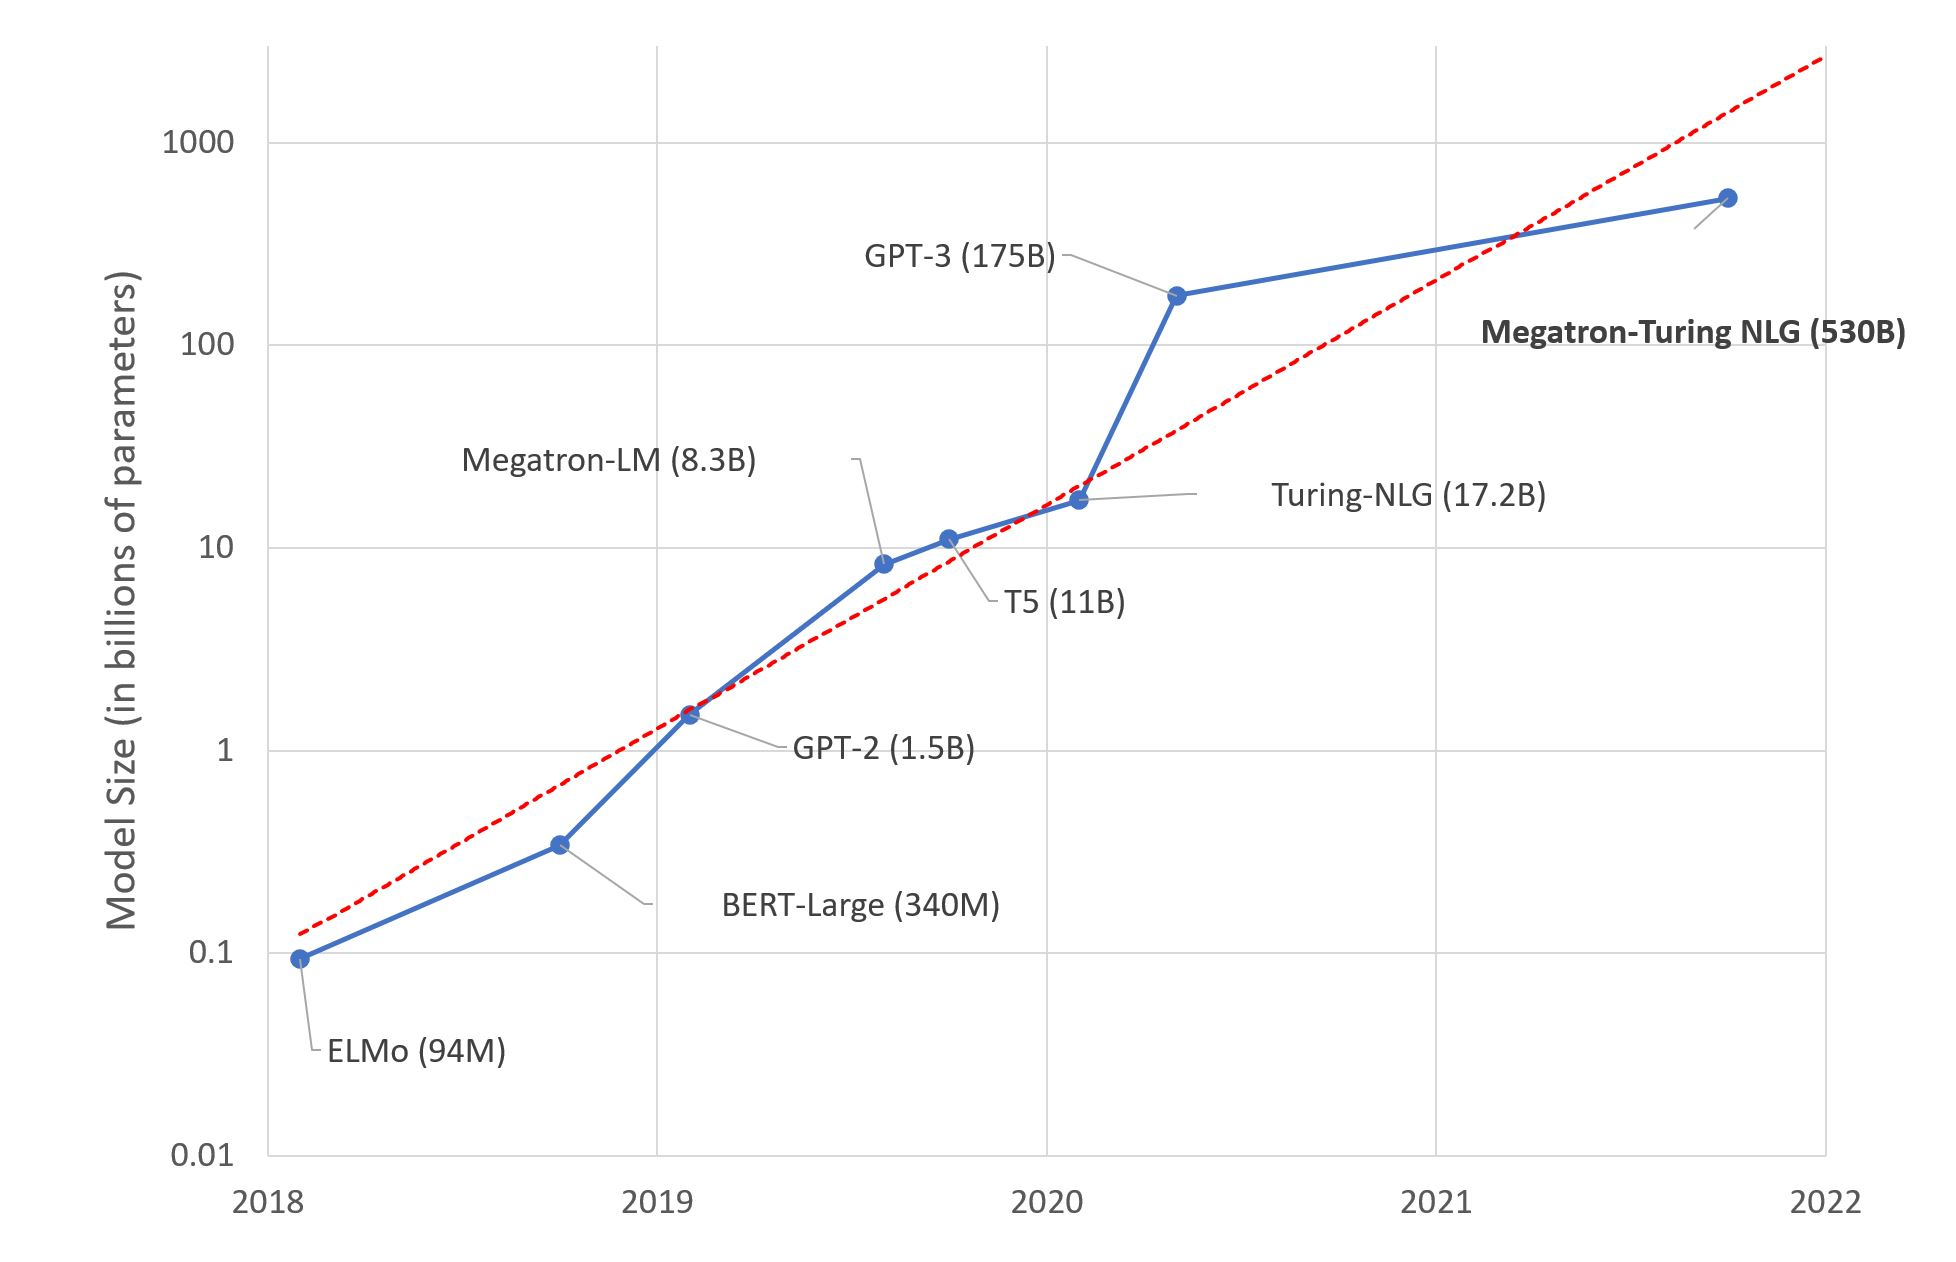
\includegraphics{img/graph-language-models.png}
	\caption{Afbeelding van \textcite{Simon2021}. De evolutie van pre-trained taalmodellen wordt hier weergegeven tot eind 2022. De performantie van de modellen ten opzichte van de grootte volgt een lineaire functie.}
\end{figure}

\subsubsection{GPT-3 finetuning}

\begin{tabular}{|c|p{7cm}|p{5cm}|}
	\hline
	Parameter & Omschrijving & Mogelijke waarden \\
	\hline
	model & Het GPT-3 model om te gebruiken & davinci, curie, babbage, ada, text-davinci-002, text-curie-001, text-babbage-001, text-ada-001, davinci-codex \\
	\hline
	temperature & De gulzigheid van een generatief model. Een lagere waarde zal conservatieve en voorspelbare tekst teruggeven. Hogere waarden zullen meer gevarieerde en onverwachtse tekst teruggeven, wat beter werkt bij creatieve toepassingen. & Een kommagetal tussen 0 en 1. \\
	\hline
	max\_tokens & Het maximaal aantal tokens (woorden of subwoorden) dat het generatief model kan teruggeven. & Een getal tussen 1 and 2048. \\
	\hline
	top\_p & Vergelijkbaar met temperature, maar deze waarde onderhoudt de probability distribution voor common tokens. Hoe lager de waarde, hoe waarschijnlijker de woordenschat dat het model zal overwegen bij het genereren van tekst. Een hoge waarde is toepasselijker wanneer een toepassing gericht is op nauwkeurigheid en correctheid. & Een kommagetal tussen 0 en 1. \\
	\hline
	stop & Een tekstwaarde (woord/symbool) tot waar het model zal genereren. When the model generates a string that matches any of the specified strings, it stops generating text. & Een lijst van string-waarden, of een enkele string. \\
	\hline
	presence\_penalty & Factor die bepaalt hoe regelmatig woorden voorkomen. & Een kommagetal tussen 0 en 1 \\
	\hline
\end{tabular}

\subsection{Bing AI}

Microsoft en OpenAI werken nauw samen. Zo maakt het conversationele taalmodel van Bing ook gebruik van GPT-3. Deze chatbot bouwt verder en biedt zo verwijzingen en referenties aan naar andere websites. Deze verwijzingen zijn volgens mogelijk door de Prometheus-technologie van Microsoft \autocite{Ribas2023}.

Prometheus is een eigen technologie die door Bing is ontwikkeld. Het AI-model is volgens \textcite{Ribas2023} de eerste van zijn soort die de Bing-index-, ranking- en antwoordresultaten combineert met het redeneervermogen van OpenAI’s GPT-modellen. Prometheus maakt gebruik van de kracht van Bing en GPT om iteratief via een component genaamd \textit{Bing Orchestrator} een set interne queries te genereren met als doel binnen gegeven gesprekscontext een nauwkeurig antwoord op gebruikersqueries te bieden \autocite{Ribas2023}.

\begin{figure}[H]
	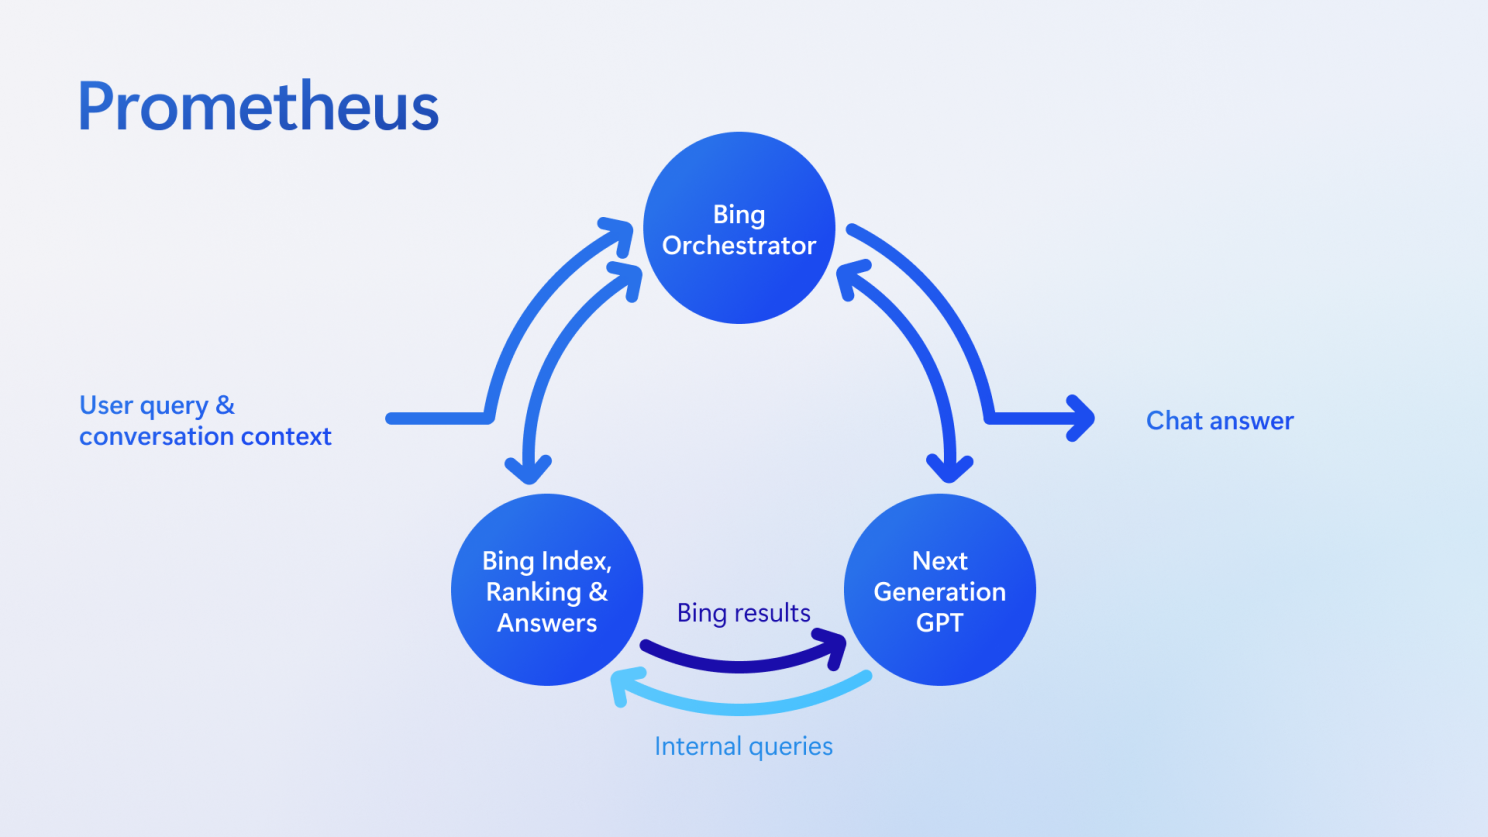
\includegraphics[width=6cm]{img/bing-ai-prometheus.png}
	\caption{Afbeelding van \textcite{Ribas2023}.}
\end{figure}

Bing AI is nu in testfase met wachtlijst en bestaat in de vorm van een webpagina en een browserextensie voor Microsoft Edge. Onderzoek naar deze chatbot staat nog in de kinderschoenen en er is nood aan onderzoek naar de credibiliteit en correctheid van de verwijzingen. Deze chatbot gebruikt een combinatie van extraherende en abstraherende samenvattingen. In tegenstelling tot GPT-3 is er geen officiële API beschikbaar. Daarnaast is de limiet ook lager met 2000 tokens per bericht tijdens een conversatie. 

\begin{figure}[H]
	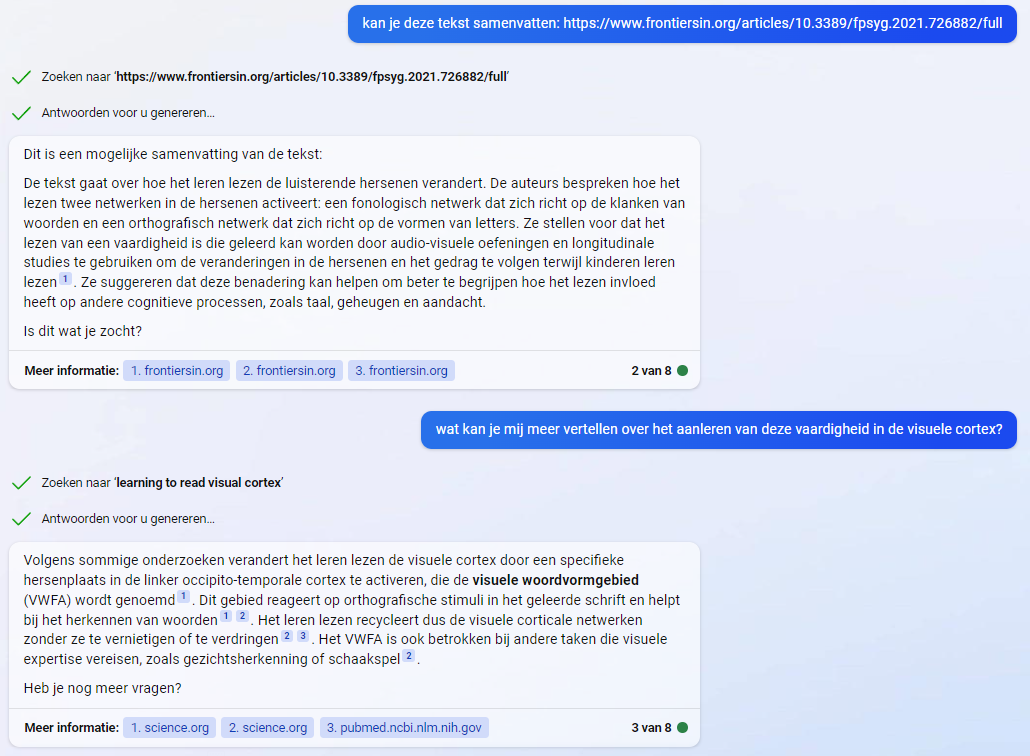
\includegraphics{img/bing-ai-chatbot-example.png}
	\caption{In deze afbeelding wordt er een online wetenschappelijk artikel meegegeven. Er wordt geen titel of onderwerp meegegeven, maar de Bing AI chatbot is in staat om een abstraherende samenvatting te maken van het artikel. Daarna geeft de chatbot verder uitleg over een bepaald onderwerp en geeft het extra referenties mee.}
\end{figure}

Het bedrijf DuckDuckGo dat instaat voor de gelijknamige zoekmachine probeert een gelijkaardig initiatief. Met \textit{DuckAssist} biedt de onderneming een eigen AI-oplossing aan om een algemene doelgroep te ondersteunen bij het opzoeken van (nieuwe) informatie. Zij halen informatie direct uit enkel Wikipedia pagina's \autocite{Weinberg2023}. Daarnaast maakt dit DuckAssist ook gebruik van het GPT-3 model. Nadelig heeft deze toepassing voorlopig beschikking tot een kleinere zoekruimte dan Bing AI, wat gebruik maakt van meer sites inclusief onderzoekssites zoals ResearchGate \autocite{Mcauliffe2023}. Deze beperkte zoekruimte reduceert de kans op incorrecte of foutieve informatie volgens \textcite{Weinberg2023}, al is dit eerder een intuïtie van het bedrijf.


\subsection{Huggingface en taalmodellen via API}

In recente literatuur is Huggingface beschreven als een platform of portaalsite voor het delen van ML-modellen en datasets. De bibliotheek biedt een scala aan API's en tools die gemakkelijk te downloaden en trainen zijn voor pretrained modellen voor prevalente NLP-taken, zoals tekstclassificatie, taalmodellering en samenvatting. Deze modellen kunnen worden gefinetuned op specifieke datasets, waardoor ontwikkelaars snel modellen kunnen bouwen en inzetten voor vereenvoudigings- en samenvattingstaken. Voor wetenschappelijke documenten en artikelen bestaan er enkel modellen en datasets: \footnote{https://huggingface.co/sambydlo/bart-large-scientific-lay-summarisation}, \footnote{https://huggingface.co/haining/scientific\_abstract\	_simplification}

\subsection{Conclusie}

Experten halen het GPT-3 model en ChatGPT aan als de toekomst voor gepersonaliseerde en adaptieve uitleg aan scholieren. Bing AI biedt een extra dat revolutionair kan zijn bij het opzoeken van uitleg voor zoektermen, zonder het verlies aan bronvermelding. Huidige toepassingen staan mogelijks in een spreekwoordelijke schaduw eenmaal leessoftware voor scholieren met dyslexie worden ontwikkeld met AI. De mogelijkheden van GPT-3 zijn eindeloos en toepassingen die hiervan gebruik maken, kunnen in het onderwijs ingezet worden als ondersteunende software.

\section{Conclusie}

De noden van scholieren met fonologische dyslexie in de derde graad van het middelbaar gaan verder dan gewoon moeizaam lezen.  Het ontcijferen en automatiseren van woordeherkenning gebeurt langzaam. Er zijn bewezen voordelen van manuele tekstvereenvoudiging en adaptieve visuele weergaven op kinderen en jongeren met dyslexie. De leesbaarheid van wetenschappelijke artikelen bevindt zich in een neergaande trend. Het formaat, gebruik van vakjargon en ingewikkelde woordenschat en ten slotte de moeizame syntax en zinsbouw sluiten een algemene doelgroep uit bij het lezen van wetenschappelijke artikelen. Enkel wetenschappelijk geletterden zijn in staat om deze artikelen te lezen. Het uniforme formaat van een wetenschappelijk artikel biedt kansen aan voor een geautomatiseerde aanpak tot het vereenvoudigen van een tekst.

Experten halen meerdere bewezen tactieken aan om teksten automatisch te vereenvoudigen op maat voor een scholier met dyslexie. Handmatig worden teksten vereenvoudigd aan de hand van leesbaarheidsformules of intuïtie. Zinnen moeten lexicaal, syntactisch en semantisch worden vereenvoudigd. Teksten samenvatten maakt de tekst korter zonder het verlies van de kernboodschap. Voor deze vier transformaties zijn er taalmodellen beschikbaar in de vorm van API's of open-source software. Huidige software dat de overheid uitleent aan scholieren met dyslexie in het middelbaar onderwijs fungeert voornamelijk als voorleessoftware. Nieuwe en opkomende technologieën en taalmodellen zoals GPT-3 blinken uit om tekstvereenvoudiging mogelijk te maken. De ontwikkeling met LLM's is in opmars, maar ontwikkelaars moeten bewust zijn dat andere taalmodellen zoals BERT voor taken zoals semantische analyse minder rekenkracht vereisen voor eenzelfde en soms beter resultaat. 
%%=============================================================================
%% Methodologie
%%=============================================================================

\chapter{\IfLanguageName{dutch}{Methodologie}{Methodology}}%
\label{ch:methodologie}

% Door de vergaarde kennis uit de literatuurstudie in hoofdstuk \ref{ch:stand-van-zaken} over de mogelijke noden van scholieren met dyslexie, de complexiteit van wetenschappelijke artikelen, de technieken voor MTS en ATS, en de bijhorende valkuilen bij taalverwerking met AI, kunnen onderzoeksmethoden worden toegepast om een antwoord te vinden op de onderzoeksvraag. 

Om een antwoord te vormen op de onderzoeksvraag, moet de vergaarde kennis uit de literatuurstudie in drie onderzoeksmethoden. Eerst staat het onderzoek stil bij de vereiste functionaliteiten om gepersonaliseerde ATS te kunnen realiseren. Vervolgens achterhaalt het onderzoek het geschikte taalmodel voor gepersonaliseerde ATS. Tenslotte volgt de ontwikkeling van een prototype voor ATS-vereenvoudiging van wetenschappelijke artikelen. Zo doelt dit onderzoek om de haalbaarheid voor een toepassing voor gepersonaliseerde ATS te achterhalen aan de hand van een prototype. Dit prototype moet in staat zijn om wetenschappelijke artikelen te vereenvoudigen op maat voor scholieren met dyslexie in de derde graad van het middelbaar onderwijs.

\section{Requirementsanalyse}
\label{sec:requirementsanalyse}

Om het ontwikkelingsproces van het prototype gericht te sturen, moet het onderzoek MTS- en ATS-technologieën in bestaande tools nagaan. Zo gebeurt het verkennen en experimenteren op ATS-technieken bij beschikbare tools door een kwalitatief onderzoek in de vorm van een requirementsanalyse. Het resultaat van deze onderzoeksfase is een moscow-schema dat de benodigde functionaliteiten voor een toepassing met ATS definieert, met als doel een vergelijkbare toepassing aan te bieden voor gepersonaliseerde ATS van wetenschappelijke artikelen met de kwaliteiten van gepersonaliseerde MTS. Daarnaast achterhaalt de onderzoeksfase de ontbrekende MTS-functionaliteiten die tabel \ref{table:benefits-mts} in de literatuurstudie uitwees. De geteste toepassingen, opgesomd in tabel \ref{table:shortlist-tools}, beschikken over (gepersonaliseerde) ATS-technieken. Deze lijst omvat erkende toepassingen van de overheid en toepassingen die leerkrachten of scholieren kunnen gebruiken om teksten te vereenvoudigen. Met deze onderzoeksmethode kan het onderzoek een antwoord geven op de volgende twee deelvragen van het onderzoek.

\begin{itemize}
	\item Welke functies ontbreken AI-toepassingen om geautomatiseerde tekstvereenvoudiging mogelijk te maken voor scholieren met dyslexie in de derde graad middelbaar onderwijs?
	\item Welke manuele methoden voor tekstvereenvoudiging komen niet in deze tools voor?
\end{itemize}

Figuur \ref{img:flowchart-requirementsanalyse} toont de flowchart om de requirementsanalyse te kunnen uitwerken.

\begin{figure}[H]
	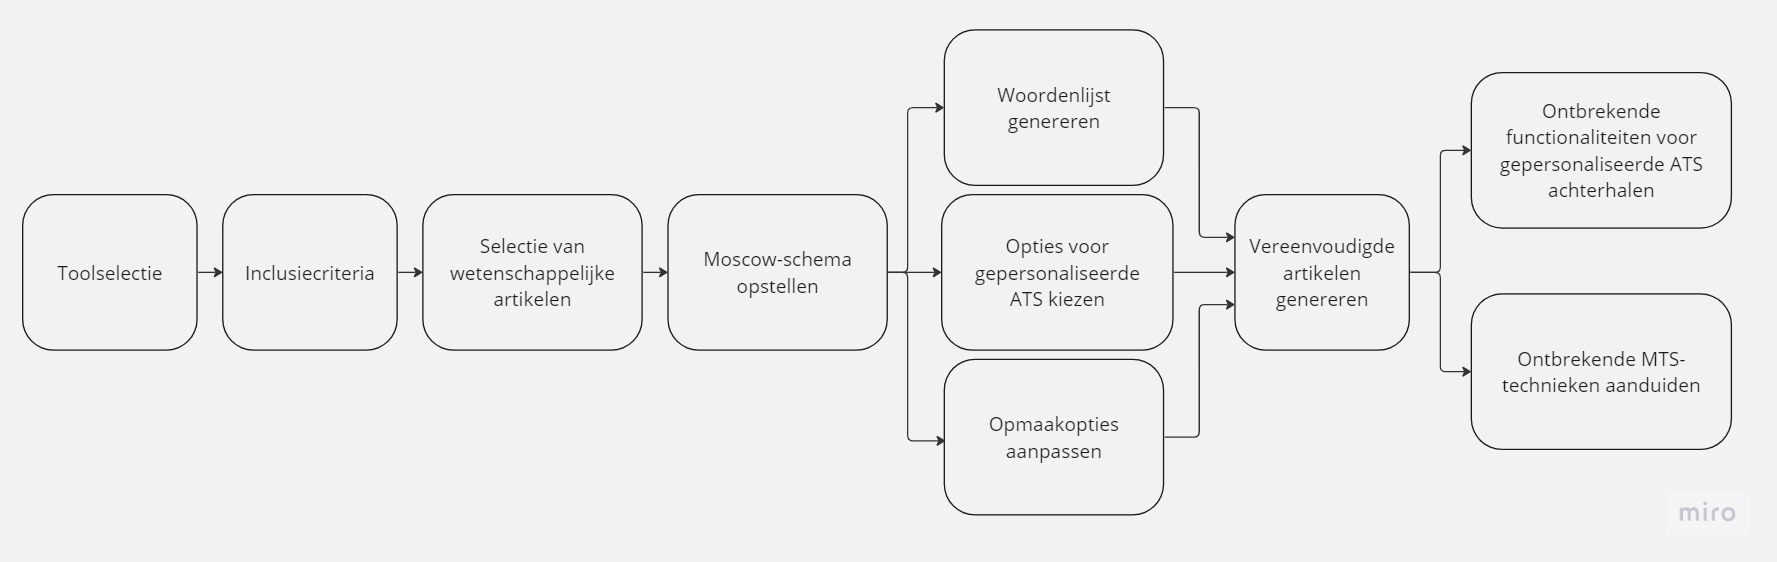
\includegraphics[width=\linewidth]{img/flowchart-requirementsanalyse.jpg}
	\caption{Het benodigde stappenplan bij de requirementanalyse.}
	\label{img:flowchart-requirementsanalyse}
\end{figure}

% TOOLSELECTIE 
Allereerst start het onderzoek met een toolselectie. Zoals aangewezen in sectie \ref{sec:beschikbare-tools-en-taalmodellen}, leent de overheid vijf softwarepakketten uit aan middelbare scholen. Echter neemt de requirementsanalyse drie van deze vijf in de analyse op, want hun functionaliteiten zijn passend voor deze doelgroep. De overige twee zijn minder aanwezig in het onderwijs. Daarnaast toont een zoekopdracht aan dat deze tools geen LS toepassen. 

Naast deze erkende softwarepakketten kunnen online beschikbare tools ook scholieren met dyslexie ondersteunen bij het begrijpend lezen van wetenschappelijke artikelen met ATS, zoals bewezen in \textcite{Bingel2018}. Daarom betrekt de requirementsanalyse enkel tools met onderschreven ATS-functionaliteiten en laat daarmee pure samenvattingstools erbuiten. Tabel \ref{table:shortlist-tools} toont een overzicht van de te experimenteren tools.

\begin{center}
	\begin{table}[H]
		\begin{tabular}{ | m{6cm} | m{6cm} | } 
			\hline
			\textbf{Erkende software} & \textbf{Online beschikbare tools} \\
			\hline
			Sprintplus (E1) & Simplish (O1) \\
			Kurzweil3000 (E2) & SciSpace (O2) \\ 
			AlineaSuite (E3) & Rewordify (O3) \\
			& ChatGPT (O4) \\
			& Bing Chat (O5) \\
			\hline
		\end{tabular}
		\caption{Shortlist van uit te testen tools en toepassingen voor tekstvereenvoudiging.}
		\label{table:shortlist-tools}	
	\end{table}
\end{center}

% Inclusiecritera
Vervolgens bouwt het onderzoek een lijst op van de toetsingscriteria. Zo dienen de MTS-technieken uit tabel \ref{table:scientific-paper-struggles} en tabel \ref{table:manual-simplification} als bouwstenen voor het opstellen van de toetsingscriteria. Tabel \ref{table:criteria-requirementsanalysis} geeft een opsomming van de MTS-technieken waaraan tools moeten voldoen. Daarnaast dient dit schema om een inschatting van de functionaliteiten van deze tools te maken.

\begin{center}
	\begin{table}[H]
		\begin{tabular}{ | m{4cm} | m{11cm} | } 
			\hline
			\textbf{MTS-techniek} & \textbf{Functionaliteit} \\
			\hline
			Lexicale & Gepersonaliseerde LS, ofwel woordenschat dat niet te hooggegrepen is. Gekende woordenschat mag blijven. \\
			vereenvoudiging & Woorden met minder lettergrepen gebruiken \\
			& Extra uitleg schrijven bij zinnen \\
			& Paragrafen herschrijven zodat ze eerst uitleg geven op een high-level niveau, vervolgens lagen van complexiteit toevoegen om de lezer te begeleiden \\
			& Woordenlijst aanmaken \\
			& Idiomen vervangen door eenvoudigere synoniemen \\
			\hline
			Syntactische & Zinnen inkorten \\
			vereenvoudiging & Verwijswoorden aanpassen \\
			& Voorzetseluitdrukkingen aanpassen \\
			& Samengestelde werkwoorden aanpassen \\
			& Actieve stem toepassen \\
			& Enkel regelmatige werkwoorden gebruiken \\
			\hline
			Structurele & Achtergrondkleur aanpassen \\
			aanpassingen & Woord- en karakterspatiëring \\
			& Consistente lay-out \\
			& Duidelijk zichtbare koppenstructuur \\
			& Huidige positie benadrukken \\
			& Waarschuwingen geven omtrent formulieren en sessies \\
			& Inhoud visueel groeperen \\
			& Tekst herschrijven als tabel \\
			& Tekst herschrijven als opsomming \\
			\hline
		\end{tabular}
		\caption{Richtlijnen waarop het onderzoek de toepassingen aftoetst in de requirementsanalyse.}
		\label{table:criteria-requirementsanalysis}	
	\end{table}
\end{center}

Als realistisch testmateriaal, maken de experimenten gebruik van twee gepubliceerde wetenschappelijke artikelen. Zo kunnen deze artikelen relevant zijn voor leerkrachten om aan scholieren in de derde graad van het middelbaar onderwijs te geven als leesvoer. Beide artikelen volgen de kenmerken van een wetenschappelijk artikel, zoals beschreven in tabel \ref{table:scientific-paper-struggles}. Daarnaast gebruiken ze vakjargon en wetenschappelijke concepten in een compact formaat. Tabel \ref{table:referentieteksten-bronvermelding} geeft een overzicht van de twee artikelen en een bijhorende bronvermelding.

\begin{center}
	\begin{table}[H]
		\begin{tabular}{ | m{10cm} | m{5cm} | } 
			\hline
			\textbf{Titel} & \textbf{Bronvermelding} \\
			\hline
			De controle op het gebruik van algoritmische surveillance- onder druk? Een exploratie door de lens van de relationele ethiek & \autocite{VanBrakel2022} \\
			\hline
			Nederland versus België: verschillen in economische dynamiek en beleid. & \autocite{Sleuwaegen2022} \\
			\hline
		\end{tabular}
		\caption{Bronvermeldingen voor de twee wetenschappelijke artikelen.}
		\label{table:referentieteksten-bronvermelding}
	\end{table}
\end{center}

% 4. 
Om een overzicht te hebben van de functionaliteiten volgens prioriteit, bouwt het onderzoek een moscow-schema vanuit de opgestelde richtlijnen. Zo komen belangrijke functionaliteiten, die nodig zijn om gepersonaliseerde tekstvereenvoudiging met ATS mogelijk te maken, in de categorie \textit{must-haves} terecht. Alle vereiste functionaliteiten om (gepersonaliseerde) ATS mogelijk te maken, moet als \textit{must-have} in het moscow-schema voorkomen. Irrelevante functionaliteiten binnen de scope van een prototype of niet toepasselijk voor de doelgroep plaatst het onderzoek als \textit{wont-have}.

\begin{center}
	\begin{table}[H]
		\begin{tabular}{ | m{4cm} | m{11cm} | } 
			\hline
			\textbf{MoSCoW-principe} & \textbf{Functionaliteit} \\
			\hline
			Must-have & Gepersonaliseerde LS, ofwel woordenschat dat niet te hooggegrepen is. Gekende woordenschat mag blijven. \\
			& Woorden met minder lettergrepen gebruiken. \\
			& Woordenlijst aanmaken na handmatige CWI. \\
			& Wetenschappelijke artikelen in PDF-vorm opladen. \\
			& Structurele aanpassingen toepassen op de oorspronkelijke tekst. \\
			& Personaliseerbare opmaakopties, waaronder lettertype -en grootte aanpassen, tekstformaat aanpassen, achtergrondkleur aanpassen. \\
			& Duidelijk zichtbare koppenstructuur. \\
			& Tekst herschrijven als opsomming. \\
			\hline
			Should-have & \\
			& Tekstanalyse \\
			& Extra (in-line) uitleg schrijven bij moeilijke woordenschat. \\
			& Personaliseerbare PDF- of Word-document lay-out. \\
			& Uitvoer als PDF of Word-bestand teruggeven. \\
			& Wetenschappelijke artikelen in PDF-vorm opladen met OCR. \\
			& Tekstanalyse voor en na de vereenvoudiging aanbieden. \\
			\hline
			Could-have 
			& Gebruikersfeedback \\
			& Woordenschat genereren na automatische CWI. \\
			& Huidige positie benadrukken. \\
			& Waarschuwingen geven omtrent formulieren en sessies. \\
			& Enkel regelmatige werkwoorden gebruiken. \\
			& Extraherende samenvatting \\
			& Abstraherende samenvatting \\
			& Tekst herschrijven in tabelvorm \\
			\hline
			Wont-have & \\
			& Mobiele versie of \textit{responsive design}. \\
			& Audio-uitvoer \\
			& Integratie met externe toepassingen, waaronder spelcheckers. \\
			\hline
		\end{tabular}
		\caption{Het moscow-schema voor de requirementsanalyse.}
		\label{img:moscow-table}
	\end{table}
\end{center}

\medspace

Vervolgens komen experimenten rond de opties rond gepersonaliseerde ATS aan bod. Eindgebruikers moeten wetenschappelijke artikelen kunnen opladen. Eindgebruikers kunnen enkel pdf's inladen bij SprintPlus, Kurzweil3000, AlineaSuite, Simplish, Rewordify en SciSpace. In tegenstelling tot Bing Chat en ChatGPT waarbij \textit{plain-text} of een link naar het wetenschappelijk artikel de enige vormen van invoer zijn. De tekstinhoud uit de PDF extraheren gebeurt dan manueel en deze tekst dient daarna als invoer voor de chatbot. Beide chatbots krijgen de prompt, gevolgd door een stuk van het wetenschappelijk artikel. Met zes verschillende prompts kan het onderzoek de functionaliteit om LS, SS of structurele aanpassingen op een tekst door een toepassing achterhalen. Tabel \ref{table:tested-prompts-requirementsanalysis} vermeldt de toegepaste prompts. Toepassingen krijgen eerst een link van het wetenschappelijk artikel. Als de toepassing hier niet over beschikt, dan krijgt de chatbot de tekstinhoud van het wetenschappelijk artikel in \textit{plain-text} mee. 

\begin{center}
	\begin{table}[H]
		\begin{tabular}{ | m{2cm} | m{14cm} | } 
			\hline
			\textbf{Naam} & \textbf{Prompt} \\
			\hline
			P1 & Vereenvoudig deze tekst. \\
			\hline
			P2 & Vereenvoudig deze tekst voor studenten (16-18 jaar) door moeilijke woorden te vervangen, vakjargon te schrappen, woorden langer dan 18 letters te vervangen, acroniemen voluit te schrijven, een woord slechts eenmaal door een synoniem te vervangen, korte uitleg te geven wanneer dat nodig is, en percentages te vervangen. \\
			\hline
			P3 & Vereenvoudig een tekst door deze op te delen in kortere zinnen van maximaal tien woorden. Verander voornaamwoorden als 'zij', 'hun' of 'hij' in namen. Vervang complexe zinsconstructies en voorzetselzinnen door eenvoudiger alternatieven, maar laat ze ongewijzigd als er geen eenvoudiger optie beschikbaar is. \\
			\hline
			P4 & Schrijf de tekst als opsomming. \\
			\hline
			P5 & Schrijf de tekst in tabelformaat. \\
			\hline
			P6 & Genereer op basis van deze tekst een woorden- en synoniemenlijst. \\
			\hline
		\end{tabular}
		\caption{De toegepaste GPT-3-prompts in de requirementsanalyse.}
		\label{table:tested-prompts-requirementsanalysis}
	\end{table}
\end{center}

\medspace

Daarna voert het onderzoek experimenten rond gepersonaliseerde opmaakopties uit. Kurzweil, SprintPlus en AlineaSuite bieden opmaakopties aan in het instellingenscherm. Zo kunnen eindgebruikers het lettertype, -kleur -en grootte en de achtergrondkleur aanpassen naar keuze. Als een toepassing niet over opmaakopties beschikt, dan stopt het experiment rond opmaakopties voor die toepassing.

\medspace

Tot slot test het onderzoek de capaciteiten om het formaat van teksten aan te passen aan de hand van structurele aanpassingen. Zo vragen P4 en P5 specifiek naar een structurele aanpassing, terwijl P1, P2 en P3 minstens een doorlopende tekst als resultaat verwachten. Andere beschikbare tools missen checkboxen of keuzelijsten om deze keuze aan te reiken, waardoor het testen van deze functionaliteit niet mogelijk is.

\section{Vergelijkende studie}
\label{sec:vergelijkende-studie}

Om wetenschappelijke artikelen met gepersonaliseerde ATS te vereenvoudigen, moet dergelijk toepassing gebruikmaken van een geschikt taalmodel. Zo moet de uitvoer van het prototype een vereenvoudigde versie van een wetenschappelijk artikel kunnen geven, specifiek voor de noden van scholieren met dyslexie in de derde graad van het middelbaar onderwijs. Om de uitvoer van het prototype nauwkeurig af te stemmen, vereist het onderzoek een antwoord op de volgende vraag.

\begin{itemize}
	\item Welk taalmodel is geschikt voor tekstvereenvoudiging met ATS van wetenschappelijke artikelen voor scholieren met dyslexie in de derde graad van het middelbaar onderwijs, met dezelfde of gelijkaardige kwaliteiten als gepersonaliseerde tekstvereenvoudiging met MTS?
\end{itemize}

Er zijn weinig gespecialiseerde taalmodellen beschikbaar om wetenschappelijke artikelen te vereenvoudigen. Daarom beoordeelt de vergelijkende studie alle vermelde taalmodellen opgesomd in tabel \ref{table:vergelijkende-studie-taalmodellen}.

\begin{center}
	\begin{table}[H]
		\begin{tabular}{ | m{4cm} | m{11cm} | } 
			\hline
			\textbf{Verwijzing} & \textbf{Taalmodel} \\
			\hline
			T1 & Haining Scientific Abstract Simplification \\
			\hline
			T2 & BART-based Scientific Lay Summarizer \\
			\hline
			T3 & Keep It Simple\\
			\hline
			T4 & GPT-3 \\
			\hline
		\end{tabular}
		\caption{Gebruikte taalmodellen in de vergelijkende studie}
		\label{table:vergelijkende-studie-taalmodellen}
	\end{table}
\end{center}

De vergelijkende studie bestaat uit vijf fasen, weergegeven op de \textit{flowchart} in figuur \ref{img:flowchart-vergelijkende-studie-metrics}. Zo vergelijkt deze onderzoeksfase de leesgraadscores van de oorspronkelijke wetenschappelijke artikelen zoals in sectie \ref{sec:requirementsanalyse}, met referentieteksten vereenvoudigd met MTS en teksten vereenvoudigd met ATS. Met een \textit{mixed-methods} onderzoek kan de vergelijkende studie taalmodellen beoordelen op objectief en subjectief niveau. 

De gebruikte wetenschappelijke artikelen zijn identiek aan de taalmodellen in tabel \ref{table:referentieteksten-bronvermelding}. Om realistisch referentiemateriaal te verkrijgen, schrijven twee leerkrachten en twee leerlingen zonder dyslexie zelf een vereenvoudiging van de twee wetenschappelijke artikelen met MTS. Deze vier personen baseren zich op vooraf meegekregen richtlijnen, toegelicht in de bijlage \ref{ch:referentietekst}. 

\begin{figure}
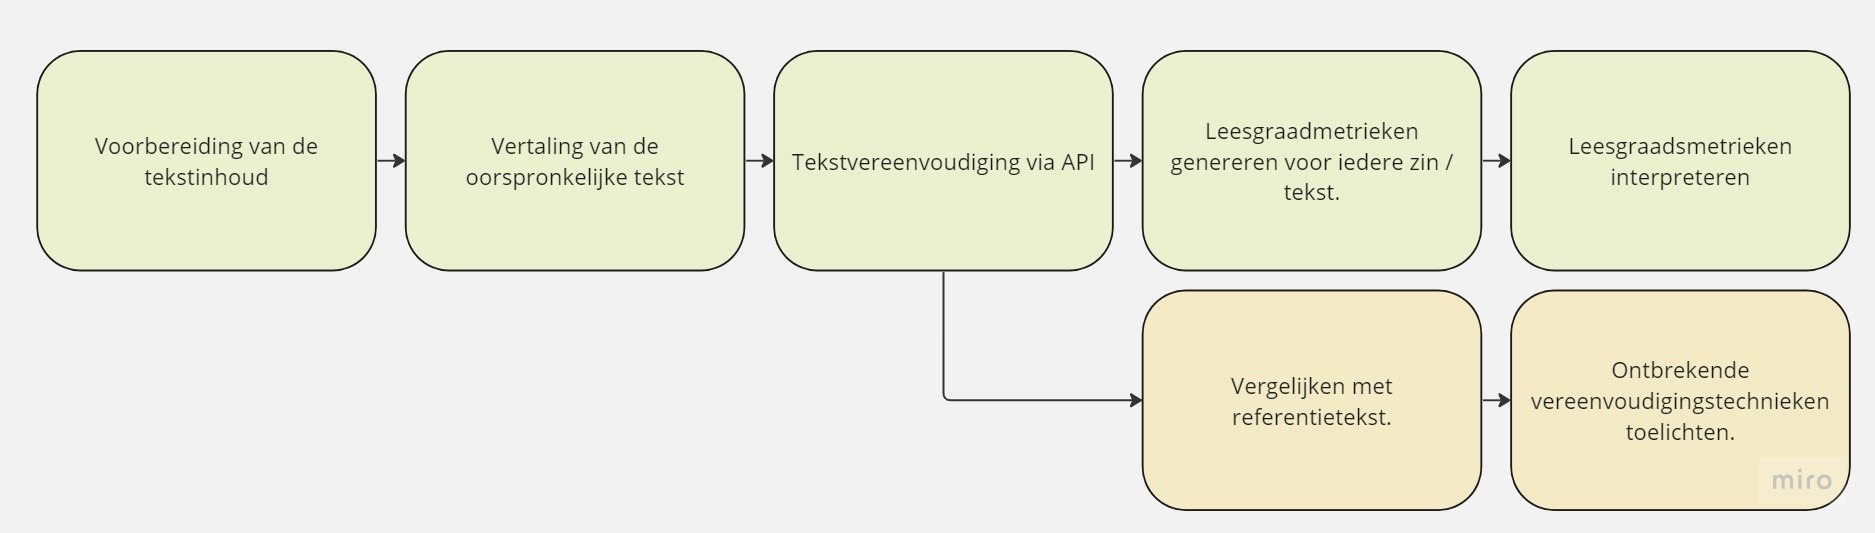
\includegraphics[width=\linewidth]{img/flowchart-vergelijkende-studie.jpg}
\caption{Het gevolgde stappenplan voor de vergelijkende studie.}
\label{img:flowchart-vergelijkende-studie-metrics}
\end{figure}

\medspace

% SCRIPT 1
Eerst volgt er een voorbereiding van de tekstinhoud. Allereerst haalt het script de inhoud van de map met wetenschappelijke artikelen op om deze vervolgens in een tekstbestand te plaatsen, zoals weergegeven in codeblok \ref{code:verg-studie-phase-1}. 

\begin{lstlisting}[language=Python, caption={Script voor fase 1 van de vergelijkende studie.}, label={code:verg-studie-phase-1}]
	def add_newline_after_dot(input_file, output_file):
	with open(input_file, 'r', encoding='utf-8') as file:
	text = file.read()
	text = re.sub(r'\d', '', text)
	modified_text = text.replace('.', '.\n')
	with open(output_file, 'w', encoding='utf-8') as file:
	file.write(modified_text)
	
	folder_path = 'scripts\pdf'
	original_scientific_papers = [f for f in os.listdir(folder_path)]
	
	for paper in original_scientific_papers:
	input_file =  folder_path + '/' + paper
	output_file = folder_path + '/' + 'RE_' + paper
	add_newline_after_dot(input_file, output_file)
\end{lstlisting} 

Vervolgens vertaalt het script de zinnen naar Engels. Het script, verwezen in script \ref{code:verg-studie-phase-2}, doorloopt alle tekstbestanden en vertaalt de tekstinhoud met de \textit{deep\_translator} python-bibliotheek. Zo bekomt het script een csv-bestand met twee kolommen: alle Nederlandstalige en alle vertaalde Engelstalige zinnen van één wetenschappelijk artikel. Als separator gebruikt het csv-bestand een \textit{pipe}-symbool.

\begin{center}
	\begin{lstlisting}[language=Python, caption={Script voor de tweede fase van de vergelijkende studie.}, label={code:verg-studie-phase-2}]
		output_csv = 'results.csv'
		
		def translate_dutch_to_english(dutch_text_file):
		with open(dutch_text_file, 'r', encoding='utf-8') as file:
		dutch_sentences = file.readlines()
		dutch_sentences = [sentence.strip() for sentence in dutch_sentences]
		
		english_sentences = []
		for sentence in dutch_sentences:
		translated = GoogleTranslator(source='nl', target='en').translate(sentence)
		english_sentences.append(translated)
		df = pd.DataFrame({'Dutch': dutch_sentences, 'English': english_sentences})
		df.to_csv(str(dutch_text_file).split('.')[0] + '.csv', index=False)
		
		
		folder_path = 'scripts/pdf/'
		original_scientific_papers = [f for f in os.listdir(folder_path)]
		
		for paper in original_scientific_papers:
		if paper.startswith('RE_') and paper.endswith('.txt'):
		print(f'STARTING {paper}')
		dutch_text_file = folder_path + paper
		translate_dutch_to_english(dutch_text_file)
	\end{lstlisting}
\end{center}


Na de vertaling van de tekstinhoud, stuurt het script API-calls voor iedere zin naar ieder taalmodel. Dit procesde taalmodellen aan om de inhoud van de wetenschappelijke artikelen te vereenvoudigen, weergegeven in listing \ref{code:verg-studie-phase-3}. Allereerst vindt een tokenisatiefase plaats. Daarvoor gebruikt het script de \textit{sentence tokenisation} van Spacy en de verwante \textit{embedding models} weergegeven in tabel \ref{table:wordembeddings-spacy}. Na de tokenisering voert het script API-calls uit. API-calls in de \textit{scientific\_simplify}-functie naar HF of OpenAI sturen de tekst naar de taalmodellen die de tekst verwerkt. De request naar de HF API bestaat uit de parameters weergegeven in tabel \ref{table:huggingface-requests-parameters}. Alle HF-taalmodellen vereisen een laadfase. Daarom bevat de \textit{API-call} een extra parameter, namelijk \textit{wait\_for\_model}. Verder past dit script geen extra parameters van de taalmodellen aan. 

\medspace

Zoals aangehaald door \textcite{Gooding2022} kunnen prompt-gebaseerde testen verschillende resultaten krijgen, afhankelijk van de gegeven input. Daarom gebruikt het script drie verschillende prompts, gebaseerd op de MTS-technieken beschreven in tabel \ref{table:manual-simplification}. Tabel \ref{table:tested-prompts} visualiseert de gebruikte prompts voor de testen met het GPT-3 model. 

\medspace

Zowel T1 als T4 gebruiken een \textit{nul-temperature} en een \textit{top-p} waarde van 90\% om vertrouwde antwoorden te krijgen. Daarnaast dient de top-p om een hoge woordfrequentie te verkrijgen, zoals aangegeven in \ref{table:gpt-3-parameters}. Bij T1 zijn deze twee parameters ingebakken in de functie. Nadien verwerken de taalmodellen iedere zin uit de tekst. 

\medspace

Tot slot beantwoordt de HF of GPT API in JSON-formaat, bevattende de vereenvoudigde versie van de opgegeven zin. T1, T2 en T3 vereenvoudigen de Engelstalige zinnen, in tegenstelling tot T4 en verwante prompts die de Nederlandstalige zinnen vereenvoudigen. Om een \textit{request failure} door een te lange input te voorkomen, breekt het script de volledige input op per 1000 tokens.


\begin{center}
	\begin{table}[H]
		\begin{tabular}{ | m{7cm} | m{7cm} | } 
			\hline
			\textbf{Taal} & \textbf{Embeddingsmodel} \\
			\hline
			Nederlands & NL Core News Medium\footnote{https://github.com/explosion/spacy-models/releases/tag/nl_core_news_md-3.5.0} \\ 
			\hline
			Engels & EN Core Web Medium\footnote{https://github.com/explosion/spacy-models/releases/tag/en_core_web_md-3.5.0} \\
			\hline
		\end{tabular}
		\caption{Gebruikte SpaCy word-embeddings}
		\label{table:wordembeddings-spacy}
	\end{table}
\end{center}

\begin{center}
	\begin{table}[H]
		\begin{tabular}{ | m{6cm} | m{8cm} | } 
			\hline
			\textbf{Naam parameter} & \textbf{Waarde} \\
			\hline
			Inputs & De oorspronkelijke zin. Enkel bij T1 komt 'simplify:' voor deze zin. \\
			\hline
			Max length & De lengte van de oorspronkelijke zin + 10 tokens. \\
			\hline
			Wait for model & Altijd ingesteld op \textit{True}. \\
			\hline
		\end{tabular}
		\caption{Meegegeven parameters bij HF-requests}
		\label{table:huggingface-requests-parameters}
	\end{table}
\end{center}

\begin{center}
	\begin{table}[H]
		\begin{tabular}{ | m{2cm} | m{13cm} | } 
			\hline
			\textbf{Naam} & \textbf{Prompt} \\
			\hline
			P1 & Vereenvoudig deze tekst \\
			\hline
			P2 & Vereenvoudig deze tekst voor studenten (16-18 jaar) door moeilijke woorden te vervangen, vakjargon te schrappen, woorden langer dan 18 letters te vervangen, acroniemen voluit te schrijven, een woord slechts eenmaal door een synoniem te vervangen, korte uitleg te geven wanneer dat nodig is, en percentages te vervangen. \\
			\hline
			P3 & Vereenvoudig een tekst door deze op te delen in kortere zinnen van maximaal tien woorden. Verander voornaamwoorden als 'zij', 'hun' of 'hij' in namen. Vervang complexe zinsconstructies en voorzetselzinnen door eenvoudiger alternatieven, maar laat ze ongewijzigd als er geen eenvoudiger optie beschikbaar is. \\
			\hline
		\end{tabular}
		\caption{De GPT-3-prompts die in de vergelijkende studie aan bod komen.}
		\label{table:tested-prompts}
	\end{table}
\end{center}

\begin{center}
	\begin{lstlisting}[language=Python, caption={Script voor de derde fase van de vergelijkende studie}, label={code:verg-studie-phase-3}]		
		folder_path = 'scripts\pdf'
		dutch_spacy_model = "nl_core_news_md"
		english_spacy_model = "en_core_web_sm"
		
		dict = {
			'nl':'nl_core_news_md',
			'en':'en_core_web_sm'
		}
		
		total_df = None
		gt = Translator()
		
		huggingfacemodels = {
			'T1':"https://api-inference.huggingface.co/models/haining/scientific_abstract_simplification",
			'T2': "https://api-inference.huggingface.co/models/sambydlo/bart-large-scientific-lay-summarisation",
			'T3': "https://api-inference.huggingface.co/models/philippelaban/keep_it_simple"
		}
		
		max_length = 2000
		COMPLETIONS_MODEL = "text-davinci-003"
		EMBEDDING_MODEL = "text-embedding-ada-002"
		
		languages = {
			'nl':'nl_core_news_md',
			'en':'en_core_web_md'
		}
		
		class HuggingFaceModels:
			def __init__(self, key=None):
				global huggingface_api_key
				try:
					huggingface_api_key = key
				except:
					huggingface_api_key = 'not_submitted'
				
			def query(self, payload, API_URL):
				headers = {"Authorization": f"Bearer {huggingface_api_key}"}
				response = requests.post(API_URL, headers=headers, json=payload)
				return response.json()
			
			def scientific_simplify(self, text, lm_key):
				try:
					API_URL = huggingfacemodels.get(lm_key)
					translated = GoogleTranslator(source='auto', target='en').translate(str(text))
				
		if lm_key == 'T1':
		result = self.query({"inputs": str('simplify: ' + str(translated)),"parameters": {"max_length": len(sentence)+10},"options":{"wait_for_model":True}}, API_URL)
		else:
		result  = self.query({"inputs": str(translated),"parameters": {"max_length": len(sentence)+10},"options":{"wait_for_model":True}}, API_URL)
		
		
		if 'generated_text' in result[0]:
			translated = GoogleTranslator(source='auto', target='nl').translate(str(result[0]['generated_text']))
			return translated
		elif 'summary_text' in result[0]:
			translated = GoogleTranslator(source='auto', target='nl').translate(str(result[0]['summary_text']))
			return translated
		else:
			return None
		except:
			return text
		
		def get_sentence_length(sentence):
			txt_language = detect(sentence)
			dic_language = languages.get(txt_language)
			nlp = spacy.load(dic_language)
			doc = nlp(sentence)
			return len()	
		
		def tokenize_text(text):
			txt_language = detect(text)
			dic_language = languages.get(txt_language)
			nlp = spacy.load(dic_language)
			doc = nlp(text)
			return doc.sents
			
		
		def process_file(file_path):
			with open(folder_path + '/' + file_path, "r", encoding='utf8') as file:
				text = file.read()
				tokens = tokenize_text(text)
				return tokens
				
		
		hf = HuggingFaceModels(key=os.getenv('huggingface_key'))
		original_scientific_papers = [f for f in os.listdir(folder_path)]
		
		for paper in original_scientific_papers[3:]:
			sentence_tokens = process_file(paper) 
			for sentence in sentence_tokens:
				for model in huggingfacemodels.keys():
					filename = "SIMPLIFIED_"+model+'_'+paper
					with open(filename, 'a', encoding='utf-8') as f:
						output = hf.scientific_simplify(str(sentence), model)
						f.write(str(output)) 	
	\end{lstlisting}
\end{center}

Vervolgens berekent het script leesgraadscores met de \textit{readability} python-bibliotheek. Leesgraadscores dienen, zoals aangegeven in \textcite{Nenkova2004}, als objectieve maatstaf bij deze vergelijkende studie. 

\begin{itemize}
	\item De FRE en FOG zijn relevant, want ze kunnen de moeilijkheidsgraad van een zin of tekst objectief meten.
	\item Het aantal complexe en lange woorden kan wijzen op de gebruikte \textit{substitution generation} van het taalmodel.
	\item Het aantal hulpwerkwoorden en vervoegingen van 'zijn' kan aanduiden op mogelijke passieve stem, wat het onderzoek van \textcite{Ruelas2020} als 'hinderende' zinsyntax vernoemt.
\end{itemize}

Het resultaat van dit script is een \textit{Pandas-dataframe} met alle leesbaarheidsmetrieken uit de \textit{readability}-library. Uiteindelijk slaat het script de \textit{Pandas-dataframe} op als CSV-bestand.

\medspace

Listing \ref{code:verg-studie-phase-4} omvat de code om de leesmetrieken per zin bij te kunnen houden. Allereerst laadt het script de twee embeddingsmodellen, weergegeven in tabel \ref{table:wordembeddings-spacy} in. Vervolgens bouwt het script een leeg DataFrame op om de meetresultaten erin op te slaan. Daarna itereert het python-script door alle teruggevonden tekstbestanden om vervolgens deze tekst in te lezen. Voor elke zin wordt geprobeerd om meetwaarden voor leesbaarheid te verkrijgen door gebruik te maken van de functie readability.getmeasures, waarbij de taal 'nl' (Nederlands) wordt gespecificeerd. 

\medspace

Als het script alle meetwaarden succesvol kan verkrijgen, dan maakt het script een nieuwe rij met de objectieve leesmetrieken. Tot slot voegt het script alle rijen toe aan de DataFrame. Als er tijdens het meten van de leesbaarheid van een zin een Exception optreedt, dan verwerpt het script die zin voor dat artikel.

\begin{center}
	\begin{lstlisting}[language=Python, caption={Script voor fase 4 van de vergelijkende studie}, label={code:verg-studie-phase-4}]	
		simplified_folder = 'scripts/vereenvoudigde_artikelen'
		original_folder = 'scripts/pdf'
		
		scientific_papers = [original_folder + "/" + f for f in os.listdir(original_folder)] + [simplified_folder + "/" + f for f in os.listdir(simplified_folder)]
		
		languages = {
			'nl':'nl_core_news_md',
			'en':'en_core_web_md'
		}
		
		df = pd.DataFrame()
		
		for paper in scientific_papers:
		with open(paper, 'r', encoding='utf-8') as file:
		text = file.read()
		nlp = spacy.load(languages.get('nl'))
		doc = nlp(text)
		
		for sent in doc.sents:
		try:
		metrics = readability.getmeasures(sent.text, lang='nl')
		row = {
			'Paper': paper.split('/')[2].split('.')[0],
			'Sentence': sent.text,
			'FRE': metrics['readability grades']['FleschReadingEase'],
			'FOG': metrics['readability grades']['GunningFogIndex'],
		}
		
		for key, value in metrics['sentence info'].items():
		row[key] = value
		
		for key, value in metrics['word usage'].items():
		row[key] = value
		
		for key, value in metrics['sentence beginnings'].items():
		row[key] = value
		
		df = df.append(row, ignore_index=True)
		except Exception as e:
		print(e)
		
		df.to_csv('result.csv', index=False)
	\end{lstlisting}
\end{center}

In de vijfde en laatste fase komt het visualiseren en interpreteren van de resultaten aan bod, waarbij het onderzoek een \textit{Jupyter-notebook} en \textit{Matplotlib} gebruikt om resultaten te visualiseren. Listing \ref{code:generation-boxplot} illustreert het genereren van een boxplot die metrieken over het woordgebruik van de verschillende taalmodellen bij A1 visualiseert. Allereerst gebruikt de Jupyter-notebook een kleinere dataframe met enkel de data van artikel 1. Daarna groepeert het script de data op basis van modellen. Het aantal woorden per zin fungeert als geaggregeerd veld. Met Matplotlib kan het script vervolgens een eenvoudige boxplot genereren.


\begin{lstlisting}[language=Python, caption={Code om een boxplot voor het aantal woorden per zin te genereren.}, label={code:generation-boxplot}]	
artikel_1 = df[(df['paper'] == 'Artikel 1 AI') & (df['FRE'] > 0)]
data = artikel_1.groupby('model')['words_per_sentence']
data_list = [group[1].tolist() for group in data]
plt.figure(figsize=(20,10))
plt.boxplot(data_list)
plt.xticks(range(1, len(data_list) + 1), data.groups.keys())
plt.title('Woorden per zin per model')
plt.xlabel('Model')
plt.ylabel('Woorden per zin')
plt.savefig('boxplot-avg-a1.png')
\end{lstlisting}

Verder toont tabel \ref{table:verg-studie-metrieken} alle leesgraadscores, samen met de toegepaste visualisatietechniek. De boxplots dienen om de spreiding van een leesgraadscore te tonen. Zo kan het onderzoek achterhalen hoe gespreid de gebruikte woordenschat is op het vlak van de leesgraadscores FRE en FOG. De spreiding bij het aantal woorden per zinnen geeft het onderzoek ook weer als een boxplot. Zo kan het onderzoek de regelmaat van korte zinnen achterhalen uit een tekst. De \textit{violinplots} dienen om de verdeling van moeilijke of lange woorden weer te geven. Tot slot maakt het onderzoek gebruik van een staafdiagram om het aantal hulpwerkwoorden of aantal zinnen met een vervoeging van het werkwoord 'zijn' te visualiseren.

\begin{center}
	\begin{table}[H]
		\begin{tabular}{ | m{8cm} | m{7cm} | } 
			\hline
			\textbf{Leesgraadscore} & \textbf{Visualisatietechniek }\\
			\hline
			FOG & Boxplot \\
			\hline
			FRE & Boxplot \\
			\hline
			Aantal woorden per zinnen & Boxplot \\
			\hline
			Aantal complexe woorden per zin volgens Dale Chall index & Violinplot \\
			\hline
			Aantal lange woorden per zin & Violinplot \\
			\hline
			Aantal gebruikte hulpwerkwoorden & Staafdiagram \\
			\hline
			Aantal zinnen met een vervoeging van het werkwoord 'zijn' & Staafdiagram \\
			\hline
		\end{tabular}
		\caption{Visualisatietechnieken voor de objectieve metrieken voor de vergelijking van de vereenvoudigde teksten met de oorspronkelijke tekst en de referentieteksten.}
		\label{table:verg-studie-metrieken}
	\end{table}
\end{center}

Tenslotte komen de resultaten van de menselijke beoordeling aan bod. Deze fase van de vergelijkende studie staat stil bij aspecten die leesmetrieken niet kunnen meten, waaronder de normen vermeld in tabel \ref{table:criteria-vergelijkende-studie-human-obv}. De referentietekst dient hier als hulpmiddel om de referentietekst, ofwel het verwachte resultaat, te vergelijken met de vereenvoudigde tekst door een taalmodel. 

\begin{table}[H]
	\begin{tabular}{| m{10cm} | m{2cm} |}
		\hline
		\textbf{Metriek} & \textbf{Vereenvoudigingstechniek} \\ \hline
		Acroniemen behouden & LS 	\\ \hline
		Inschatting van de doelgroep & LS	\\ \hline
		Behoud van kern- en bijzaken & LS \\ \hline
		Schrijven in tabelvorm of als opsomming & SA \\ \hline
		Passieve zinconstructies herschrijven naar actieve zinconstructies & SS \\ \hline
		Bronvermelding behouden &  SA \\ \hline
		Citeren en parafraseren & SS en SA. \\ \hline
	\end{tabular}
	\caption{Criteria voor menselijke observatie bij de vergelijkende studie.}
	\label{table:criteria-vergelijkende-studie-human-obv}
\end{table}

\section{Prototype voor tekstvereenvoudiging}

Met het moscow-schema en het geschikte taalmodel voor gepersonaliseerde ATS, kan het onderzoek een volgende stap zetten richting het beantwoorden van de onderzoeksvraag. Deze sectie omschrijft de ontwikkeling van een prototype voor gepersonaliseerde ATS voor scholieren met dyslexie in de derde graad van het middelbaar onderwijs. Daarmee kan de ontwikkeling een antwoord bieden op de volgende deelvraag: 

\begin{itemize}
	\item Hoe kan een intuïtieve en lokale webtoepassing worden ontwikkeld die zowel scholieren met dyslexie als docenten helpt bij het vereenvoudigen van wetenschappelijke artikelen met behoud van semantiek, jargon en zinsstructuren?
\end{itemize}

Voor de ontwikkeling van het prototype volgt het onderzoek de flowchart op figuur \ref{img:general-overview-prototype}. Deze flowchart toont zes algemene fasen. Zo start het onderzoek met een voorbereidende fase waarin het onderzoek de nodige technieken en taalmodellen opsomt. Vervolgens start het onderzoek met de ontwikkeling van de back end en front end. Vervolgens komt de ontwikkeling van het lerarencomponent, gevolgd door de ontwikkeling van het scholierencomponent aan bod. Daarna moet het onderzoek stilstaan bij de opzet van het prototype met behulp van Docker. Uiteindelijk evalueert het onderzoek het gemaakte prototype aan de hand van het moscow-schema en de vergelijkende studie. Het lerarencomponent moet wetenschappelijke artikelen kunnen vereenvoudigen, na selectie van gepersonaliseerde ATS-technieken. Daarnaast moet het scholierencomponent ondersteuning bieden. In dit component van het prototype moeten scholieren met dyslexie in \textit{real-time} aanpassingen kunnen maken aan de tekst, alsook ondersteuning krijgen tijdens het begrijpend lezen van een tekst. Gepersonaliseerde opmaakopties moeten over de volledige prototype gelijk blijven.


\begin{sidewaysfigure}
	\begin{figure}[H]
		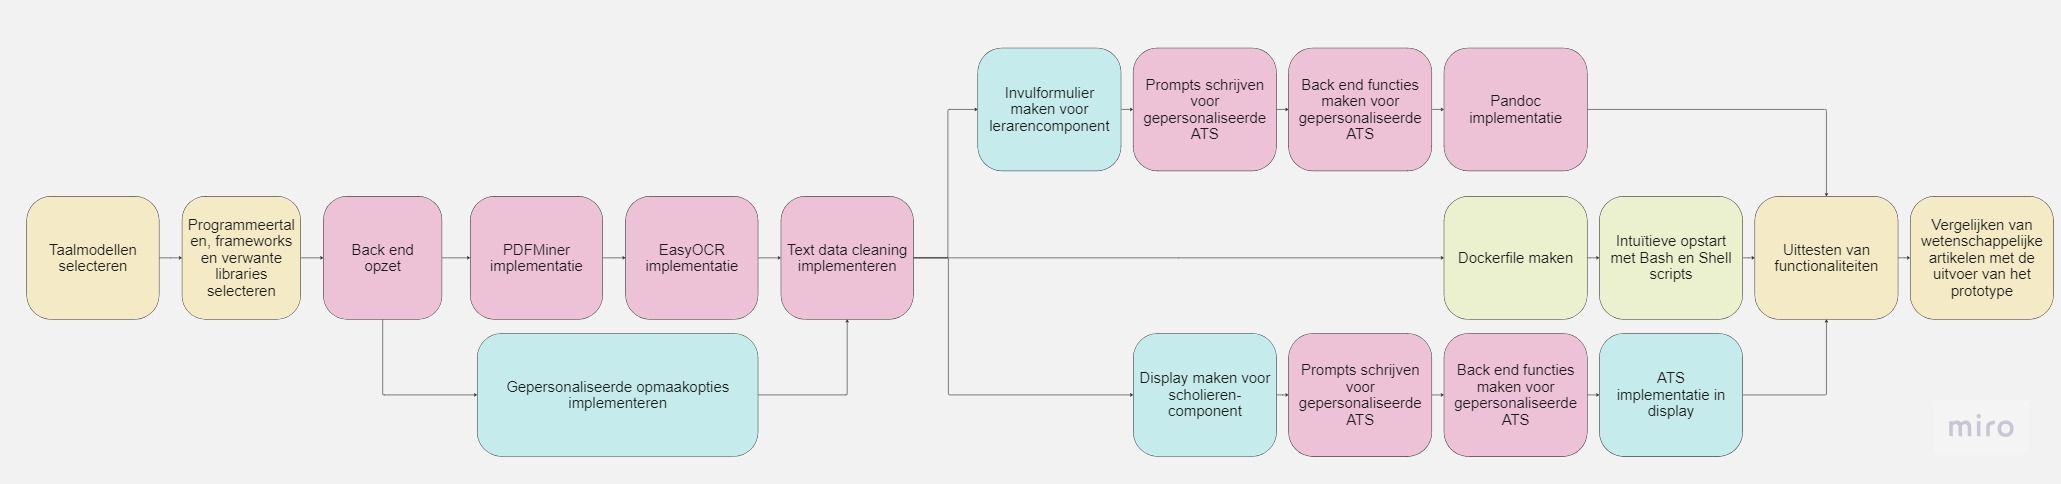
\includegraphics[width=\linewidth]{img/flowchart-general-development.jpg}
		\caption{Algemeen overzicht van de ontwikkeling van het prototype voor ATS van wetenschappelijke artikelen.}
		\label{img:general-overview-prototype}
	\end{figure}
\end{sidewaysfigure}

\subsubsection{Taalmodellen selecteren}

Allereerst bepaalt het onderzoek een taalmodel of meerdere taalmodellen voor gepersonaliseerde ATS, omdat deze keuze later de technologiekeuze kan beïnvloeden. Zo wijst het onderzoek uit dat GPT-3 een geschikt taalmodel is voor gepersonaliseerde ATS. Na de bepaling van het taalmodel bepaalt het onderzoek de technologieën en \textit{frameworks} voor de \textit{back end} en de \textit{front end}. 

\subsubsection{Programmeertalen, frameworks en verwante libraries selecteren}

Omwille van de beschikbaarheid van GPT-3 via API-calls, kunnen python en javascript geschikte keuzes voor dit prototype. Voor een snelle en gratis ontwikkeling gebruikt het prototype \textit{open-source} pakketten. Tabel \ref{table:technologies} toont een breed overzicht van alle gebruikte programmeertalen. Hierop vult tabel \ref{table:python-libraries} aan door een overzicht te geven van alle gebruikte python-libraries.

\begin{center}
	\begin{table}[H]
	\begin{tabular}{ | m{4cm} | m{11cm} | } 
		\hline
		\textbf{Technologie} 	& \textbf{Functionaliteit} \\
		\hline
		Python 					& De back end van het prototype die API-calls en de NLP-functionaliteiten zoals PoS-tagging en lemmatizing verwerkt. \\
		\hline
		JavaScript (JS)				& De toepassing gebruikersvriendelijker maken, personalisatie-opties voor de site doorvoeren en de functies gebouwd in Javascript dienen als alternatief op commandline instructies. \\
		\hline
		HTML en CSS 			& Het visuele uiterlijk van de website aanpassen naargelang de gekozen parameters van de eindgebruiker. \\
		\hline
		Jinja 					& Informatie uit de back end doorgeven aan de front-end.  \\
		\hline
		Docker 					& Lokale uitrol van de webtoepassing. \\
		\hline
		Bash					& Intuïtief script om de webtoepassing op te starten voor Linux en Mac-systemen. \\
		\hline
		Powershell 				& Intuïtief script om de webtoepassing op te starten op Windows-systemen. \\
		\hline
	\end{tabular}
	\caption{Gebruikte programmeertalen in het prototype voor tekstvereenvoudiging.}
	\label{table:technologies}
	\end{table}
\end{center}

\begin{center}
	\begin{table}[H]
	\begin{tabular}{ | m{4cm} | m{11cm} | } 
		\hline
		\textbf{Python-bibliotheek} & \textbf{Functionaliteit} \\
		\hline
		Flask					& Het framework van de webtoepassing. Dit framework combineert front end en back end. \\ 
		\hline
		PDFMiner 				& Tekstinhoud van PDF's extraheren. \\ 
		\hline
		EasyOCR					& PDF-pagina's inscannen als afbeelding in JPG-formaat om vervolgens de tekst te extraheren. \\
		\hline
		NumPy 					& De reshape-functie vereenvoudigt de manier om arrays van zinnen bij elkaar te plaatsen om zo een paragraaf te bekomen. \\
		\hline		
		Spacy 					& PoS-tagging en het lemmatiseren van woorden. \\
		\hline
		OpenAI					& GPT-3 API aanspreken. \\
		\hline
		BeautifulSoup			& HTML-content in het lerarencomponent \textit{parsen} voor een correcte formatting. \\
		\hline
	\end{tabular}
	\caption{Gebruikte Python-libraries en hun respectievelijke functie in het prototype.}
	\label{table:python-libraries}
	\end{table}
\end{center}

\subsubsection{Back end opzet}

Na het kiezen van de taalmodellen en de technologieën en frameworks, start het onderzoek met de front end implementatie. Allereerst voegt het onderzoek een homepagina toe dat als portaal zal dienen voor de leraren- en scholierencomponenten. Allereerst implementeert het onderzoek de nodige personaliseerbare opmaakopties. Zoals aangeraden door \textcite{Galliussi2020}, moeten ontwikkelaars rekening houden met de opmaakopties van de website. Zo maakt het prototype gebruik van alle parameters onderzocht door \textcite{Rello2013a, Rello2013b}. Het instellingenscherm is een HTML-bestand waarin een formulier alle aanpasbare parameters oplijst. Tabel ... toont de opgenomen parameters. De standaardparameters volgen de aangeraden parameters van (...). Het formulier stuurt vervolgens een POST-request naar de back end. De back end verwerkt deze aanvraag en slaat de ontvangen dictionary op als sessievariabele, zoals weergegeven in listing \ref{code:back-end-session-personalized}. 


\begin{lstlisting}[language=python, caption={De back end functie die de aanpassingen uit het formulier opslaat als sessievariabele.}, label={code:back-end-session-personalized}]
PER_SET_SESSION_NAME = 'personalized_settings'

@app.route('/get-settings-user',methods=['POST'])
def return_personal_settings_dict():
	if PER_SET_SESSION_NAME in session:
		return jsonify(session[PER_SET_SESSION_NAME])
	else:
		return jsonify(result='session does not exist')
	
@app.route('/change-settings-user', methods=['POST'])
def change_personal_settings():
	try:
		session[PER_SET_SESSION_NAME] = dict(request.form)
		msg = 'Succesvol aangepast!'
	except Exception as e:
		msg = str(e)
		flash(msg)
	return render_template('settings.html')
\end{lstlisting}

Tot slot moet de \textit{front end} deze opmaakopties bij iedere wegpagina inladen. Het inladen gebeurt met een \textit{window onload}, zoals weergegeven in listing \ref{code:window-onload-js}. Zo hoeven eindgebruikers deze parameters niet bij iedere webpagina opnieuw aan te passen.

\begin{lstlisting}[language=javascript, caption={De onload-functie die de gepersonaliseerde opmaakopties regelt bij het inladen van een webpagina.}, label={code:window-onload-js}]
window.onload = async function () {
	var url = `http://localhost:5000/get-settings-user`;
	const response = await fetch(url, { method: 'POST' });
	var result = await response.json();
	document.body.style.fontSize        = result.fontSize+'px';
	document.body.style.fontFamily      = result.fontSettings;
	document.body.style.backgroundColor = result.favcolor;
	document.body.style.lineHeight      = result.lineHeight+'cm';
	document.body.style.wordSpacing     = result.wordSpacing+'cm';
	document.body.style.textAlign       = result.textAlign;
}
\end{lstlisting}

Naast de gepersonaliseerde opmaakopties, moet het prototype ook over een systeem beschikken dat wetenschappelijke manieren kan opladen en inlezen. Zo biedt het prototype twee manieren aan om wetenschappelijke artikelen in te laten: via \textit{plaintext} of via een PDF-bestand. Niet alle \textit{PDF extractors} zijn foutbestendig, want zoals eerder opgemerkt in de \ref{sec:requirementsanalyse} kunnen \textit{PDF extractors} ook tekst verliezen tijdens dit proces. Als valnet biedt het prototype een OCR-optie aan. Deze functionaliteit omvat de ontwikkeling van functionaliteiten aan de front-end en aan de back end.

\medspace

De \textit{front end} kent enkel de toevoeging van een checkbox en twee \textit{input-tags}, namelijk een \textit{file-input} en een \textit{textarea-input}. De \textit{file-input} geeft de binaries van het PDF-bestand mee van de front-end naar de back end die het PDF-bestand tijdelijk \textit{in-memory} opslaat. Daarnaast krijgt de back end de keuze van de gebruiker tussen normale en OCR-upload mee als boolean, waarbij 1 gelijk staat aan een OCR-afhandeling. Uiteindelijk gebruikt het formulier een POST-request om alle meegekregen informatie door te sturen naar de back end. Na het ontvangen van de request van de front-end, handelt de Flask back end het bestand verder af zoals aangewezen in listing \ref{code:inlezen-wetenschappelijk-artikel-front-end-back-end}. Eerst controleert de \textit{back end} het type invoer. Vervolgens spreekt de Flask back end de Reader-klasse aan die de tekst formatteert tot een bruikbaar formaat voor de webtoepassing. Daarna gebruikt de Reader-klasse één van twee mogelijke technieken. 

\begin{lstlisting}[language=Python, caption={Koppeling tussen front-end en back-end voor het inlezen van een wetenschappelijk artikel}, label={code:inlezen-wetenschappelijk-artikel-front-end-back-end}]
def setup_scholars_teachers(request):
	settings = request.form
	if 'fullText' in request.form:
		text = request.form['fullText']
		langs = detect_langs(text)
		reader = Reader()
		dict_text = reader.get_full_text_site(text)                
	elif 'pdf' in request.files:
		if 'advanced' not in settings:
			pdf = request.files['pdf']
			pdf_data = BytesIO(pdf.read())
			all_pages = extract_pages(pdf_data,page_numbers=None,maxpages=999)
			langs = detect_langs(str(all_pages))
			reader = Reader()
			full_text = reader.get_full_text_dict(all_pages)
			dict_text = reader.get_full_text_site(full_text)
		else:
			pdf = request.files['pdf']
			pdf_data = pdf.read()
			pages = convert_from_bytes(pdf_data)
			reader = Reader()
			img_text = reader.get_full_text_from_image(pages)
			langs = detect_langs(img_text)
			dict_text = reader.get_full_text_site(img_text)                            
			return dict_text, langs, 'voorbeeldtitel', 'voorbeeldonderwerp'
			
@app.route('/for-scholars', methods=['GET','POST'])
def teaching_tool():
	try:
		dict_text, langs, title, subject = setup_scholars_teachers(request)
		return render_template('for-scholars.html', pdf=dict_text, lang=langs, title=title, subject=subject)
	except Exception as e:
		return render_template('error.html',error=str(e))
	
@app.route('/for-teachers', methods=['GET','POST'])
def analysing_choosing_for_teachers():
	try:
		dict_text, langs, title, subject = setup_scholars_teachers(request)
		return render_template('for-teachers.html', pdf=dict_text, lang=langs, title=title, subject=subject)
	except Exception as e:
		return render_template('error.html',error=str(e))
\end{lstlisting}

\subsubsection{PDFMiner implementatie}

Bij een gewone PDF-extractie gebruikt de Reader-klasse PDFMiner met de functie in listing \ref{code:inlezen-van-pdf}. Deze functie itereert doorheen alle PDF-pagina's van een meegekregen \textit{in-memory} pdf. Nadien extraheert de functie alle tekst op een pagina. Nadien concateneert deze functie alle opgehaalde tekst van één pagina aan een lege string. De functie herhaalt dit proces tot het script geen pagina's meer kan inlezen. Het resultaat van deze functie is een string-object met alle geëxtraheerde tekst uit een pdf.

\begin{lstlisting}[language=Python, caption={Een PDF inlezen met PDFMiner}, label={code:inlezen-van-pdf}]
	def get_full_text_from_pdf(self, all_pages):
		total = ""
		for page_layout in all_pages:
			for element in page_layout:
				if isinstance(element, LTTextContainer):
				for text_line in element:
					total += text_line.get_text()
					return total
\end{lstlisting}

\subsubsection{EasyOCR implementatie}

PDFMiner kan tekst missen bij de pdf-extractie. Daarom voorziet het prototype een valnet met een OCR-techniek. De Python-bibliotheek EasyOCR voorziet een eenduidige en ontwikkelaarsvriendelijke manier om tekst uit pdf's te extraheren met OCR-technieken. Zo itereert EasyOCR over alle pagina's in een PDF en slaat iedere pagina op als een JPG-bestand. Vervolgens leest EasyOCR de tekst op iedere pagina in en houdt dit bij tot het einde van het script. Na het inlezen van de tekst, verwijdert het script de aangemaakte afbeeldingen om zo geheugenruimte te besparen. Net zoals bij de eerste methode, resulteert deze methode in een string-object met alle tekst uit de PDF. De uitgewerkte code staat uitgeschreven in listing \ref{code:reader-ocr}

\begin{lstlisting}[language=Python, caption={Een PDF inlezen met OCR}, label={code:reader-ocr}]
	def get_full_text_from_image(self, all_pages):
		img_files = []
		num_pages = 0
		for i, page in enumerate(all_pages):
			file = f'page_{num_pages}.jpg'
			page.save(file, 'JPEG')
			img_files.append(file)
			num_pages += 1
		
		full_text = []
		reader = easyocr.Reader(['nl'])
		for f in img_files:
			result = reader.readtext(f, detail=0)
			full_text.append(" ".join(result))
			os.remove(f)
		return " ".join(full_text)
\end{lstlisting}

\subsubsection{Geëxtraheerde inhoud formatteren naar een webpagina.}

Na het extraheren van de tekstinhoud, komt een formatteerfase aan bod. Hier vormt het systeem de tekst om naar het gewenste formaat voor de front end. Allereerst transformeert de back end de string van geëxtraheerde tekst naar \textit{arrays} van zinnen met Spacy \textit{word embeddings} en \textit{sentence embeddings}. Deze functie staat beschreven in listing \ref{code:reader-formatting}. Het prototype bundelt vijf zinnen met de \textit{reshape-functie} van Numpy. Eindgebruikers kunnen deze parameter aanpassen in het instellingenscherm. Om de PoS-tag bij het respectievelijke woord bij te houden, gebruikt het prototype een \textit{key-value pair} datastructuur. Zo verwijst de sleutel naar een woord in een zin en de waarde verwijst naar de PoS-tag. Het prototype houdt rekening met enkel Nederlandstalige en Engelstalige wetenschappelijke artikelen. Daarom laadt het prototype hoogstens twee embeddingsmodellen op. Deze embeddingsmodellen staan vermeld in tabel \ref{table:wordembeddings-spacy}. Het prototype vermijdt hardcoderen. Daarom maakt het gebruik van een \textit{dictionary} die de naam van deze embeddingsmodellen bijhoudt. Het prototype gebruikt Engels als standaardtaal, als de back end de taal niet kan herkennen of als de taal niet in de lijst van de dictionary staat. 

\begin{lstlisting}[language=Python, caption={Het formatteren van de tekst naar een formaat voor de website.}, label={code:reader-formatting}]
	def get_full_text_site(self, full_text):
	try:
	lang = detect(full_text)
	except:
	lang = 'en'
	
	if lang in dict:
	nlp = spacy.load(dict.get(lang))
	else:
	nlp = spacy.load(dict.get('en'))
	
	full_text = str(full_text).replace('\n', ' ')
	
	doc = nlp(full_text)
	sentences = []
	for sentence in doc.sents:
	sentences.append(sentence)
	
	pad_size = SENTENCES_PER_PARAGRAPH - (len(sentences) % SENTENCES_PER_PARAGRAPH)
	padded_a = np.pad(sentences, (0, pad_size), mode='empty')
	paragraphs = padded_a.reshape(-1, SENTENCES_PER_PARAGRAPH)
	
	text_w_pos = []
	for paragraph in paragraphs:
	paragraph_w_pos = []
	try:
	for sentence in paragraph:
	dict_sentence = {}
	for token in sentence:
	dict_sentence[token.text] = str(token.pos_).lower()
	paragraph_w_pos.append(dict_sentence)    
	text_w_pos.append(paragraph_w_pos)
	except:
	pass
	return text_w_pos
\end{lstlisting}

Zowel het leraren- als het scholierencomponent passen deze dynamische HTML-structuur in hun weergave toe. Zo zijn er vier verschillende klassen die aan span-tags in deze weergave worden toegekend. Door middel van een Jinja-iteratie, krijgt iedere \textit{span-tag} een specifieke klasse afhankelijk van de key of iteratie. Deze iteratie toont listing \ref{code:html-span-tags} voor. Zo is er een overkoepelende span-tag \textit{sentence}, alsook voor ieder woord in een zin hoort er een span-tag met \textit{nouns}, \textit{adjectives} of \textit{verbs}. Andere woorden, zoals conjuncties, behoren tot de klasse \textit{other}. Na het extraheren van de tekstinhoud van een wetenschappelijk artikel, komt de ontwikkeling van het leraren- en scholierencomponent aan bod. Hoewel ontwikkelaars de ontwikkeling van beide componenten parallel kunnen laten lopen, start het onderzoek met de werkwijze voor de ontwikkeling van het lerarencomponent.

\begin{lstlisting}[language=html, caption={Het doorlopen van de PDF-tekst op de webpagina en het toekennen van de span-tags.}, label={code:html-span-tags}]

	<p class="left-side">
		
		<span class="sentence">
			
			
			<span class={{sentence[word]}}>{{word}}</span>
			
			
		</span>
	
	</p>

\end{lstlisting}


\subsubsection{Invulformulier maken voor het lerarencomponent.}

Zo kunnen leerkrachten beschikken over een tool waarin zij de geëxtraheerde tekstinhoud kunnen manipuleren, om vervolgens opties voor gepersonaliseerde ATS te selecteren. Figuur \ref{img:proto-lerarencomponent} toont een mogelijke weergave van deze HTML-pagina. Leerkrachten moeten in dit lerarencomponent kunnen beschikken over de functionaliteiten weergegeven in tabel \ref{table:functionaliteiten-leerkrachten}. Tabel \ref{table:criteria-requirementsanalysis} reikt de benodigde opties voor gepersonaliseerde ATS aan. Het prototype gebruikt deze criteria als opties om de prompts dynamisch op te bouwen.

\begin{center}
	\begin{table}[H]
		\begin{tabular}{ | m{7cm} | m{8cm} | } 
			\hline
			\textbf{Functionaliteit} & Gebruikte JS of python-techniek \\
			\hline
			Specifieke prompt meegeven per paragraaf & Naast een optie om voor het hele document één prompt te gebruiken, voegt het prototype ook een optie toe om. Hiervoor past de web-inhoud een key-value structuur toe. \\
			\hline
			Opties voor gepersonaliseerde ATS aanreiken. & Met behulp van een HTML-formulier kunnen leerkrachten opties aanvinken waaraan de vereenvoudigde tekst moet voldoen. \\
			\hline
			Werkwoorden, bijvoeglijke en zelfstandige naamwoorden markeren & Front-end aanpassing met \textit{eventlistener}. De tekstkleur van het aangeduide type woorden verandert naar het gekozen kleur. \\
			\hline
			Zinnen verwijderen & \textit{Front-end} filter aangesproken door een \textit{eventlistener}. \\
			\hline
			Woord toevoegen aan de woordenlijst & Een \textit{eventlistener} handelt de functionaliteit af. Het prototype slaat woorden en hun context tijdelijk op. Het formulier houdt dit bij en geeft het vervolgens mee bij het indienen. Deze woorden en hun respectievelijke zin van voorkomen dienen om de woordenlijst op te vullen in het gegenereerde PDF of Word-bestand. \\ 
			\hline 
		\end{tabular}
	\caption{Alle beschikbare functionaliteiten in }
	\label{table:functionaliteiten-leerkrachten}
	\end{table}
\end{center}

\subsubsection{Prompts schrijven voor gepersonaliseerde ATS in het lerarencomponent}

Het onderzoek stelt de prompts op volgens de richtlijnen beschreven in tabel \ref{table:techniques-for-good-prompts}. Daarnaast past het Intent- en Contextualization prompts toe zoals aangeraden door \textcite{White2023}. Tabel \ref{table:prompts-lerarencomponent} geeft een overzicht van alle opgestelde prompts die het prototype gebruikt in het lerarencomponent. Daarnaast gebruikt iedere API-call de parameters omschreven in tabel \ref{table:gpt-3-parameters-lerarencomponent}.

\begin{center}
	
\end{center}
\begin{table}[H]
	\begin{tabular}{ | m{5cm} | m{10cm} |}
		\hline
		\textbf{Functionaliteit} & \textbf{Prompt} \\ \hline
		Synoniem opzoeken & Geef een eenvoudiger synoniem voor '{woord}'. Context {context}. \\ \hline
		Definitie opzoeken & Geef een eenvoudige definitie voor '{woord}'. Context {context}.\\ \hline
		Zin vereenvoudigen & \\ \hline
		Gepersonaliseerde ATS & \\ \hline
		Gepersonaliseerde ATS als opsomming & Herschrijf dit als een lijst van vereenvoudigde zinnen met (gepersonaliseerde opties) :return: een lijst van vereenvoudigde zinnen gesplitst door een '|' teken /// {context}\\ \hline
	\end{tabular}
	\caption{Tabel met de gebruikte prompts voor het lerarencomponent.}
	\label{table:prompts-lerarencomponent}
\end{table}

\begin{center}
	\begin{table}[H]
		\begin{tabular}{| m{5cm}| m{10cm} |}
			\hline
			Parameter & Gebruikte waarde \\ \hline
			Prompt & Zie tabel \ref{table:prompts-lerarencomponent} \\ \hline
			Temperature & 0 \\ \hline
			Max tokens & De lengte van het woord vermeerdert met tien tokens als het over het opzoeken van een definitie of synoniem gaat. \\ 
			& Of de lengte van de zin vermeerdert met twintig tokens indien het over vereenvoudiging van een zin gaat. \\
			\hline
			Model & Da Vinci 3 \\ \hline
			Top-p & 90\% \\ \hline
			Stream & False \\ \hline
		\end{tabular}
		\caption{Gebruikte parameters om de definitie van een woord te genereren met GPT-3.}
		\label{table:gpt-3-parameters-lerarencomponent}
	\end{table}
\end{center}


\subsubsection{Back end functies maken voor gepersonaliseerde ATS}

Leraren kunnen handmatig zinnen uit de tekst verwijderen. Hiervoor gebruikt de \textit{front end} een \textit{eventlistener} die de aangeklikte span-tag van klasse 'sentence' uit het HTML-document verwijdert. Naast zinnen verwijderen kunnen leraren ook woorden aan een woordenlijst toevoegen. Hiervoor gebruikt de front-end een JS-script met een \textit{eventlistener} die een woord en de toebehorende zin toevoegt aan een \textit{textarea}. Deze \textit{textarea} gebruikt een \textit{pipe}-symbool als separator om nadien de text te splitsen en een array te bekomen. Om de leerkracht opties aan te reiken voor gepersonaliseerde ATS, bevat het HTML-document een formulier met keuzes aan. Dit formulier bevat alle nodige MTS-technieken uit tabel \ref{table:criteria-requirementsanalysis}. Na een POST-request krijgt de back end deze parameters die het systeem nadien verwerkt in de prompt voor het GPT-3 taalmodel. Leraren kunnen ook het uitvoerbestand personaliseren met lettertypes, gekozen regeleinde, woord-spatiëring en de marge van het document. Nadat de back end de inhoud van dit formulier ontvangt, neemt de GPT-klasse de aanvraag over. Deze klasse verwerkt drie functionaliteiten, namelijk definities en synoniemen opzoeken en gepersonaliseerde ATS.

\medspace

Allereerst dient de \textit{look-up} functie om de definitie van een woord te achterhalen. Zo beschrijft listing \ref{listing:gpt-look-up-word} de functie om met GPT-3 een eenvoudige definitie van een woord te genereren. Om de uitvoer zo waarschijnlijk mogelijk te maken, gebruikt de GPT-3 API-call een \textit{nultemperature}. Daarna haalt het script het verkregen antwoord uit de JSON-response om deze vervolgens tijdelijk bij te houden in een dictionary.

\begin{lstlisting}[language=Python, caption={Een functie om met GPT-3 een vereenvoudigde definitie voor een woord te genereren.}, label={listing:gpt-look-up-word}]
def look_up_word_gpt(self, word, context):
	try:
	prompt = f"""
	Give a simple Dutch explanation in one sentence for this word in the given context. Give the PoS-tag and Dutch definition: '{word}'
	context: {context}
	format: PoS-tag | definition
	"""

	result = openai.Completion.create(
	prompt=prompt,
	temperature=0,
	max_tokens=50,
	model=COMPLETIONS_MODEL,
	top_p=0.9,
	stream=False
	)["choices"][0]["text"].strip(" \n")    
	return result, word, prompt	
	except Exception as e:
	return 'error', str(e), str(e)
\end{lstlisting}

Vervolgens gebruikt de back end het GPT-3 model om een synoniem op te zoeken. Hiervoor spreekt de API de functie \textit{give-synonym} aan, verwezen in listing \ref{listing:gpt-give-synonym}.

\begin{lstlisting}[language=Python, caption={Een synoniem genereren of ophalen met GPT-3.}, label={listing:gpt-give-synonym}]
	""" @returns prompt, result from gpt """
	def give_synonym(self, word, context):
	try:
	prompt = f"""
	Give a Dutch synonym for '{word}'. If there is no Dutch synonym available, explain it between curly brackets.
	context:
	{context}
	"""
	
	result = openai.Completion.create(
	prompt=prompt,
	temperature=0,
	max_tokens=10,
	model=COMPLETIONS_MODEL,
	top_p=0.9,
	stream=False
	)["choices"][0]["text"].strip(" \n")    
	return result, word, prompt
	except Exception as e:
	return 'Open AI outage of problemen', str(e)
\end{lstlisting}
	
Daarna komt de vereenvoudiging van zinnen aan bod. Listing \ref{listing:gpt-personalised-simplify} bevat de code die deze API-call afhandelt. Echter moet het script rekening houden met twee aspecten. Allereerst kan de leerkracht kiezen voor een opsomming van de tekst. Daarnaast moet de inputlengte overeenstemmen met de beperkingen van de GPT-3 API. Wetenschappelijke artikelen zijn bijna altijd langer dan de mogelijk inputlengte. Daarom splitst het prototype de oorspronkelijke tekst op per 1000 tokens, zodat de inputprompt over marge beschikt en daardoor alle nodige gepersonaliseerde ATS-opties mee kan geven. Bij deze splitsing houdt het script rekening met de volledigheid van een zin. 
	
\begin{lstlisting}[language=Python, caption={Een zin gepersonaliseerd vereenvoudigen met GPT-3.}, label={listing:gpt-personalised-simplify}]
def personalised_simplify(self, sentence, personalisation):
	if 'summary' in personalisation:
		prompt = f"""
		Simplify the sentences in the given text and {", ".join(personalisation)}
		:return: A list of simplified sentences divided by a '|' sign
		///
		{sentence}
		"""
	else:
		prompt = f"""
		Explain this in own Dutch words and {", ".join(personalisation)}
		///
		{sentence}
		"""
	
	try:
		result = openai.Completion.create(
		prompt=prompt,
		temperature=0,
		max_tokens=len(prompt),
		model=COMPLETIONS_MODEL,
		top_p=0.9,
		stream=False
		)["choices"][0]["text"].strip(" \n")
		
		if 'summary' in personalisation:
			result = result.split('|')
		else:
			result = [result]
			
			return result, prompt
	except Exception as e:
		return str(e), prompt 
\end{lstlisting}


\subsubsection{Pandoc implementatie}

Ten slotte giet het script de \textit{plain-text} van vereenvoudigde tekstinhoud en de woordenlijsten in een pdf of docx-bestand. Zo maakt de Creator-klasse PDF's en docx-documenten volgens de meegegeven opmaakopties en maakt gebruik van Pandoc via python.  Pandoc gebruikt een tweestapsbeweging, waarbij het eerst \textit{plain-text} naar een markdownformaat omzet en vervolgens het Markdown-bestand naar een PDF of Word-document converteert. Daarvoor is een YAML-header nodig die de elementen, beschreven in tabel \ref{table:personalized-pdf-word-document-with-pandoc}, moet bevatten.

\begin{table}[H]
	\begin{tabular}{ | m{5cm}| m{10cm} | }
		\hline
		\textbf{Label in YAML-header} & \textbf{Voorbeeldwaarde} \\ \hline
		Title & Surveillance met artificiële intelligentie. \\ \hline
		Mainfont & Arial \\ \hline 
		Titlefont & Arial Black \\ \hline
		Date & 14-06-2023 \\ \hline 
		Document & Article \\ \hline
		Margin & 3cm \\ \hline
		Word-spacing & 0.3cm \\ \hline 
		Lineheight & singleheight \\ \hline
	\end{tabular}
	\caption{Benodigde labels voor een gepersonaliseerd document met Pandoc.}
	\label{table:personalized-pdf-word-document-with-pandoc}
\end{table}

Listing \ref{code:yaml-header-function} bouwt de YAML-header op voor het markdownbestand. Deze header is volledig parameteriseerbaar.

\begin{lstlisting}[language=Python, caption={Writer-klasse omvattende de code om dynamische PDF- en Word-documenten te genereren.}, label={code:yaml-header-function}]
	markdown_file = "saved_files/file.md"
	DATE_NOW = str(date.today())
	
	class Creator():
	def create_header(self, title, margin, fontsize, chosen_font, chosen_title_font, word_spacing, type_spacing):
		with open(markdown_file, 'w', encoding='utf-8') as f:
			f.write("---\n")
			f.write(f"title: {title}\n") 
			f.write(f"mainfont: {chosen_font}.ttf\n")
			f.write(f"titlefont: {chosen_title_font}.ttf\n")
			f.write(f'date: {DATE_NOW}\n')
			f.write(f'document: article\n')
			f.write(f'geometry: margin={margin}cm\n')
			f.write(f'fontsize: {fontsize}pt\n')
			f.write('header-includes:\n')
			f.write(f'- \spaceskip={word_spacing}cm\n')
			f.write(f'- \\usepackage{{setspace}}\n')
			f.write(f'- \{type_spacing}\n')
			f.write("---\n")
\end{lstlisting}

Om de woordenlijst aan het markdown-bestand toe te voegen, bouwt het script eerst een \textit{dictionary}-structuur op met de positie van het woord als key en als values de woord, de PoS-tag en de opgehaalde gepersonaliseerde betekenis. Het prototype moet rekening houden met homoniemen en daarom kan de key hier niet het woord zijn. Bij een lege woordenlijst komen deze bewerkingen niet aan bod. 

\begin{lstlisting}[language=Python, caption={Een woordenlijst genereren met de Writer-klasse.}, label={code:writer-glossary-klasse}]
def generate\_glossary(self, list):
with open(markdown_file, 'a', encoding='utf-8') as f:
f.write("---\n")
f.write("# Woordenlijst\n")
f.write("| Woord | Soort | Definitie |\n")
f.write("| --- | --- | --- |\n")
for word in list.keys(): 
f.write(f"| {word} | {list[word]['type']} | {list[word]['definition']} |\n")
\end{lstlisting}

Deze functie vult het markdown-bestand met de vereenvoudigde tekst, gesplitst door de titels die de leerkracht heeft gekozen. Het script slaat de vereenvoudigde tekst nadien op in een \textit{dictionary}-structuur. Vervolgens print het script de vereenvoudigde tekst uit naar het markdown-bestand door alle titels van de \textit{dictionary}-structuur te doorlopen. Een titel uitprinten in markdown syntax moet voorafgaan aan twee \textit{hashtags}, gevolgd door een \textit{breakline}. 

\begin{lstlisting}[language=Python, caption={Een doorlopende tekst toevoegen aan het markdownbestand met de Writer-klasse.}, label={code:writer-doorlopende-klasse}]
def generate_simplification(self, full_text):
with open(markdown_file,'a', encoding="utf-8", errors="surrogateescape") as f:
for key in full_text.keys():
title = str(key).replace('\n',' ')
text = full_text[key]
f.write('\n\n')
f.write(f'## {title}')
f.write('\n\n')
f.write(" ".join(text))
f.write('\n\n')
\end{lstlisting}

Indien de leerkracht een opsomming wenste, dan dient de titel nog steeds al separator, maar het script print de zinnen uit als opsomming conform aan de Markdown-syntax. Na de titel print het script de vereenvoudigde tekst per paragraaf uit. Bij een opsomming gaat een asterisk-symbool vooraf. Vervolgens converteert Pandoc het Markdown-bestand naar een PDF-bestand gebouwd met de XeLateX engine of een Word-bestand met de meegekregen binaries. 

\begin{lstlisting}[language=Python, caption={Een opsomming toevoegen aan het markdownbestand met de Writer-klasse.}, label={code:writer-summation-klasse}]
def generate_simplification_w_summation(self, full_text):
with open(markdown_file,'a', encoding="utf-8", errors="surrogateescape") as f:
for key in full_text.keys():
title = str(key).replace('\n',' ')
text = full_text[key][0].split('|')
f.write('\n\n')
f.write(f'## {title}')
for sentence in text:    
f.write('\n\n')
f.write(f'* {sentence}')
f.write('\n\n')
\end{lstlisting}

Tenslotte maakt het script de pdf en docx-bestanden van de vereenvoudigde teksten. De functie verwezen in listing \ref{code:writer-create-pdf} gebruikt alle bovenstaande (nodige) functies. Daarna genereert Pandoc de pdf en docx-bestanden. Nadien zal de functie deze twee bestanden comprimeren tot één zip-bestand. Hoewel Flask maar één bestand kan teruggeven, comprimeert het script met de \textit{zipfile} bibliotheek deze twee bestanden tot één bestand. Zo krijgt de eindgebruiker alsnog zowel het docx als het pdf-document. 

\begin{lstlisting}[language=Python, caption={Een zip-bestand aanmaken met daarin een docx en pdf bestand van de vereenvoudigde tekst.}, label={code:writer-create-pdf}]
def create_pdf(self, title, margin, list, full_text, fonts, word_spacing, type_spacing, summation):
if title is not None:
self.create_header(title=title, margin=margin, fontsize=14, chosen_font=fonts[0], chosen_title_font=fonts[1], word_spacing=word_spacing, type_spacing=type_spacing)
else:
self.create_header(title='Vereenvoudigde tekst', margin=0.5, fontsize=14, chosen_font=fonts[0], chosen_title_font=fonts[1], word_spacing=word_spacing, type_spacing=type_spacing)

"""GLOSSARY"""
if len(list) != 0:
self.generate_glossary(list=list)

"""SUMMARY"""
if summation:
self.generate_summary_w_summation(full_text=full_text)
else:
self.generate_summary(full_text=full_text)

"""FILE_CREATION"""
pypandoc.convert_file(source_file=markdown_file, to='docx', outputfile=docx_file,   extra_args=["-M2GB", "+RTS", "-K64m", "-RTS"])
pypandoc.convert_file(source_file=markdown_file, to='pdf',  outputfile=pdf_file,    extra_args=['--pdf-engine=xelatex'])
with zipfile.ZipFile(zip_filename, 'w') as myzip:
myzip.write(pdf_file)
myzip.write(docx_file)
\end{lstlisting}

De functionaliteiten van het lerarencomponent stoppen hier. Vervolgens komt het scholierencomponent aan bod, waarbij de nadruk ligt op het ontwikkelen van een ondersteunende tool.

\subsection{De ontwikkeling van het scholierencomponent.}

Tabel \ref{table:beschikbare-functionaliteiten-scholierencomponent} geeft een overzicht van alle functionaliteiten die in het scholierencomponent moeten zitten.

\begin{table}
	\begin{tabular}{| m{10cm} | m{5cm} |}
		\hline
		\textbf{Functionaliteit} & \textbf{JS/GPT-3} \\ \hline
		Zinnen verwijderen & Enkel JS \\ \hline
		Zinnen vereenvoudigen met gepersonaliseerde keuzes & GPT-3 en JS \\ \hline
		Zinnen vereenvoudigen met prompt & GPT-3 en JS \\ \hline
		Woord aan woordenlijst toevoegen & GPT-3 en JS \\ \hline
		Woorden (werkwoorden, bijvoeglijke en zelfstandige naamwoorden) markeren & JS \\ \hline
	\end{tabular}
	\caption{Beschikbare functionaliteiten in het scholierencomponent.}
	\label{table:beschikbare-functionaliteiten-scholierencomponent}
\end{table}

\subsubsection{Display maken voor scholierencomponent}

Net zoals bij het lerarencomponent, moet het prototype een oorspronkelijke weergave van het wetenschappelijk artikel kunnen tonen. Het onderzoek baseert de lay-out op dat van de erkende softwarepakketten, alsook de uitgeteste chatbots. 

\subsubsection{Prompts schrijven voor gepersonaliseerde ATS}

De prompts in tabel \ref{table:prompts-lerarencomponent} kan het scholierencomponent overnemen van het lerarencomponent. Aanvullend op deze prompts kunnen scholieren ook zelf een prompt schrijven.

\subsubsection{Back end functies schrijven voor gepersonaliseerde ATS}

Om zinnen in de doorlopende tekst te verwijderen, moet de front end over de nodige span-tags beschikken. Bij het inlezen van de PDF voert de back end dit al uit, zoals verwezen in listing \ref{code:reader-formatting}. Daarom hoeft het onderzoek geen nieuwe functie in de back end te schrijven. Vervolgens moet de back end over een functie beschikken om een zin te vereenvoudigen. Het lerarencomponent gebruikt al dergelijk functie. Daarmee hergebruikt de \textit{back end} de functie in listing \ref{listing:gpt-personalised-simplify}. 

\medspace

Zinnen baseren op een zelfgemaakte prompt moet de \textit{back end} echter wel toevoegen. Zo gebruikt de back end de functie in listing \ref{code:custom-prompt} om een \textit{custom prompt} te verwerken. Deze functie stuurt de oorspronkelijke prompt, samen met de context, door naar de GPT-3 API.

\begin{lstlisting}[language=python, caption={Een API-call sturen naar GPT-3 met een custom prompt.}, label={code:custom-prompt}]
def personalised_simplify_w_prompt(self, sentences, personalisation):
	try:
		result = openai.Completion.create(
			prompt=personalisation,
			temperature=0,
			max_tokens=len(personalisation)+len(sentences),
			model=COMPLETIONS_MODEL,
			top_p=0.9,
			stream=False
		)["choices"][0]["text"].strip(" \n")
		return result, personalisation
	except Exception as e:
		return str(e), personalisation
\end{lstlisting}

% 4.

Vervolgens heeft de back end als een functie die een woord opzoekt met GPT-3. Deze functie staat beschreven in listing \ref{listing:gpt-look-up-word} en de back end kan deze functie zonder problemen hergebruiken. Tot slot hoeft de \textit{back end} geen nieuwe functie te krijgen om woordmarkering af te handelen.

\subsubsection{Front end implementatie voor ATS functionaliteiten}

% 1.

Allereerst kan de \textit{front end} zonder hulp van de \textit{back end} zinnen met JS verwijderen. Alle woorden in een zin bundelt de front end in een span-tag van de klasse 'sentence'. Als de gebruiker dergelijk span-tag aanklikt, dan verwijdert de \textit{front end} de gekozen span-tag.

% 2.

Eerst slaat JS de gemarkeerde tekst en meegekregen ATS-opties op en geeft deze door aan de back end met een API-call. Vervolgens verwerkt de back end deze aanvraag door een nieuwe aanvraag te sturen naar GPT-3, met daarin een prompt die de tekst en de gekozen ATS-technieken bevat. De prompt specifieert het formaat waaraan de uitvoer van het taalmodel moet voldoen.  Als de tekst doorlopend is, dan verwerkt JS dit resultaat als een p-tag.  Als het taalmodel een opsomming moest genereren, dan zal de front-end alle zinnen doorlopen en uitprinten tussen twee li-tags.

% 3.

Listing \ref{code:frontend-add-word-to-glossary} toont de aanpak om via de front end een woord, pos-tag en definitie toe te voegen aan de woordenlijst tabel. De front end handelt enkel aanvragen voor werkwoorden, adjectieven, hulpwerkwoorden en zelfsandige naamwoorden af. Eenmaal de scholier op een woord drukt, stuurt de front end een aanvraag naar de back end. Hiervoor stuurt de front end de context en het woord naar de back end. De front end voegt nadien een nieuwe rij aan de tabel toe met daar in het woord, de PoS-tag en de definitie.

\begin{lstlisting}[language=javascript, caption={Een woord aan de woordenlijst toevoegen in het scholierencomponent.}, label={code:frontend-add-word-to-glossary}]
document.addEventListener("DOMContentLoaded", () => {
	const spans = document.querySelectorAll(".verb, .adj, .noun, .aux");
	spans.forEach((span) => {
		span.addEventListener("click", async (event) => {
			const radioButton = document.querySelector("#explainWords");
			if (radioButton && !radioButton.checked) {
				return;
			}
			let leftSideTag = span.closest("p");
			let rightSideTag = leftSideTag.nextElementSibling;
			sentence_of_origin = span.closest(".sentence");
			
			var context = "";
			for (const child of sentence_of_origin.children) {
				context = context + " " + child.textContent;
			}
			const word = event.target.textContent;
			const response = await fetch(`http://localhost:5000/look-up-word`, {
				method: "POST",
				headers: { "Content-Type": "application/json" },
				body: JSON.stringify({ word: word, sentence: context }),
			});
			result = await response.json();
			
			if (result.result == "error") {
				alert("Incorrect API key provided: " + result.word);
			} else {
				var pos_tag = result.result.split('|')[0];
				var definition = result.result.split('|')[1];
				let table = document.querySelector(".table-glossary");
				let newRow = table.insertRow(-1);
				let cell1 = newRow.insertCell(0);
				let cell2 = newRow.insertCell(1);
				let cell3 = newRow.insertCell(2);
				cell1.innerHTML = result.word;
				cell2.innerHTML = pos_tag;
				cell3.innerHTML = definition;
			}
		});
	});
});
\end{lstlisting}

% 4.

Tot slot moet de front end specifieke woorden kunnen markeren. De front-end beschikt al over de PoS-tags. Zo kan de front end, met de JS-functie in listing \ref{code:frontend-mark-pos-tag}, deze woorden een specifieke kleur geven als markering. De listing toont enkel het markeren van zelfstandige naamwoorden. Daarnaast kan de front end ook adjectieven uit de tekst verwijderen zonder taalmodel. Zo hoeft de JS-functie enkel de span-tags van de klasse 'adj' verwijderen uit de document.

\begin{lstlisting}[language=javascript, caption={Zelfstandige naamwoorden in het scholierencomponent markeren.}, label={code:frontend-mark-pos-tag}]
const nouns = document.getElementById('noun-show');

nouns.addEventListener('change', function () {
	if (this.checked) {
		const color = document.getElementById('colorForNouns').value;
		const elements = document.querySelectorAll("span.noun");
		elements.forEach(function (element) {
			element.style.color = color;
		});
	} else {
		const elements = document.querySelectorAll("span.noun");
		elements.forEach(function (element) {
			element.style.color = "black";
		});
	}
});
\end{lstlisting}

\subsection{De opzet voor een lokale webtoepassing.}

Via commandline kunnen eindgebruikers het prototype opstarten. Het prototype online plaatsen valt buiten de scope van dit onderzoek, maar Docker biedt wel een alternatief om een eenduidige opzet van het prototype te garanderen. Omdat het prototype enkel API's van taalmodellen aanspreekt, werkt het prototype met één Docker-container. Listing \ref{code:dockerfile} toont de gebruikte code van de Dockerfile. Voor het opstarten van de webapplicatie moet de Docker-container eerst de benodigde word-embeddings van Spacy installeren. Een scriptbestand in Powershell, zoals weergegeven in \ref{code:shell-boot}, of Bash zoals weergegeven in \ref{code:bash-boot}, maakt de opstart van deze webapplicatie intuïtiever dan via commandline. Het Pipreq-commando maakt een lijst van python-bibliotheken die Docker vooraf moet installeren. Voor een efficiënte ontwikkeling, moet de Docker-opzet pas laat in het ontwikkelproces gebeuren. Het requirements bestand moet alle nodige Python en front end packages bevatten. Dit proces als eerste laten verlopen kan de versies tegen het einde van de ontwikkeling gedateerd maken. Ten laatste moeten ook alle lettertypen zich in de lokale map bevinden, want Pandoc moet over alle lettertypen beschikken om een nieuw pdf of docx-bestand te kunnen maken.

\begin{lstlisting}[language=Dockerfile, caption={Dockerfile voor het prototype.}, label={code:dockerfile}]
	FROM python:3.8-slim-buster
	
	WORKDIR /app
	
	COPY requirements.txt requirements.txt
	
	RUN apt-get update && apt-get install -y pandoc texlive-xetex texlive poppler-utils
	
	RUN pip3 install -r requirements.txt \
	&& python3 -m spacy download nl_core_news_md \
	&& python3 -m spacy download en_core_web_md
	
	COPY . .
	
	CMD [ "python3", "-m" , "flask", "run", "--host=0.0.0.0", "--port=5000"]
\end{lstlisting}


\begin{lstlisting}[language=Powershell, caption={Script voor het opstarten van de Docker-container voor Windows-gebruikers}, label={code:shell-boot}]
	@echo off
	
	cd web-app
	docker stop text-application-prototype
	docker rm text-application-prototype
	
	docker rmi text-app
	
	docker build -t text-app .
	docker run --name text-application-prototype --network webapp_simplification -d -p 5000:5000 text-app
\end{lstlisting}

\begin{lstlisting}[language=Bash, caption={Script voor het opstarten van de Docker-container voor Unix-gebruikers}, label={code:bash-boot}]
	#!/bin/sh
	
	cd web-app || exit
	docker stop text-application-prototype
	docker rm text-application-prototype
	
	docker rmi text-app
	
	docker build -t text-app .
	docker run --name text-application-prototype --network webapp_simplification -d -p 5000:5000 text-app
\end{lstlisting}


\subsection{Experimenten en vergelijkende studie met het prototype.}

Het onderzoek rond de ontwikkeling van het prototype af met twee fasen. Het onderzoek achterhaalt of dit prototype voldoet aan twee zaken. Enerzijds achterhaalt het onderzoek of dit prototype voldoet aan de opgestelde functionaliteiten uit het moscow-schema, weergegeven in figuur \ref{img:moscow-table}. Daarmee toetst het onderzoek het prototype op basis van richtlijnen af. Nadien vergelijkt het onderzoek de functinonaliteiten met dat van andere toepassingen uit de requirementsanalyse. Ten laatste vergelijkt het onderzoek de aangemaakte wetenschappelijke artikelen, met de oorspronkelijke wetenschappelijke artikelen en referentieteksten door MTS.
\chapter{\IfLanguageName{dutch}{Resultaten}{Results}}%
\label{ch:resultaten}

In dit hoofdstuk worden de resultaten uit de requirementsanalyse, vergelijkende studie en de ontwikkeling van het prototype besproken. 

\section{Requirementsanalyse}

ChatGPT en Bing Chat zijn capabel om alle lexicale en syntactische vereenvoudigingstechnieken te realiseren. Tools, buiten Bing Chat en ChatGPT, zijn niet in staat om een formaatwijziging toe te passen. Enkel MTS is hiertoe voorlopig in staat, maar ChatGPT en Bing Chat maken gebruik van een technisch capabel taalmodel die deze taak kan realiseren. Het achterliggende taalmodel van beide tools is online via API beschikbaar. Daarmee is het aanbieden van gepersonaliseerde tekstvereenvoudiging bestaande uit lexicale, syntactische en structurele aanpassingen een \textit{must-have} voor prototype. Zoals uitgewezen in de literatuurstudie zijn er Python-libraries die dit realiseren, en daarmee vormt deze taak eveneens als een \textit{must-have} voor het prototype. Geen uitgeteste tool maakt gebruik van een personaliseerbare website. Daarop nog maken de uitgeteste sites weinig gebruik van de aangeraden aanschouwelijkheidsopties weergegeven in tabel \ref{table:dyslexia-necessaries}. Het prototype kan hiermee uitpakken en daarom vormt de personaliseerbare site als een \textit{must-have} voor het prototype. Om de tool te kunnen doorgeven aan vakexperten, wordt het prototype ook ontworpen met een lokale opzet in gedachten. Tools zoals Docker kunnen dit realiseren. Alle tools, buiten ChatGPT en Bing Chat, zijn in staat om een PDF met de vereenvoudigde tekstinhoud te genereren.

\medspace

Zowel Kurzweil3000 als Simplish bieden gegenereerde woordenlijsten aan, na de handmatige selectie van de gebruiker. Deze toevoeging is eerder ondersteunend, zoals aangewezen in tabel \ref{table:benefits-mts}. Daardoor is deze taak een \textit{should-have} voor het prototype. Zoals eerder aangehaald zijn tools in staat om een PDF te genereren, maar deze output is noch gepersonaliseerd noch heeft de eindgebruiker inbreng op hoe de uitvoer eruit moet zien. Open-sourcepakketten maken dit haalbaar en daarmee vormt deze taak een \textit{should-have}.

\medspace

Enkel Simplish en Rewordify bieden een ingebouwde tekstanalysemodele aan, zoals weergegeven in figuren \ref{img:simplish-output} en \ref{img:scholarcy}. Andere tools beschikken over geen leesgraadsmetrieken, noch van het ingegeven document, noch van het vereenvoudigde document. Simplish maakt gebruik van kleurcodecriteria om meer transparantie aan te reiken over de getransformeerde tekst, waaronder niet-veranderende woorden, adequate vertalingen, uitleg naar de voetnoot, homoniemen of woorden die geen eenvoudigere synoniemen hebben. Zoals aangegeven in figuur \ref{img:simplish-output} duidt de vergelijkende weergave de verschillen aan tussen de oorspronkelijke en vereenvoudigde tekst. Simplish beklemtoont de transformaties door middel van kleurcodes. Rewordify vult hierop aan en biedt meer inzichten in de leesbaarheidsgraad van de vereenvoudigde tekst, zoals geïllustreerd in figuur \ref{img:scholarcy}. Experimenten met Simplish en Rewordify wijzen uit dat dit een haalbare taak is, maar deze taak behoort niet tot prioriteit van het prototype en is daarmee een \textit{could-have}. Geen tool maakt gebruik van automatische selectie van moeilijke woorden, buiten ChatGPT en Bing Chat die dit enkel kunnen doen na een expliciete commando. ChatGPT en Bing Chat wijzen uit dat dit een haalbare taak is, mits het gebruik van een expliciete prompt, en daarom vormt deze taak een \textit{could-have} voor het prototype.

\medspace

De uitgeteste tools zijn allemaal online beschikbaar. Toch is dit onderzoek te kleinschalig om een volledig online beschikbare webtoepassing waar te maken en wordt deze taak als een \textit{wont-have} ingeschat. Daarmee blijft de opzet van de webtoepassing binnen een lokale omgeving. Ten slotte zijn de gebruikte tools of taalmodellen niet mogelijk binnen een lokale opzet. Zo is het GPT-3 model te groot om op een laptop lokaal te doen draaien. Daarom is de lokale hosting van het taalmodel een \textit{wont-have} voor het prototype. 

\section{Vergelijkende studie}

Na een tekstvereenvoudiging ligt het aantal zinnen bij T1, T2 en T3 hoger dan dat van de oorspronkelijke tekst. Elke prompt van T4 maakt gebruik van meer zinnen dan het oorspronkelijk artikel, zoals aangewezen in tabel \ref{table:resultaten-aantal-woorden}.

\medspace

T1, T2 en T3 gebruiken gemiddeld minder woorden per zin dan het oorspronkelijk artikel. Enkel P3 is in staat om gemiddeld minder woorden per zin te gebruiken, vergeleken met P1 en P2 die elk gemiddeld meer dan 19 woorden per zin gebruiken, zoals aangegeven in figuren \ref{img:boxplot-min-max-avg-words-a1} en \ref{img:boxplot-min-max-avg-words-a2}.

\medspace

De FRE-scores bij alle geteste taalmodellen en MTS-referentieteksten zijn niet significant hoger of lager, vergeleken met het oorspronkelijk wetenschappelijk artikel, zoals aangetoond in figuren \ref{img:boxplot-fre-a1} en \ref{img:boxplot-fre-a2}. Eveneens zijn de FOG-scores ook niet significant hoger of lager bij de vereenvoudigde wetenschappelijke artikelen zoals aangewezen in \ref{img:boxplot-fog-a1}, \ref{img:boxplot-fog-a2}.

\medspace

T1, T2 en T3 maken bij A1 en A2 gebruik van langere woorden ten opzichte van de oorspronkelijke tekst, in tegen stelling tot de drie T4 prompts die wel gebruik maken van kortere woorden en zo gelijkaardige resultaten bekomen als de MTS-referentieteksten. Deze verhouding wordt aangewezen in figuren 


% NB: all readability formulas were developed for English, so the scales of the outcomes are only meaningful for English texts. The Dale-Chall measure uses the original word list for English, but for Dutch and German lists of frequent words are used that were not specifically selected for recognizability by school children.


\subsubsection{Beoordeling op basis van referentieteksten en capaciteiten}

Taalmodellen T1, T2, T3 bieden geen opties voor gepersonaliseerde tekstvereenvoudiging. 

T1, T2 en T3 zijn niet in staat om syntactische vereenvoudiging op een tekst toe te passen. T3 is bij alle prompts in staat om de syntax van een zin te verlagen. Alle uitgeteste taalmodellen zijn echter wel in staat om lexicale vereenvoudiging te realiseren, al wordt de inschatting van de doelgroep in twijfel getrokken. De referentieteksten schatten de doelgroep correct in, door reeds gekend jargon niet aan te passen, maar nieuwe jargon wel aan te passen naargelang er een beschikbaar synoniem is. 

\medspace

De modellen T1, T2 en T3 zijn niet in staat om syntactische vereenvoudiging op een tekst toe te passen. Alleen T4 kan via de prompts P2, P3, P4, P5 en P6 de zinsstructuur verlagen. Hoewel alle geteste taalmodellen in staat zijn om lexicale vereenvoudiging te realiseren, wordt de nauwkeurigheid van de doelgroepsinschatting in twijfel getrokken. De referentieteksten schatten de doelgroep correct in door bekend jargon niet aan te passen, maar wel nieuwe jargon aan te passen als er een beschikbaar synoniem is.  Daarnaast kan T3-P1 ook de coherentie van een meegegeven paragraaf bevorderen, door onder meer omslachtige zinsstructuren aan te passen naar signaalwoorden. In tegenstelling tot GPT-3 zijn de modellen T1, T2 en T3 niet in staat om het formaat van de uitvoer aan te passen. De uitvoer blijft een doorlopende tekst. In de referentietekst past één van de auteurs het formaat aan naar tabelvorm voor enkele paragrafen, waar de inhoud beter in tabelvorm kan gestructureerd worden. Enkel prompts P5 en P6 wordt er expliciet gevraagd om een formaatwijziging, anders geeft T4 vrijwel altijd een doorlopende tekst terug. Zonder de expliciete aanduiding is het model niet in staat om dit zelf te bepalen. Verder onderzoek moet uitwijzen of T4 in staat is om zelfstandig deze bepaling kan maken, zo niet kan deze formaatwijziging niet automatisch bepaald worden en is er tussenkomst van de eindgebruiker vereist. Dit moet ook zo opgenomen worden als een functionaliteit in het prototype. Het formaat van de uitvoer bij de modellen T1, T2 en T3 zijn identiek aan dat van de oorspronkelijke tekst, namelijk in de vorm van een doorlopende tekst. Deze twee modellen zijn niet in staat om het voorbeeld van één van de auteurs te volgen, door formaatwijzigingen toe te passen. Eerder wees de requirementsanalyse uit dat T4 in staat is om met een expliciete prompt het formaat van de tekst aan te passen.

\medspace

De \textit{execution time} van T1 en T2 per API kan oplopen tot hoogstens 30 seconden voor een zin van tien tot dertig woorden, vergeleken met T3 die dezelfde zin in minder dan 10 seconden kan vereenvoudigen.

\section{Opbouw van het prototype}

Het prototype voldoet aan alle functionaliteiten die zijn gespecificeerd in het Moscow-schema \ref{img:moscow}. Het overtreft daarmee elke andere tool uit de requirementsanalyse op alle gebieden. Het is vooral op het gebied van formaatwijzigingen de beste, wat suggereert dat het prototype de huidige staat van deze toepassingen weergeeft, gezien de consistente ontwikkeling van de personalisatieopties. Op het gebied van tekstvereenvoudiging scoort het prototype vergelijkbaar of iets beter dan wat GPT-3 kan, wat voor zich spreekt aangezien het twee identieke taalmodellen zijn.

\medspace

Ontwikkelaars kunnen de opgebouwde flowchart volgen om team van vier rollen, namelijk systeem, data, NLP en web ontwikkelaars, te begeleiden doorheen de ontwikkeling van een toepassing voor tekstvereenvoudiging. De flowchart benadrukt dat deze handelingen ook perfect parallel kunnen worden uitgevoerd. Jupyter notebooks bieden een ontwikkelaarsvriendelijke manier om de code vooraf met eenduidige visuele feedback te kunnen testen.

\medspace

Dit prototype maakt geen gebruik van lokaal gehoste taalmodellen. Zo vermindert de nodige rekenkracht en geheugenruimte op het systeem waarop het prototype draait in vergelijking met een lokaal gehost taalmodel. Wanneer ontwikkelaars de toepassing willen uitrollen naar het grote publiek, kunnen ze overschakelen naar lokaal gehoste taalmodellen in plaats van taalmodellen per API. Door de taalmodellen verder te finetunen en te trainen op meer datasets, kunnen AI-ontwikkelaars betere resultaten behalen. 

\medspace

Het ontwikkelen van gebruikersvriendelijke handelingen kan gemakkelijk en snel worden ontwikkeld met behulp van HTML, CSS en JavaScript, zonder de nood van een complex framework. Uit onderzoek blijkt echter dat deze methoden eenvoudig te ontwikkelen zijn, zelfs door pas afgestudeerde bachelorstudenten. AI-softwarebedrijven zouden meer moeten inzetten op personalisatie-opties voor scholieren met dyslexie in de derde graad van het middelbaar onderwijs, omdat zij momenteel het meest betrokken zijn bij de digitalisering. Later kunnen softwareontwikkelaars overgaan op een complexer of robuuster framework. Verder onderzoek is nodig naar het ideale framework om een gepersonaliseerde weergave mogelijk te maken, aangezien dit momenteel nog wordt gedaan met handmatige JavaScript-functies. Een front-end framework dat dit alles beheert, zou handiger zijn voor webontwikkelaars.

\medspace

Dit prototype is momenteel alleen beschikbaar in een lokale omgeving en kan nog niet worden gebruikt door het grote publiek. Het prototype kan teksten lexicaal en syntactisch vereenvoudigen wanneer deze in PDF- of volledige tekstformaat worden ingevoerd. Het prototype heeft functionaliteit voor zowel docenten als studenten, die elk verschillende prioriteiten hebben. Hoewel testen nog nodig zijn, wordt dit wel aangeraden. Onderzoekers op het gebied van logopedie kunnen het prototype testen bij studenten met dyslexie na een (begeleide) installatie van de vereiste set-up. Ook onderzoekers op het gebied van onderwijs kunnen dit gebruiken om de meningen van zowel studenten als docenten te verzamelen en zo de effectiviteit van het prototype te beoordelen. Deze experimenten zijn belangrijk omdat ze kunnen wijzen op de effectiviteit van het prototype.


%%=============================================================================
%% Conclusie
%%=============================================================================

\chapter{Conclusie}%
\label{ch:conclusie}

Deze scriptie tracht een antwoord te bieden op de volgende onderzoeksvraag:

\begin{itemize}
	\item Hoe kan een wetenschappelijk artikel automatisch vereenvoudigd worden, gericht op de unieke noden van scholieren met dyslexie in de derde graad middelbaar onderwijs?
\end{itemize}

% ontbrekende mts en ontbrekende
Allereerst geeft de requirementsanalyse nieuwe inzichten in de huidige toepassingen voor ATS. Zo beschikken online tools te weinig over gepersonaliseerde ATS-functionaliteiten, zoals gebleken in sectie \ref{sec:requirementsanalyse}. Daarnaast maken geen tools buiten software specifiek voor scholieren met dyslexie geen gebruik van gepersonaliseerde opmaakopties. Toepassingen die wél wetenschappelijke artikelen kunnen opladen, beschikken over onvoldoende functionaliteiten om gepersonaliseerde ATS mogelijk te maken. Daarnaast ontbreken toepassingen die wél gepersonaliseerde ATS kunnen aanreiken over de nodige middelen om wetenschappelijke artikelen op een eenduidige manier op te laden. Om deze tools te kunnen gebruiken, moeten gebruikers \textit{commandline-interfaces} of chatbots gebruiken.

\medspace

% welk taalmodel gebruiken?
De vergelijkende studie wijst uit dat de geteste taalmodellen in staat zijn om LS mogelijk te maken. SS is enkel beschikbaar bij het GPT-3 model. Dit taalmodel kan doelgroepen in grote lijnen inschatten, alsook formaatwijzigingen toepassen zoals het herschrijven van een tekst als opsomming of in tabelvorm. Andere geteste HF-taalmodellen behalen zwakkere resultaten en vereisen een extra vertaalfase, die niet nodig is bij het aanspreken van de GPT-3 API.

\medspace

% hoe een prototype opzetten?
Uit de ontwikkeling van het prototype voor gepersonaliseerde ATS bleek dat \textit{open-source} AI en NLP-technologieën voldoende hoogstaand genoeg zijn om kwaliteitsvolle tekstvereenvoudigingssoftware te ontwikkelen. Zo kunnen ontwikkelaars gebruikmaken van PDFMiner om tekstinhoud uit wetenschappelijke artikelen te extraheren, van OpenAI's GPT-3 model via de API om gepersonaliseerde ATS mogelijk te maken en ten slotte van Pandoc om dynamische en gepersonaliseerde PDF-documenten automatisch te genereren. Binnen een webapplicatie kunnen eenduidige handelingen, gebouwd in JavaScript en HTML\&CSS, complexe commandlinehandelingen afhandelen.

\medspace

Ontwikkelaars hebben toegang tot T1, T2 en T3 via HuggingFace voor lexicale vereenvoudigingstaken. Deze taalmodellen zijn echter ontoereikend voor gepersonaliseerde tekstvereenvoudiging en daarom is T4 een geschikter model voor het vereenvoudigen van wetenschappelijke artikelen op maat. T4 presteert goed op gepersonaliseerde vereenvoudigingstaken, maar het is belangrijk om op te merken dat geen enkel taalmodel de doelgroep altijd nauwkeurig kan inschatten. Extra trainingsdata, zoals leerstof of wetenschappelijke artikelen die wel op het niveau van een 16-18-jarige zijn geschreven, kan het model steunen bij de doelgroepsinschatting. Het gebruik van Engelstalige prompts met expliciete vermelding van de gewenste uitvoertaal, resulteert in coherentere teksten dan bij een Nederlandstalige prompt.
%%=============================================================================
%% Discussie
%%=============================================================================

\chapter{\IfLanguageName{dutch}{Discussie}{Discussie}}%
\label{ch:discussie}

Dit onderzoek gebruikt drie onderzoeksmethoden om te bepalen hoe ontwikkelaars een optimale vorm van gepersonaliseerde ATS kunnen bieden aan scholieren met dyslexie in de derde graad van het middelbaar onderwijs.

\medspace

Uit de resultaten van de requirementsanalyse blijkt dat zowel erkende toepassingen als online tools onvoldoende functionaliteiten bieden voor gepersonaliseerde ATS. Daarnaast bieden deze tools onvoldoende gepersonaliseerde opmaakopties. Dit resultaat komt overeen met de verwachting dat bestaande tools niet specifiek gericht zijn op gepersonaliseerde ATS voor scholieren met dyslexie in de derde graad van het middelbaar onderwijs. Mogelijke verklaringen hiervoor zijn de populariteit van samenvattingstools in vergelijking met vereenvoudigingstools, de complexiteit die gepaard gaat met de ontwikkeling van dergelijke toepassing en het gebrek aan initiatief binnen dit vakgebied.

\medspace

Hoewel ChatGPT en Bing Chatbot functionaliteiten bieden voor gepersonaliseerde ATS, ontbreken eenduidige handelingen waardoor gebruikers moeite kunnen hebben met het vereenvoudigen van wetenschappelijke artikelen. Daarnaast houdt het model van ChatGPT geen rekening met verwijzingen of artikelen buiten de getrainde data, wat problemen kan veroorzaken voor data-integriteit. Hiertegenover staat Bing AI, dat wel rekening houdt met externe referenties en daarmee een goede basis vormt voor ontwikkelaars om referentiemateriaal aan te bieden in ondersteunende onderwijstoepassingen. Verder onderzoek naar de toepassing van deze AI via een API is noodzakelijk en kan baanbrekend zijn voor de onderwijssector. Aan de andere kant is er de mogelijkheid om bestaande toepassingen zoals Kurzweil uit te breiden met functionaliteiten die gepersonaliseerde ATS aanbieden aan scholieren met dyslexie in de derde graad van het middelbaar onderwijs.

\medspace

Vervolgens wijzen de resultaten van de vergelijkende studie uit dat het GPT-3 model geschikter is voor gepersonaliseerde ATS. Het geteste GPT-3-model gebruikt de davinci-engine en finetuned alleen API-parameters. Zo bevat het ook geen extra \textit{pre-trained} data van wetenschappelijke artikelen. De vergelijkende studie wijst verder uit dat de drie geteste HF-modellen via API en het geteste GPT-3-model via API beschikken over CWI-functionaliteiten en substitution generation. Hoewel de vrij beschikbare HF-taalmodellen LS mogelijk kunnen maken, staan ze in de schaduw van GPT-3, dat als API vrij beschikbaar is voor ontwikkelaars. Het GPT-3-model kan een baanbrekende oplossing bieden voor gepersonaliseerde ATS van wetenschappelijke artikelen, omdat het snel en efficiënt moeilijke woorden kan herkennen in doorlopende tekst en structurele aanpassingen kan maken aan de oorspronkelijke tekst.

\medspace

Dit resultaat bevestigt de verwachting dat GPT-3 beter in staat is om gepersonaliseerde ATS aan te bieden in vergelijking met vrij beschikbare HuggingFace-taalmodellen. Een verklaring hiervoor is de complexiteit van het taalmodel. Er zijn lichte verschillen in lexicale complexiteit tussen de HF-taalmodellen. Deze taalmodel zijn getraind op data van wetenschappelijke artikelen. Meer onderzoek is toch nodig om deze verschillen beter te begrijpen binnen de context van wetenschappelijke artikelen. De studie kon geen gebruikmaken van het opvolgende GPT-model, namelijk GPT-4, en hield geen rekening met het hoofdstuk waarin die een zin beoordeelt. Daarom bleven vragen over het verschil na ATS per hoofdstuk in een wetenschappelijk artikel onbeantwoord. Dit vereist verder onderzoek.

\medspace

LLM's, waaronder GPT-3, kunnen vragen beantwoorden en een eenduidige oplossing voor gepersonaliseerde ATS aanreiken aan ontwikkelaars. Er is onderzoek nodig naar de verschillen op taalgebied in relatie tot de toename van parameters bij grotere taalmodellen, zoals GPT-4. Er is behoefte aan onderzoek naar het gebruik van nieuwe modellen zoals GPT-4 en Bing AI in het onderwijs. Verder onderzoek naar de effecten van doelgroepinschattingen via prompts is ook nodig. Daarnaast zou toekomstig onderzoek zich kunnen richten op het potentieel van de combinatie van GPT-3 en textit{full-text-search}-technologieën. Onderzoek is nodig naar de verschillen tussen taalmodellen die getraind zijn op wetenschappelijke artikelen en taalmodellen die getraind zijn op algemene data binnen de context van wetenschappelijke artikelen. De verschillen tussen FRE en FOG waren onderling miniem. Tot slot wijst de vergelijkende studie uit dat de textit{readability}-library geen directe manier heeft om de actieve stem van een zin te achterhalen. Zo kan het onderzoek geen vaststelling maken of de uitgeteste taalmodellen in staat zijn om passief naar actief te schrijven. Spacy textit{word embeddings} kunnen een alternatieve manier aanreiken om hulpwerkwoorden en vervoegingen van het werkwoord zijn te achterhalen. Verder onderzoek is nodig om de bruikbaarheid van leesgraadscores te bepalen en te begrijpen hoe ze zich verhouden tot de kwaliteit van de vereenvoudigde tekst.

\medspace

Verworven kennis en aangeleerde tools uit alle richtingen Toegepaste Informatica aan Vlaamse Hogescholen, lieten toe om het prototype voor de webtool te ontwikkelen. Dit prototype dient slechts als een haalbaarheidstoetsing voor ontwikkelaars bij het ontwikkelen van dergelijke toepassing. Het is belangrijk dat de lezer zich bewust is van het feit dat de webtool zich baseert op onderzochte kenmerken en technieken die de impact van tekstvereenvoudiging met MTS hebben aangetoond bij scholieren met dyslexie. Daarnaast gebeurde de ontwikkeling van het prototype met het oog op een snelle en eenduidige implementatie van technieken die voordien enkel beschikbaar waren via CLI. Tijdens de ontwikkeling van het prototype is gebleken dat ontwikkelaars met vrij beschikbare middelen en API's in staat zijn om gepersonaliseerde ATS-toepassingen te bieden aan scholieren met dyslexie in de derde graad van het middelbaar onderwijs. Zo kunnen ontwikkelaars het stappenplan volgen om een vergelijkbaar resultaat te behalen en optioneel de taken in een projectteam parallel laten uitvoeren volgens de flowchart.

\medspace

Dit resultaat komt overeen met de verwachting dat ontwikkelaars over de benodigde tools beschikken om een dergelijk prototype voor gepersonaliseerde ATS te maken. Een verklaring hiervoor is de beschikbaarheid van textit{open-source} tools en python-bibliotheken die ontwikkelaars in staat stellen complexe taken eenvoudig uit te voeren. Toch moet de lezer zich ervan bewust zijn dat het prototype niet getest is bij het doelpubliek tijdens het begrijpend lezen van een wetenschappelijk artikel. Daarom kan het alleen dienen als een meting van de haalbaarheid voor ontwikkelaars. Er is een gebrek aan wetenschappelijke vakliteratuur over tekstvereenvoudiging met ATS voor deze doelgroep.

\medspace

Logopedisten of studenten in deze richting kunnen dit prototype gebruiken om onderzoek uit te voeren naar het effect op leesbegrip bij scholieren met dyslexie in de derde graad van het middelbaar onderwijs. Onderzoekers binnen het vakdomein secundair onderwijs kunnen de effecten van deze tool observeren bij leerlingen en leerkrachten in het middelbaar onderwijs. Er is echter meer onderzoek nodig om de inzet van gepersonaliseerde ATS-toepassingen en browserextensies voor tekstvereenvoudiging in het onderwijs te verbeteren. Er is behoefte aan een toepassing die alle functionaliteiten kan combineren. Bovendien is er behoefte aan meer onderzoek naar tekstvereenvoudiging met ATS voor de specifieke doelgroep van scholieren met dyslexie. Ten slotte is er onderzoek nodig naar de verbetering van de inzet van gepersonaliseerde ATS-toepassingen en browserextensies voor tekstvereenvoudiging in het onderwijs. Ook is er meer onderzoek nodig naar het gebruik van gepersonaliseerde ATS-toepassingen en browserextensies voor tekstvereenvoudiging bij scholieren met dyslexie in de derde graad van het middelbaar onderwijs.



%---------- Bijlagen -----------------------------------------------------------

\appendix

\chapter{Onderzoeksvoorstel}

\section*{Samenvatting}

% Kopieer en plak hier de samenvatting (abstract) van je onderzoeksvoorstel.
Ingewikkelde woordenschat en zinsbouw hinderen scholieren met dyslexie in het derde graad middelbaar onderwijs bij het lezen van wetenschappelijke artikelen. Gepersonaliseerde \textit{automated text simplification} (ATS) helpt deze scholieren bij hun leesbegrip. Daarnaast kan artificiële intelligentie (AI) dit proces automatiseren om de werkdruk bij leraren en scholieren te verminderen. Dit onderzoek achterhaalt met welke technologische en logopedische aspecten AI-ontwikkelaars rekening moeten houden bij de ontwikkeling van een AI-toepassing voor geautomatiseerde en gepersonaliseerde tekstvereenvoudiging. Hiervoor is de volgende onderzoeksvraag opgesteld: "Hoe kan een wetenschappelijk artikel automatisch worden vereenvoudigd, gericht op de unieke noden van scholieren met dyslexie in het derde graad middelbaar onderwijs?". Een requirementsanalyse achterhaalt de benodigde functionaliteiten om gepersonaliseerde en geautomatiseerde tekstvereenvoudiging mogelijk te maken. Vervolgens wijst de vergelijkende studie uit welk taalmodel kan worden ingezet om de taak van gepersonaliseerde en geautomatiseerde tekstvereenvoudiging mogelijk te maken. De requirementsanalyse wijst uit dat toepassingen om wetenschappelijke artikelen te vereenvoudigen, gemaakt zijn voor een centrale doelgroep en geen rekening houden met de unieke noden van een scholier met dyslexie in het derde graad middelbaar onderwijs. Toepassingen voor gepersonaliseerde ATS zijn mogelijk, maar ontwikkelaars moeten meer inzetten op de unieke noden van deze scholieren. 

% Verwijzing naar het bestand met de inhoud van het onderzoeksvoorstel
%---------- Inleiding ---------------------------------------------------------

\section{Introductie}%
\label{sec:introductie}

% TODO Bron voor de groei van python-pakketten toevoegen
België is een koploper in het gebruik van kunstmatige intelligentie (AI) op de werkvloer. Jaarlijks investeert de Vlaamse overheid 32 miljoen in het vakgebied \autocite{Crevits2022}. Zo zijn er verschillende projecten, om taalgerelateerde AI-ontwikkelingen op te starten, uit de grond gestampt. Het amai!-project \footnote{https://amai.vlaanderen/}  verenigt AI-softwarebedrijven uit verschillende domeinen en door hun inzet werden twee taaltoepassingen ontwikkeld voor het middelbaar onderwijs: \textit{real-time} ondertiteling en een taalassistent voor leerkrachten in meertalige klasgroepen. Het STEM-agenda\footnote{https://www.vlaanderen.be/publicaties/stem-agenda-2030-stem-competenties-voor-een-toekomst-en-missiegericht-beleid}
van de Vlaamse Overheid omvat aandachtspunten om het STEM-onderwijs tegen 2030 aantrekkelijker te maken door leraren, opleiders en begeleiders te ondersteunen. Het overbruggen van wetenschappelijke jargon is nergens in de aandachtspunten terug te vinden. STEM heeft echter een prominente rol binnen het onderwijs en de derde graad is een cruciale stap voor de verdere loopbaan van scholieren.

Dit onderzoek toont aan hoe de inhoud van wetenschappelijke artikelen door middel van kunstmatige intelligentie automatisch vereenvoudigd kan worden, specifiek gericht op de noden van scholieren met dyslexie in het derde leerjaar middelbaar onderwijs. Eerst vat het onderzoek samen wat tekstvereenvoudiging inhoudt en uit welke theoretische concepten dit bestaat. Vervolgens bespreekt het onderzoek hoe tekstvereenvoudiging en taalverwerking met AI scholieren met dyslexie van het derde graad middelbaar onderwijs kan helpen. Nadien staat het onderzoek stil bij de struikelblokken op taalvlak waarmee een tekstvereenvoudigingstoepassing rekening mee moet houden. Als volgt haalt het onderzoek aan welke tekstvereenvoudigingstoepassingen er nu in het onderwijs worden ingezet, welke internationale toepassingen teksten kunnen vereenvoudigen en hoe ontwikkelaars zelf een zelfgemaakte pipeline kunnen opbouwen. Ten slotte haalt het onderzoek de verschillende evaluatietechnieken aan die nodig zijn om de tekstinhoud na tekstvereenvoudiging te beoordelen, alsook aan welke ethische aspecten ontwikkelaars moeten denken bij het opzetten van een dergelijke. Het onderzoek eindigt met een vergelijkende studie van de aangehaalde toepassingen, waarbij de vereenvoudigde tekstinhoud subjectief en objectief wordt beoordeeld.

%---------- Stand van zaken ---------------------------------------------------

\section{State-of-the-art}%
\label{sec:state-of-the-art}

% Deelvraag: Wat is tekstsimplificatie
De voorbije tien jaar is artificiële intelligentie sterk verder ontwikkeld. De toename in kennis zorgde voor nieuwe toepassingen. Tekstvereenvoudiging vloeide hier uit voort. Momenteel bestaan er al robuuste applicaties voor tekstvereenvoudiging. Toch houdt de meerderheid niet genoeg rekening met het menselijk aspect van taalverwerking. Binnen het kader van tekstvereenvoudiging is er bestaande documentatie beschikbaar waar onderzoekers het voordeel van toegankelijkheid aanhalen, maar deze toepassingen ontbreken de extra noden die scholieren met dyslexie in het derde graad middelbaar onderwijs vereisen.

Het algemene doel van tekstvereenvoudiging is om ingewikkelde bronnen toegankelijker te maken. Het zorgt voor verkorte teksten zonder de kernboodschap te verliezen. Tekstvereenvoudiging \newline gebeurt doorgaans op één van drie manieren. Er is conceptuele vereenvoudiging waarbij documenten naar een compacter formaat worden getransformeerd. Daarnaast is er uitgebreide modificatie die kernwoorden aanduidt door gebruik van redundantie. Als laatste is er samenvatting die documenten verandert in kortere teksten met alleen de topische zinnen. Met deze concepten zijn ontwikkelaars in staat om ingewikkelde woorden te vervangen door eenvoudigere synoniemen of zinnen te verkorten zodat ze sneller leesbaar zijn \autocite{Siddharthan2014}.

Tekstvereenvoudiging behoort tot de zijtak van natuurlijke taalverwerking (NLP) in artificiële intelligentie. NLP omvat methodes om, door machinaal leren, menselijke teksten om te zetten in tekst voor machines. Documenten vereenvoudigen met NLP kan op twee manieren: extract of abstract. Bij extractieve simplificatie worden zinnen gelezen zoals ze zijn neergeschreven. Vervolgens bewaart een document de belangrijkste taalelementen om de tekst te kunnen hervormen. Deze vorm van tekstvereenvoudiging komt het meeste voor \autocite{Sciforce2020}. Daarnaast is er abstracte simplificatie die de kernboodschap van de zin bewaart en daarmee een nieuwe zin opbouwt. Volgens het onderzoek van \textcite{Chowdhary2020} heeft deze vorm potentieel dankzij de menselijke interpretatie, maar zit nog in de kinderschoenen.

% Deelvraag 2: Bewezen voordelen van tekstsimplificatie bij scholieren met dyslexie
Voor kinderen met dyslexie bestaan digitale hulpmiddelen die voor een betere visuele presentatie zorgen van teksten. Zo haalt het onderzoek van \textcite{Rello2012} tips aan waarmee teksten en documenten rekening moeten houden bij scholieren met dyslexie in het derde graad middelbaar onderwijs. Het gaat over speciale lettertypes, spreiding tussen woorden en het gebruik van inzoomen op aparte zinnen. Het onderzoek haalt aan dat teksten voor deze unieke noden aanpassen tijdrovend is, dus tekstvereenvoudiging door artificiële intelligentie kan een revolutionaire oplossing bieden. 

Het onderzoek van Franse wetenschappers \newline \textcite{Gala2016} illustreert dat manuele tekstvereenvoudiging schoolteksten toegankelijker maakt voor kinderen met dyslexie. Dit deden ze door simpelere synoniemen en zinsstructuren te gebruiken. Verwijswoorden werden vermeden en woorden kort gehouden. De resultaten waren veelbelovend. Het leestempo lag hoger en de kinderen maakten minder leesfouten. Ook bleek er geen verlies van begrip in de tekst bij geteste kinderen. Resultaten van de studie werden gebundeld voor de mogelijke ontwikkeling van een AI-hulpmiddel.

De Universiteit van Kopenhagen is met bovenstaande idee aan de slag gegaan. Onderzoekers \textcite{Bingel2018} hebben gratis software ontwikkeld, genaamd Hero\footnote{https://beta.heroapp.ai/}, om tekstvereenvoudiging voor scholieren in het middelbaar onderwijs met dyslexie te automatiseren. De software bestudeert met welke woorden de gebruiker moeite heeft, en vervangt die door simpelere alternatieven. Hero bevindt zich in beta-vorm en wordt enkel in het Engels en het Deens ondersteund. 

% Deelvraag: Waarop moet er gefixeerd worden bij een wetenschappelijke paper
\textcite{PlavenSigray2017} halen aan hoe onderzoekers in hun taalbubbel blijven, wat gevolgen voor de lezers met zich meebrengt. Daarnaast brengt de stijging aan het gebruik van acroniemen volgens \textcite{Barnett2020} een extra obstakel met zich mee. Het onderzoek van \textcite{Donato2022} wijst erop dat ondoorgrondelijke teksten te wijten zijn aan scholieren met dyslexie in het middelbaar onderwijs die uit hun richting vallen, wat voornamelijk bij STEM-richtingen het geval is. 

% Deelvraag: Uitdagingen van AI-software met tekstsimplificatie
NLP is de laatste decennia volop in ontwikkeling, maar ontwikkelaars botsen nog op uitdagingen. Het gaat om zowel interpretatie- als dataproblemen bij AI-machines. Allereerst is het voor een machine moeilijk om de context van homoniemen te achterhalen. Bijvoorbeeld bij het woord ‘bank’ is het niet duidelijk voor de machine of het gaat over de geldinstelling of het meubel. Daarnaast zijn synoniemen geen probleem voor tekstverwerking \autocite{Roldos2020}.

Het merendeel van NLP-toepassingen maakt gebruik van Engelstalige invoer. Niet-Engelstalige toepassingen zijn zeldzaam. De opkomst van AI-technologieën die twee datasets gebruiken, biedt een oplossing voor dit probleem. De software vertaalt eerst de oorspronkelijke tekst naar de gewenste taal, voordat de tekst wordt herwerkt \autocite{Sciforce2020}. Hetzelfde onderzoek bewijst dat het vertalen van gelijkaardige talen, zoals Duits en Nederlands, een minimaal verschil opleverd.

% Deelvraag: Stand van zaken bij Belgische secundaire scholen
De Vlaamse overheid leent gratis abonnementen uit voor voorlees- en schrijfsoftware, zoals \newline SprintPlus\footnote{https://www.sprintplus.be/}, Alinea\footnote{https://sensotec.be/product/alinea-suite/}, Kurzweil3000\footnote{https://sensotec.be/product/kurzweil-3000/}, TextAid\footnote{https://www.textaid-dyslexiesoftware.nl/textaid/} en Intowords\footnote{https://intowords.nl/}. Middelbare scholieren met dyslexie in het middelbaar onderwijs in België kunnen voor deze software een gratis abonnement of licentie aanvragen. Al bieden de vijf softwarepaketten elk een eigen samenvattingsfunctie, de focus ligt echter op spreek- en luistersoftware waarbij het samenvatten en markeren van tekst als extra wordt gehouden.

De sprong in AI gaf wereldwijd de aanzet om taalgerelateerde AI-toepassingen te ontwikkelen. ChatGPT\footnote{https://chat.openai.com/chat} van OpenAI is een chatbot met onder andere een simplificatiefunctie dat nu werkt op GPT-3, een API tegen aanbetaling. Nadelig moet de chatbot expliciet gevraagd worden om een bepaalde actie mogelijk te maken. Readable\footnote{https://readable.com/} is een online Engelstalige tool dat zinnen beoordeeld op basis van leesbaarheidsformules. Bij beide tools is het enkel mogelijk om tekst op de webpagina te plakken, dus er kunnen geen PDF-documenten of scans worden geüpload en eenzelfde werking verwachten. Op Nederlands vlak zijn er online verschillende samenvattingstools beschikbaar. Enkele voorbeelden zijn: Resoomer\footnote{https://resoomer.com/nl/}, Paraphraser\footnote{https://www.paraphraser.io/nl/tekst-samenvatting} en Prepostseo\footnote{https://www.prepostseo.com/tool/nl/text-summarizer}.

Vlaanderen heeft weinig zicht op de geïmplementeerde AI-software in scholen. Dit werd geconstateerd door \autocite{Martens2021}, een samenwerking tussen de Vlaamse universiteiten en overheid voor artificiële intelligentie. Vergeleken met andere Europese landen, maakt België het minst gebruik van leerling-georiënteerde hulpmiddelen. Degenen die wel gebruikt worden, zijn voornamelijk online leerplatformen voor zelfstandig werken. Ook maakt België amper gebruik van beschikbare software die de leermethoden en -noden van leerlingen evalueert \autocite{Martens2021a}. 

% Deelvraag: Wat is er nodig voor tekstsimplificatie? 
% Resultaat: Het ontwikkelen van een proof of concept pipeline met beschikbare word-embeddings en modellen
% Een pipeline voor een tekstsimplificatiepipeline omvat vijf fasen: Voor NLP-transformaties bestaan er talloze bibliotheken en kant-en-klare modellen die de logica achter deze stappen vereenvoudigen.

% Teksten samenvatten
% De kerninhoud van een tekst dient te allen tijde behouden te blijven. Bij het beoordelen van de correctheid van getransformeerde tekst met \textit{supervised} machinaal leren worden twee belangrijke metrieken gebruikt: ROUGE en BLEU. De berekening bij beide gebeurt op basis van overlappende n-grammen ofwel opeenvolgingen van tokens. ROUGE meet de overlappende n-grammen tussen getransformeerde en referentietekst. BLEU is een aangepaste versie van ROUGE gebruikt een precisie-gebaseerde scoringmethode met oog op niet alleen exacte, maar ook gedeeltelijke overeenkomsten. 

% Evaluatie
Om de transformatie van tekstvereenvoudiging te beoordelen, is er een tactvolle aanpak nodig. De studie van \textcite{Swayamdipta2019} haalt aan dat er extra nood is aan NLP-modellen waarbij de tekst zijn kernboodschap behoudt. Samen met Microsoft Research bouwden ze NLP-modellen die gericht waren op de bewaring van zinsstructuur en -context door \emph{scaffolded learning}. Hiervoor maakten de onderzoekers gebruik van een voorspellingsmethode die de positie van woorden en zinnen in een document beoordeelde.

Daarnaast wijst het onderzoek van \textcite{Readable2021} uit dat de Flesch-Kincaid leesbaarheidstest een objectieve manier aanbiedt om getransformeerde teksten te beoordelen. De leesbaarheidstest neemt drie factoren, namelijk zinlengte, woordfrequentie en complexiteit van het taalgebruik, en bepaalt hierop de moeilijkheidsgraad van een tekst. Deze score op Nederlandse teksten berekenen gebeurt eenvoudig met de Python-library textstat\footnote{https://pypi.org/project/textstat/}. 

\begin{figure}
	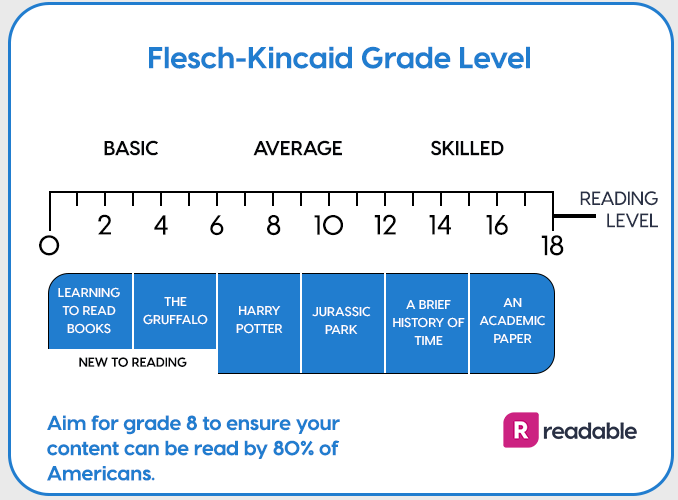
\includegraphics{img/Screenshot_302.png}
\end{figure}

% Bovendien zijn er kant-en-klare modellen die de complexiteit van tekst kunnen bepalen, hoewel deze beperkt zijn en vooral gericht zijn op Engelse teksten, zoals BERT\footnote{https://huggingface.co/docs/transformers/model\_doc/bert}, XLNet\footnote{https://huggingface.co/docs/transformers/model\_doc/xlnet}, GPT-3\footnote{https://platform.openai.com/docs/} en een open-source model genaamd TRUNAJOD\footnote{https://trunajod20.readthedocs.io/}.

%---------- Methodologie ------------------------------------------------------
\section{Methodologie}%
\label{sec:methodologie}

% wat is tekstsimplificatie - welke soorten tekstsimplificatie 
% hoe bevoordeelt het aan scholieren met dyslexie in het derde graad secundair - wat zijn de struikelblokken
% welke software wordt er momenteel ingezet + vrij beschikbare software
% opbouw van een tekstsimplificatiepipeline + evaluatietechnieken
Het onderzoek houdt zeven fases in. De eerste fase is het proces van tekstvereenvoudiging beschrijven, waaronder een omschrijving van het begrip en de verschillende soorten van technologische tekstvereenvoudiging. Dit gebeurt via een grondige studie van vakliteratuur en wetenschappelijke teksten. Ook blogs van experten komen hier aan bod. Na het verwerven van de nodige inzichten wordt er een verklarende tekst opgesteld.

De tweede fase bestaat uit het analyseren van wetenschappelijke werken over de bewezen voordelen van tekstvereenvoudiging bij scholieren met dyslexie van het derde graad middelbaar onderwijs. Hiervoor zijn geringe thesissen beschikbaar, die zorgvuldigheid vragen tijdens interpretatie. De resulterende tekst bevat de voordelen samen met hun wetenschappelijke onderbouwing.

De derde fase is het verzamelen van alle nodige transformaties om een wetenschappelijke paper beter leesbaar te maken voor een scholier met dyslexie in het derde graad middelbaar onderwijs. Het resultaat is een shortlist van alle evaluatiecriteria waaraan de uitvoertekst van een tekstvereenvoudigingstoepassing moet voldoen.

De vierde fase is opnieuw een beschrijving. Hier worden de valkuilen bij taalverwerking met AI-software nagegaan. Deze fase van het onderzoek brengt mogelijke nadelen en tekortkomingen van AI-software bij tekstvereenvoudiging aan het licht. Dit gebeurt aan de hand van een technische uitleg.

De vijfde fase omvat een toelichting en advies over de beschikbare Nederlandstalige AI-tools voor tekstvereenvoudiging. Aan de hand van een veldonderzoek op het internet en bij bedrijven wordt er op zoek gegaan naar dergelijke software. Er wordt niet gezocht naar vertaalsoftware of toepassingen die de inhoud van een afbeelding of tekstbestand omzet naar tekstinhoud.

De zesde fase omschrijft een technisch uitwerking van een tekstvereenvoudigingspipeline, alsook een shortlist van metrieken om de tekstvereenvoudiging te evalueren. Er zal een tekstvereenvoudigingspipeline worden ontwikkeld met beschikbare kant-en-klare bibliotheken, \textit{transformers} en algoritmes. Het resultaat van deze fase is een pipeline opgebouwd in de programmeertaal Python. 

De zevende en laatste fase omvat een vergelijkende studie van de gevonden tekstvereenvoudigingstoepassingen, alsook de tekstvereenvoudigingspipeline. Wetenschappelijke papers, die in een derde graad middelbaar onderwijs worden gebruikt, dienen hier als invoertekst voor de evaluatie. De transformatie wordt met zowel objectieve als subjectieve metrieken beoordeeld. De subjectieve test gebeurt aan de hand van een \textit{survey} en een \textit{think-aloudtest}. De objectieve testen gebeuren op basis van de shortlist uit de derde fase en de shortlist van metrieken uit de zesde fase. Ten slotte volgt er een persoonlijk advies over de nodige ontwikkelingen in het vak op vlak van Nederlandstalige tekstvereenvoudiging.

%---------- Verwachte resultaten ----------------------------------------------
\section{Verwacht resultaat, conclusie}
\label{sec:verwachte_resultaten}

Er wordt verwacht dat de software, die momenteel in het onderwijs wordt ingezet, niet voldoet aan de noden van een scholier met dyslexie in het derde graad middelbaar onderwijs. Dit is omdat er onvoldoende rekening wordt gehouden met hun unieke uitdagingen. Het vertalen van de outputtekst bij een internationale AI-tool zal mogelijk afwijken van de oorspronkelijke context. 

Er zijn onvoldoende kant-en-klare algoritmen en modellen beschikbaar om een tekstsimplificatiepipeline, waarvan de output verzorgd is aan de unieke noden van een scholier met dyslexie in het derde graad middelbaar onderwijs, te bouwen. De pipeline vergt \textit{custom transformers} om nauwkeurige resultaten te bekomen, zodat de kerninhoud niet verloren raakt. Het vertalen van de zinnen verlaagt de nauwkeurigheid van het model, maar is een acceptabel alternatief. Er is nood aan Nederlandstalige \textit{word embeddings} die de complexiteit per woord bijhouden, alsook meer kant-en-klare modellen die tekstsimplificatiefuncties aanbieden.

%%---------- Andere bijlagen --------------------------------------------------
\chapter{Algemene richtlijnen}
	
Het onderzoek achterhaalt hoe scholieren met dyslexie in de derde graad middelbaar onderwijs ondersteund kunnen worden bij het intensief lezen van een wetenschappelijk artikel. De ondersteuning wordt aangeboden in de vorm van tekstvereenvoudiging met AI. Tekstvereenvoudiging omvat het lexicaal en syntactisch vereenvoudigen, alsook het samenvatten van de kerngedachte per hoofdstuk. Om tekstvereenvoudiging met AI te testen, moeten handmatig en automatisch vereenvoudigde teksten met elkaar worden vergeleken. 
	
	\medspace
	
De opdracht voor deze bijdrage is het manueel vereenvoudigen van een gekregen wetenschappelijk artikel. Dit wetenschappelijk artikel is zes pagina's (voorpagina uitgesloten) lang. Het doelpubliek voor dit vereenvoudigd artikel zijn scholieren met dyslexie in de derde graad ASO/TSO middelbaar onderwijs. Concreet zou dit een artikel moeten zijn dat tijdens een STEM-les wordt gegeven aan deze doelgroep. Op pagina 2 vindt u tekstvereenvoudigingstechnieken terug. Deze aanpassingen hebben een beneficieel effect op scholieren met dyslexie een wetenschappelijk artikel bij het intensief lezen van wetenschappelijke teksten. U dient deze gekregen aanpassingen te volgen voor deze bijdrage. De beschreven technieken en elementen dienen in de manuele vereenvoudigde tekst terug te vinden zijn. 
	
	\medspace
	
Op basis van de richtlijnen op pagina 2 worden dezelfde instructies aan een AI-model gegeven. Met de richtlijnen en de door u handmatig vereenvoudigde tekst kan het onderzoek evalueren of AI-taalmodellen capabel zijn om manuele tekstvereenvoudigingstechnieken, specifiek voor scholieren met dyslexie, toe te passen op wetenschappelijke artikelen. De tekst dat een AI-model vereenvoudigd wordt afgetoetst op basis van bestaande metrieken en de kenmerken van uw vereenvoudigde versie. % Woordenschat die in de eerste en tweede graad gekend zijn, hoeven niet aangepast te worden en wordt vernomen als 'gekend'. 
	
	\medspace
	
Voor de vereenvoudigde versie van het artikel moet u als taaldocent of auteur geen rekening houden met marges, lettertypes of spatiëring. Deze aanpassingen mogen, maar enkel de tekstuele inhoud van het gekregen document wordt in het experiment opgenomen. Een Word-document of PDF-document is voldoende. Daarnaast moet er ook geen rekening worden gehouden met de afbeeldingen in het artikel.  
	
	\medspace
	
Aanpassingen die niet op pagina 2 omschreven zijn om de tekst eenvoudiger te maken, zijn vrijblijvend. Indien deze aanpassing volgens u een meerwaarde biedt, dan moet de werkwijze voor de start van het document kort beschreven worden. De aanpassing moet eenmalig bovenaan het document worden vermeld. Bijvoorbeeld: 'De zin werd gesplitst omdat deze langer is dan tien woorden.' Zo kunnen wij bij het onderzoek rekening houden met deze extra handeling. Het AI-model wordt dan met deze extra parameter in het achterhoofd beoordeeld.
	
	\medspace
	
Namens mijn promotor, copromotors en mezelf wil ik u hartelijk bedanken voor uw interesse in dit onderzoek.
	
	\newpage
	
\subsection{Lexicale vereenvoudiging}
	
\begin{itemize}
	\item Een moeilijk woord achterhalen gebeurt op basis van intuïtie en inschatting van de doelgroep. De woordenschat die zelden voorkomt in de dagelijkse lees- en schrijftaal van STEM-vakken voor scholieren tussen 16 en 18 jaar oud, moet worden aangepast. Vakjargon die al in de tweede graad ASO en TSO aan bod is gekomen, mag behouden blijven.
	\item Een woord dat langer is dan achttien letters, wordt als moeilijk beschouwd en moet vervangen worden door een korter (en eenvoudiger) alternatief.
	\item Acroniemen worden voluit geschreven.
	\item Vervang een moeilijk woord in het artikel door slechts één synoniem. Bijvoorbeeld, als het woord 'adhesief' wordt vervangen door 'klevend', gebruik dan geen andere synoniemen voor 'klevend' in de rest van het artikel. 
	\item Indien een woord geen eenvoudiger synoniem heeft, mag het woord kort worden uitgelegd. Dit kan tussen ronde haakjes, of in een aparte zin. Bijvoorbeeld: "Ik voelde me melancholisch." wordt aangepast naar "Ik had een diep gevoel van droefheid en verlies.".		
		\item Vermijd het directe overnemen van percentages indien deze voorkomen in het artikel. Vervang dit door benamingen zoals 'een kwart', 'de helft'. 
	\end{itemize}
	
	\subsection{Syntactische vereenvoudiging}
	
	\begin{itemize}
		\item Te lange zinnen worden opgebroken of gesplitst. De zinnen in het vereenvoudigde artikel zijn hoogstens tien woorden lang.
		\item Verwijswoorden zoals 'zij', 'hun' of 'hij' worden naar namen veranderd. Bijvoorbeeld voornamen of entiteitsnamen (bijvoorbeeld Nationale Bank). 
		\item Tangconstructies worden vervangen. Dit kan door de bijzin naar het begin of het einde van een zin te plaatsen, de zin te splitsen in twee kortere zinnen of door het onderwerp en de persoonsvorm dichter bij elkaar te plaatsen door minder informatie tussenin te plaatsen.
		\item Voorzetseluitdrukkingen en samengestelde werkwoorden worden vervangen indien mogelijk. Indien er geen eenvoudigere alternatieven zijn, mogen deze onaangepast blijven.
	\end{itemize}
	
	\subsection{Samenvatten}
	
	\begin{itemize}
		\item Het vereenvoudigde artikel volgt dezelfde structuur en chronologische volgorde zoals dat van het oorspronkelijk artikel. Iedere hoofdstuk in het wetenschappelijk artikel is hoogstens twee paragrafen lang. Per paragraaf zijn er hoogstens vijf zinnen.
		\item Het vereenvoudigd artikel is hoogstens 500 woorden lang. 
		\item Citeren mag indien deze zinnen aan de bovenstaande criteria (lexicale en syntactische vereenvoudiging) voldoen.
		\item Het gebruik van opsommingen of \textit{bullet-points} wordt aangemoedigd.
		\item De bronvermelding wordt overgenomen. De referentie gebeurt zoals die uit het oorspronkelijke document (Vancouver) en mag direct overgenomen worden: '[4]' blijft '[4]'.
	\end{itemize}
	
	
	\section{Specifieke richtlijnen voor A1}
De kerngedachte van iedere paragraaf moet terug te vinden zijn in de vereenvoudigde tekst. Na de tekstvereenvoudiging moeten de volgende vragen in hoogstens twee paragrafen beantwoord kunnen worden:
	
	\begin{itemize}
		\item \textbf{Inleiding}: Wat is het doel van dit onderzoek? Uit welk eerder onderzoek of uit welke probleemstelling vloeide dit onderzoek voort?
		\item \textbf{Socio-technische ontwikkeling}: Welke drie technische ontwikkelingen worden aangehaald in het onderzoek? Wat zijn de sociotechnische ontwikkelingen die het traditionele controle- en handhavingskader onder druk zetten als gevolg van de opkomst van algoritmische surveillance in het politiewerk?
		\item \textbf{Juridisch kader}: Wat zijn de tekortkomingen van het huidige juridisch kader en de controle-instrumenten die momenteel worden ingezet voor de verwerking van gegevens door middel van AI, en biedt het recente voorstel van de EU voor een AI-wet voldoende bescherming van grondrechten en handhavingsmechanismen?
		\item \textbf{Herdenken van algoritmische surveillance-controle}: Hoe kan de visie van Ubuntufilosofie en relationele ethiek bijdragen aan een herziening? Hoe kan relationele controle helpen bij het beschermen van kwetsbare groepen tegen schendingen van mensenrechten door algoritmische surveillance?
		\item \textbf{Concrete stappen}: Welke concrete stappen omtrent ethiek worden er aangehaald? Hoe kan relationele controle helpen bij het herdenken van controlemechanismen en rekening houden met sociaal-technische ontwikkelingen zoals asymmetrische machtsrelaties en de toenemende macht van technologiebedrijven?
		\item \textbf{Conclusies}: Wat besluiten de onderzoekers? Indien verder onderzoek vereist is, naar welk onderzoek kijken ze specifiek uit?
	\end{itemize} 


\section{Specifieke richtlijnen voor A2}

Het doel is om de kerngedachte van iedere paragraaf in de vereenvoudigde tekst terug te kunnen vinden, alsook een antwoord moet kunnen geven op de onderstaande vragen per sectie. Enkel de doorlopende tekst moet worden vereenvoudigd, dus geen extra uitleg over de grafieken en visualisaties. Daarnaast moet de vereenvoudigde tekst een antwoord kunnen geven op de vragen in hoogstens vier paragrafen beantwoord kunnen worden:

\begin{itemize}
	\item \textbf{Inleiding}: Wat is de probleemstelling voor dit onderzoek? Welk doel heeft deze bijdrage? Opmerking: uitzonderlijk moet deze sectie tot hoogstens één paragraaf worden samengevat.
	\item \textbf{Beleidsaanpak}: 
	\begin{itemize}
		\item Welke economische problemen zijn er ontstaan als gevolg van de oliecrisissen en invoerconcurrentie in Nederland en België?
		\item Wat waren de belangrijkste beleidswijzigingen? Welke gevolgen waren er?
		\item Wat zijn de belangrijkste verschillen tussen de Nederlandse en Belgische economie en wat zijn de belangrijkste uitdagingen waar deze landen momenteel voor staan?
		\item Hoe verschillen de aanpak en uitgaven van de overheid in België en Nederland en wat zijn de gevolgen daarvan voor hun economieën en overheidsfinanciën?
	\end{itemize}
	
	\item \textbf{Competitiviteit}
	\begin{itemize}
		\item Welke factoren hebben geleid tot het verschil in economische prestaties tussen Nederland en België, en wat is de rol van de werkzaamheidsgraad in deze verschillen?
		\item Wat zijn de belangrijkste redenen voor het verschil in groeiprestaties tussen Nederland en België, en welke factoren spelen hierbij een rol, met name op het gebied van arbeidsmarkt, innovatie en ondernemerschap?
		\item Welke observaties worden er gemaakt over ondernemerschap en innovatie in Nederland en België?
		\item Wat is het verband tussen de inkomende en uitgaande buitenlandse directe investeringen als percentage van het BBP en de internationalisatie van bedrijven in Nederland en België?
	\end{itemize}
	\item \textbf{Structurele evoluties in beide landen}:
	\begin{itemize}
		\item Welke factoren hebben geleid tot de de-industrialisatie in België en Nederland en welke impact heeft dit gehad op de werkgelegenheid en productiviteit in beide landen?
		\item Hoe beïnvloedt de ongelijke groei tussen de dienstensector en de industriële sector de productiviteit en de economische groei in België?
		\item Hoe verschilt de dynamiek van de drie gewesten in België met betrekking tot de economische bevoegdheden en de neerwaartse convergentiekrachten in de EU?
	\end{itemize}
	Opmerking: Er worden hier drie vragen gesteld, maar u mag nog steeds hoogstens vier paragrafen gebruiken om deze sectie samen te vatten en te vereenvoudigen.
	\item \textbf{Conclusies}: Wat besluiten de onderzoekers?  Indien verder onderzoek vereist is, naar welk onderzoek kijken ze specifiek uit? Opmerking: uitzonderlijk moet deze sectie tot hoogstens twee paragrafen worden samengevat.
\end{itemize} 
\chapter{\IfLanguageName{dutch}{Requirementsanalyse: schermafbeeldingen van uitgevoerde experimenten}{Requirementsanalysis: screenshots}}%
\label{ch:requirementsanalyse-schermafbeeldingen}

\begin{figure}[H]
	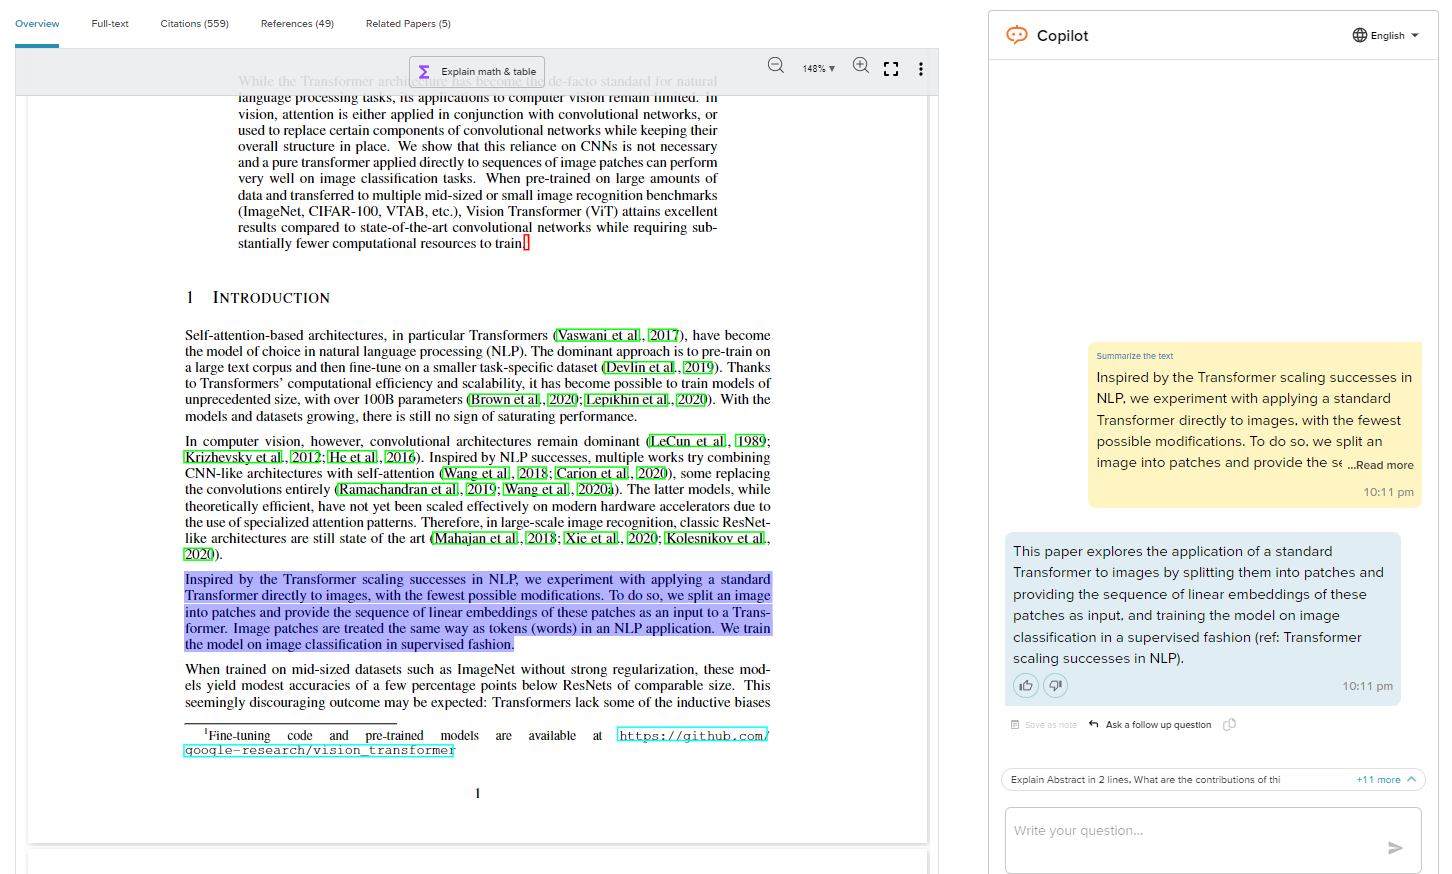
\includegraphics{img/typeset-example.png}
	\caption{Informatie opvragen van een wetenschappelijk artikel met SciSpace}
	\label{img:scispace-example}
\end{figure}

\begin{figure}[H]
	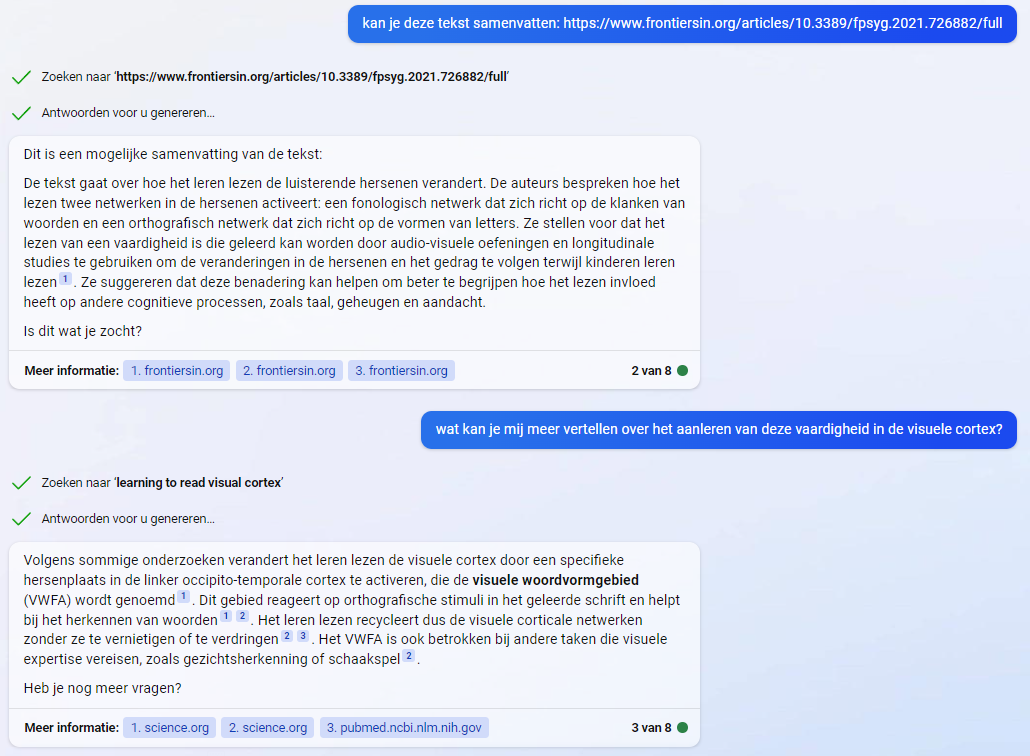
\includegraphics{img/bing-ai-chatbot-example.png}
	\caption{Tekstvereenvoudiging via de link van een wetenschappelijk artikel met Bing Chat}
	\label{img:tryout-bing-ai}
\end{figure}

\begin{figure}[H]
	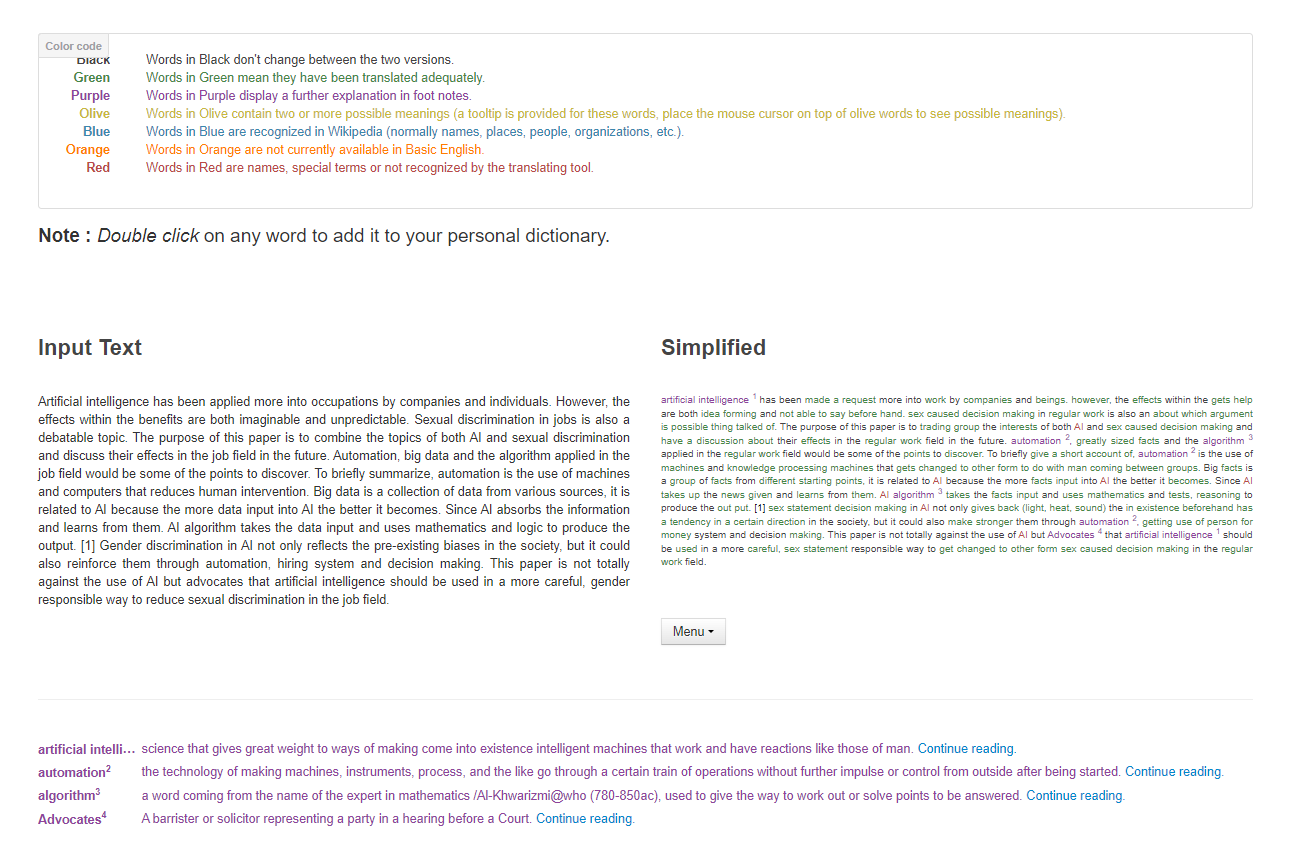
\includegraphics[width=\linewidth]{img/simplish-output.png}
	\caption{Illustratie van de tekstanalyse bij Simplish na een tekstvereenvoudiging.}
	\label{img:simplish-output}
\end{figure}

\begin{figure}[H]
	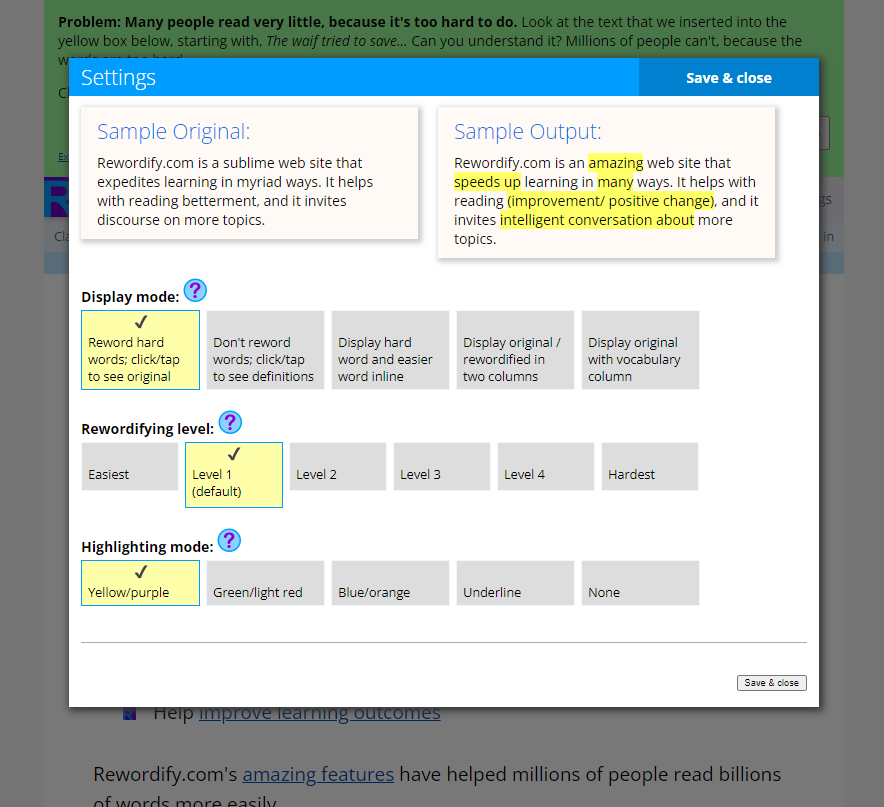
\includegraphics[width=\linewidth]{img/scholarcy-attempt.png}
	\caption{Illustratie van de tekstanalyse bij Rewordify.}
	\label{img:scholarcy}
\end{figure}
\chapter{\IfLanguageName{dutch}{Code voor tekstanalyse}{Attachment 1}}%
\label{ch:bijlage-code}

\begin{lstlisting}[language=Python, caption={Script voor fase 1 van de vergelijkende studie.}, label={code:verg-studie-phase-1}]
import os, re

def add_newline_after_dot(input_file, output_file):
	with open(input_file, 'r', encoding='utf-8') as file:
		text = file.read()
	text = re.sub(r'\d', '', text)
	modified_text = text.replace('.', '.\n')
	with open(output_file, 'w', encoding='utf-8') as file:
		file.write(modified_text)

folder_path = 'scripts\pdf'
original_scientific_papers = [f for f in os.listdir(folder_path)]

for paper in original_scientific_papers:
	input_file =  folder_path + '/' + paper
	output_file = folder_path + '/' + 'RE_' + paper
	add_newline_after_dot(input_file, output_file)
\end{lstlisting}

\newpage

\begin{center}
	\begin{lstlisting}[language=Python, caption={Script voor de tweede fase van de vergelijkende studie.}, label={code:verg-studie-phase-2}]
import os
import pandas as pd
from deep_translator import GoogleTranslator

output_csv = 'results.csv'

def translate_dutch_to_english(dutch_text_file):
	with open(dutch_text_file, 'r', encoding='utf-8') as file:
		dutch_sentences = file.readlines()
		dutch_sentences = [sentence.strip() for sentence in dutch_sentences]

	english_sentences = []
	for sentence in dutch_sentences:
		translated = GoogleTranslator(source='nl', target='en').translate(sentence)
		english_sentences.append(translated)
		df = pd.DataFrame({'Dutch': dutch_sentences, 'English': english_sentences})
		df.to_csv(str(dutch_text_file).split('.')[0] + '.csv', index=False)


	folder_path = 'scripts/pdf/'
	original_scientific_papers = [f for f in os.listdir(folder_path)]

	for paper in original_scientific_papers:
		if paper.startswith('RE_') and paper.endswith('.txt'):
			print(f'STARTING {paper}')
			dutch_text_file = folder_path + paper
			translate_dutch_to_english(dutch_text_file)
	\end{lstlisting}
\end{center}

\newpage

\begin{center}
	\begin{lstlisting}[language=Python, caption={Script voor text-analyse met Readability}, label={code:script-for-text-analysis}]
from pdfminer.high_level import extract_pages
from pdfminer.layout import LTTextContainer, LTChar
import spacy
from langdetect import detect
import pandas as pd
import os
import readability
		
		
folder_path = 'scripts\pdf'
dutch_spacy_model = "nl_core_news_md"
english_spacy_model = "en_core_web_sm"
		
dict = {nl':'nl_core_news_md',en':'en_core_web_sm'}
		
total_df = None
		
def get_sentence_length(sentence):
	doc = nlp(sentence)
	return len(doc)
		
pdf_files = [f for f in os.listdir(folder_path)]
		
for pdf in pdf_files:
	if pdf.endswith('pdf'):
		print(f'...{pdf} starting to read')
		all_pages = extract_pages(
			pdf_file='scripts\pdf/'+ pdf,
			page_numbers=[0],
			maxpages=999
		)
		
		full_text = ""
		for page_layout in all_pages:
			for element in page_layout:
				if isinstance(element, LTTextContainer):		
					for text_line in element:
						full_text += text_line.get_text()
					elif pdf.endswith('txt'):
						print(f'...{pdf} starting to read')
					with open('scripts\pdf/'+ pdf, 'r') as file:
						full_text = file.read()
		
				else:
					print(f'...{pdf} not a valid file...')
					break
		
				full_text = full_text.strip()
				full_text = full_text.replace('\n', ' ')
				lang = detect(full_text)
		
				model = dict.get(detect(full_text), dict.get('en'))
				nlp = spacy.load(model)
				doc = nlp(full_text)
		
				sentences = []
				for sentence in doc.sents:
					sentences.append(str(sentence))
		
				df = pd.DataFrame(sentences, columns=['sentence'])
				df['source'] = pdf.split('_')[0]
		
				try:
					df['title'] = pdf.split('_')[1].split('.')[0]
				except:
					df['title'] = pdf.split('_')[1]
		
				df['sentence_length'] = df['sentence'].apply(get_sentence_length)
		
				df = df[df['sentence_length'] > 4]   
		
				for key in readability.getmeasures("test")['readability grades'].keys():
					df[key] = df['sentence'].apply(lambda x: readability.getmeasures(x)['readability grades'][key])
		
				word_usage_cols = readability.getmeasures("test")['word usage'].keys()
		
				for key in word_usage_cols:
					df[key] = df['sentence'].apply(lambda x: readability.getmeasures(x, lang=lang)['word usage'][key])
		
				sentence_beginnings_cols = readability.getmeasures("test")['sentence beginnings'].keys()
				for key in sentence_beginnings_cols:
					df[key] = df['sentence'].apply(lambda x: readability.getmeasures(x, lang=lang)['sentence beginnings'][key])
		
				if total_df is None:
					total_df = df
				else:
					if not df.empty:
						total_df = pd.concat([total_df, df], ignore_index=True)
		
				total_df.to_csv(path_or_buf='text-analysis-simplification.csv', index=False)
	\end{lstlisting}
\end{center}

\chapter{\IfLanguageName{dutch}{Ontwikkeling van prototype: stappenplan}{Prototype: Development}}%
\label{ch:stappenplan-prototype}

\begin{figure}[H]
	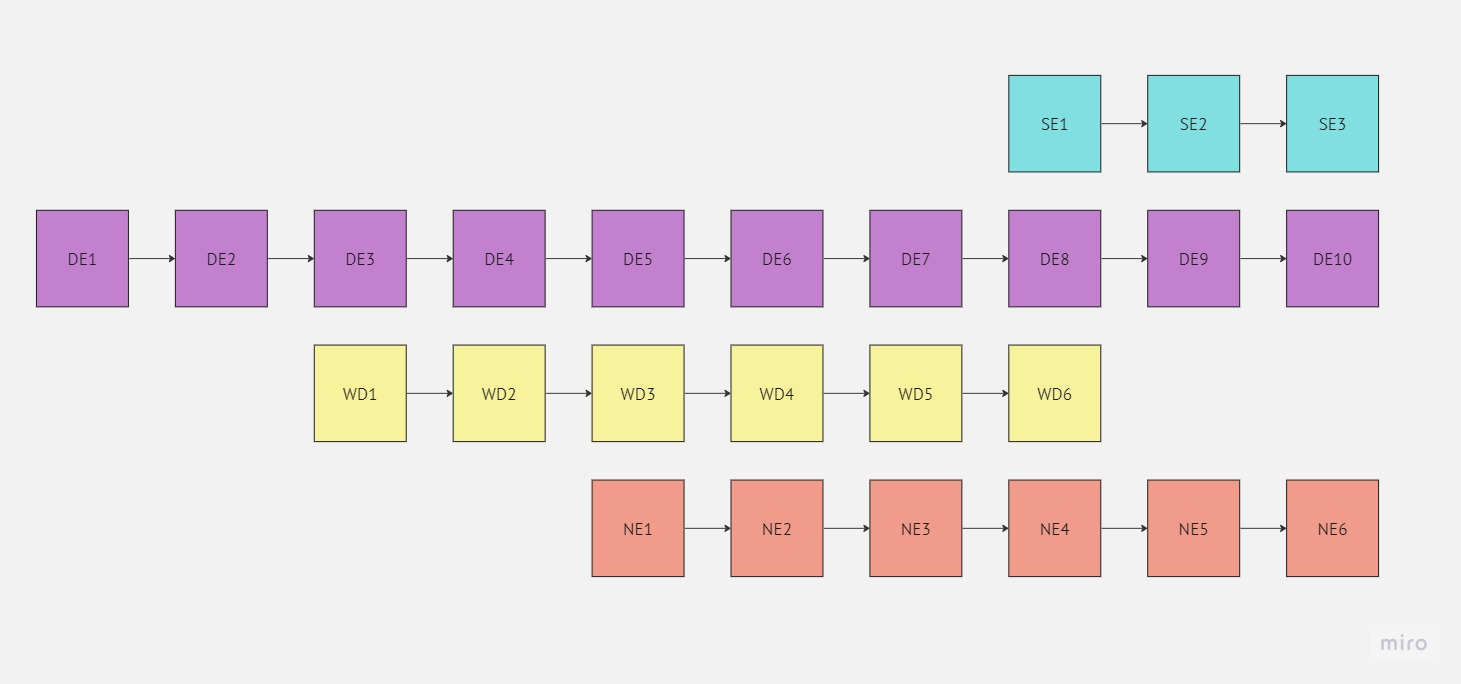
\includegraphics[width=\linewidth]{img/flowchart-development.jpg}
	\caption{Stappenplan voor de ontwikkeling van het component voor lectoren.}
	\label{img:stappenplan-leerkrachten}
\end{figure}

\begin{center}
	\begin{table}
		\begin{tabular}{ | m{2cm} | m{12cm} | } 
			\hline
			WD1 & Flask-skelet aanmaken \\
			WD2 & Formulier voor GPT-3 API-sleutel invoer maken + sessie \\
			WD3 & Formulier voor gepersonaliseerde opties van website aanmaken + sessie \\
			WD4 & Webpagina's aanmaken in HTML \& CSS \\
			WD5 & Invoerformulier maken voor PDF- en tekstupload \\
			WD6 & Invoerformulier maken voor het genereren van een gepersonaliseerde vereenvoudiging van een wetenschappelijk artikel \\
			\hline
		\end{tabular}
		\caption{Taken van de webontwikkelaar bij het uitwerken van het lerarencomponent.}
		\label{table:tasks-web-engineer}
	\end{table}
\end{center}

\begin{center}
	\begin{table}[H]
		\begin{tabular}{ | m{2cm} | m{12cm} | } 
			\hline
			NE1 & Spacy word embeddings laden \&PoS-tagging en lemmatization implementeren \\
			NE2 & Dictionary implementen voor het bijhouden van de PoS-tag per dictionary \\
			NE3 & Jupyter notebook om gepersonaliseerde prompts en aangepaste hyperparameters uit te testen voor de GPT-3 API \\
			NE4 & Jupyter notebook gebruiken om tekstvereenvoudigingsfuncties met GPT-3 API uit te testen. \\
			NE5 & Optioneel: Extra trainingsdata toevoegen aan GPT-3 model. \\
			NE6 & Code voor de voorgestelde pipeline voor ATS implementeren in Python back-end. \\
			\hline
		\end{tabular}
		\caption{Taken van de NLP Engineer bij het uitwerken van het lerarencomponent.}
		\label{table:tasks-nlp-engineer}
	\end{table}
\end{center}


\begin{center}
	\begin{table}[H]
		\begin{tabular}{|m{2cm}|m{12cm}|}
			\hline
			DE1	& Python-notebook om PDFMiner uit te testen bij willekeurige wetenschappelijke artikelen (2000 - nu) \\
			DE2 & Python-notebook opstellen om EasyOCR uit te testen bij willekeurige wetenschappelijke artikelen \\
			DE3 & Jupyter notebook om tekstdata cleaning te realiseren. De restanten van de PDF-extractie moeten weg. \\
			DE4 & Jupyter notebook om look-up methode voor synoniemen te realiseren. \\
			DE5 & Code in back-end implementeren voor PDF-upload via in-memory PDF read. \\
			DE6 & Python-notebook om Pandoc PDF \& Word-document te genereren. \\
			DE7 & Uittesten van YAML-header in Markdown-bestand voor een document op maat. \\
			DE8 & Uittesten van uitschrijven tekstinhoud naar Markdown-bestand \\
			DE9 & Implementatie code van Pandoc in Flask-framework \\
			DE10 & Code in back-end implementeren voor zippen \& doorsturen naar eindgebruiker. \\
			\hline
		\end{tabular}
		\caption{Taken van data engineer bij het uitwerken van het lerarencomponent.}
		\label{table:tasks-data-engineer}
	\end{table}
\end{center}

\begin{center}
	\begin{table}
		\begin{tabular}{|m{2cm}|m{12cm}|}
			\hline
			SE1 & Dockerfile en bijhorende requirementsfile aanmaken \\
			SE2 & Opzet in Docker realiseren \\
			SE3 & Powershell en Bash-script realiseren \\
			\hline
		\end{tabular}
		\caption{Taken van de system engineer bij het uitwerken van het lerarencomponent.}
		\label{table:tasks-system-engineer}
	\end{table}
\end{center}

\begin{figure}[H]
	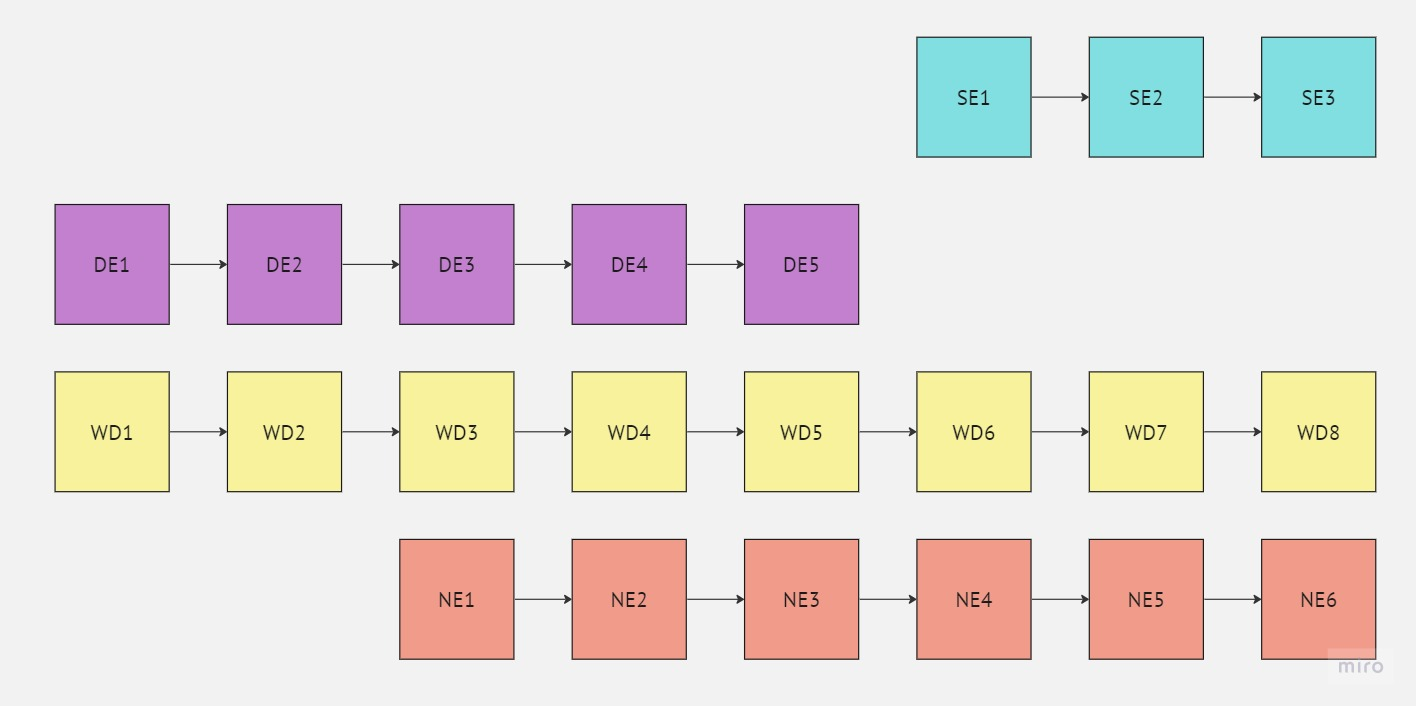
\includegraphics[width=\linewidth]{img/flowchart-development-scholars.jpg}
	\caption{Stappenplan voor de ontwikkeling van het component voor scholieren.}
	\label{img:stappenplan-scholars}
\end{figure}

\begin{center}
	\begin{table}
		\begin{tabular}{ | m{2cm} | m{12cm} | } 
			\hline
			WD1 & Flask-skelet aanmaken \\
			WD2 & Formulier voor GPT-3 API-sleutel invoer maken + sessie \\
			WD3 & Formulier voor gepersonaliseerde opties van website aanmaken + sessie \\
			WD4 & Webpagina's aanmaken in HTML \& CSS \\
			WD5 & Invoerformulier maken voor PDF- en tekstupload \\
			WD6 & JavaScript-functies schrijven voor het weergeven van grammaticale structuren, bijvoeglijke en zelfstandige naamwoorden. \\
			WD7 & JavaScript functies schrijven voor dynamische tekstaanpassing met placeholder-tekst \\
			WD8 & API-calls schrijven voor de functies: look-up, lexicale vereenvoudiging, formaatwijzigingen en ten slotte prompt-gedreven tekstvereenvoudiging \\
			\hline
		\end{tabular}
		\caption{Taken van NLP engineer bij het uitwerken van het scholierencomponent.}
		\label{table:tasks-nlp-engineer-scholars}
	\end{table}
\end{center}

\begin{center}
	\begin{table}[H]
		\begin{tabular}{|m{2cm}|m{12cm}|}
			\hline
			DE1	& Python-notebook om PDFMiner uit te testen bij willekeurige wetenschappelijke artikelen (2000 - nu) \\
			DE2 & Python-notebook opstellen om EasyOCR uit te testen bij willekeurige wetenschappelijke artikelen \\
			DE3 & Jupyter notebook om tekstdata cleaning te realiseren. De restanten van de PDF-extractie moeten weg. \\
			DE4 & Jupyter notebook om look-up methode voor synoniemen te realiseren. \\
			DE5 & Code in back-end implementeren voor PDF-upload via in-memory PDF read. \\
			\hline
		\end{tabular}
		\caption{Taken van data engineer bij het uitwerken van het scholierencomponent.}
		\label{table:tasks-data-engineer-scholars}
	\end{table}
\end{center}
\chapter{\IfLanguageName{dutch}{Code voor het prototype}{Attachment 2}}%
\label{ch:bijlage-code-2}

\begin{lstlisting}[language=Python, caption={Koppeling tussen front-end en back-end voor het inlezen van een wetenschappelijk artikel}, label={code:inlezen-wetenschappelijk-artikel-front-end-back-end}]
def setup_scholars_teachers(request):
	settings = request.form
	if 'fullText' in request.form:
		text = request.form['fullText']
		langs = detect_langs(text)
		reader = Reader()
		dict_text = reader.get_full_text_site(text)                
	elif 'pdf' in request.files:
		if 'advanced' not in settings:
			pdf = request.files['pdf']
			pdf_data = BytesIO(pdf.read())
			all_pages = extract_pages(pdf_data,page_numbers=None,maxpages=999)
			langs = detect_langs(str(all_pages))
			reader = Reader()
			full_text = reader.get_full_text_dict(all_pages)
			dict_text = reader.get_full_text_site(full_text)
		else:
			pdf = request.files['pdf']
			pdf_data = pdf.read()
			pages = convert_from_bytes(pdf_data)
			reader = Reader()
			img_text = reader.get_full_text_from_image(pages)
			langs = detect_langs(img_text)
			dict_text = reader.get_full_text_site(img_text)                            
			return dict_text, langs, 'voorbeeldtitel', 'voorbeeldonderwerp'
			
@app.route('/for-scholars', methods=['GET','POST'])
def teaching_tool():
	try:
		dict_text, langs, title, subject = setup_scholars_teachers(request)
		return render_template('for-scholars.html', pdf=dict_text, lang=langs, title=title, subject=subject)
	except Exception as e:
		return render_template('error.html',error=str(e))

@app.route('/for-teachers', methods=['GET','POST'])
def analysing_choosing_for_teachers():
	try:
		dict_text, langs, title, subject = setup_scholars_teachers(request)
		return render_template('for-teachers.html', pdf=dict_text, lang=langs, title=title, subject=subject)
	except Exception as e:
		return render_template('error.html',error=str(e))
\end{lstlisting}

\newpage

\begin{lstlisting}[language=Python, caption={Een PDF inlezen met PDFMiner}, label={code:inlezen-van-pdf}]
def get_full_text_from_pdf(self, all_pages):
	total = ""
	for page_layout in all_pages:
		for element in page_layout:
			if isinstance(element, LTTextContainer):
				for text_line in element:
					total += text_line.get_text()
	return total
\end{lstlisting}

\begin{lstlisting}[language=Python, caption={Een PDF inlezen met OCR}, label={code:reader-ocr}]
	def get_full_text_from_image(self, all_pages):
		img_files = []
		num_pages = 0
		for i, page in enumerate(all_pages):
			file = f'page_{num_pages}.jpg'
			page.save(file, 'JPEG')
			img_files.append(file)
			num_pages += 1
		
		full_text = []
		reader = easyocr.Reader(['nl'])
		for f in img_files:
			result = reader.readtext(f, detail=0)
			full_text.append(" ".join(result))
			os.remove(f)
		return " ".join(full_text)
\end{lstlisting}

\newpage

\begin{lstlisting}[language=Python, caption={Het formatteren van de tekst naar een formaat voor de website.}, label={code:reader-formatting}]
	def get_full_text_site(self, full_text):
		try:
			lang = detect(full_text)
		except:
			lang = 'en'
	
		if lang in dict:
			nlp = spacy.load(dict.get(lang))
		else:
			nlp = spacy.load(dict.get('en'))
	
		full_text = str(full_text).replace('\n', ' ')
	
		doc = nlp(full_text)
		sentences = []
		for sentence in doc.sents:
			sentences.append(sentence)
	
		pad_size = SENTENCES_PER_PARAGRAPH - (len(sentences) % SENTENCES_PER_PARAGRAPH)
		padded_a = np.pad(sentences, (0, pad_size), mode='empty')
		paragraphs = padded_a.reshape(-1, SENTENCES_PER_PARAGRAPH)
	
		text_w_pos = []
		for paragraph in paragraphs:
			paragraph_w_pos = []
		try:
			for sentence in paragraph:
			dict_sentence = {}
			for token in sentence:
				dict_sentence[token.text] = str(token.pos_).lower()
				paragraph_w_pos.append(dict_sentence)    
				text_w_pos.append(paragraph_w_pos)
		except:
			pass
			
		return text_w_pos
\end{lstlisting}

\newpage

\begin{lstlisting}[language=Python, caption={HuggingFace-klasse}, label={code:huggingface-klasse}]
class HuggingFaceModels:
	def __init__(self, key=None):
		global huggingface_api_key
		try:
			huggingface_api_key = key
		except:
			huggingface_api_key = 'not_submitted'
	
	""""""
	def query(self, payload, API_URL):
		headers = {"Authorization": f"Bearer {huggingface_api_key}"}
		response = requests.post(API_URL, headers=headers, json=payload)
		return response.json()
	
	""""""
	def scientific_simplify(self, text, lm_key):
		length = len(text)
		API_URL = huggingfacemodels.get(lm_key)
		gt = Translator()
		translated_text = gt.translate(text=text,src='nl',dest='en').text
		result = self.query({"inputs": str(translated_text),"parameters": {"max_length": length},"options":{"wait_for_model":True}}, API_URL)[0]['generated_text']
		result = gt.translate(text=result,src='en',dest='nl').text
		return result
	
	def summarize(self, text, lm_key):
		gt = Translator()        
		soup = BeautifulSoup(text, 'html.parser')
		tags = soup.find_all(True)
		split_text = {}
		for tag in tags:
			if tag.name == 'h3':
				current_key = tag.text
			if tag.name == 'p':
				split_text[current_key] = tag.text
	
		for key in split_text.keys():
			split_text[key] = str(split_text[key]).strip('\n').replace('\n', ' ').replace('\\','')
	
		result_dict = {}
		for key in split_text.keys():
			text = split_text[key]
			origin_lang = detect(text)
			nlp = spacy.load(languages.get(origin_lang, 'en'))
			doc = nlp(text)
	
		sentences = []
		for s in doc.sents:
			try:
				text = gt.translate(text=str(s), dest='en').text
				sentences.append(text)
			except Exception as e:
				print(e)
	
		API_URL = huggingfacemodels.get(lm_key)
		sentences = np.array(sentences)
		pad_size = 3 - (sentences.size % 3)
		padded_a = np.pad(sentences, (0, pad_size), mode='empty')
		paragraphs = padded_a.reshape(-1, 3)
	
		output = []
		text = ""
		for i in paragraphs:
			length = len(str(i))
			result = self.query({"inputs": str(i),"parameters": {"max_length": length},"options":{"wait_for_model":True}}, API_URL)
	
		try:
			if 'generated_text' in result[0]:
				text = result[0].get('generated_text')
	
			if 'summary_text' in result[0]:
				text = result[0].get('summary_text')
		except Exception as e:
			print(e)
	
		lang = detect(text)
		try:
			text = gt.translate(text=str(text),src=lang, dest='nl').text 
		except Exception as e:
			print(str(e))
		
		output.append(text)
		result_dict[key] = output
		return(result_dict)            
	
	"""@returns a translated sentence"""
	def translate_sentence(self, sentence):
		translator  = Translator()
		result = translator.translate(
			text=sentence,
			dest='nl'
		)
		return result.text
\end{lstlisting}

\begin{lstlisting}[language=Python, caption={De gebruikte Python-klasse voor gepersonaliseerde ATS}, label={listing:gpt-class}]
class GPT():
	""" @sets openai.api_key """
	def __init__(self, key=None):
		global gpt_api_key
		if key is None:
			gpt_api_key = 'not-submitted'
			openai.api_key = key
		else:
			gpt_api_key = key
			openai.api_key = key
	
	""" @returns prompt, result from gpt """
	def look_up_word_gpt(self, word, context):
		try:
			prompt = f"""
		Give a simple Dutch explanation in one sentence for this word in the given context. Give the PoS-tag and Dutch definition: '{word}'
		context: {context}
		format: PoS-tag | definition
		///
	"""
	
			result = openai.Completion.create(
				prompt=prompt,
				temperature=0,
				max_tokens=50,
				model=COMPLETIONS_MODEL,
				top_p=0.9,
				stream=False
			)["choices"][0]["text"].strip(" \n")    
			return result, word, prompt	
		except Exception as e:
			return 'error', str(e), str(e)
	
	""" @returns prompt, result from gpt """
	def give_synonym(self, word, context):
		try:
			prompt = f"""
			Give a Dutch synonym for '{word}'. If there is no Dutch synonym available, explain it between curly brackets.
			context:
			{context}
			"""
			
			result = openai.Completion.create(
				prompt=prompt,
				temperature=0,
				max_tokens=10,
				model=COMPLETIONS_MODEL,
				top_p=0.9,
				stream=False
				)["choices"][0]["text"].strip(" \n")    
			return result, word, prompt
		except Exception as e:
			return 'Open AI outage of problemen', str(e)
		
	def personalised_simplify(self, sentence, personalisation):
	if 'summary' in personalisation:
		prompt = f"""
		Simplify the sentences in the given text and {", ".join(personalisation)}
		:return: A list of simplified sentences divided by a '|' sign
		///
		{sentence}
		"""
	else:
		prompt = f"""
		Explain this in own Dutch words and {", ".join(personalisation)}
		///
		{sentence}
		"""
	
	try:
		result = openai.Completion.create(
			prompt=prompt,
			temperature=0,
			max_tokens=len(prompt),
			model=COMPLETIONS_MODEL,
			top_p=0.9,
			stream=False
		)["choices"][0]["text"].strip(" \n")
	
		if 'summary' in personalisation:
			result = result.split('|')
		else:
			result = [result]
		
		return result, prompt
	except Exception as e:
		return str(e), prompt 
	
	def personalised_simplify_w_prompt(self, sentences, personalisation):
		try:
			result = openai.Completion.create(
				prompt=personalisation,
				temperature=0,
				max_tokens=len(personalisation)+len(sentences),
				model=COMPLETIONS_MODEL,
				top_p=0.9,
				stream=False
			)["choices"][0]["text"].strip(" \n")
			return result, personalisation
		except Exception as e:
			return str(e), personalisation
		
	
	def summarize(self, full_text_dict, personalisation):
		soup = BeautifulSoup(full_text_dict, 'html.parser')
		tags = soup.find_all(True)
		split_text = {}
	
	for tag in tags:
		if tag.name == 'h3':
			current_key = tag.text
	
		if tag.name == 'p':
			split_text[current_key] = tag.text
		
		for key in split_text.keys():
			split_text[key] = str(split_text[key]).strip('\n')\
					.strip('\\').replace('\\','')
	
		new_text = {}
		for title in split_text.keys():
			text = split_text[title]
		if len(text) > 1000:
			index = len(text) // 2
			text_to_prompt = [text[:index], text[index:] ]
		else:
			text_to_prompt = [text]
	
		full_chunk_result = ""
		for chunk in text_to_prompt:	
			if 'summation' not in personalisation:
			prompt = f"""
			Rewrite this with {", ".join(personalisation)}
			///
			{chunk}
			"""
			else:
			prompt = f"""
			Rewrite this as a list of simplified Dutch sentences with {", ".join(personalisation)}
			:return: A list of simplified sentences divided by a '|' sign
			///
			{chunk}
			"""
	
			full_chunk_result += str(openai.Completion.create(prompt=prompt,temperature=0,max_tokens=500,model=COMPLETIONS_MODEL,top_p=0.9,stream=False)["choices"][0]["text"].strip(" \n"))
		new_text[title] = [full_chunk_result]
		return new_text
\end{lstlisting}

\begin{lstlisting}[language=Python, caption={Writer-klasse omvattende de code om dynamische PDF- en Word-documenten te genereren.}, label={code:writer-klasse}]
import subprocess, io, os, pypandoc
from datetime import date
import zipfile

markdown_file = "saved_files/file.md"
zip_filename = 'saved_files/simplified_docs.zip'
pdf_file = "saved_files/output.pdf"
docx_file = "saved_files/output.docx"
DATE_NOW = str(date.today())

class Creator():
	def create_header(self, title, margin, fontsize, chosen_font, chosen_title_font, word_spacing, type_spacing):
		with open(markdown_file, 'w', encoding='utf-8') as f:
			f.write("---\n")
			f.write(f"title: {title}\n") 
			f.write(f"mainfont: {chosen_font}.ttf\n")
			f.write(f"titlefont: {chosen_title_font}.ttf\n")
			f.write(f'date: {DATE_NOW}\n')
			f.write(f'document: article\n')
			f.write(f'geometry: margin={margin}cm\n')
			f.write(f'fontsize: {fontsize}pt\n')
			f.write('header-includes:\n')
			f.write(f'- \spaceskip={word_spacing}cm\n')
			f.write(f'- \\usepackage{{setspace}}\n')
			f.write(f'- \{type_spacing}\n')
			f.write("---\n")
	
	
	def generate\_glossary(self, list):
		with open(markdown_file, 'a', encoding='utf-8') as f:
			f.write("---\n")
			f.write("# Woordenlijst\n")
			f.write("| Woord | Soort | Definitie |\n")
			f.write("| --- | --- | --- |\n")
			for word in list.keys(): 
				f.write(f"| {word} | {list[word]['type']} | {list[word]['definition']} |\n")
	
	""""""
	def generate_summary(self, full_text):
		with open(markdown_file,'a', encoding="utf-8", errors="surrogateescape") as f:
			for key in full_text.keys():
				title = str(key).replace('\n',' ')
				text = full_text[key]
				f.write('\n\n')
				f.write(f'## {title}')
				f.write('\n\n')
				f.write(" ".join(text))
				f.write('\n\n')
	
	
	def generate_summary_w_summation(self, full_text):
		with open(markdown_file,'a', encoding="utf-8", errors="surrogateescape") as f:
			for key in full_text.keys():
				title = str(key).replace('\n',' ')
				text = full_text[key][0].split('|')
				f.write('\n\n')
				f.write(f'## {title}')
				for sentence in text:    
				f.write('\n\n')
				f.write(f'* {sentence}')
				f.write('\n\n')
	
	
	def create_pdf(self, title, margin, list, full_text, fonts, word_spacing, type_spacing, summation):
		if title is not None:
			self.create_header(title=title, margin=margin, fontsize=14, chosen_font=fonts[0], chosen_title_font=fonts[1], word_spacing=word_spacing, type_spacing=type_spacing)
		else:
			self.create_header(title='Vereenvoudigde tekst', margin=0.5, fontsize=14, chosen_font=fonts[0], chosen_title_font=fonts[1], word_spacing=word_spacing, type_spacing=type_spacing)
	
		"""GLOSSARY"""
		if len(list) != 0:
			self.generate_glossary(list=list)
		
		"""SUMMARY"""
		if summation:
			self.generate_summary_w_summation(full_text=full_text)
		else:
			self.generate_summary(full_text=full_text)
	
		"""FILE_CREATION"""
		pypandoc.convert_file(source_file=markdown_file, to='docx', outputfile=docx_file,   extra_args=["-M2GB", "+RTS", "-K64m", "-RTS"])
		pypandoc.convert_file(source_file=markdown_file, to='pdf',  outputfile=pdf_file,    extra_args=['--pdf-engine=xelatex'])
		with zipfile.ZipFile(zip_filename, 'w') as myzip:
		myzip.write(pdf_file)
		myzip.write(docx_file)
\end{lstlisting}

\begin{lstlisting}[language=JavaScript, caption={De toegepaste scripts voor het verwijderen van adjectieven en togglen van type woorden.}, label={code:js-toggle-adjectives-nouns-verbs}]
/* Adjectieven uitfilteren op basis van span-tag */
function removeAdjectives() {
	const elements = document.querySelectorAll(".adj");
	elements.forEach(function (element) {
		element.remove();
	});
}

/* Checkboxes */
const nouns = document.getElementById('noun-show');
const verbs = document.getElementById('verb-show');
const adjs = document.getElementById('adj-show');

nouns.addEventListener('change', function () {
	if (this.checked) {
		const color = document.getElementById('colorForNouns').value;
		console.log(color);
		const elements = document.querySelectorAll("span.noun");
		elements.forEach(function (element) {
			element.style.color = color;
		});
	} else {
		const elements = document.querySelectorAll("span.noun");
		elements.forEach(function (element) {
			element.style.color = "black";
		});
	}
});

verbs.addEventListener('change', function () {
	if (this.checked) {
		const color = document.getElementById('colorForVerbs').value;
		const elements = document.querySelectorAll("span.verb, span.aux");
		console.log(color, elements[0])
		elements.forEach(function (element) {
			element.style.color = color;
		});
	} else {
		const elements = document.querySelectorAll("span.verb, span.aux");
		elements.forEach(function (element) {
			element.style.color = "black";
		});
	}
});


adjs.addEventListener('change', function () {
	if (this.checked) {
		const color = document.getElementById('colorForAdjs').value;
		const elements = document.querySelectorAll("span.adj");
		elements.forEach(function (element) {
			element.style.color = color;
		});
	} else {
		const elements = document.querySelectorAll("span.adj");
		elements.forEach(function (element) {
			element.style.color = "black";
		});
	}
});
\end{lstlisting}

\begin{lstlisting}[language=JavaScript, caption={De toegepaste scripts voor enkel het scholierencomponent.}, label={code:js-scholars}]
document.addEventListener("DOMContentLoaded", () => {
	const spans = document.querySelectorAll(".verb, .adj, .noun, .aux");
	spans.forEach((span) => {
		span.addEventListener("click", async (event) => {
			const radioButton = document.querySelector("#explainWords");
			if (radioButton && !radioButton.checked) {
				return;
			}
			let leftSideTag = span.closest("p");
			let rightSideTag = leftSideTag.nextElementSibling;
			sentence_of_origin = span.closest(".sentence");
			
			var context = "";
			for (const child of sentence_of_origin.children) {
				context = context + " " + child.textContent;
			}
			const word = event.target.textContent;
			const response = await fetch(`http://localhost:5000/look-up-word`, {
				method: "POST",
				headers: { "Content-Type": "application/json" },
				body: JSON.stringify({ word: word, sentence: context }),
			});
			result = await response.json();
			
			if (result.result == "error") {
				alert("Incorrect API key provided: " + result.word);
			} else {
				var pos_tag = result.result.split('|')[0];
				var definition = result.result.split('|')[1];
				let table = document.querySelector(".table-glossary");
				let newRow = table.insertRow(-1);
				let cell1 = newRow.insertCell(0);
				let cell2 = newRow.insertCell(1);
				let cell3 = newRow.insertCell(2);
				cell1.innerHTML = result.word;
				cell2.innerHTML = 'Bijvoeglijk naamwoord';
				cell3.innerHTML = definition.lower;
			}
		});
	});
});

/* --- */
async function syntacticSimplification() {
	var selectedText = window.getSelection().toString();
	if (selectedText == "" || selectedText == null) {
		alert('Markeer de tekst die u wilt vereenvoudigen.');
		return;
	}
	
	var dazzle = document.querySelector(".dazzle");
	var p = document.createElement("p");
	var p2 = document.createElement("p");
	var text = document.createTextNode("Zinsbouw vereenvoudigen...");
	var prompt = document.createTextNode("...");
	p.appendChild(prompt);
	dazzle.appendChild(p);
	p2.appendChild(text);
	dazzle.appendChild(p2);
	const response = await fetch(`http://localhost:5000/simplify`, {
		method: "POST",
		headers: { "Content-Type": "application/json" },
		body: JSON.stringify({ text: selectedText, key: "sc" }),
	});
	result = await response.json();
	prompt.nodeValue = JSON.stringify(result.prompt);
	text.nodeValue = JSON.stringify(result.result);
}

/* --- */
function insertAfter(newNode, existingNode) {
	existingNode.parentNode.insertBefore(newNode, existingNode.nextSibling);
}

/* --- */
document.addEventListener("DOMContentLoaded", () => {
	const spans = document.querySelectorAll(".sentence");
	spans.forEach((span) => {
		span.addEventListener("click", async (event) => {
			const radioButton = document.querySelector("#simplifySentences"); // get reference to radio button
			if (radioButton && !radioButton.checked) {
				return;
			}
			sentence_of_origin = span.closest(".sentence");
			var context = "";
			for (const child of sentence_of_origin.children) {
				context = context + " " + child.textContent;
			}
			const response = await fetch(`http://localhost:5000/simplify`, {
				method: "POST",
				headers: { "Content-Type": "application/json" },
				body: JSON.stringify({ text: context, key: "sc" }),
			});
			result = await response.json();
			var p = document.createElement("p");
			newNode = document.createTextNode(JSON.stringify(result.result));
			p.append(newNode);
			insertAfter(p, span);
			sentence_of_origin.innerHTML = "<del>" + context + "</del>";
			parent = sentence_of_origin.parent;
		});
	});
});

async function personalizedSimplification() {
	var selectedText = window.getSelection().toString();
	if (selectedText == "" || selectedText == null) {
		alert('Markeer de tekst die u wilt vereenvoudigen.');
		return;
	}
	
	let checkedValues = [];
	let checkboxes = document.querySelectorAll(
	'.personalisation input[type="checkbox"]'
	);
	
	checkboxes.forEach((checkbox) => {
		if (checkbox.checked) {
			checkedValues.push(checkbox.name);
		}
	});
	
	if (checkedValues.length == 0) {
		alert('Duidt één van de onderstaande opties aan.');
		return;
	}
	
	var selectedChoices = checkedValues;
	var prompt = document.createTextNode("Gepersonaliseerde tekst ophalen...");
	var text = document.createTextNode("...");
	var dazzle = document.querySelector(".dazzle");
	var p = document.createElement("p");
	var p2 = document.createElement("p");
	
	p.appendChild(prompt);
	dazzle.appendChild(p);
	p2.appendChild(text);
	dazzle.appendChild(p2);
	
	const response = await fetch(`http://localhost:5000/personalized-simplify`, {
		method: "POST",
		headers: { "Content-Type": "application/json" },
		body: JSON.stringify({ text: selectedText, choices: selectedChoices }),
	});
	
	result = await response.json();
	
	array = result.result;
	console.log(array);
	
	if (array.length > 1) {
		prompt.nodeValue = JSON.stringify(result.prompt);
		const ul = document.createElement("ul");
		array.forEach((item) => {
			const li = document.createElement("li");
			li.textContent = item;
			ul.appendChild(li);
		});
		text.remove;
		p2.appendChild(ul);
	} else {
		prompt.nodeValue = JSON.stringify(result.prompt);
		text.nodeValue = JSON.stringify(result.result[0]);
	}
}

async function askGPT() {
	var selectedText = window.getSelection().toString();
	if (selectedText == "" || selectedText == null) {
		alert('Markeer de tekst die u wilt vereenvoudigen.');
		return;
	}
	
	var promptText = window.prompt(
	"Wat wilt u doen met de geselecteerde tekst? Schrijf hier de prompt...'"
	);
	
	var fullPrompt = promptText + "///\n" + selectedText;
	var prompt = document.createTextNode("Gepersonaliseerde tekst ophalen...");
	var text = document.createTextNode("");
	var dazzle = document.querySelector(".dazzle");
	var p = document.createElement("p");
	var p2 = document.createElement("p");
	
	p.appendChild(prompt);
	dazzle.appendChild(p);
	p2.appendChild(text);
	dazzle.appendChild(p2);
	
	const response = await fetch(
	`http://localhost:5000/personalized-simplify-custom-prompt`,
	{
		method: "POST",
		headers: { "Content-Type": "application/json" },
		body: JSON.stringify({ text: selectedText, prompt: fullPrompt }),
	}
	);
	
	result = await response.json();
	console.log(result);
	prompt.nodeValue = JSON.stringify(result.prompt);
	text.nodeValue = JSON.stringify(result.result);
}

async function emptyChat() {
	const dazzleDiv = document.querySelector(".dazzle");
	dazzleDiv.innerHTML = "";
}

window.onload = async function () {
	/* --- */
	var url = `http://localhost:5000/get-settings-user`;
	const response = await fetch(url, { method: "POST" });
	var result = await response.json();
	document.body.style.fontSize = result.fontSize + "px";
	document.body.style.fontFamily = result.fontSettings;
	document.body.style.backgroundColor = result.favcolor;
	document.body.style.lineHeight = result.lineHeight + "cm";
	document.body.style.wordSpacing = result.wordSpacing + "cm";
	document.body.style.textAlign = result.textAlign;
	
	/* --- */
	var url = "http://localhost:5000/get-session-keys";
	const session_keys_response = await fetch(url, { method: "POST" });
	result = await session_keys_response.json();
	
	let missing_keys = [];
	
	if (result.hf_api_key === undefined) {
		missing_keys.push("HuggingFace");
		document.querySelector("#simple-syntactic-simplification").style.display =
		"none";
	}
	
	if (result.gpt3 === undefined) {
		missing_keys.push("GPT-3");
		document.querySelector("#prompt-synt-simplification").style.display =
		"none";
		document.querySelector("#personalized-synt-simplification").style.display =
		"none";
		document.querySelector(".personalisation").style.display = "none";
	}
	
	if (missing_keys.length > 0){
		alert("Sleutel(s) voor " + missing_keys.join(" & ") + " ontbreken.");
	}
};

\end{lstlisting}

\begin{lstlisting}[language=JavaScript, caption={De toegepaste scripts voor enkel het lerarencomponent.}, label={code:js-teachers}]
/* --- */
const checkbox = document.querySelector("#personalizedSummary");
const fieldsets = document.querySelectorAll(".personalized");
checkbox.addEventListener("change", () => {
	fieldsets.forEach((fieldset) => {
		if (checkbox && checkbox.checked) {
			fieldset.style.display = "block";
		} else {
			fieldset.style.display = "none";
		}
	});
});

/* Add word to glossary */
var checkboxAddWordToGlossary = document.getElementById(
"checkboxAddWordToGlossary"
);
checkboxAddWordToGlossary.addEventListener("change", function () {
	if (checkboxAddWordToGlossary && checkboxAddWordToGlossary.checked) {
		const words = document.querySelectorAll(
		"span.verb, span.noun, span.aux, span.verb, span.adj"
		);
		words.forEach((w) => {
			w.addEventListener("click", async (event) => {
				if (checkboxAddWordToGlossary.checked) {
					var pTag = event.target;
					sentence_of_origin = w.closest("span.sentence");
					var context = "";
					for (const child of sentence_of_origin.children) {
						context = context + " " + child.textContent;
					}
					console.log(context);
					var textarea = document.getElementById("glossaryList");
					pTag.style.backgroundColor = "black";
					pTag.style.color = "white";
					pTag.style.fontWeight = "bold";
					textarea.value += pTag.innerHTML + ":" + context + "\n";
					console.log(textarea.value);
				}
			});
		});
	}
});

/* Deleting sentences */
const checkboxDeleteSents = document.getElementById("checkboxDeleteSents");
checkboxDeleteSents.addEventListener("change", function () {
	if (checkboxDeleteSents && checkboxDeleteSents.checked) {
		const sentences = document.querySelectorAll(".sentence");
		sentences.forEach((span) => {
			span.addEventListener("click", async (event) => {
				if (checkboxDeleteSents.checked) span.remove();
			});
		});
	}
});

/* Tekst toevoegen */
function addTextToTextArea() {
	const fullTextBox = document.querySelector(".left-container").innerHTML;
	var textarea = document.getElementById("fullText");
	textarea.value = fullTextBox;
	document.getElementById("summarize-with-presets-button").disabled = false;
}

function makeTitle(button) {
	const titleText = document.getElementById("title").value;
	const newTitle = document.createElement("h3");
	newTitle.innerText = titleText;
	const titleContainer = document.getElementById("title").parentElement;
	titleContainer.replaceChild(newTitle, document.getElementById("title"));
	button.parentNode.removeChild(button);
}

function deleteTitle(button) {
	var parent = button.parentNode;
	parent.parentNode.removeChild(parent);
}

window.onload = async function () {
	/* --- */
	var url = `http://localhost:5000/get-settings-user`;
	const response = await fetch(url, { method: "POST" });
	var result = await response.json();
	document.body.style.fontSize = result.fontSize + "px";
	document.body.style.fontFamily = result.fontSettings;
	document.body.style.backgroundColor = result.favcolor;
	document.body.style.lineHeight = result.lineHeight + "cm";
	document.body.style.wordSpacing = result.wordSpacing + "cm";
	document.body.style.textAlign = result.textAlign;
	
	/* --- */
	var url = "http://localhost:5000/get-session-keys";
	const session_keys_response = await fetch(url, { method: "POST" });
	result = await session_keys_response.json();
	
	let missing_keys = [];
	
	if (result.hf_api_key === undefined) {
		missing_keys.push("HuggingFace");
		document.getElementById("huggingface").innerHTML =
		"Geen HuggingFace sleutel werd opgegeven. ";
		document.getElementById("huggingface").style.color = "red";
	} else {
		document.getElementById("huggingface").innerHTML =
		"HuggingFace API-sleutel:\t" + result.hf_api_key;
	}
	
	if (result.gpt3 === undefined) {
		missing_keys.push("GPT-3");
		document.getElementById("gpt3").innerHTML =
		"Geen GPT-3 sleutel werd opgegeven.";
		document.getElementById("gpt3").style.color = "red";
	} else {
		document.getElementById("gpt3").innerHTML =
		"GPT-3 API-sleutel: " + result.gpt3;
	}
	
	if (missing_keys.length > 0) {
		alert("Sleutel(s) voor " + missing_keys.join(" & ") + " ontbreken.");
	}
};

\end{lstlisting}


\begin{lstlisting}[language=Dockerfile, caption={Dockerfile voor het prototype.}, label={code:dockerfile}]
FROM python:3.8-slim-buster

WORKDIR /app

COPY requirements.txt requirements.txt

RUN apt-get update && apt-get install -y pandoc texlive-xetex texlive poppler-utils

RUN pip3 install -r requirements.txt \
&& python3 -m spacy download nl_core_news_md \
&& python3 -m spacy download en_core_web_md

COPY . .

CMD [ "python3", "-m" , "flask", "run", "--host=0.0.0.0", "--port=5000"]
\end{lstlisting}


\begin{lstlisting}[language=Powershell, caption={Script voor het opstarten van de Docker-container voor Windows-gebruikers}, label={code:shell-boot}]
@echo off

cd web-app
docker stop text-application-prototype
docker rm text-application-prototype

docker rmi text-app

docker build -t text-app .
docker run --name text-application-prototype --network webapp_simplification -d -p 5000:5000 text-app
\end{lstlisting}

\begin{lstlisting}[language=Bash, caption={Script voor het opstarten van de Docker-container voor Unix-gebruikers}, label={code:bash-boot}]
#!/bin/sh
	
cd web-app || exit
docker stop text-application-prototype
docker rm text-application-prototype
	
docker rmi text-app
	
docker build -t text-app .
docker run --name text-application-prototype --network webapp_simplification -d -p 5000:5000 text-app
\end{lstlisting}
\chapter{\IfLanguageName{dutch}{Figuren Vergelijkende Studie}{Comparitive Study Figures}}%
\label{ch:afbeeldingen-resultaten-verg-studie}


\begin{table}[h]
	\centering
	\begin{tabular}{ | m{3cm} | m{3cm} | m{3cm} | } 
		\hline
		Bron & #Zinnen in A1 & #Zinnen in A2 \\
		\hline
		Oorspronkelijk & 78  & 159 \\ 
		\hline
		MTS (door leerkracht) & 43 & 45 \\
		\hline
		MTS (door leerling) & n.v.t. & 50 \\
		\hline
		T1 & 101 & 209 \\
		\hline
		T2 & 82 & 209 \\
		\hline
		T3 & 100 & 209 \\
		\hline
		T4 P1 & 61 & 98 \\
		\hline
		T4 P2 & 89 & 133 \\
		\hline
		T4 P3 & 39 & 55 \\
		\hline
	\end{tabular}
	\label{table:resultaten-aantal-zinnen}
	\caption{Aantal zinnen (gemeten met Spacy sentence embeddings) per tekst.}
\end{table}


\begin{figure}
	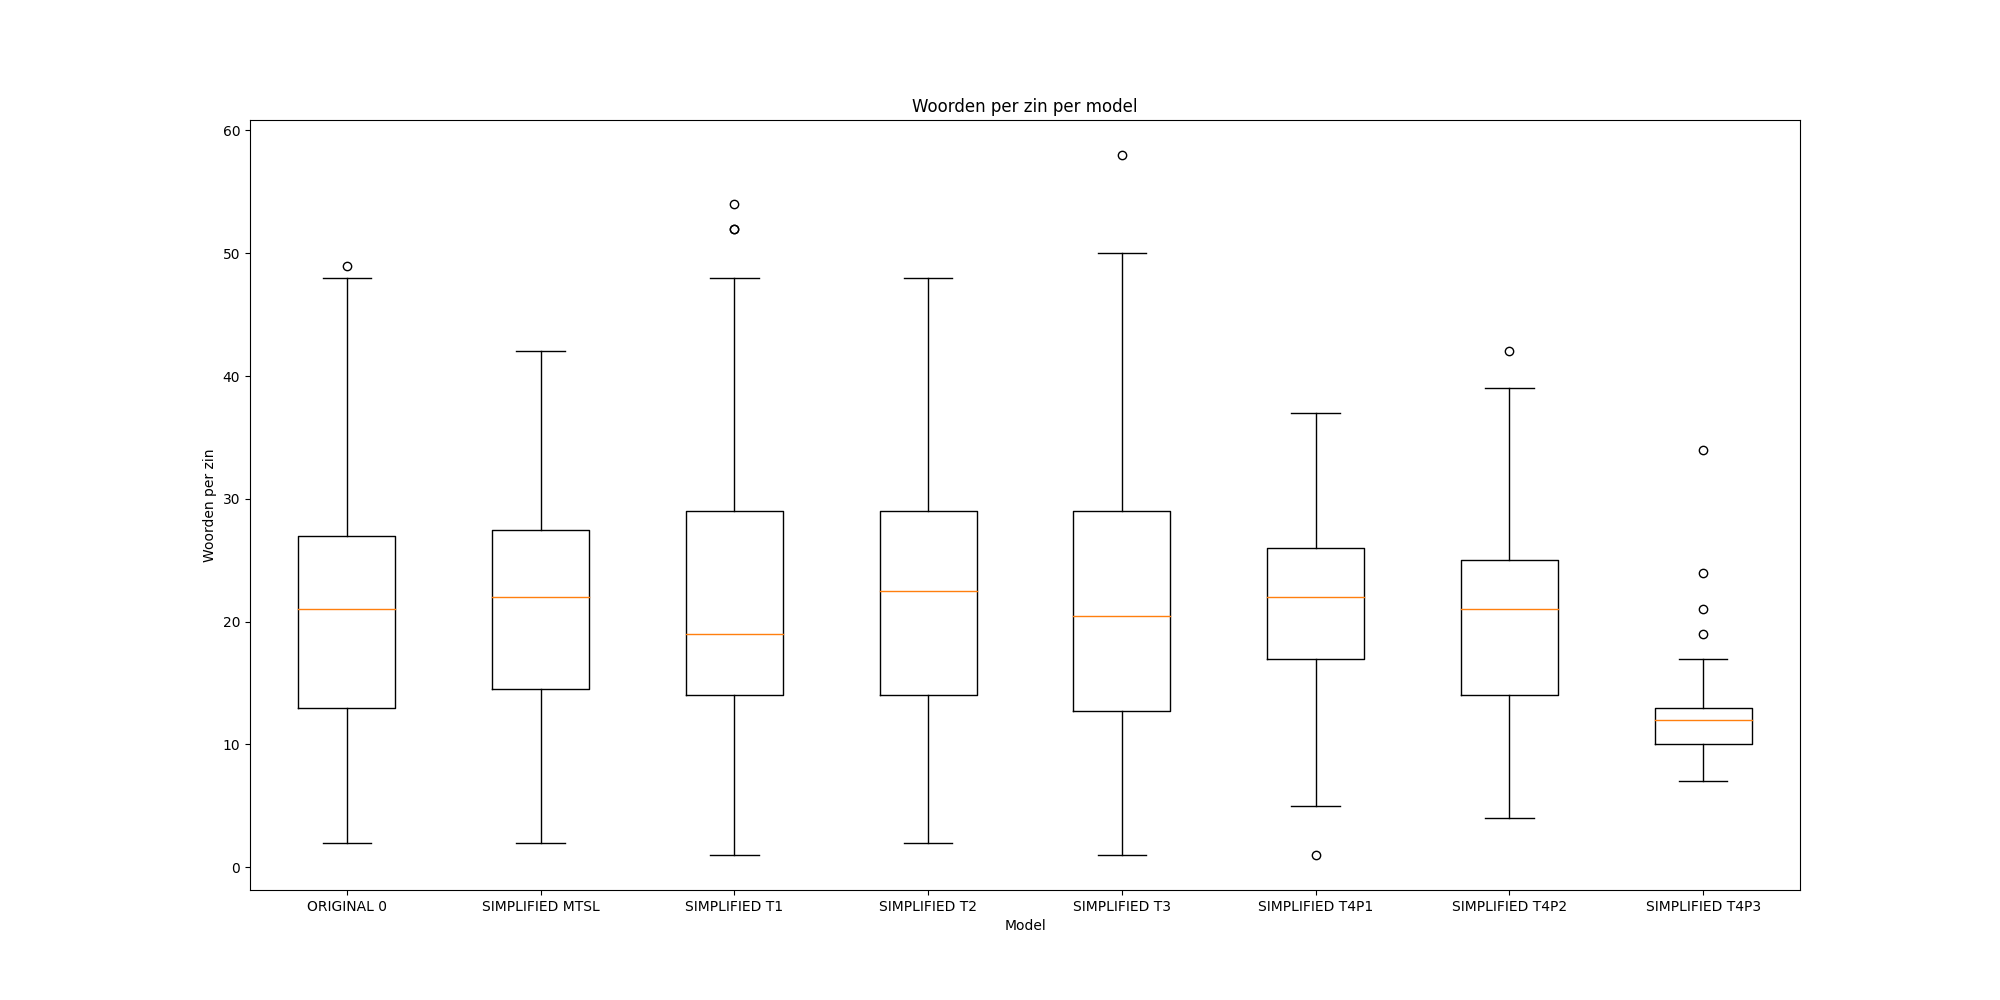
\includegraphics[width=\linewidth]{img/boxplot-avg-a1.png}
	\caption{Overzicht van het minimum, maximum en gemiddeld aantal woorden per zin per model in A1.}
	\label{img:boxplot-min-max-avg-words-a1}
\end{figure}

\begin{figure}
	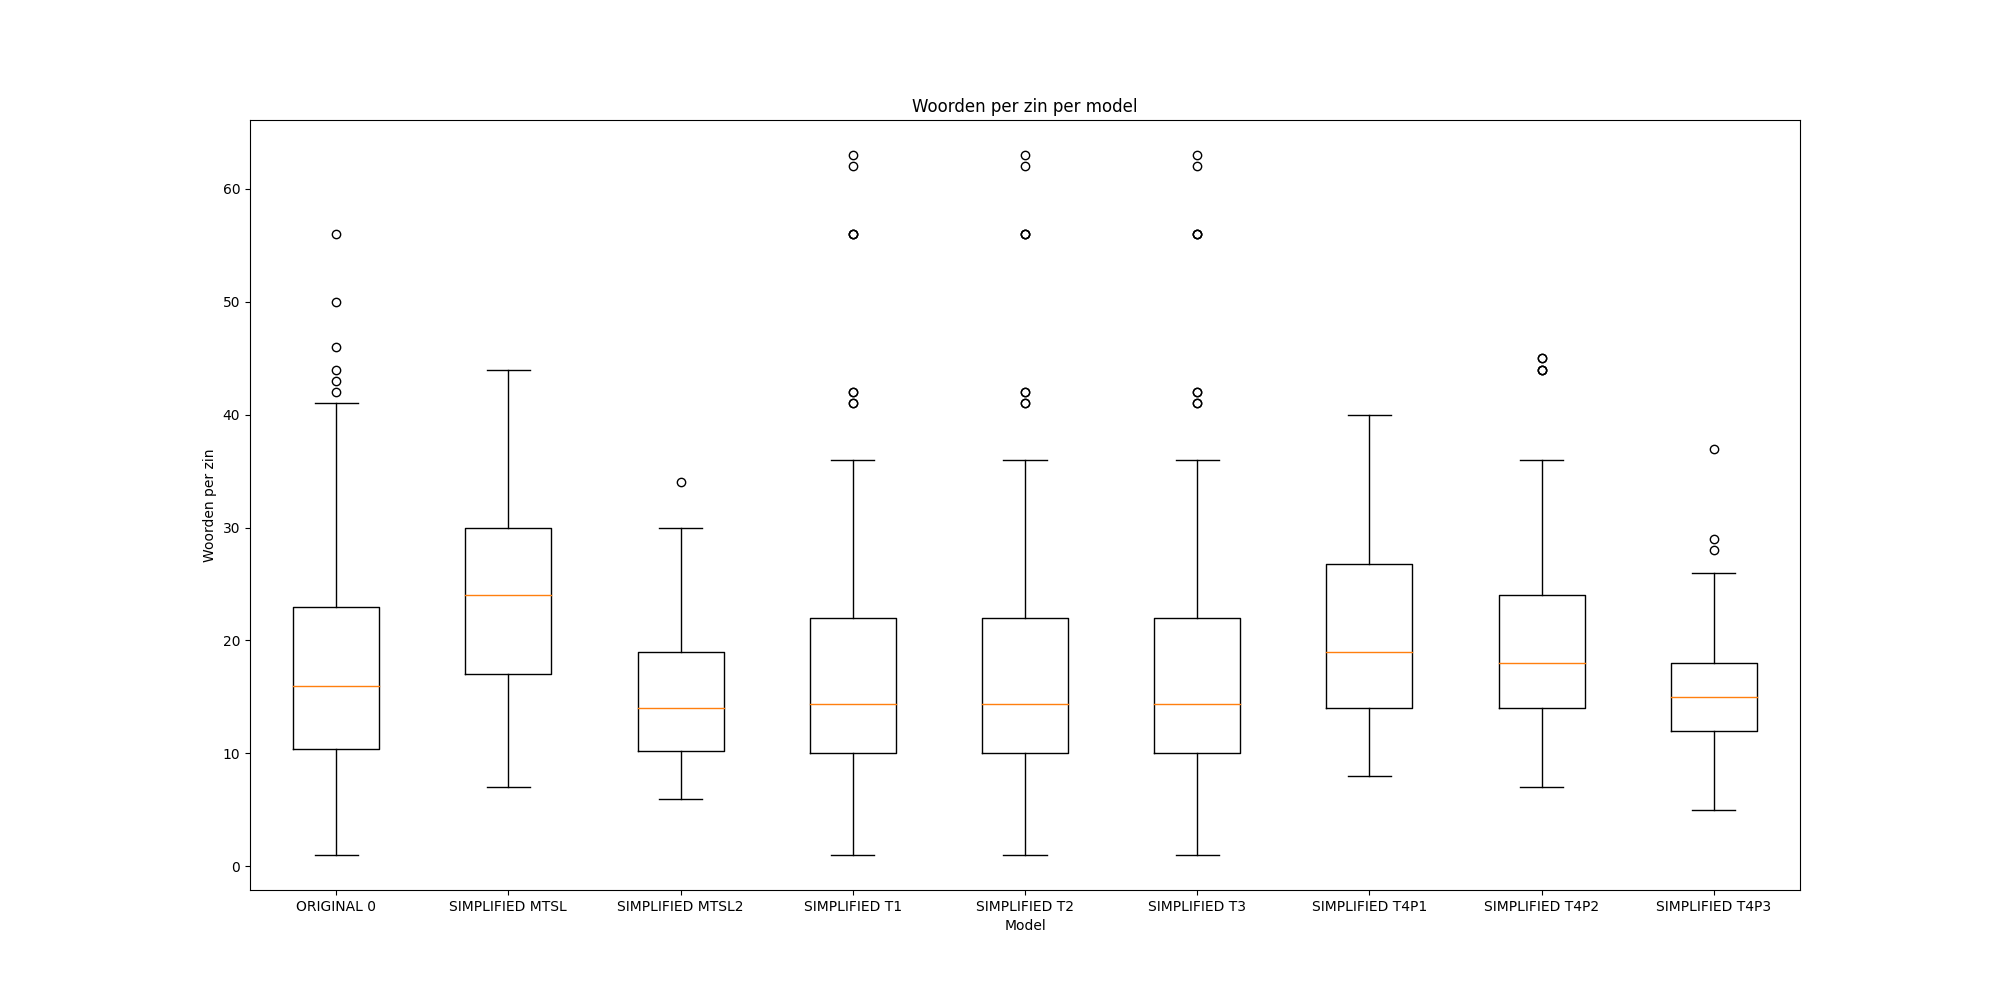
\includegraphics[width=\linewidth]{img/boxplot-avg-a2.png}
	\caption{Overzicht van het minimum, maximum en gemiddeld aantal woorden per zin per model in A2.}
	\label{img:boxplot-min-max-avg-words-a2}
\end{figure}


\begin{figure}
	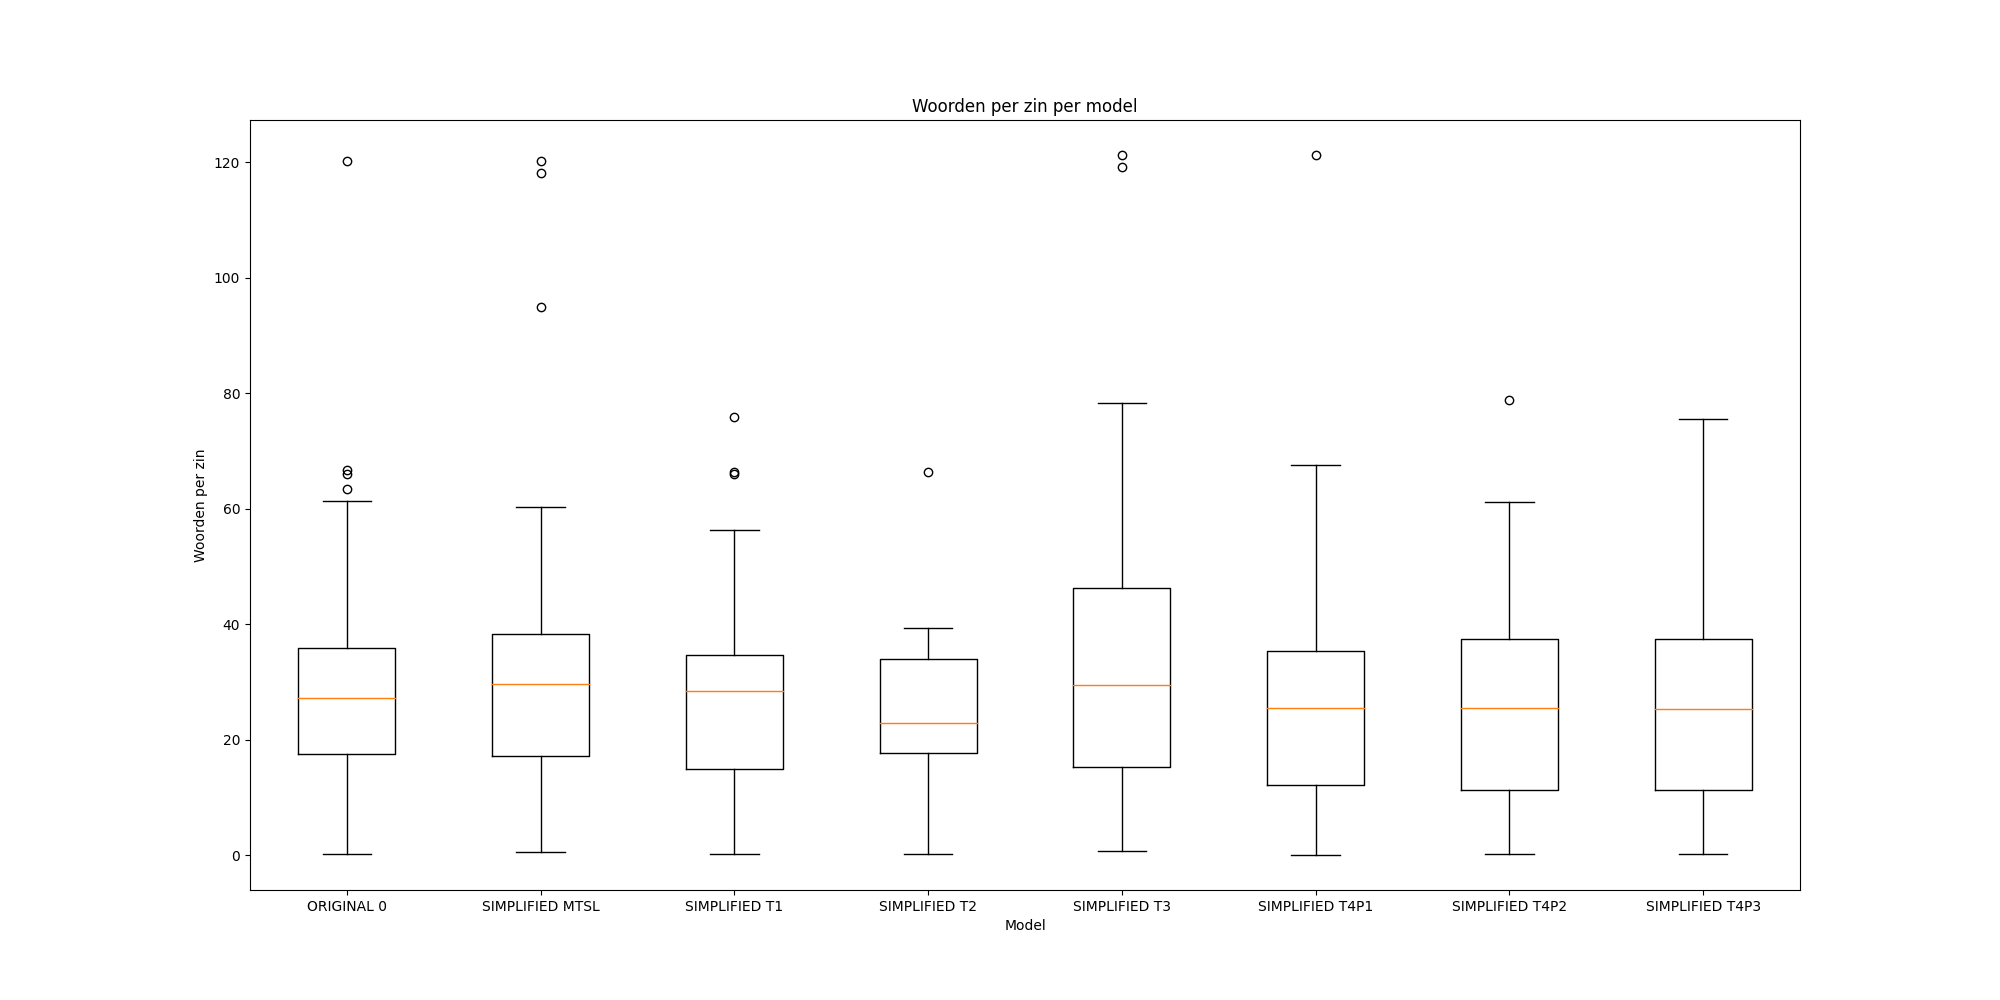
\includegraphics[width=\linewidth]{img/boxplot-fre-a1.png}
	\caption{Boxplot van de FRE-scores voor A1.}
	\label{img:boxplot-fre-a1}
\end{figure}

\begin{figure}
	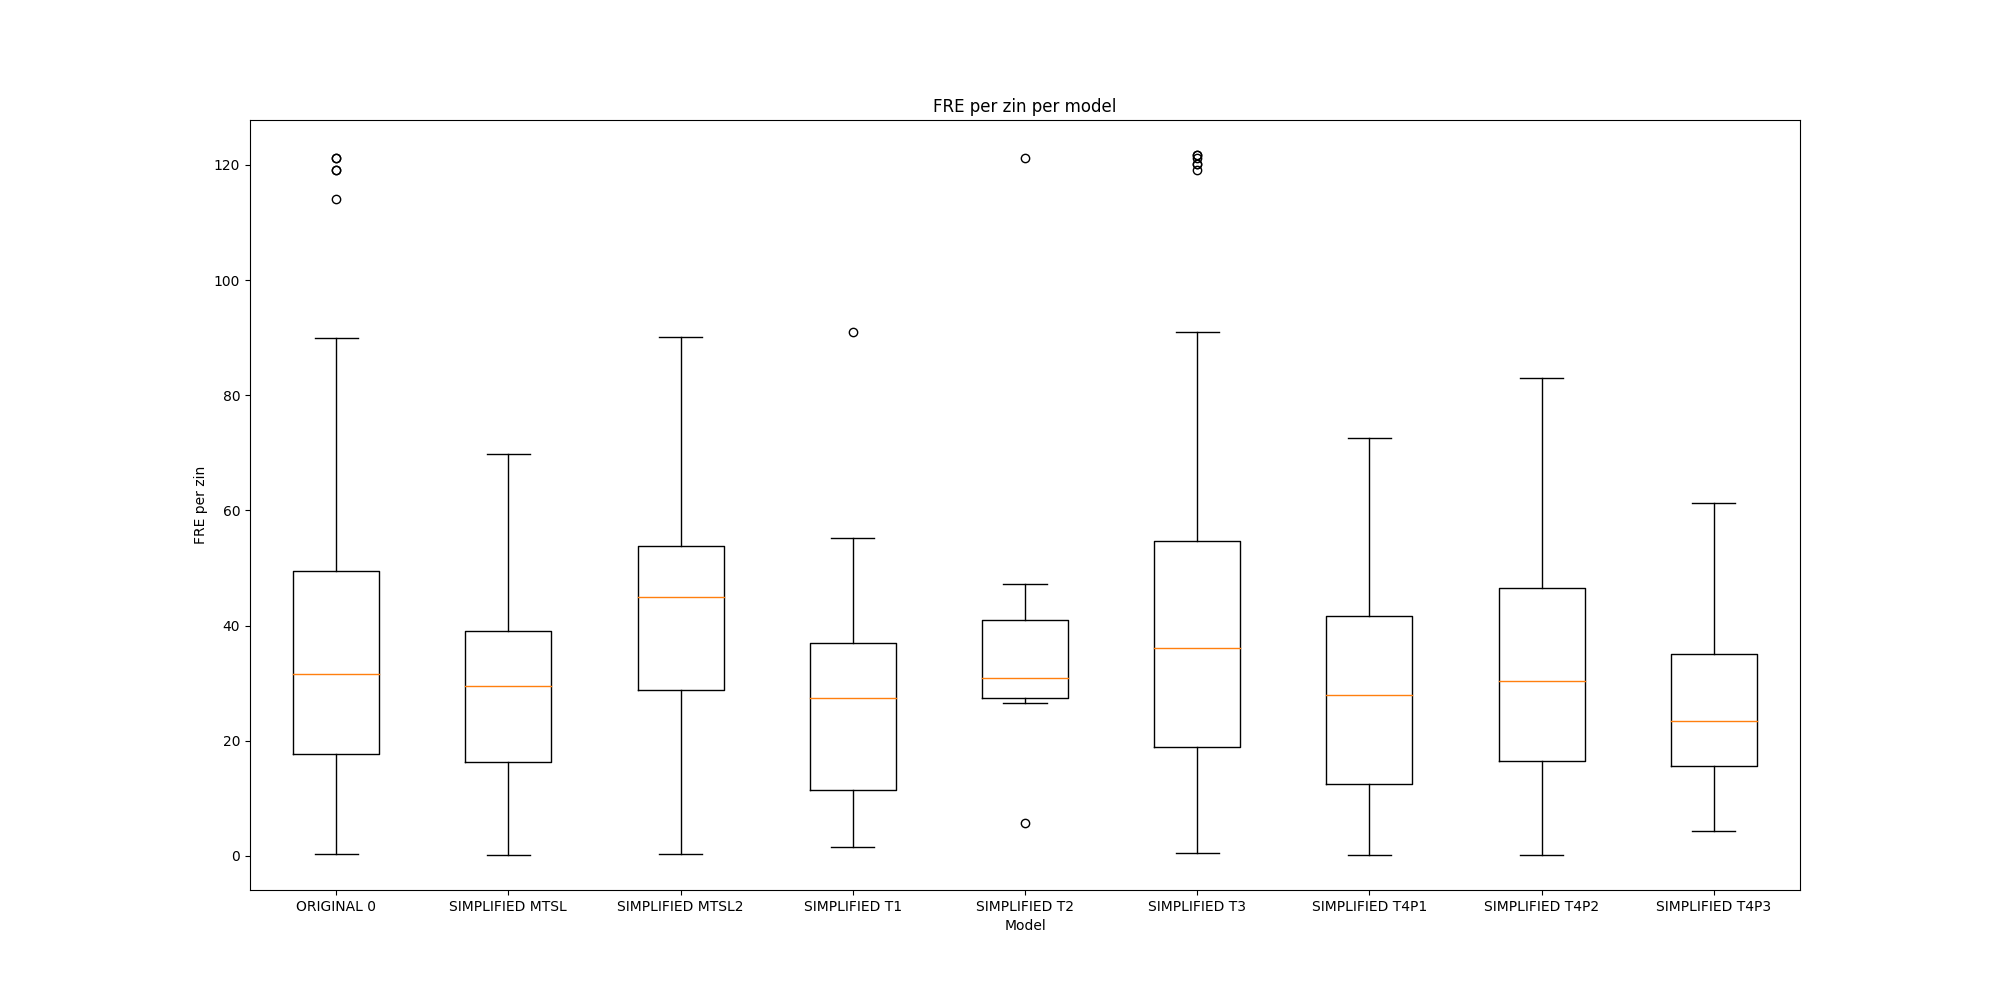
\includegraphics[width=\linewidth]{img/boxplot-fre-a2.png}
	\caption{Boxplot van de FRE-scores voor A2.}
	\label{img:boxplot-fre-a2}
\end{figure}

\begin{figure}
	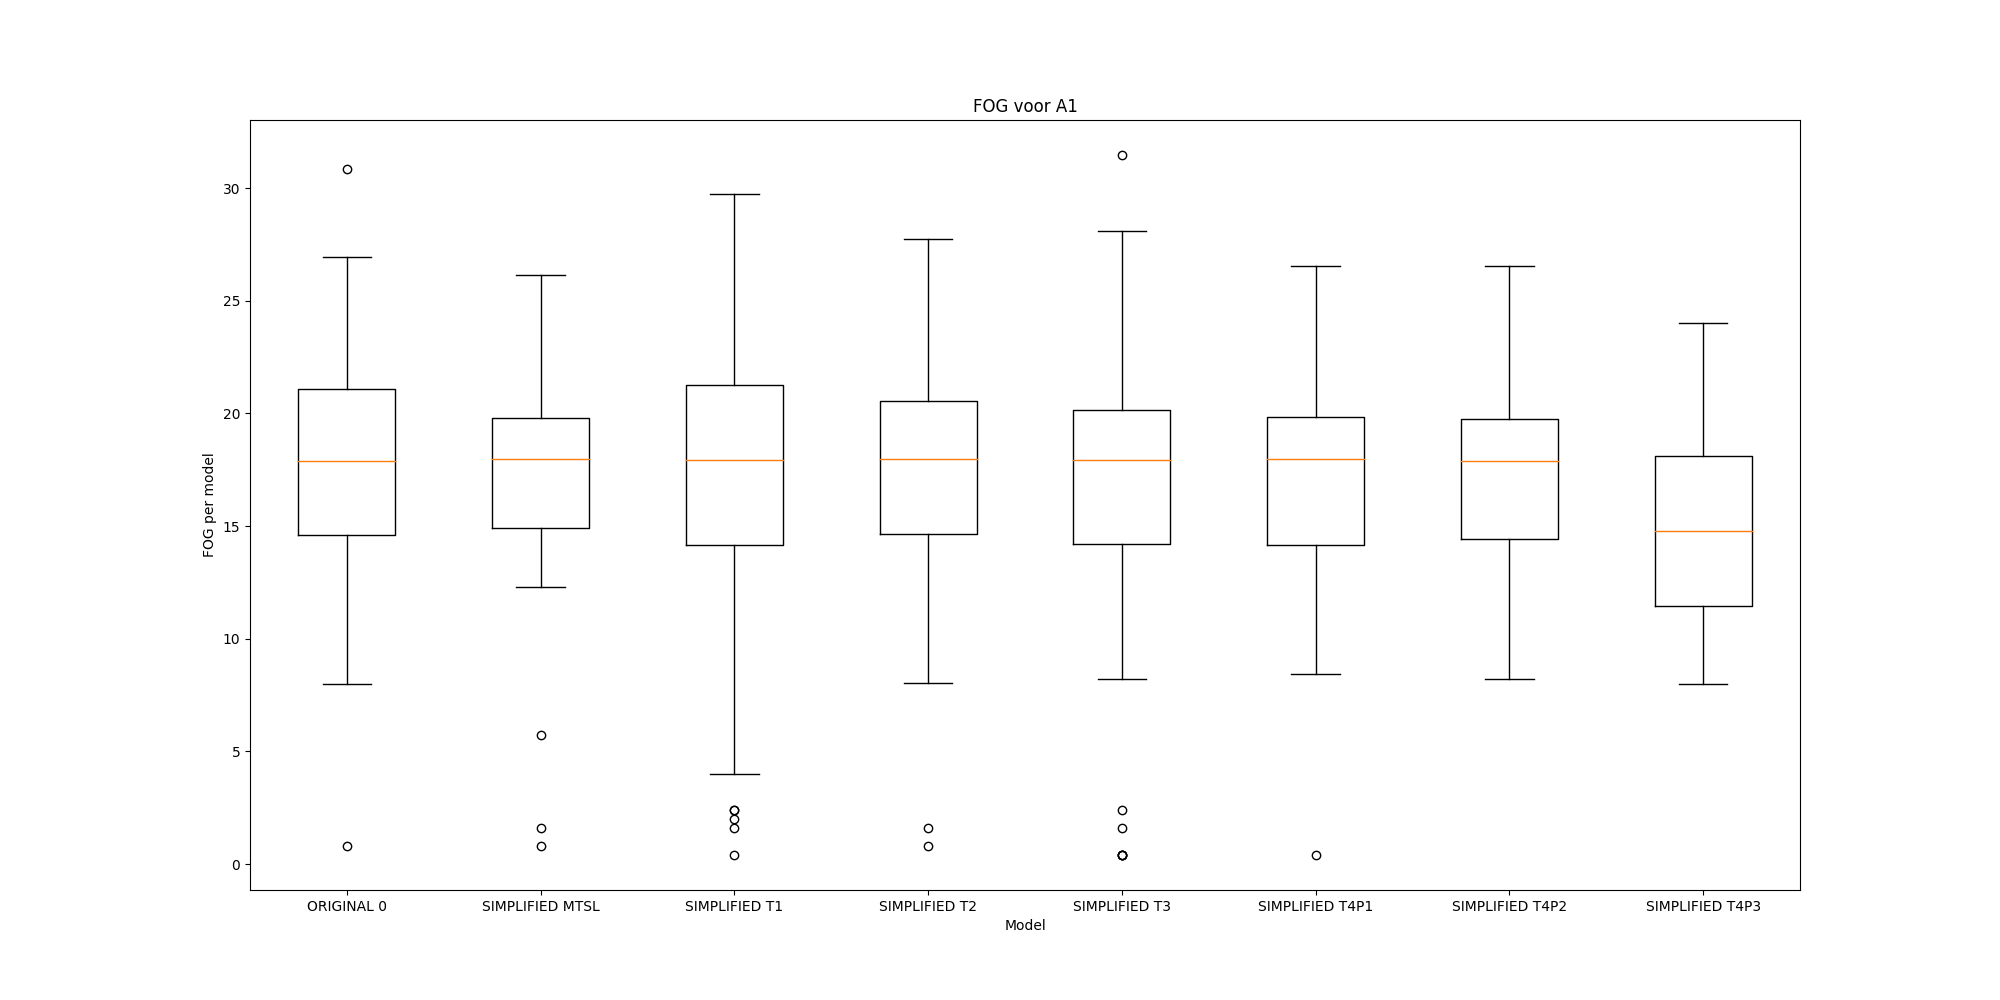
\includegraphics[width=\linewidth]{img/boxplot-fog-a1.png}
	\caption{Boxplot van de FOG-scores voor A1.}
	\label{img:boxplot-fog-a1}
\end{figure}

\begin{figure}
	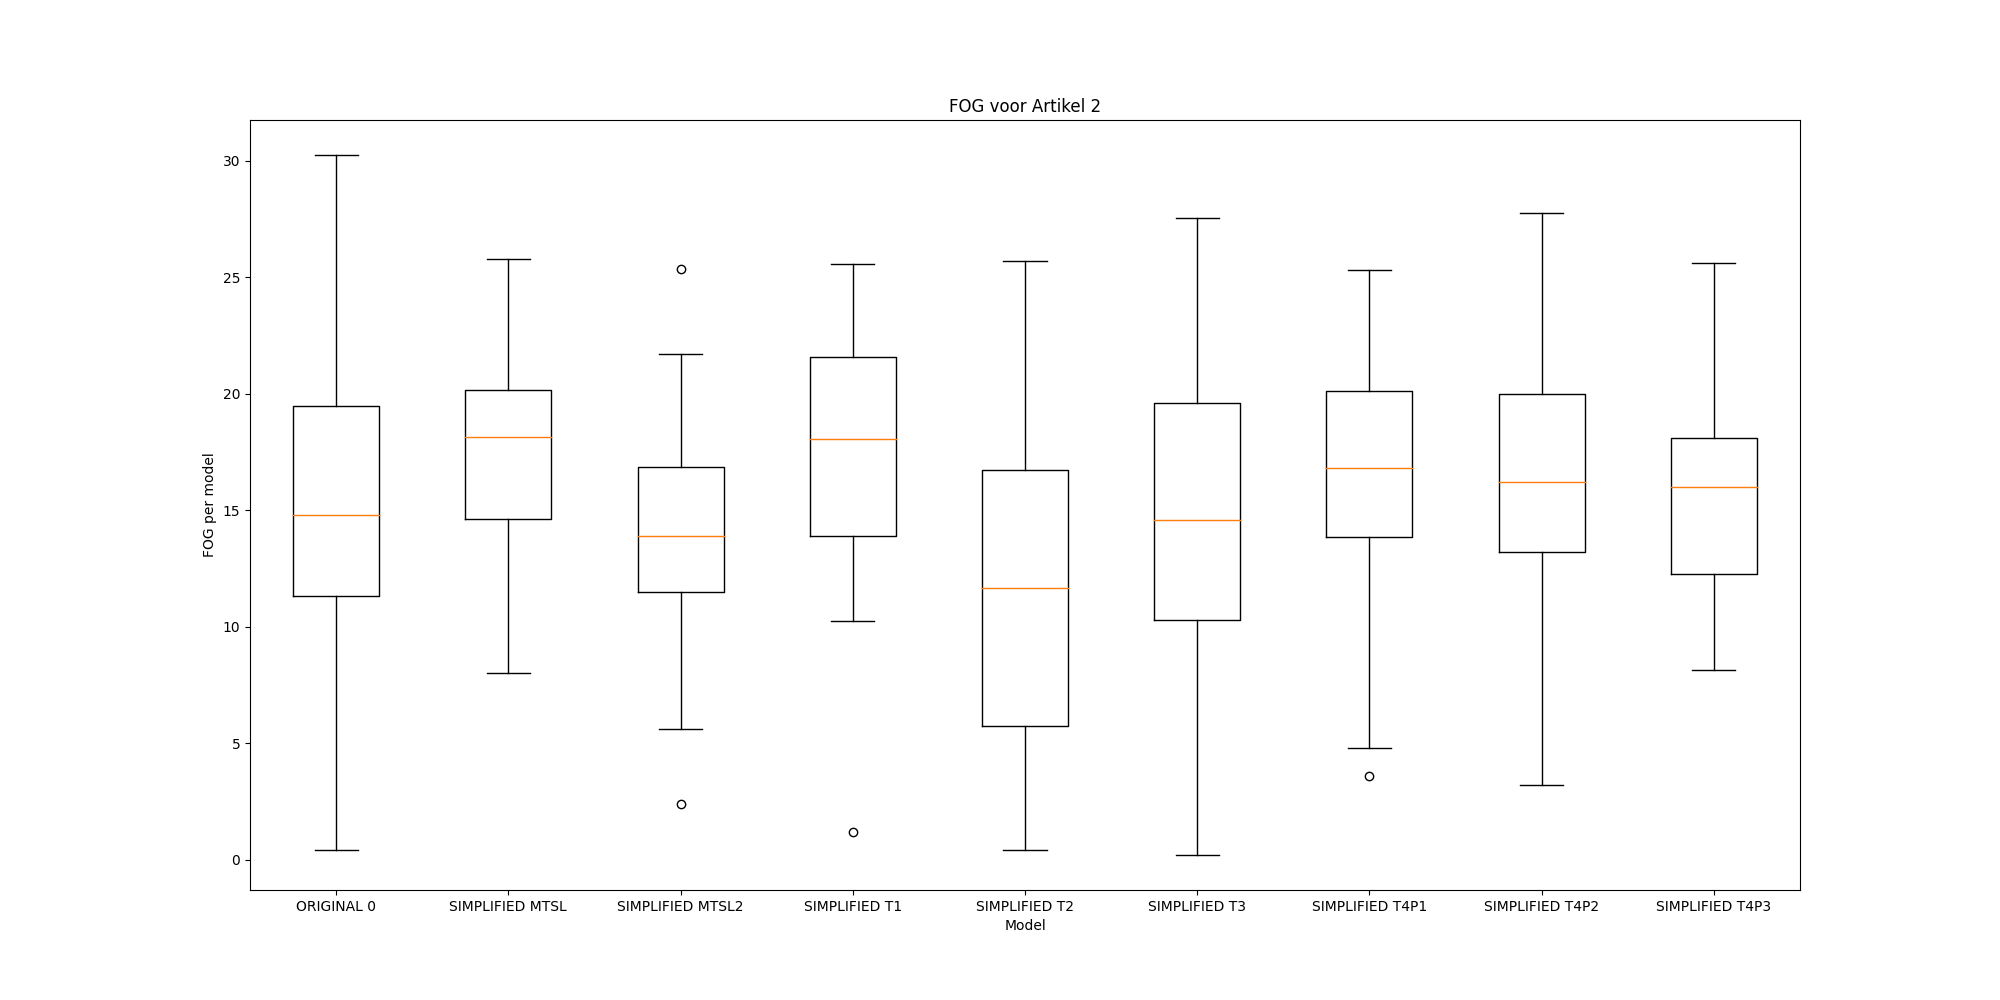
\includegraphics[width=\linewidth]{img/boxplot-fog-a2.png}
	\caption{Boxplot van de FOG-scores voor A2.}
	\label{img:boxplot-fog-a2}
\end{figure}

\begin{figure}
	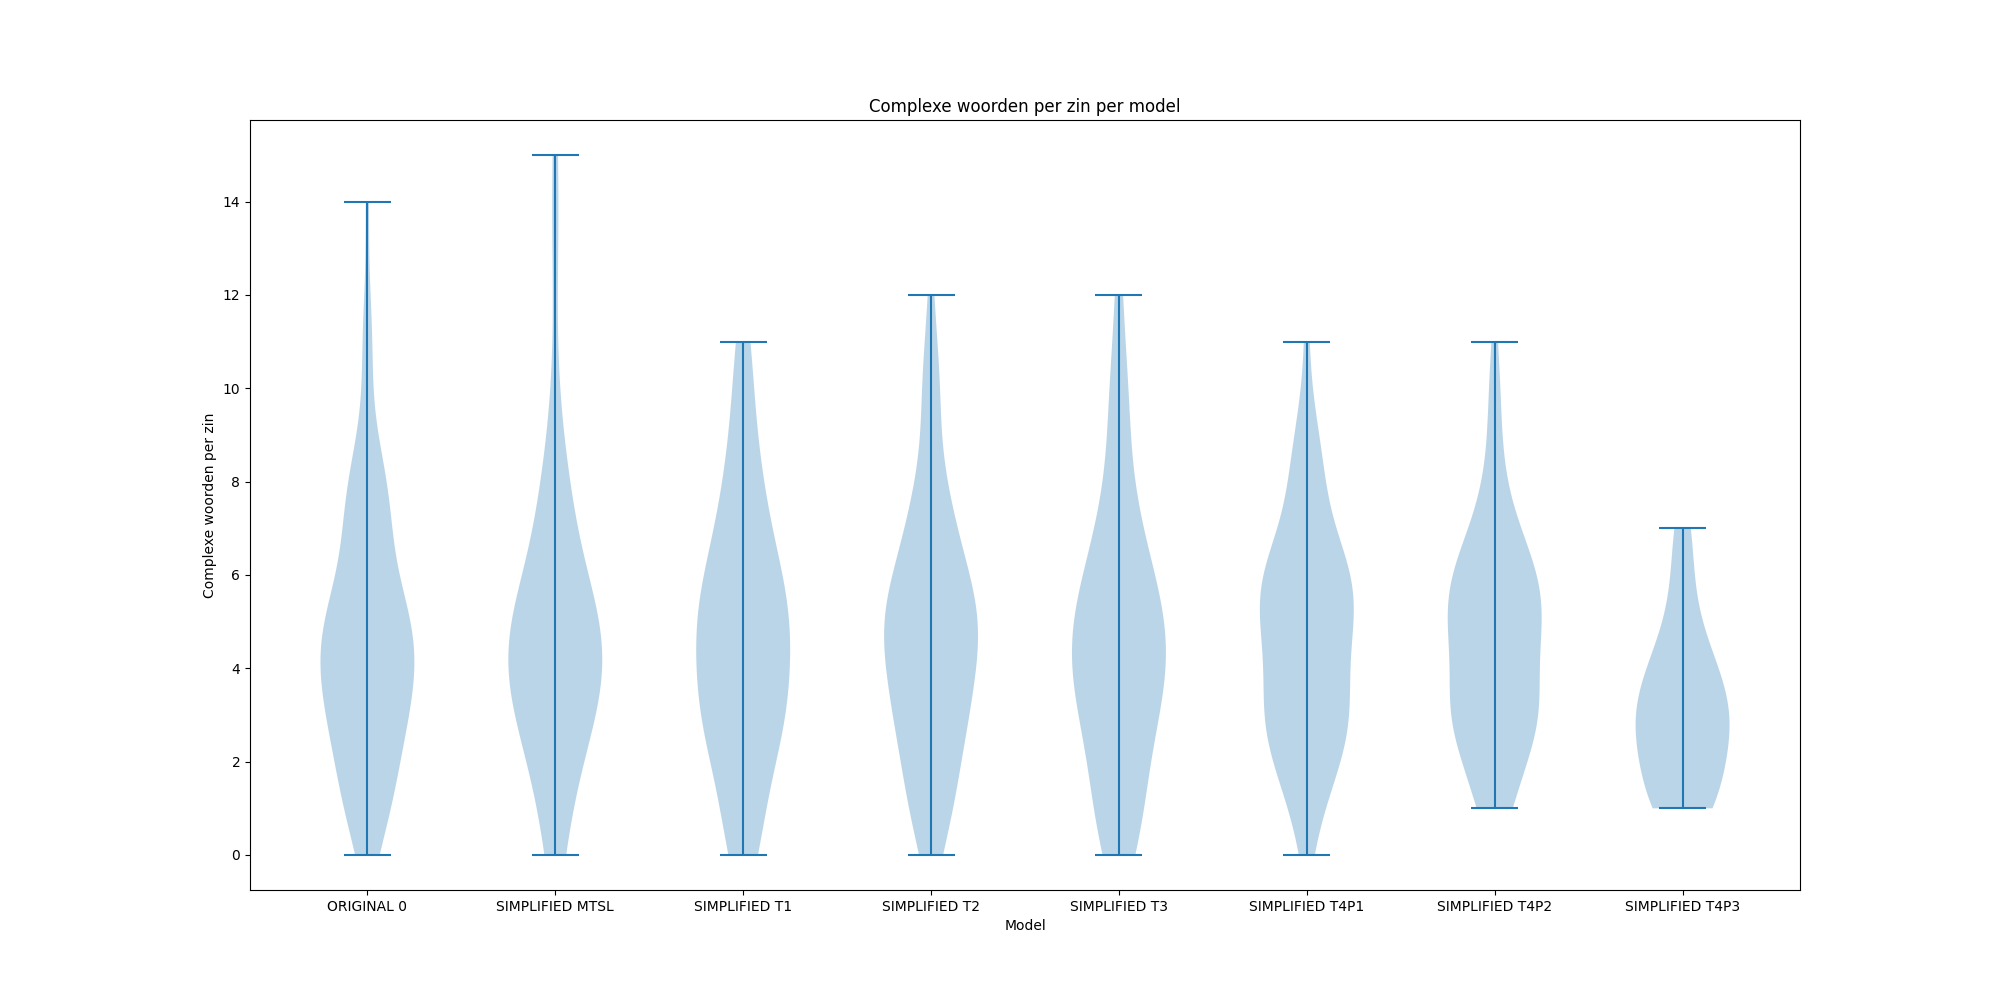
\includegraphics[width=\linewidth]{img/violinplot-complex-a1.png}
	\caption{Gemiddeld aantal complexe woorden per zin gegroepeerd op model voor A1.}
	\label{img:violinplot-complex-a1}
\end{figure}

\begin{figure}
	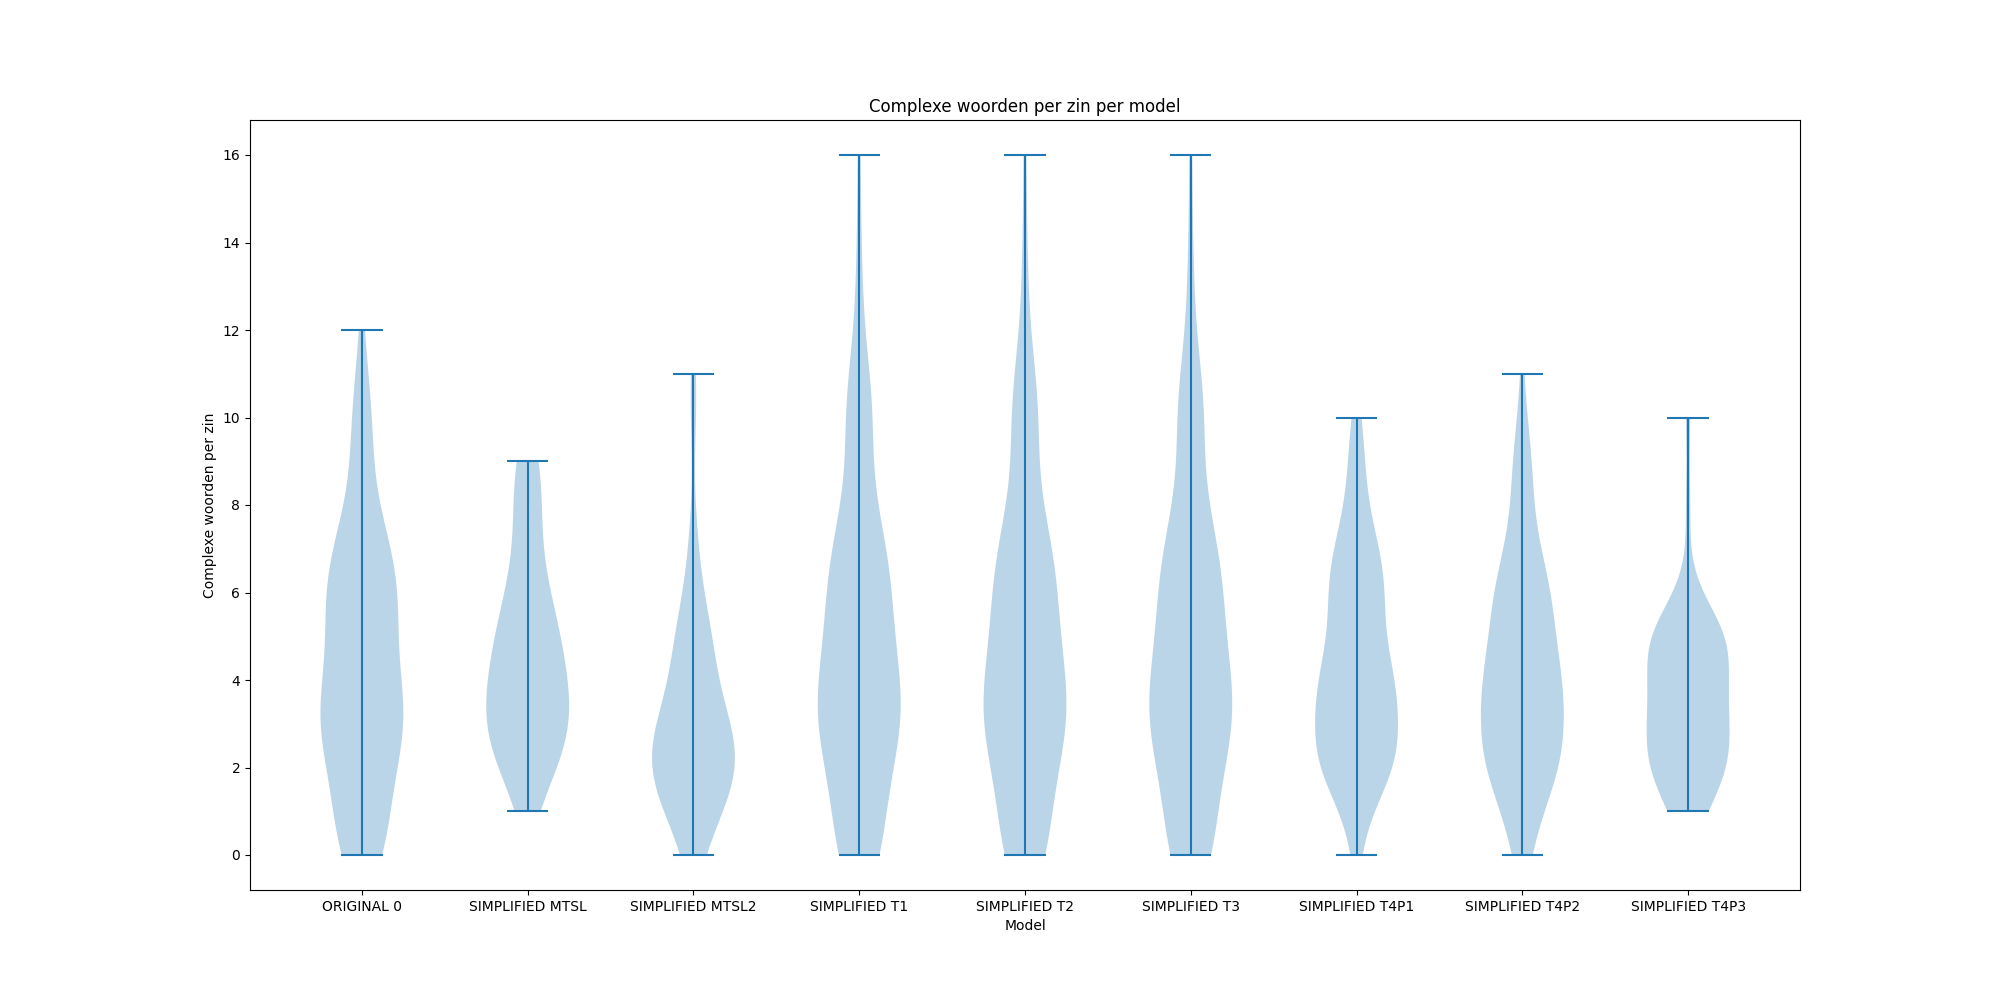
\includegraphics[width=\linewidth]{img/violinplot-complex-a2.png}
	\caption{Gemiddeld aantal complexe woorden per zin gegroepeerd op model voor A2.}
	\label{img:violinplot-complex-a2}
\end{figure}

\begin{figure}
	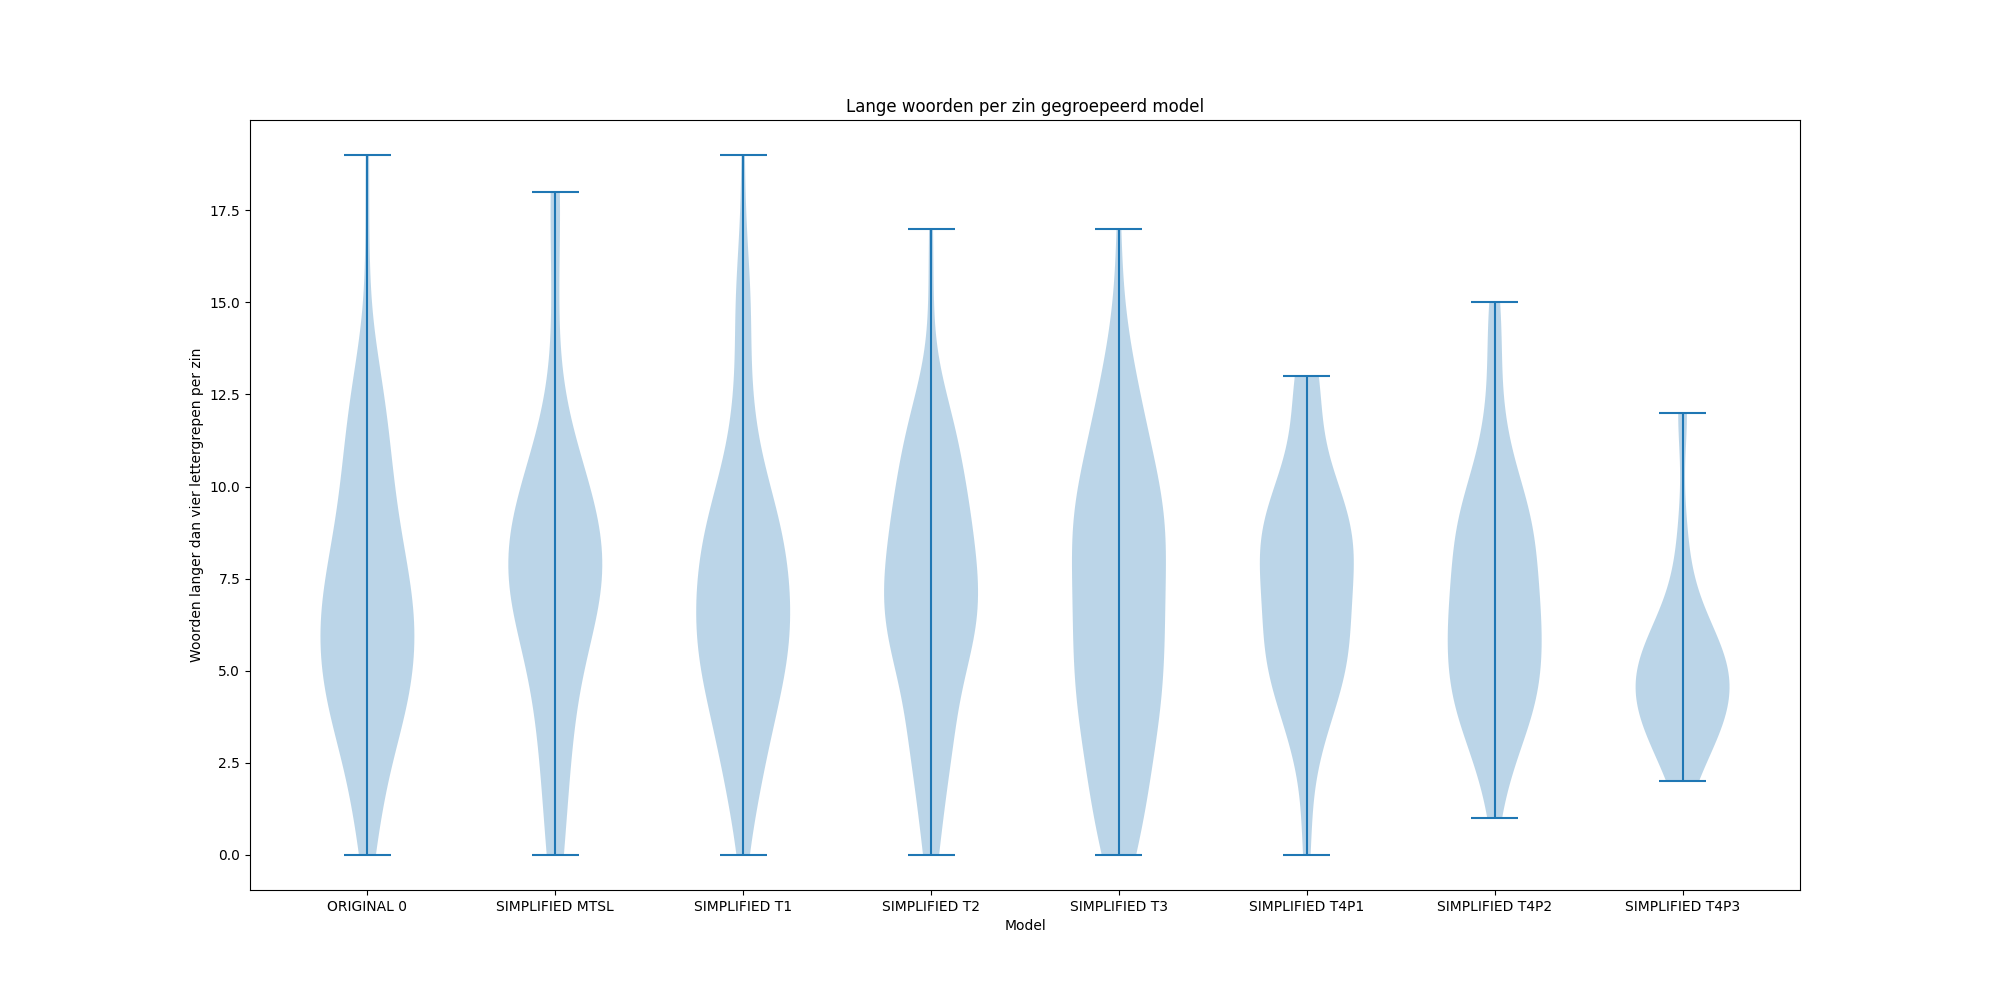
\includegraphics[width=\linewidth]{img/violinplot-long-a1.png}
	\caption{Gemiddeld aantal lange woorden per zin gegroepeerd op model voor A1.}
	\label{img:violinplot-long-a1}
\end{figure}

\begin{figure}
	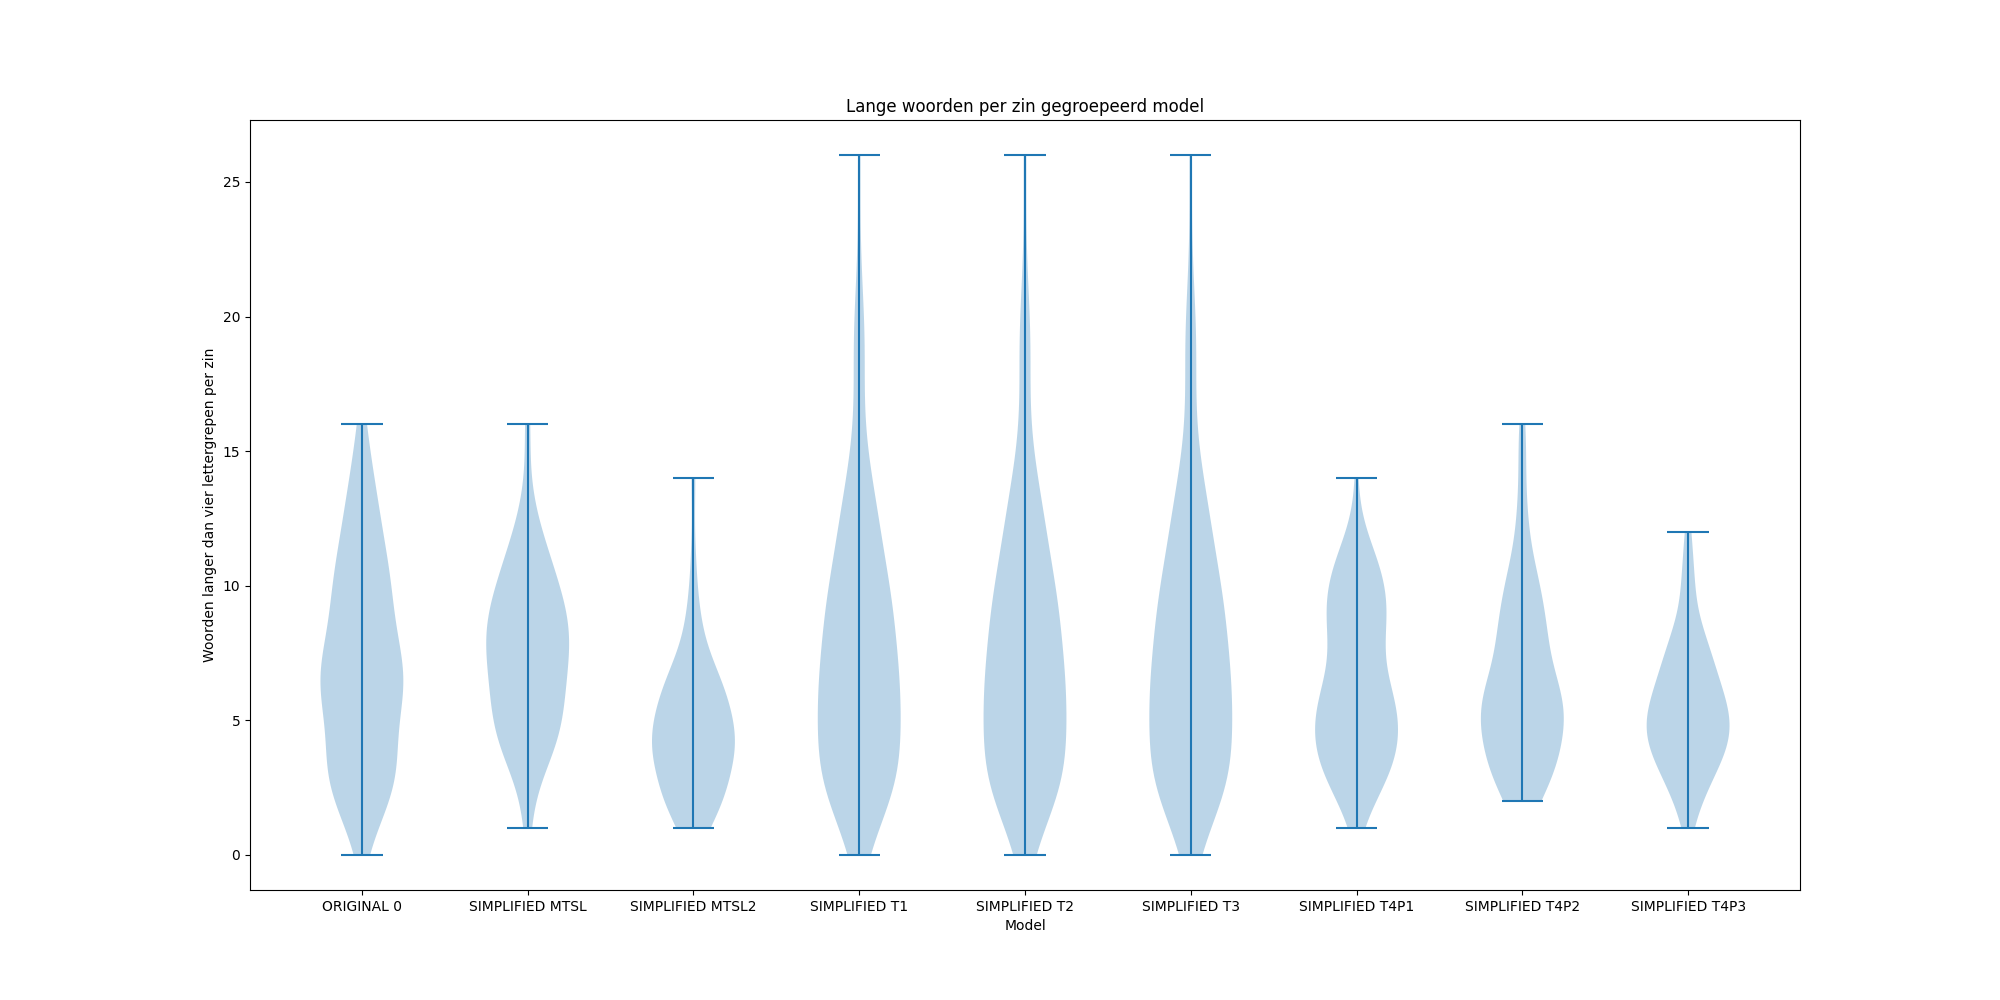
\includegraphics[width=\linewidth]{img/violinplot-long-a2.png}
	\caption{Gemiddeld aantal lange woorden per zin gegroepeerd op model voor A2.}
	\label{img:violinplot-long-a2}
\end{figure}

\begin{figure}
	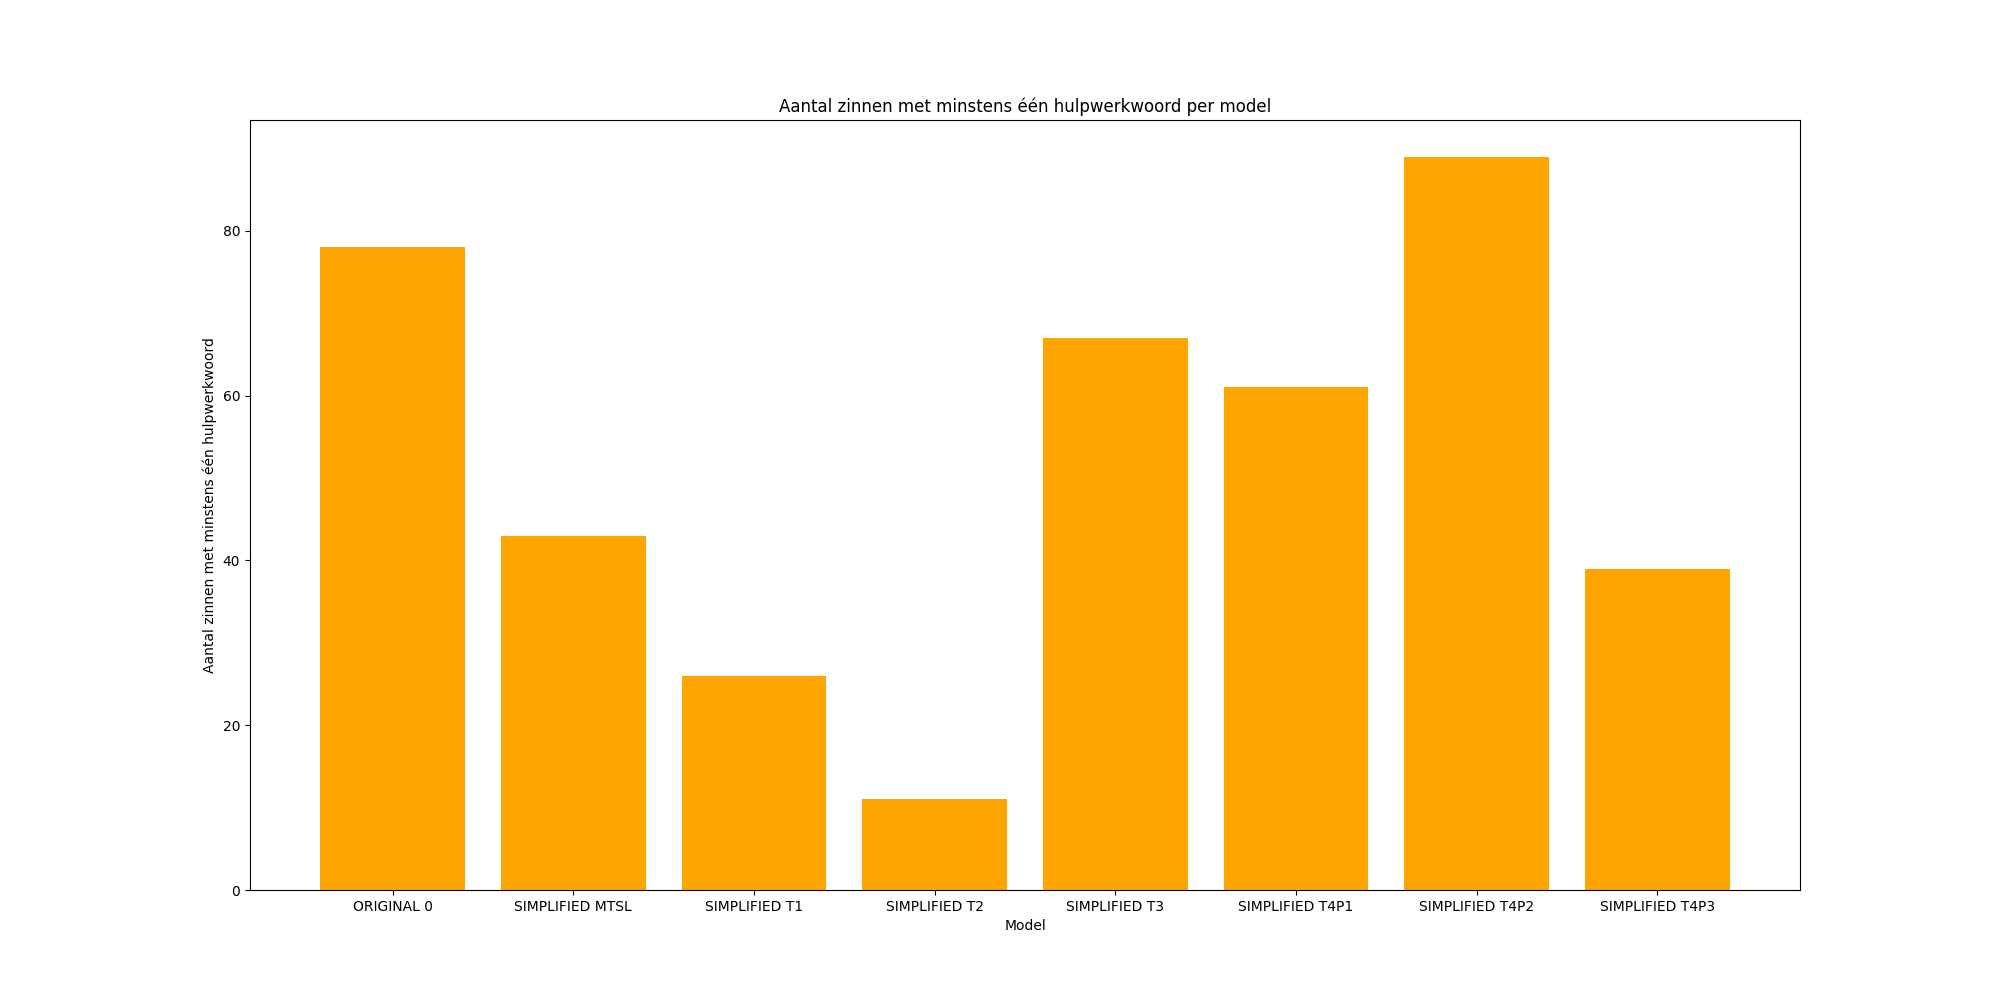
\includegraphics[width=\linewidth]{img/boxplot-aux-a1.png}
	\caption{Gemiddeld aantal hulpwerkwoorden per zin gegroepeerd op model voor A1.}
	\label{img:histplot-aux-a1}
\end{figure}

\begin{figure}
	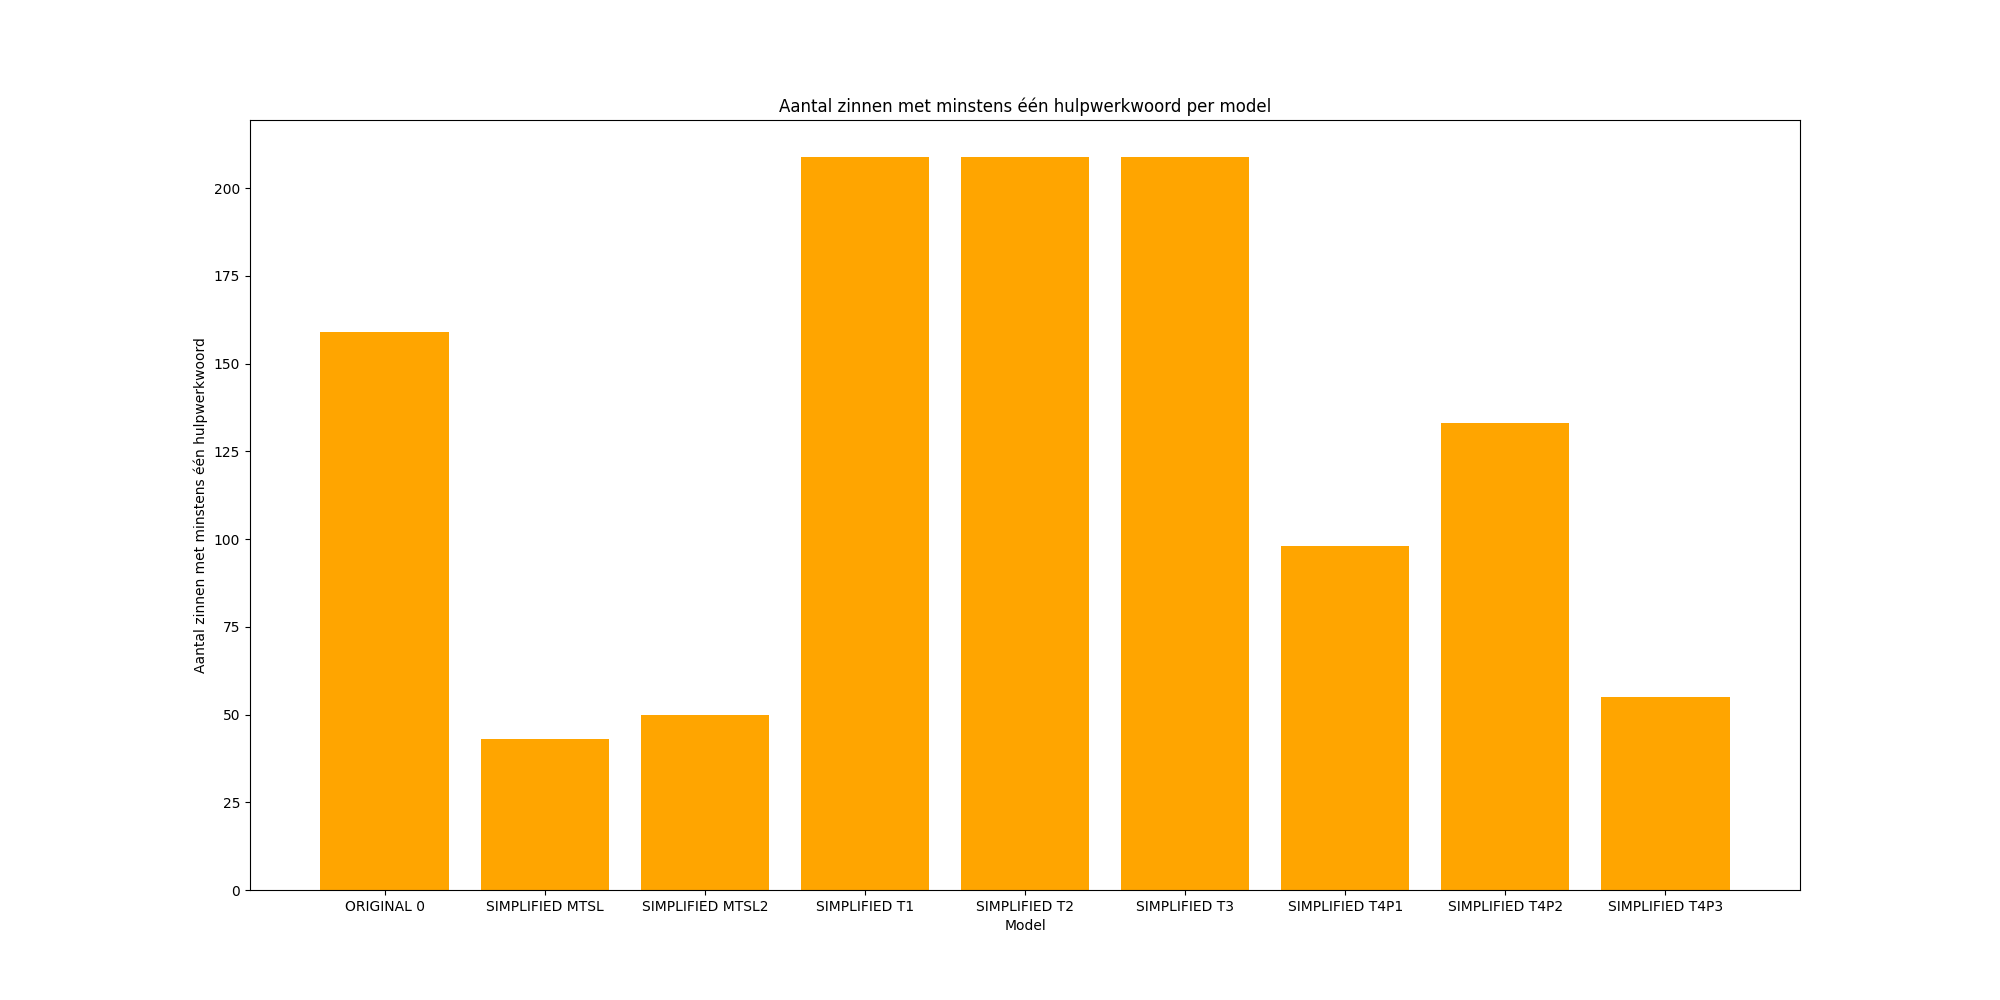
\includegraphics[width=\linewidth]{img/boxplot-aux-a2.png}
	\caption{Gemiddeld aantal hulpwerkwoorden per zin gegroepeerd op model voor A2.}
	\label{img:histplot-aux-a2}
\end{figure}

% tobe

\begin{figure}
	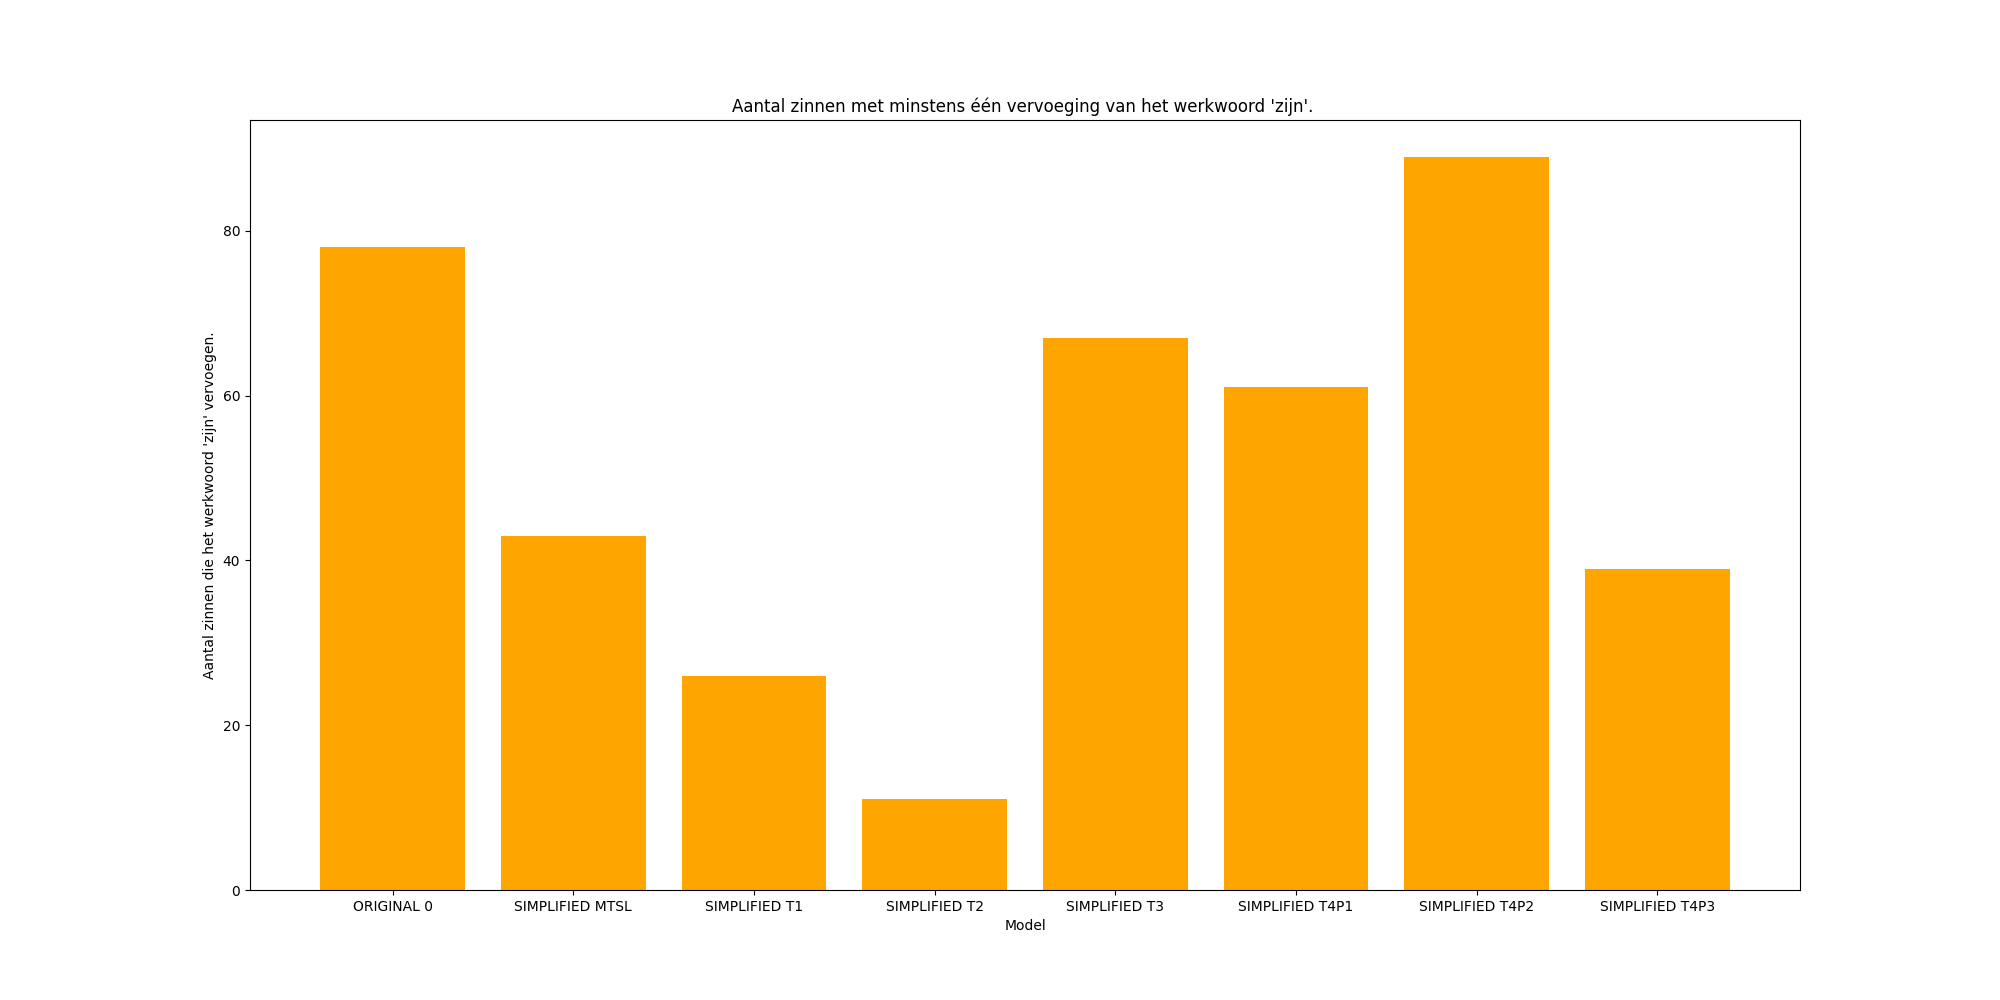
\includegraphics[width=\linewidth]{img/boxplot-tobe-a1.png}
	\caption{Gemiddeld aantal vervoegingen van het werkwoord 'zijn' per zin gegroepeerd op model voor A1.}
	\label{img:histplot-tobe-a1}
\end{figure}

\begin{figure}
	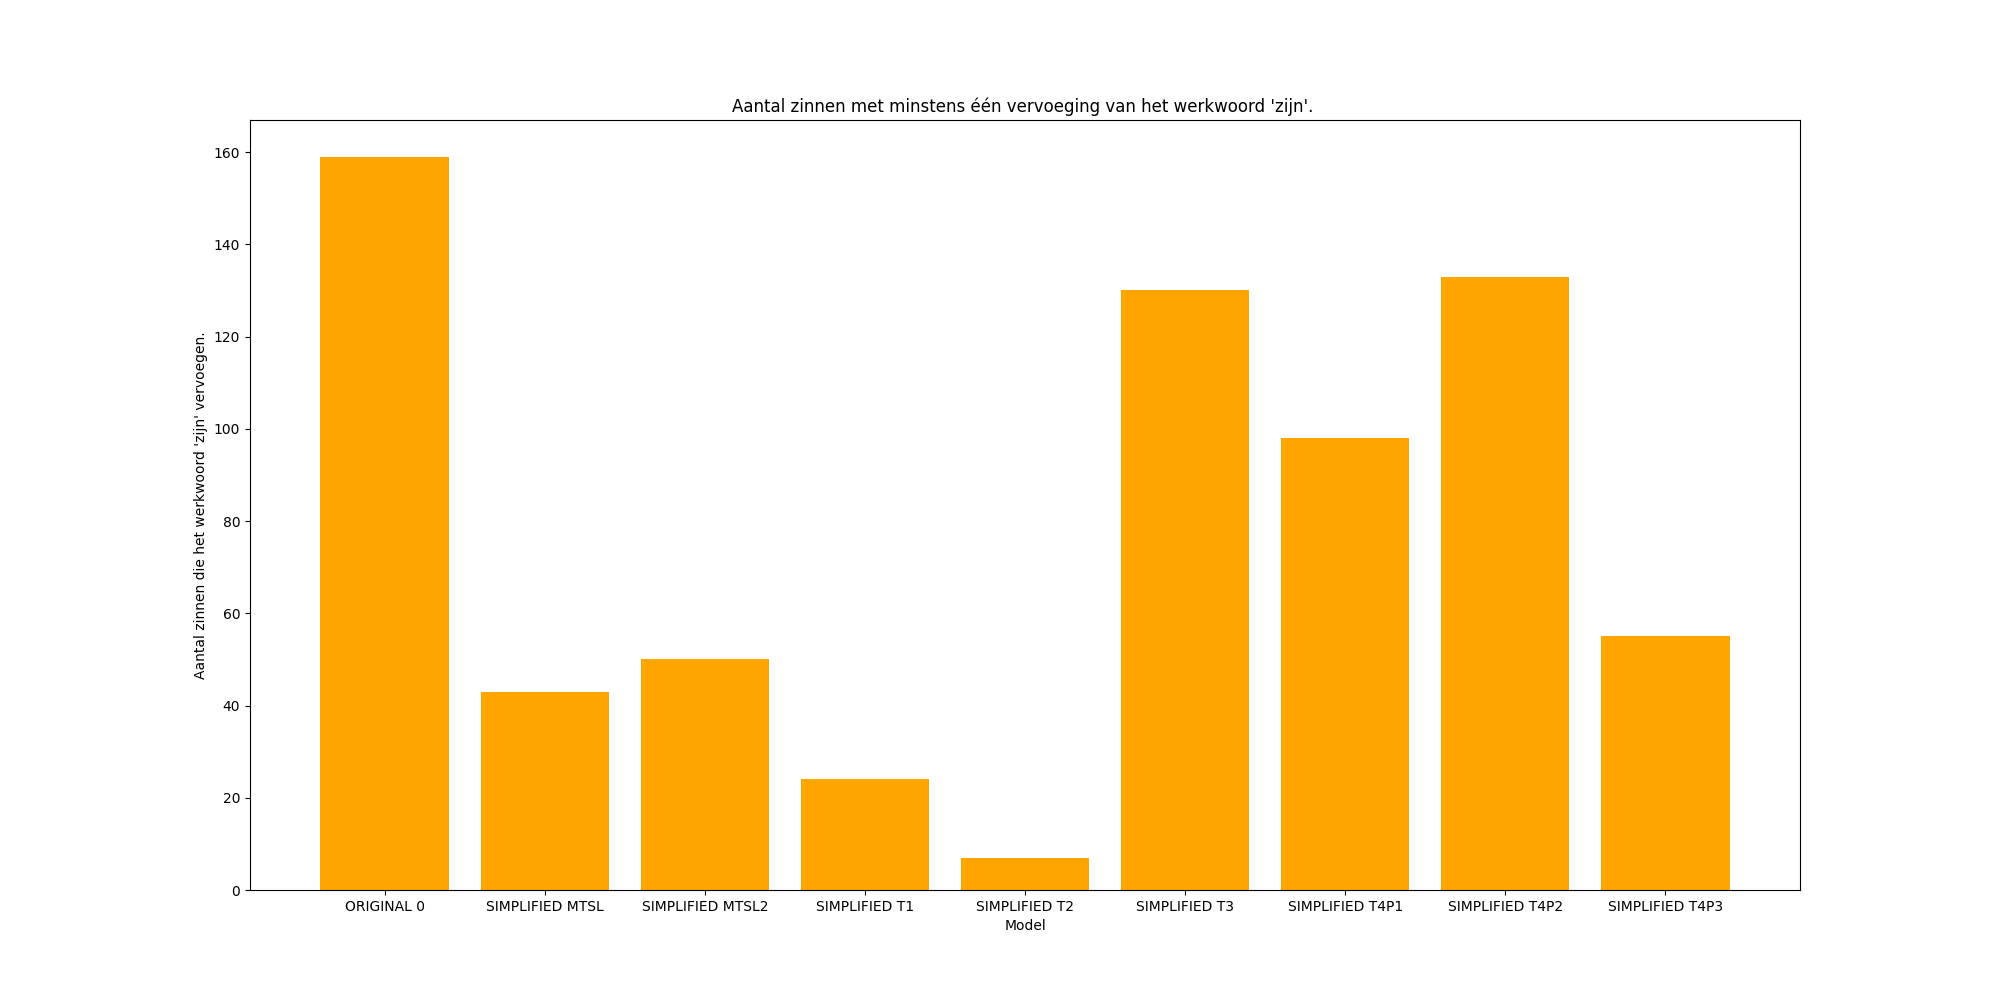
\includegraphics[width=\linewidth]{img/boxplot-tobe-a2.png}
	\caption{Gemiddeld aantal vervoegingen van het werkwoord 'zijn' per zin gegroepeerd op model voor A2.}
	\label{img:histplot-tobe-a2}
\end{figure}
\chapter{\IfLanguageName{dutch}{Schermafbeeldingen van het prototype}{Screenshots prototype}}%
\label{ch:screenshots-prototype}


\begin{center}
	\begin{figure}[H]
		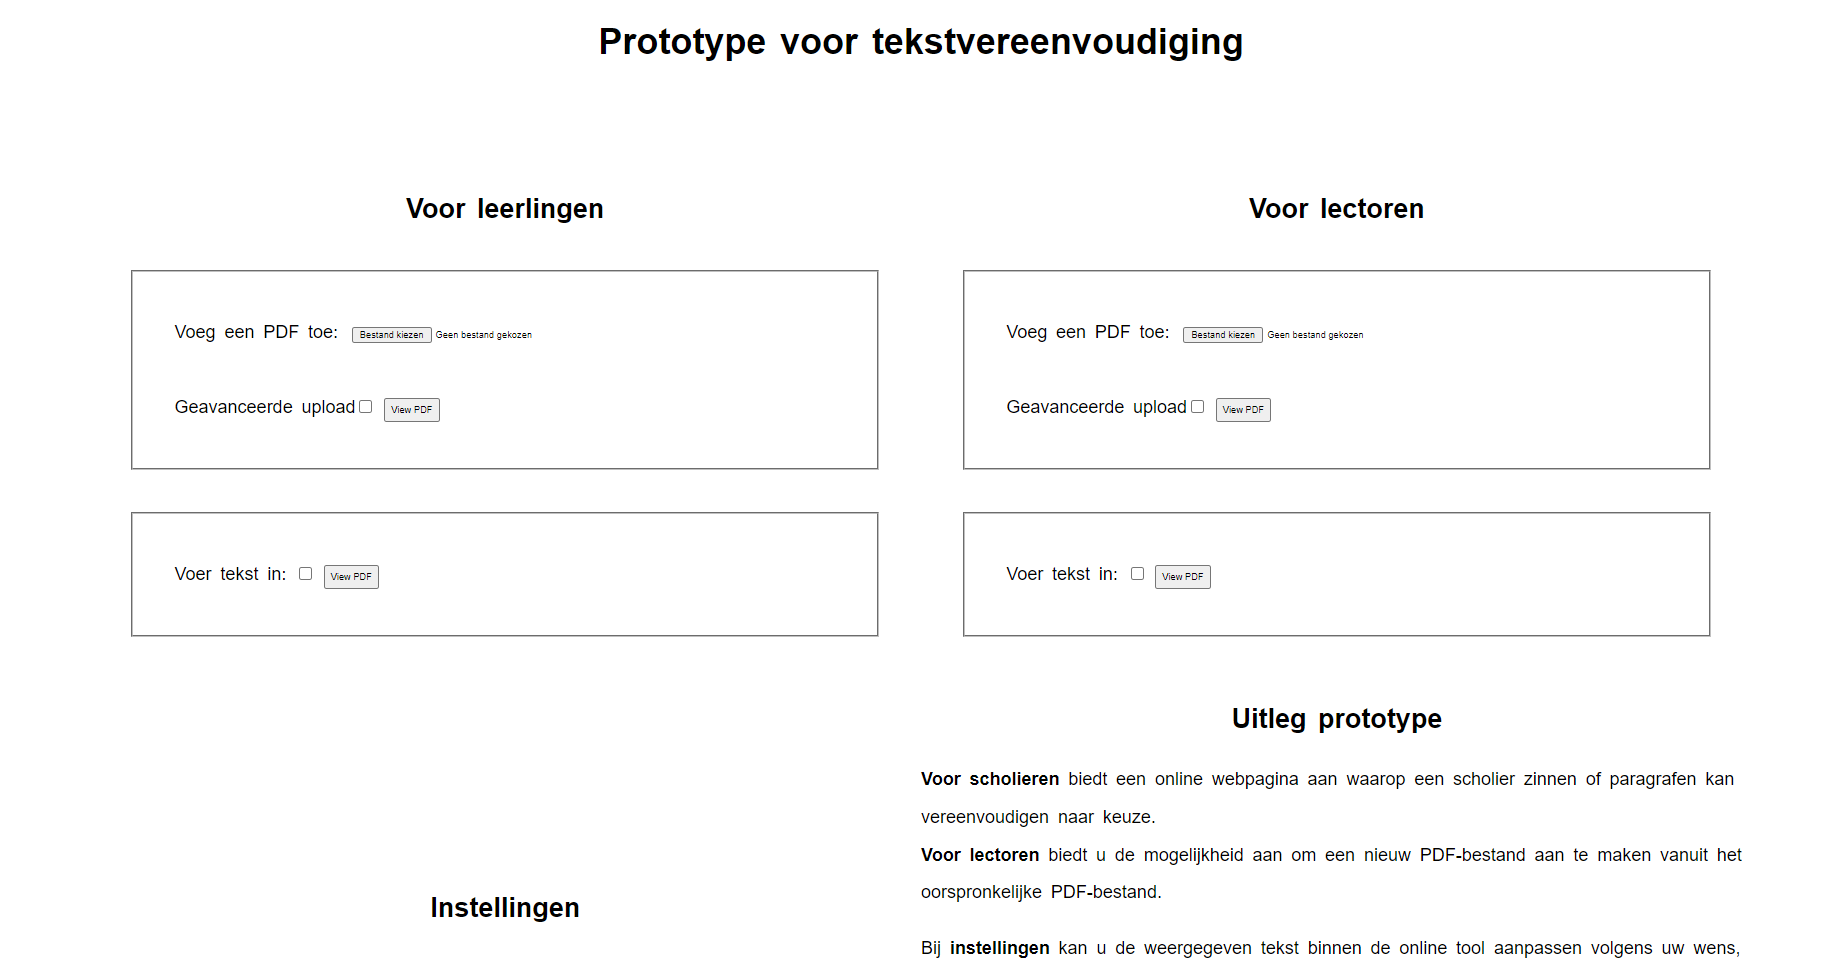
\includegraphics[width=\linewidth]{img/proto-homescreen.png}
		\caption{Een mogelijke weergaven van de homepagina.}		
		\label{img:homepage}
	\end{figure}
\end{center}

\begin{center}
	\begin{figure}[H]
		\includegraphics[width=\linewidth]{img/website-instellingen.png}
		\caption{Voorbeeldweergave van de instellingenpagina.}
		\label{img:website-instellingen}
	\end{figure}
\end{center}

\begin{figure}
	\includegraphics[width=\linewidth]{img/proto-lerarencomponent.png}
	\caption{Een mogelijke weergave van het lerarencomponent met het wetenschappelijk artikel van \textcite{VanBrakel2022} als input.}
	\label{img:proto-lerarencomponent}
\end{figure}

\begin{center}
	\begin{figure}[H]
		\includegraphics[width=\linewidth]{img/proto-melding.png}
		\caption{Een voorbeeldweergave van het scholierencomponent.}
		\label{img:proto-homescreen-scholieren}
	\end{figure}
\end{center}

\begin{center}
	\begin{figure}[H]
		\includegraphics[width=\linewidth]{img/proto-pos-tagging.png}
		\caption{Een voorbeeldweergave van de toepassing van PoS-tagging bij het scholierencomponent.}
		\label{img:proto-pos-tagging-scholieren}
	\end{figure}
\end{center}

\begin{center}
	\begin{figure}[H]
		\includegraphics[width=\linewidth]{img/proto-opsomming-1.png}
		\caption{Stap 1 van een gepersonaliseerde tekstvereenvoudiging in het scholierencomponent.}
		\label{img:proto-scholieren-step-1}
	\end{figure}
\end{center}

\begin{center}
	\begin{figure}[H]
		\includegraphics[width=\linewidth]{img/proto-opsomming-3.png}
		\caption{Stap 3 van een gepersonaliseerde tekstvereenvoudiging in het scholierencomponent.}
		\label{img:proto-scholieren-step-3}
	\end{figure}
\end{center}

\begin{center}
	\begin{figure}
		\includegraphics[width=\linewidth]{img/proto-vraagstelling-1.png}
		\caption{Stap 1 bij het stellen van een specifieke vraag bij gemarkeerde tekst.}
		\label{img:step-1-proto-vraagstelling}
	\end{figure}
\end{center}

\begin{center}
	\begin{figure}
		\includegraphics[width=\linewidth]{img/proto-vraagstelling-2.png}
		\caption{Stap 2 bij het stellen van een specifieke vraag bij gemarkeerde tekst.}
		\label{img:step-2-proto-vraagstelling}
	\end{figure}
\end{center}


%%---------- Backmatter, referentielijst ---------------------------------------

\backmatter{}

\setlength\bibitemsep{2pt} %% Add Some space between the bibliograpy entries
\printbibliography[heading=bibintoc]

\end{document}
